\documentclass[12pt,a4paper]{article}
\usepackage[margin=0.85in,includeheadfoot]{geometry}
\usepackage[T1]{fontenc}
\usepackage{newtxtext,newtxmath}
\usepackage{microtype}
\usepackage{graphicx}
\usepackage{booktabs}
\usepackage{tabularx}
\usepackage{array}
\usepackage{enumitem}
\usepackage{amsmath,amssymb}
\usepackage{cite}
\usepackage{url}
\usepackage[hidelinks]{hyperref}
\usepackage{setspace}
\usepackage{titlesec}
\usepackage{fancyhdr}
\usepackage{tocloft}
\setstretch{1.12}
\setlength{\parindent}{1.2em}
\setlength{\parskip}{4pt}
\setlength{\floatsep}{14pt plus 3pt minus 3pt}
\setlength{\textfloatsep}{16pt plus 3pt minus 3pt}
\setlength{\intextsep}{14pt plus 3pt minus 3pt}
\titleformat{\section}{\Large\bfseries}{\thesection}{0.65em}{}
\titleformat{\subsection}{\large\bfseries}{\thesubsection}{0.65em}{}
\titleformat{\subsubsection}{\normalsize\bfseries}{\thesubsubsection}{0.65em}{}
\titlespacing*{\section}{0pt}{18pt plus 3pt minus 2pt}{8pt}
\titlespacing*{\subsection}{0pt}{12pt plus 2pt minus 2pt}{5pt}
\pagestyle{fancy}\fancyhf{}\fancyhead[L]{\small Road Accident Detection Project Report}\fancyhead[R]{\small Amrita Vishwa Vidyapeetham}\fancyfoot[C]{\thepage}\renewcommand{\headrulewidth}{0.4pt}\setlength{\headheight}{14pt}
\title{AI-Based Road Accident Detection, Severity Assessment, and Emergency Alert System for Nearby Hospitals\\[0.4em]\large Comprehensive Project Report}
\author{Pavan Aditya \quad G Sri Harsha \quad M Pallavi\\[0.35em]
\small Department of Computer Science and Engineering, Amrita Vishwa Vidyapeetham\\
\small M Pallavi: Junior Grade}
\date{October 2026}
\begin{document}
\maketitle
\begin{abstract}
This comprehensive project report documents the design, saved training results, data inventory, video integration, web application, and operational limitations of an AI-based road accident monitoring prototype. Three YOLO26n experiments cover accident interactions, visual severity, and nighttime road-user detection. The accident detector records final validation precision/recall/mAP@0.5/mAP@0.5:0.95 of 94.701/91.308/97.321/84.124\%; the severity model records 76.174/77.897/82.157/60.530\% and separate test values of 79.74\% precision, 71.81\% recall, 80.45\% mAP@0.5, and 55.47\% mAP@0.5:0.95. The nighttime road-user run records 83.960/77.684/85.307/57.371\% on validation. The report analyzes the model plots, data imbalance, temporal video logic, demo summaries, FastAPI dashboard, facility lookup, and alert workflow. Code inspection identifies non-gating context checks, a geographically unsafe facility fallback, and in-memory unauthenticated alerts. Results are repository artifacts, not independently reproduced, and do not establish emergency-service readiness.
\end{abstract}
\clearpage
\tableofcontents
\clearpage
\listoffigures
\clearpage
\listoftables
\clearpage
\pagenumbering{arabic}
\noindent\textbf{Keywords:} 
traffic accident detection, video analytics, YOLO26, severity classification, temporal verification, emergency response, computer vision


\section{Introduction}
Road traffic injuries remain a global public-health concern: the World Health Organization estimates 1.19 million road traffic deaths in 2021 \cite{who2023}. The time between a collision and the arrival of appropriate assistance can be consequential. Surveillance cameras offer broad visual coverage of roads, intersections, and highways. Yet human operators cannot continuously inspect every stream with equal attention, especially when camera networks scale. Automated video analysis can help flag candidate incidents and route them for review, but building a reliable system requires more than a detector with a high frame-level score.

A complete incident workflow contains several distinct technical questions. Does a frame contain objects or visual patterns associated with a crash? Do these detections persist and evolve as a genuine collision event across time? What degree of severity can be inferred from the visible scene? Where did the incident occur, which response facility is appropriate, and was the alert acknowledged? Each stage has separate labels, data requirements, error costs, and performance measures. A strong object-detection score does not itself establish that an accident was confirmed correctly, severity was calibrated, a hospital was selected correctly, or a responder acted faster.


This report expands the project presentation into a comprehensive analysis of the implemented prototype and its available evidence. It documents the intended pipeline and code-level behavior; analyzes model and integration results; reviews accident-video datasets and related work; identifies reproducibility, software, and safety gaps; and proposes a staged improvement and validation plan. Project-specific results are attributed to saved files or source code. The comparison graph is included as supplied, and its values are not presented as a new experiment.

The remainder of this paper presents the problem and related work, system architecture, data and training methods, model results, integration analysis, limitations, recommendations for reproducible evaluation, and conclusions.

\section{Problem Definition and Evaluation Objectives}
\subsection{From frame detection to incident response}
Let a camera stream be a sequence of frames $X=(x_1,x_2,\ldots,x_T)$ at sampling interval $\Delta t$. A frame detector returns candidate boxes and class scores $D_t=\{(b_{tj},c_{tj},p_{tj})\}_{j=1}^{n_t}$, where $b$ is a bounding box, $c$ is a class label, and $p$ is a confidence value. A traffic accident system must then infer whether a sequence forms a real event $E$, estimate severity $S$, associate the event with a location $L$, and produce a response record $R$. The overall pipeline can be represented as
\begin{equation}
X \rightarrow D_{1:T} \rightarrow E \rightarrow S \rightarrow (L,H) \rightarrow R,
\end{equation}
where $H$ denotes a candidate hospital or emergency facility. Each arrow introduces potential errors and delay.

Frame-level accident recognition, temporal event localization, and accident anticipation are related but non-identical tasks. Recognition asks whether evidence of an accident is visible now. Temporal localization estimates when an event begins and ends in a clip. Anticipation predicts a collision before it occurs. This project reports temporal verification after initial detections; the report does not claim a prediction-before-impact capability. That distinction matters when interpreting its intended public-safety benefit.

Severity estimation is likewise a different target from accident detection. A detector may identify a collision class while a severity model estimates low, moderate, or high consequence from visual cues. Visible damage, object size, occlusion, camera angle, and post-impact motion may not reveal injury status. A vision model should therefore be described as estimating visual incident severity, not diagnosing injuries or replacing emergency triage.

\subsection{System-level objective}
The project goal is an assisted monitoring workflow rather than an autonomous dispatch authority. A practical objective is to maximize correct and timely incident awareness while controlling false alarms, missed events, and unsafe severity overstatement. A general cost function can be written as
\begin{equation}
J = \lambda_{FN} FN + \lambda_{FP} FP + \lambda_{D}D + \lambda_{S}E_S + \lambda_{A}E_A,
\end{equation}
where $FN$ and $FP$ are missed and false incidents, $D$ is detection-to-alert delay, $E_S$ is severity estimation error, $E_A$ is alert-routing or acknowledgement error, and $\lambda$ terms express operational costs. The project report supplies detector metrics but does not quantify this end-to-end objective.

For a safety-support system, sensitivity to genuine events, precision under rare-event prevalence, delay distributions, and alert reliability all matter. A high average precision does not specify the operating threshold or false-alert burden per camera-hour. Nor does it measure a downstream operator's ability to act. An evaluation must consequently report both component metrics and operational workflow measures.

\section{Related Work}
\subsection{Accident detection, anticipation, and temporal evidence}
Fang et al. survey vision-based traffic accident detection and anticipation and emphasize the long-tailed, dynamic, uncertain, and distribution-shifted nature of accident data \cite{fang2024}. Their task taxonomy provides a useful caution: frame classification, temporal detection, and risk anticipation should not be collapsed into one accuracy figure. Recent crash and near-crash recognition using dashcam streams operates under moving-camera conditions that differ from fixed roadside CCTV \cite{shi2024two}. More surveillance-oriented benchmarks explicitly target freeway camera views and real incidents \cite{xu2022tad,zimmer2025}.

Temporal evidence can reduce errors caused by a single transient frame prediction, but it can also add latency and introduce failure modes. A threshold requiring consecutive positive frames may suppress isolated false detections, while missing short or partially occluded collisions. Optical flow, recurrent units, temporal transformers, tracking, or rule-based event state machines are alternative mechanisms. Fine-grained accident detection research explicitly combines temporal-spatial localization, collision classification, and severity estimation, while two-stream work fuses temporal and spatial signals for crash and near-crash identification \cite{yu2024fine,shi2024two}. The project report states that a temporal verification stage is present, but does not specify its window length, threshold, state transitions, track association method, or measured effect. We therefore treat verification as an architectural function, not as a quantified improvement.

Accident benchmarks have begun to address rare, safety-critical events from multiple viewpoints. The TUM Traffic Accid3nD dataset contributes real highway accident data with varied sensor annotations and explicitly discusses the scarcity and domain specificity of accident data \cite{zimmer2025}. The ACCIDENT benchmark introduced in 2026 includes real and synthetic CCTV clips with temporal and spatial localization and collision-type tasks, alongside in-distribution and out-of-distribution evaluation \cite{picek2026}. These resources highlight that a small image collection and a clip-level CCTV workflow are not interchangeable evaluation settings.

\subsection{Object detection as a system component}
Single-stage object detectors are widely used where inference speed and spatial localization are required. YOLO-family models predict object classes and bounding boxes in a shared network, following the one-stage detection formulation introduced by Redmon et al. and later versions \cite{redmon2016,redmon2018}. The YOLO26 family is described by its authors as a unified real-time detector with a native end-to-end path and task variants \cite{jocher2026}. The project identifies YOLO26n, the nano scale, as its detector. This selection is plausible for constrained inference, but a claim of real-time operation still requires measured throughput, hardware, image pipeline, batch size, and end-to-end latency under the target camera load.

Precision, recall, and average precision summarize different properties of a detector. Precision measures the fraction of positive predictions that are correct at a selected operating point; recall measures the fraction of ground-truth positives found. Average precision summarizes the precision-recall curve, and mAP averages AP across classes. In the Ultralytics validation convention, mAP@0.5 uses intersection-over-union threshold 0.5, while mAP@0.5:0.95 averages across thresholds from 0.50 to 0.95 in increments of 0.05 \cite{ultralyticsval}. Results depend on class definitions, split composition, label quality, confidence handling, and evaluation implementation. The two reported mAP values are therefore useful but insufficient for deployment readiness.

\subsection{Severity models and response coordination}
Severity classification has been studied using both structured crash records and visual features. Record-based severity prediction uses contextual variables such as road type, vehicles, weather, and crash circumstances; visual severity inference must instead work from incomplete imagery. These targets differ in label provenance and what can be observed by a camera. The project presentation does not identify the severity model architecture or label-generation rubric. The repository adds a three-class YOLO26n run, class counts, a confusion matrix, and test metrics, but does not establish whether the visual classes correspond to injury outcomes. These limits constrain interpretation of class-wise errors and operational meaning.

Emergency notification systems add location services, facility lookup, communication, and workflow status to visual analysis. The capstone describes nearby hospital information, authority and hospital dashboards, alert acknowledgement, and response status. These features address an important systems gap, but the presentation does not provide a live-service test, geocoding accuracy, hospital directory provenance, dispatch integration, delivery/acknowledgement reliability, or response time. We distinguish an implemented prototype flow from a validated emergency communications service.

\subsection{Positioning}
The proposed system's distinguishing aim is integration: candidate crash detection, temporal verification, severity, location, nearby facilities, and dashboards appear in one workflow. Prior research has proposed deep spatiotemporal detection systems and datasets, including an RGB-plus-optical-flow ensemble for accident detection, but the source chart does not provide enough matched protocol detail for a quantitative comparison \cite{ade2024}. Integration is valuable only if its interfaces preserve uncertainty and errors are measured at each stage. This paper consequently evaluates the project as an integrated prototype and does not infer that integration alone improves road-safety outcomes.

\section{System Architecture}
\subsection{Processing stages}
The presentation describes a CCTV/IP-camera input, frame preparation, YOLO26n inference, temporal verification, a severity assessment stage, location/facility association, backend processing, and monitoring dashboards. The functional flow comprises video input, frame preparation, candidate detection, temporal verification, severity estimation, facility lookup, and dashboard alerting.



























\section{Dataset and Experimental Method}
The accident dataset is reported as 7,630 images divided into 5,849 training, 712 validation, and 1,069 test images, with ten labels: bike, car, person, and seven collision-interaction categories. A separate severity dataset contains 4,452 images, split 3,559/447/446, with moderate-accident, no-accident, and severe-accident labels. The repositories also include dataset configuration files and saved evaluation outputs. Counts establish the number of available files, not annotation correctness, event-level independence, or absence of duplicates.

The accident label-distribution plot contains 28,223 boxes. Car boxes contribute 17,577 (62.28\%), compared with 3,606 bikes and 3,514 people. Among the interaction labels, car--car contributes 2,497, while car--person contributes 28 and bike--object only four. Table~\ref{tab:classes} lists all reported counts and AP values visible in the saved precision-recall plot. The bike--object category is absent from that plot, so its class-specific performance cannot be supported. Such skew means aggregate metrics may be dominated by common classes.

\begin{table}[t]\centering\small
\caption{Accident-run box counts and AP@0.5 values shown in the saved plot.}
\label{tab:classes}
\begin{tabular}{lrr}\toprule
Class & Boxes & AP@0.5\\\midrule
Bike & 3,606 & 0.971\\
Bike--bike & 207 & 0.969\\
Bike--object & 4 & --\\
Bike--person & 147 & 0.995\\
Car & 17,577 & 0.989\\
Car--bike & 354 & 0.940\\
Car--car & 2,497 & 0.985\\
Car--object & 289 & 0.968\\
Car--person & 28 & 0.995\\
Person & 3,514 & 0.947\\\bottomrule
\end{tabular}
\end{table}

Saved training arguments identify pretrained YOLO26n, 100 epochs, 640-pixel images, batch size eight, AdamW, seed zero, deterministic mode, patience 20, and validation after training. Augmentations include Mosaic, horizontal flipping, scaling, and HSV perturbation; Mosaic is disabled for the last ten epochs. The baseline run took approximately 13,139 seconds. Severity training took about 7,458 seconds. Hardware and software details are incomplete, and saved dataset paths refer to an earlier absolute root, so exact replay requires confirming the data version and path mapping.

The saved validation protocol reports precision, recall, mAP@0.5, and mAP@0.5:0.95. Precision is $TP/(TP+FP)$ and recall is $TP/(TP+FN)$ at an operating threshold. AP integrates precision over recall; mAP averages class AP. The stricter mAP averages IoU thresholds from 0.50 through 0.95. These are detection metrics; they do not directly measure incident-level sensitivity, false alarms per camera-hour, or severity calibration.

\section{Results}
Table~\ref{tab:metrics} summarizes final-epoch validation results from the saved run CSV files. They are repository records, not independently reproduced measurements. The target labels differ between the two models, so the table is an inventory rather than a ranking.

\begin{table}[t]\centering\small
\caption{Final-epoch validation metrics (\%).}
\label{tab:metrics}
\begin{tabular}{lrrrr}\toprule
Task & Precision & Recall & mAP@0.5 & mAP@0.5:0.95\\\midrule
Accident detection, 10 classes & 94.701 & 91.308 & 97.321 & 84.124\\
Severity, 3 classes & 76.174 & 77.897 & 82.157 & 60.530\\
Night traffic, 5 classes & 83.960 & 77.684 & 85.307 & 57.371\\\bottomrule
\end{tabular}
\end{table}

The accident run's final values are 0.94701 precision, 0.91308 recall, 0.97321 mAP@0.5, and 0.84124 mAP@0.5:0.95. Across epochs, precision peaks at 0.95137 (epoch 99), recall at 0.94558 (epoch 81), mAP@0.5 at 0.97347 (epoch 97), and mAP@0.5:0.95 at 0.84124 (epoch 100). These maxima occur at different epochs and must not be combined as if they came from one checkpoint. The F1 confidence plot peaks near 0.93 at confidence 0.528. This is a candidate validation threshold only; its false-alarm rate on continuous roadside video is unknown.

The training history shows decreasing box, classification, and L1 losses. Final train/validation losses are 0.72378/0.68220 for box, 0.31919/0.29605 for classification, and 0.00469/0.00519 for L1. The lack of a late validation-loss rise is not proof against source leakage or overfitting because video grouping is not documented.

\begin{figure}[t]\centering
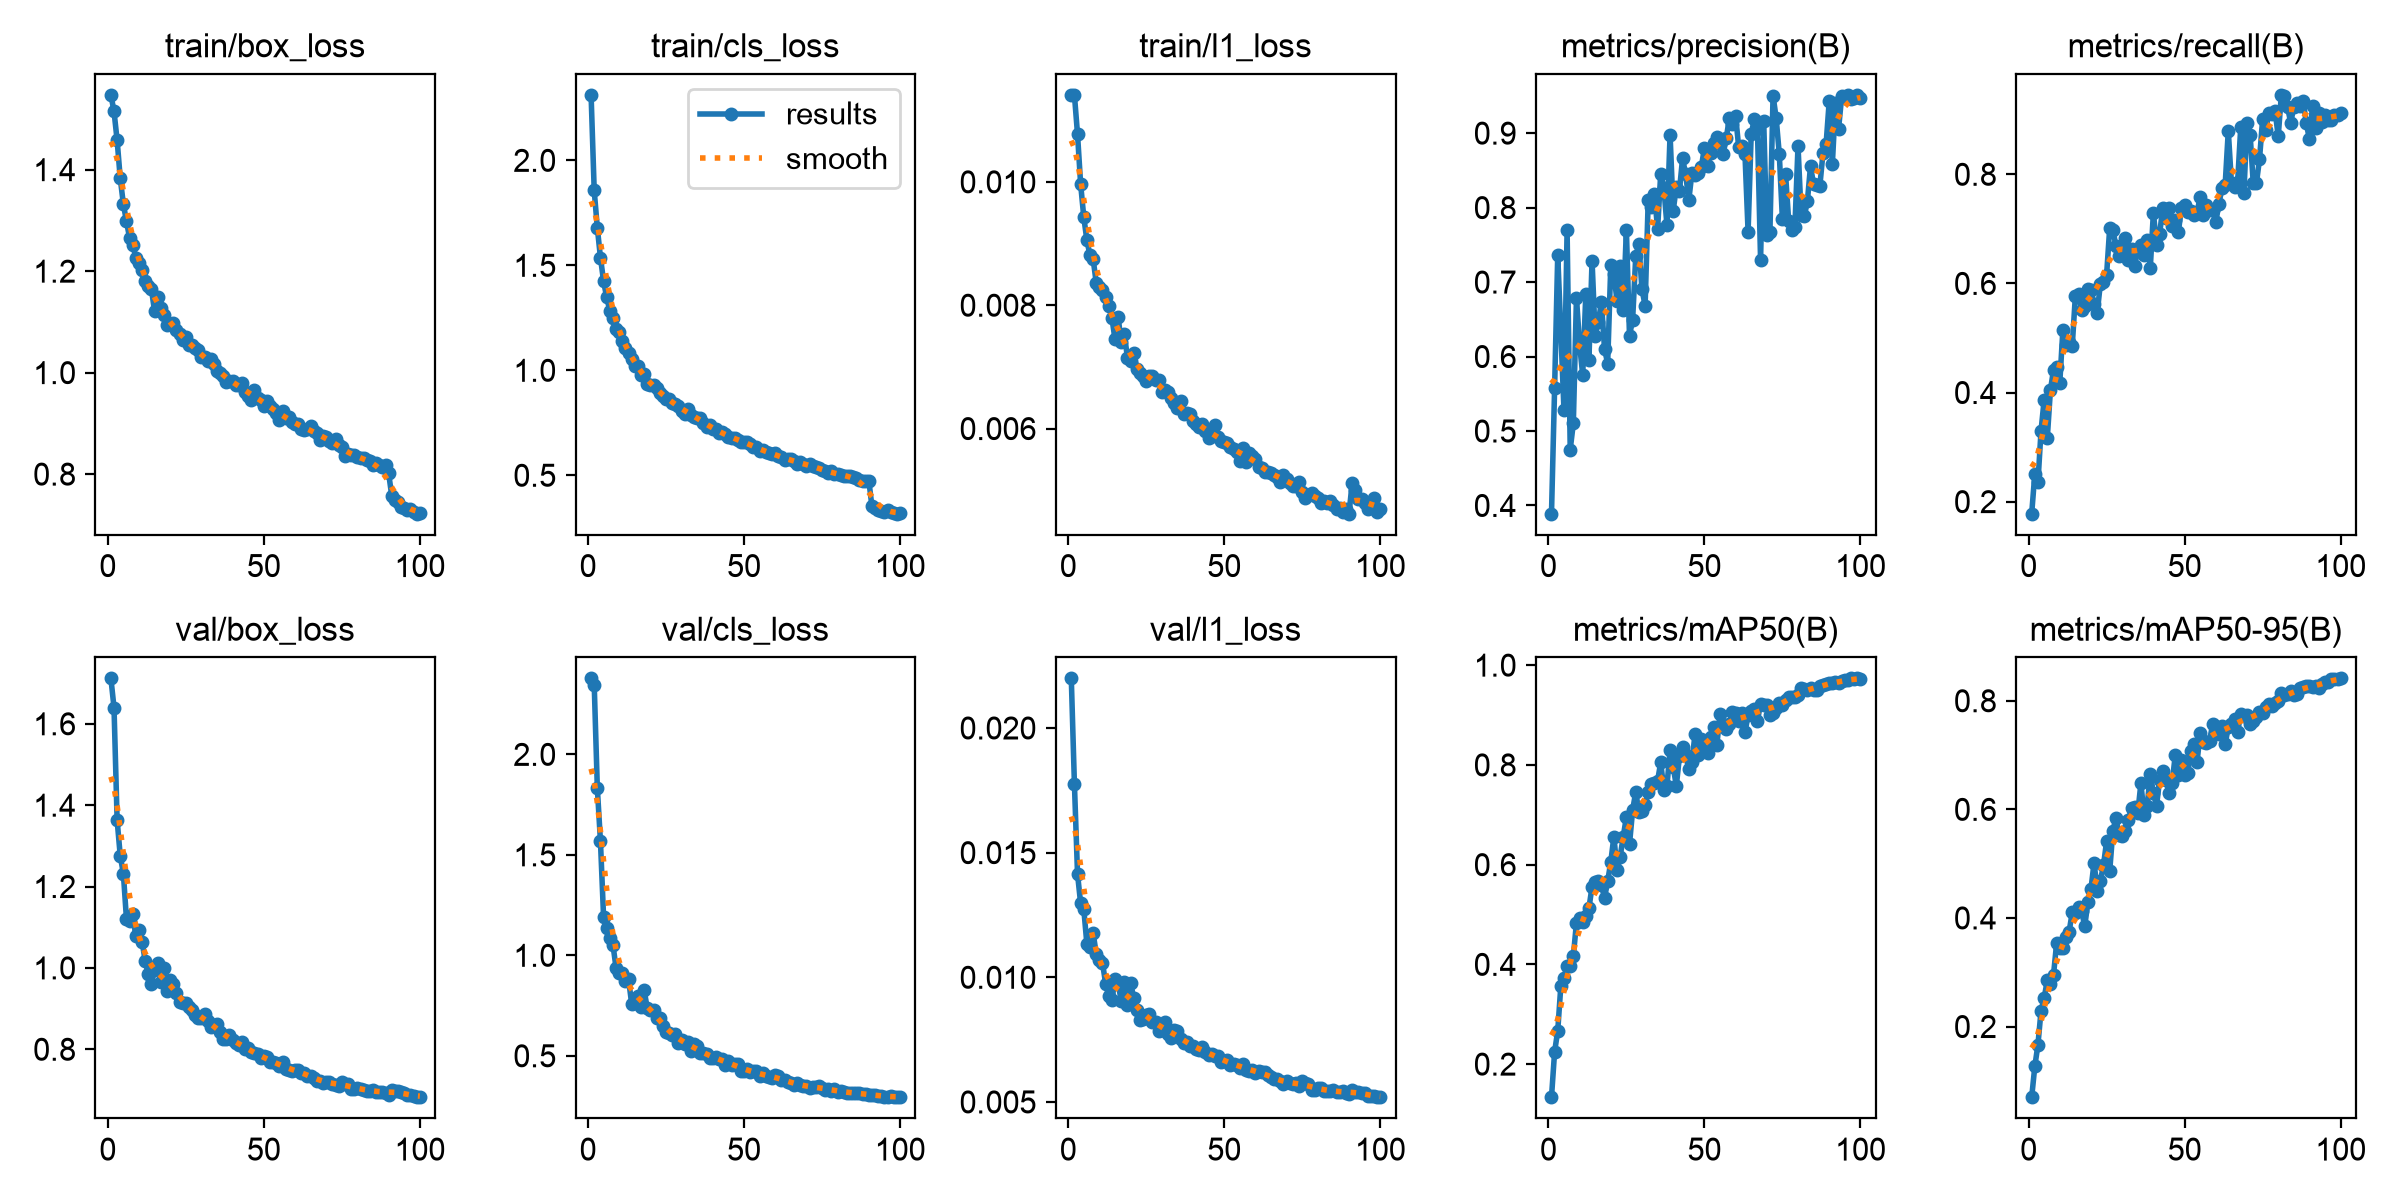
\includegraphics[width=0.92\textwidth]{results/detection/yolo26_baseline/results.png}
\caption{Accident detector training and validation history.}
\label{fig:acc-results}\end{figure}
\begin{figure}[t]\centering
\begin{minipage}{0.48\textwidth}\centering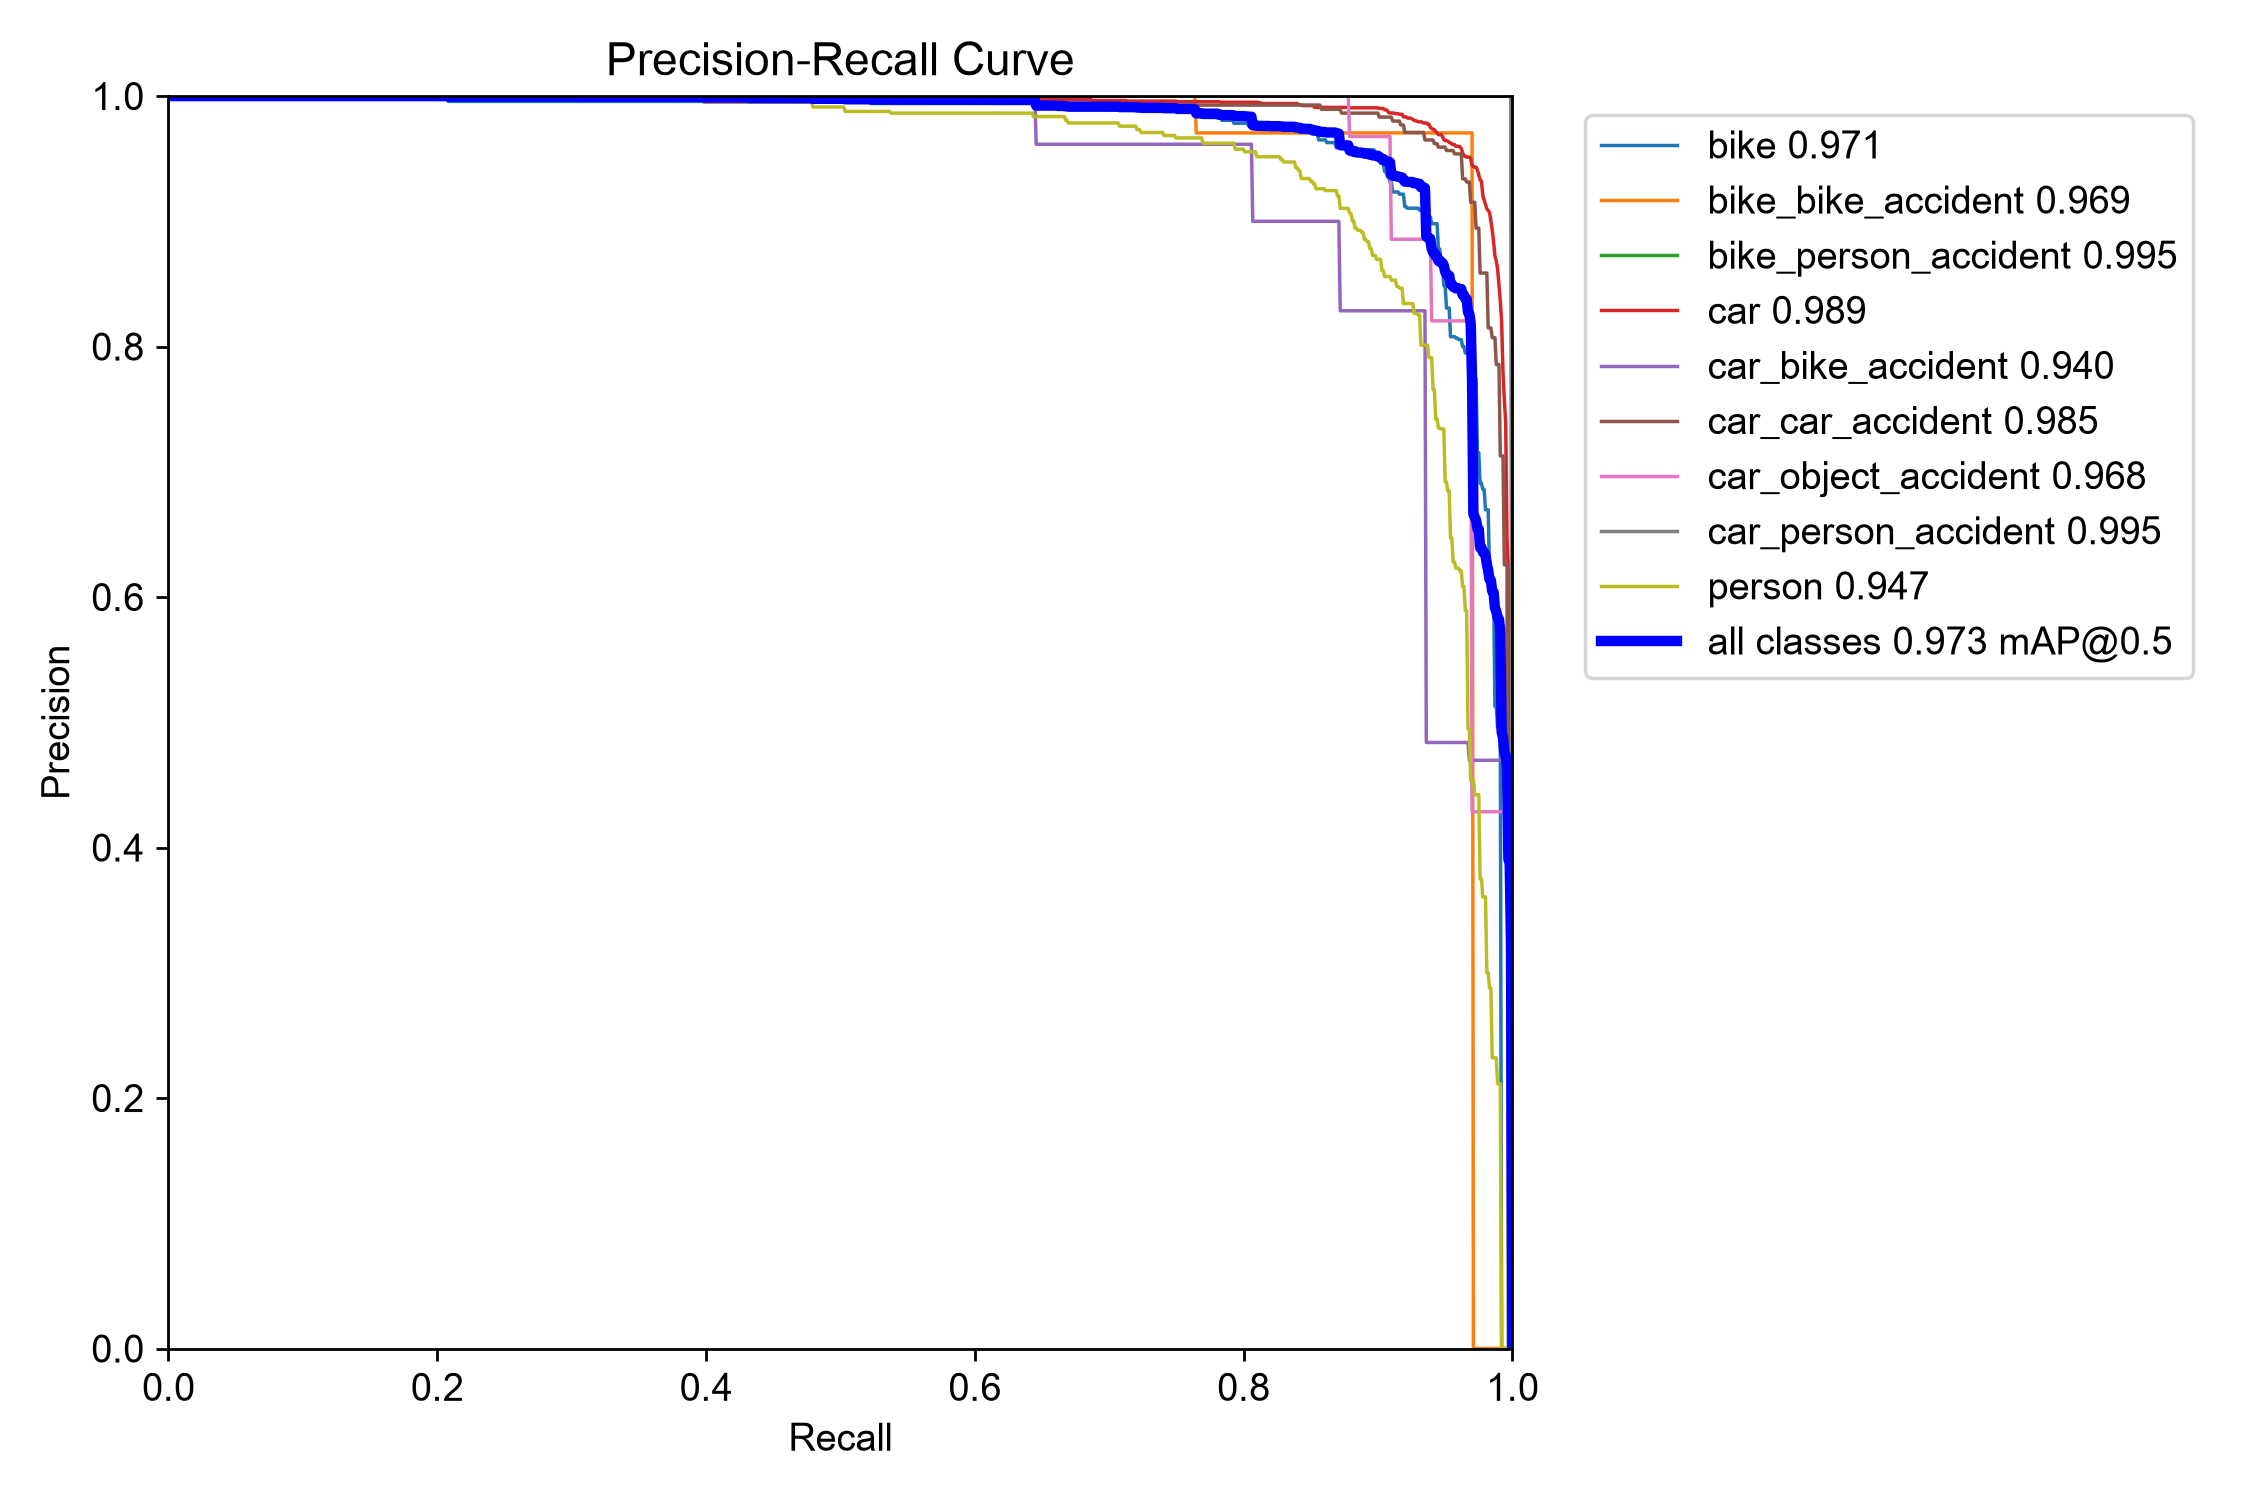
\includegraphics[width=\linewidth]{results/detection/yolo26_baseline/BoxPR_curve.png}\end{minipage}\hfill
\begin{minipage}{0.48\textwidth}\centering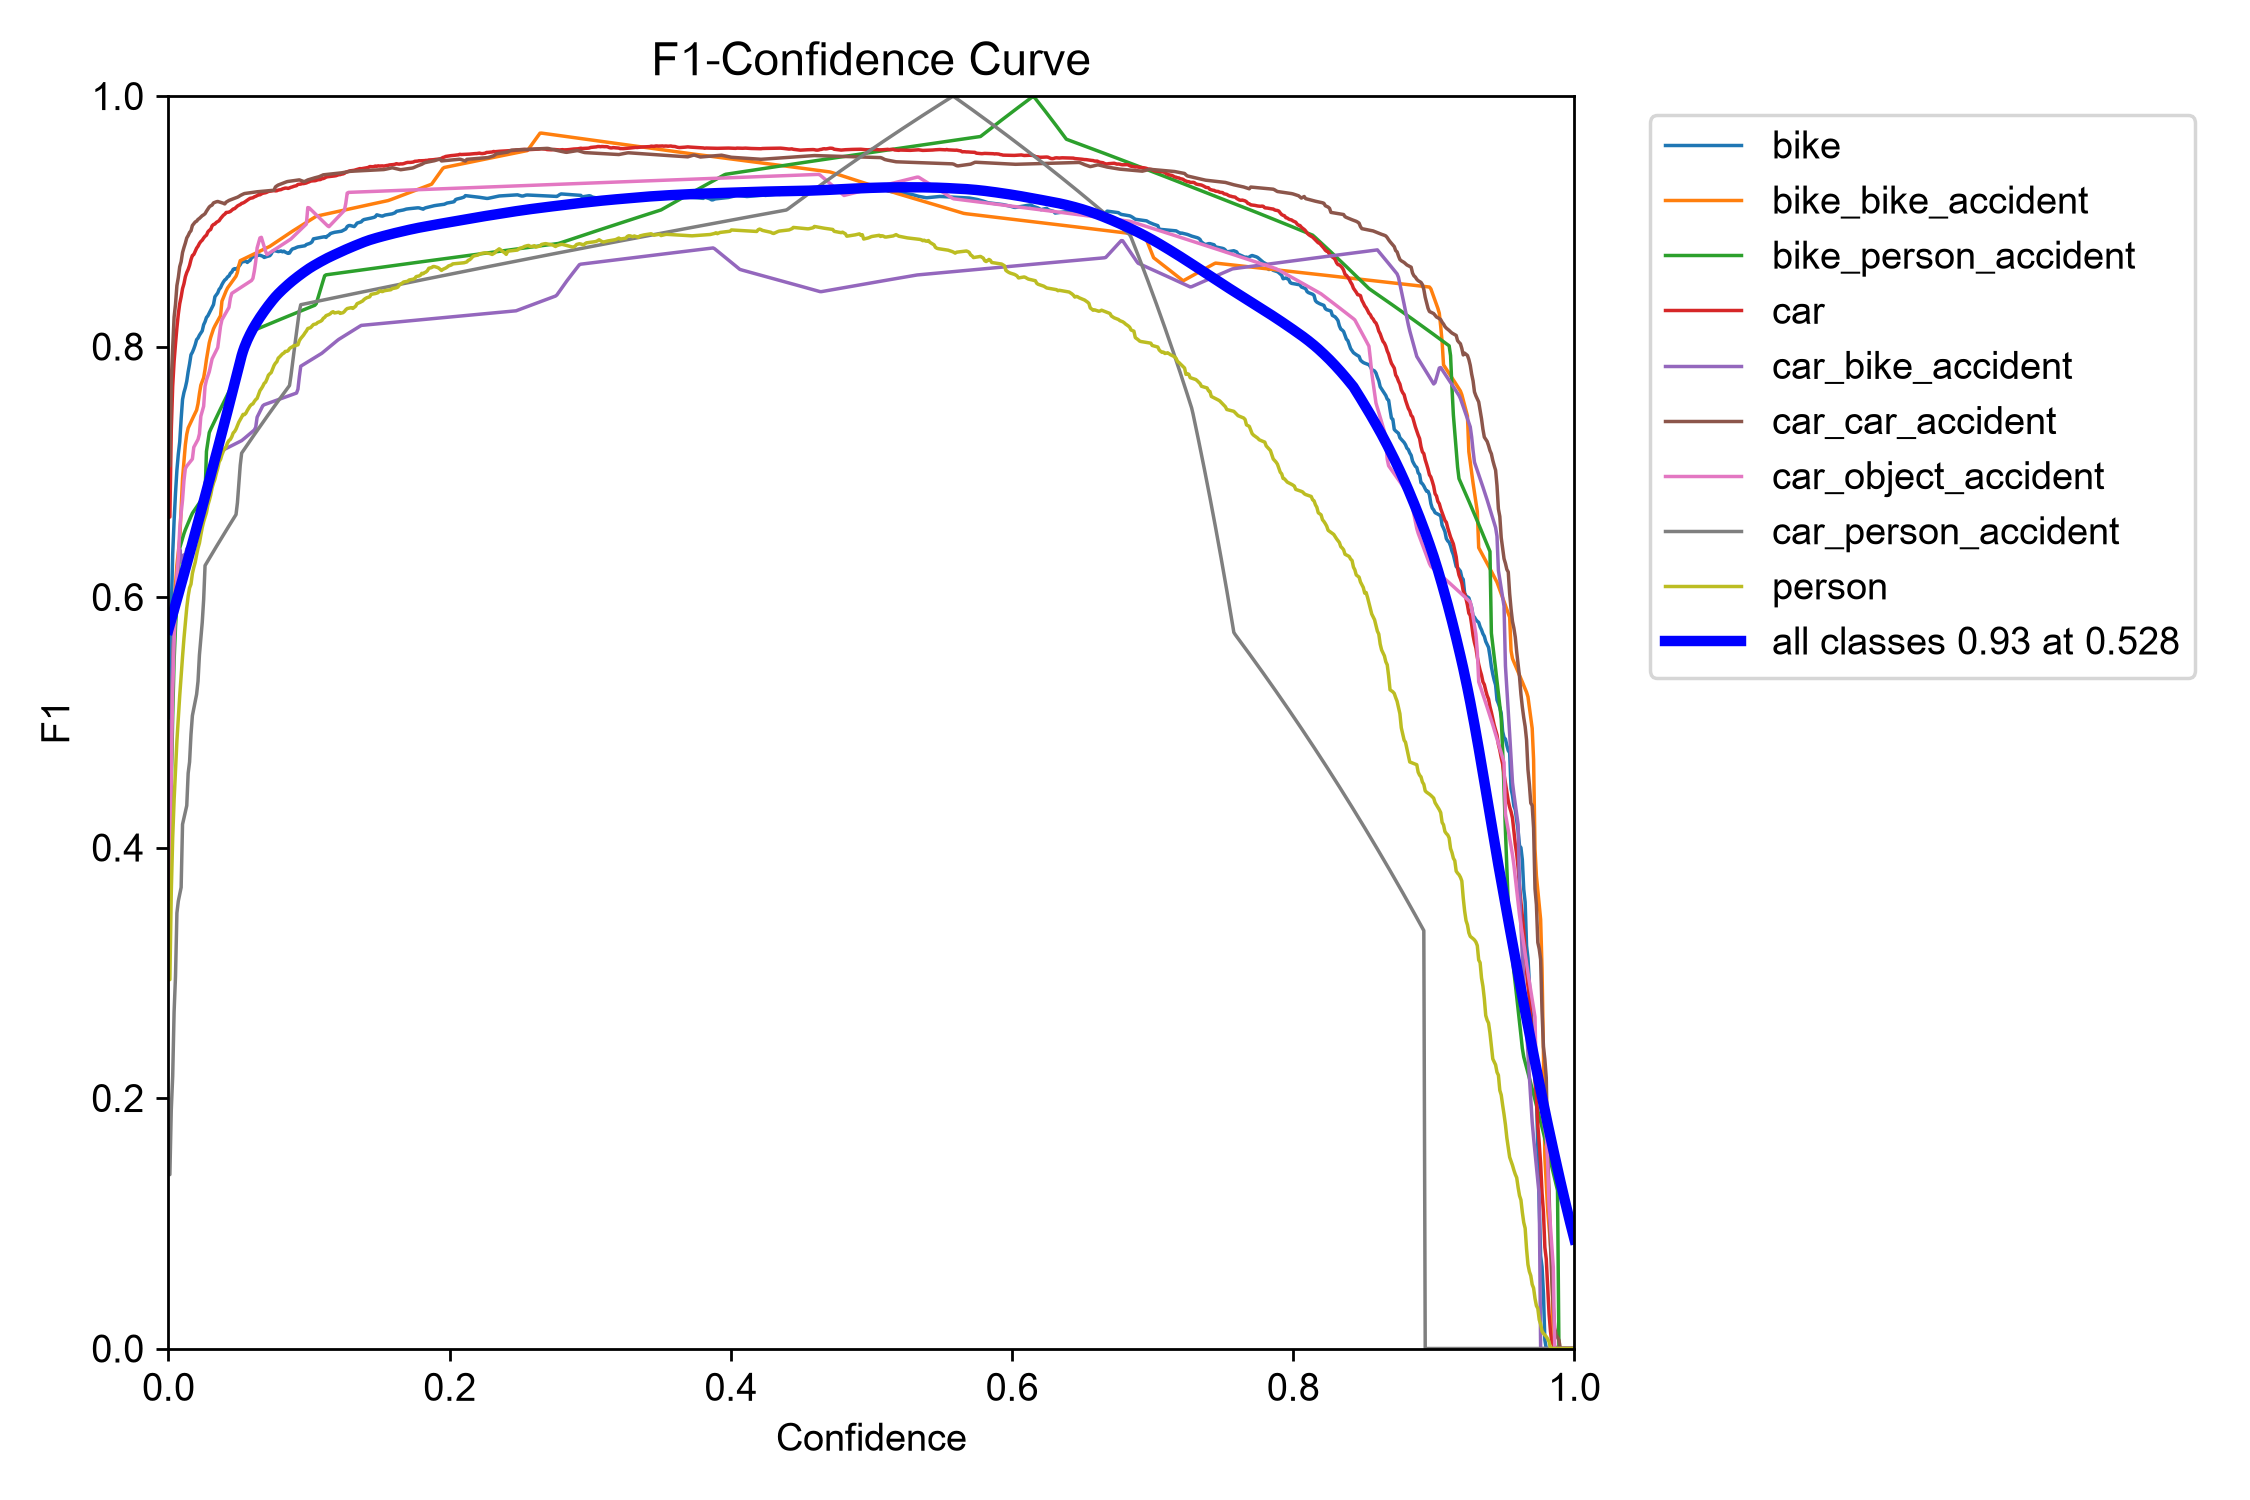
\includegraphics[width=\linewidth]{results/detection/yolo26_baseline/BoxF1_curve.png}\end{minipage}
\caption{Accident-run precision-recall and confidence-dependent F1 curves.}
\label{fig:acc-curves}\end{figure}
\begin{figure}[t]\centering
\begin{minipage}{0.48\textwidth}\centering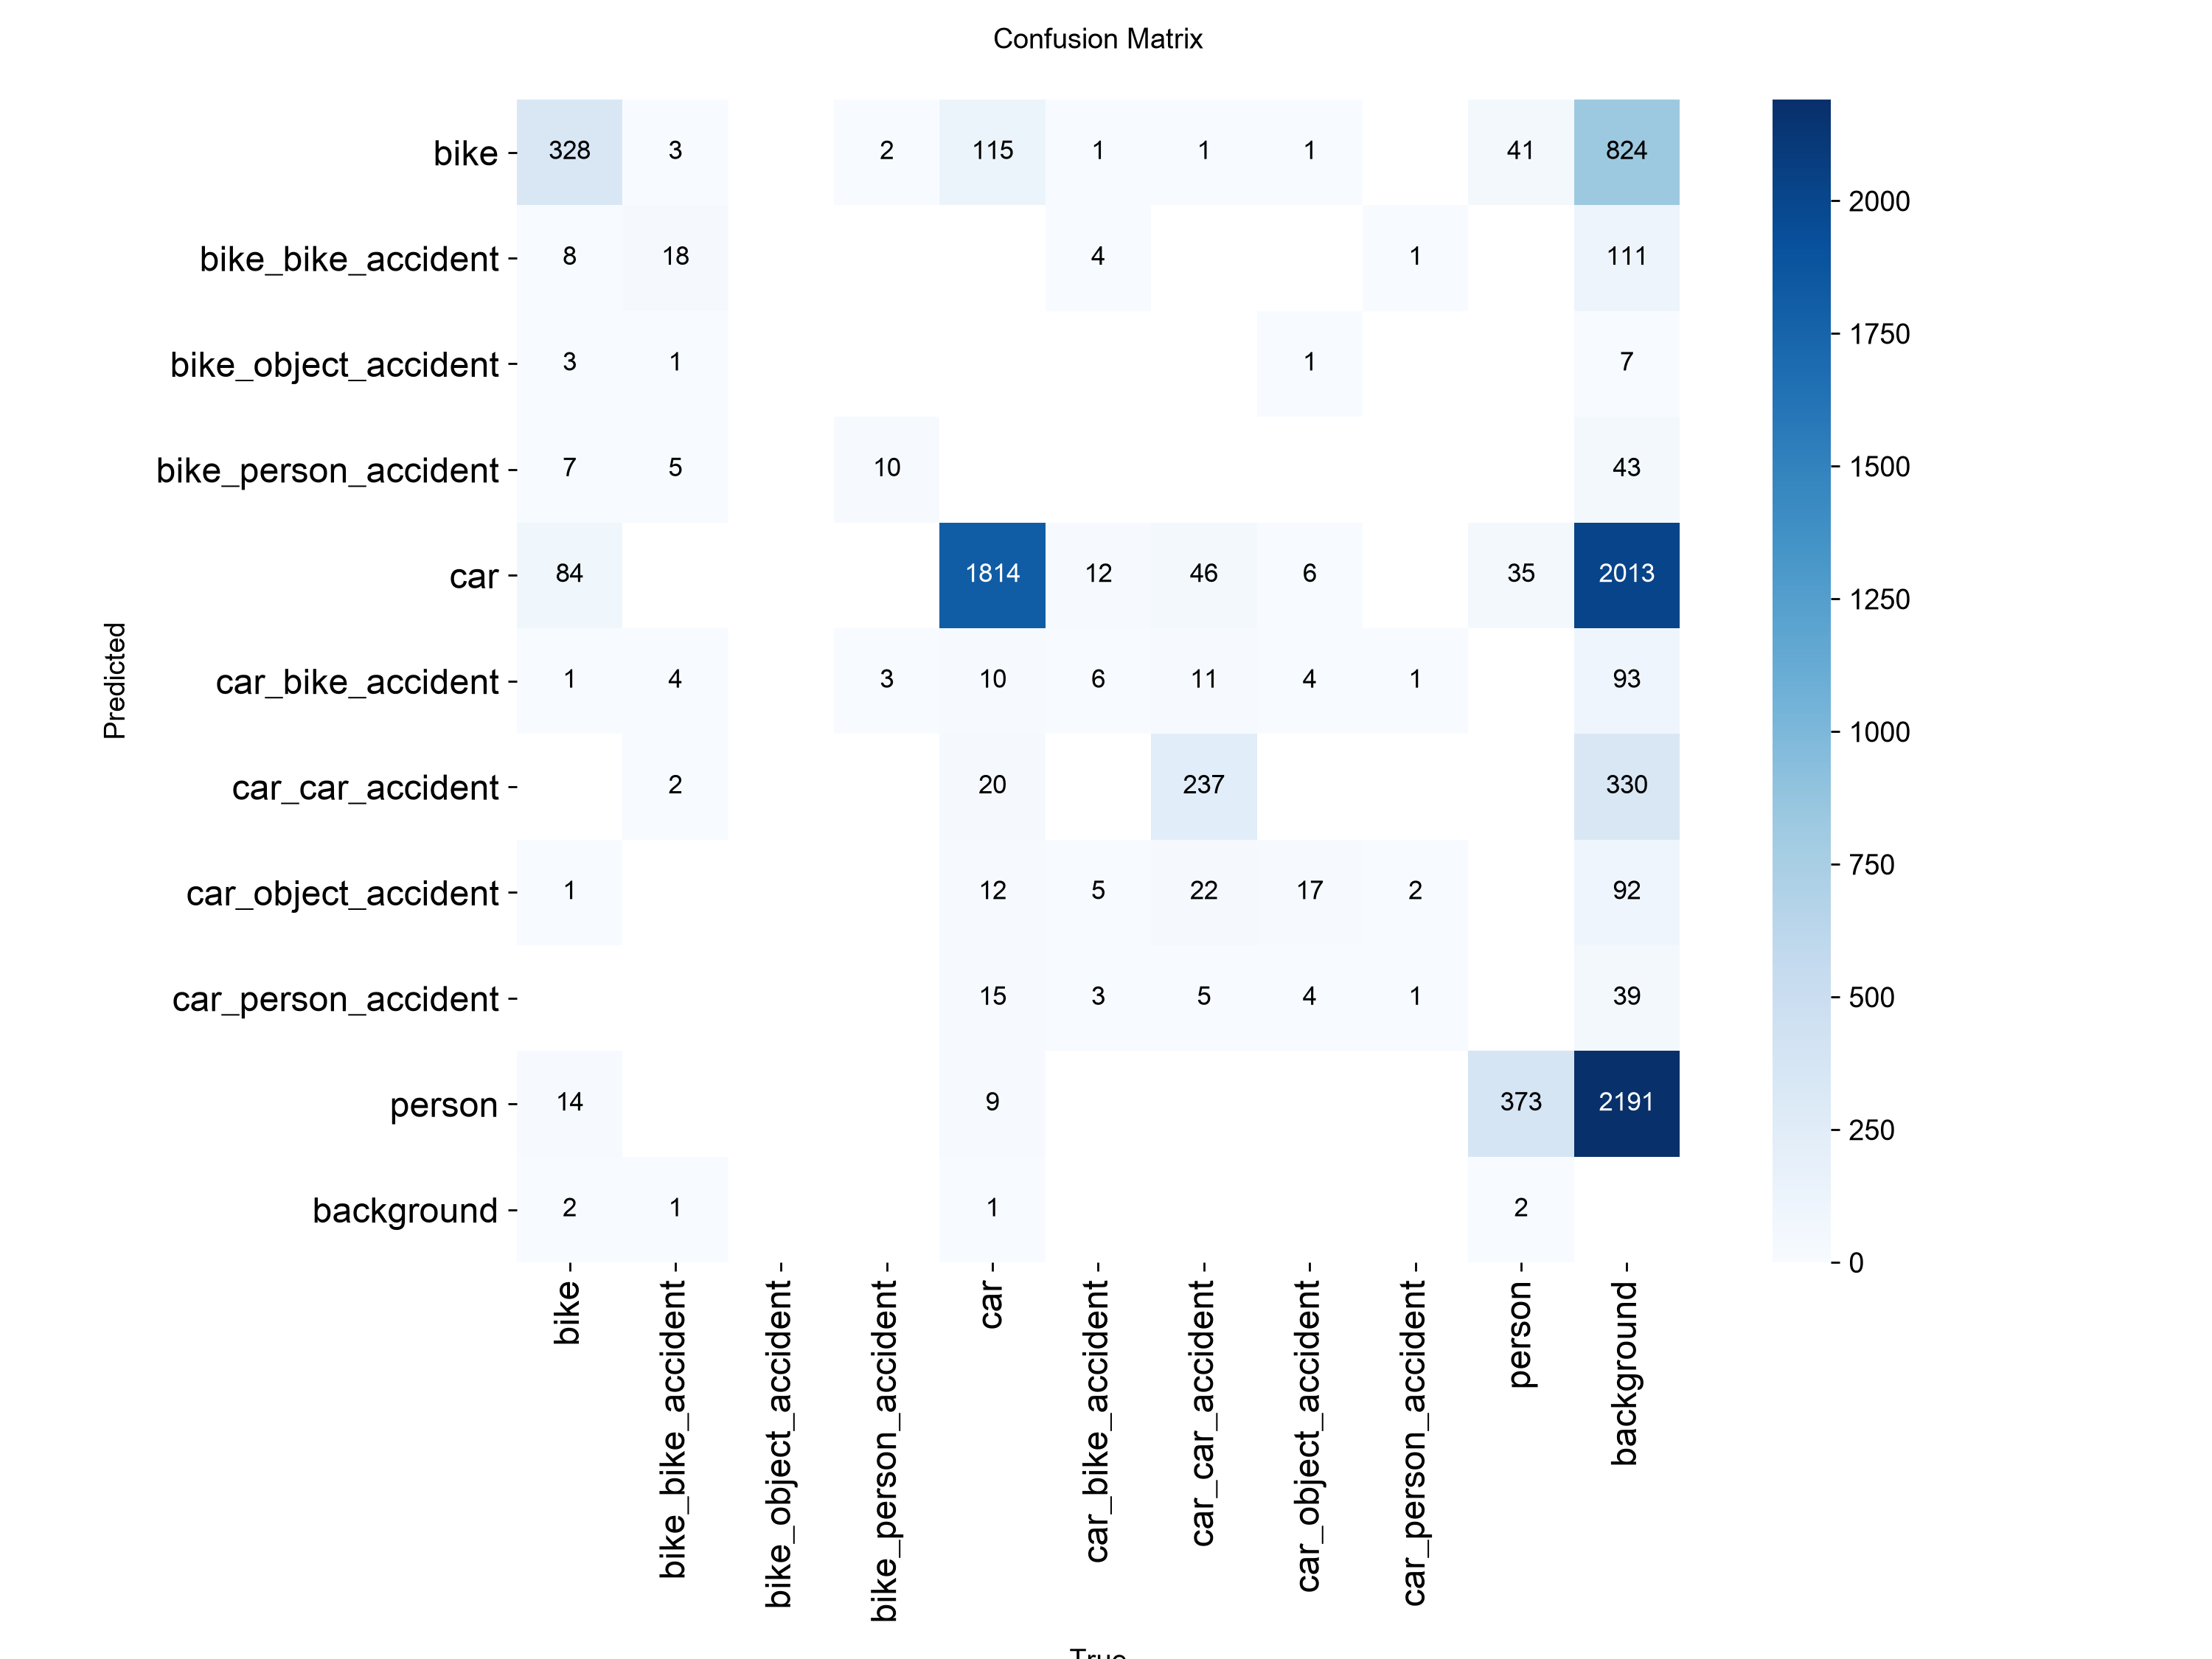
\includegraphics[width=\linewidth]{results/detection/yolo26_baseline/confusion_matrix.png}\end{minipage}\hfill
\begin{minipage}{0.48\textwidth}\centering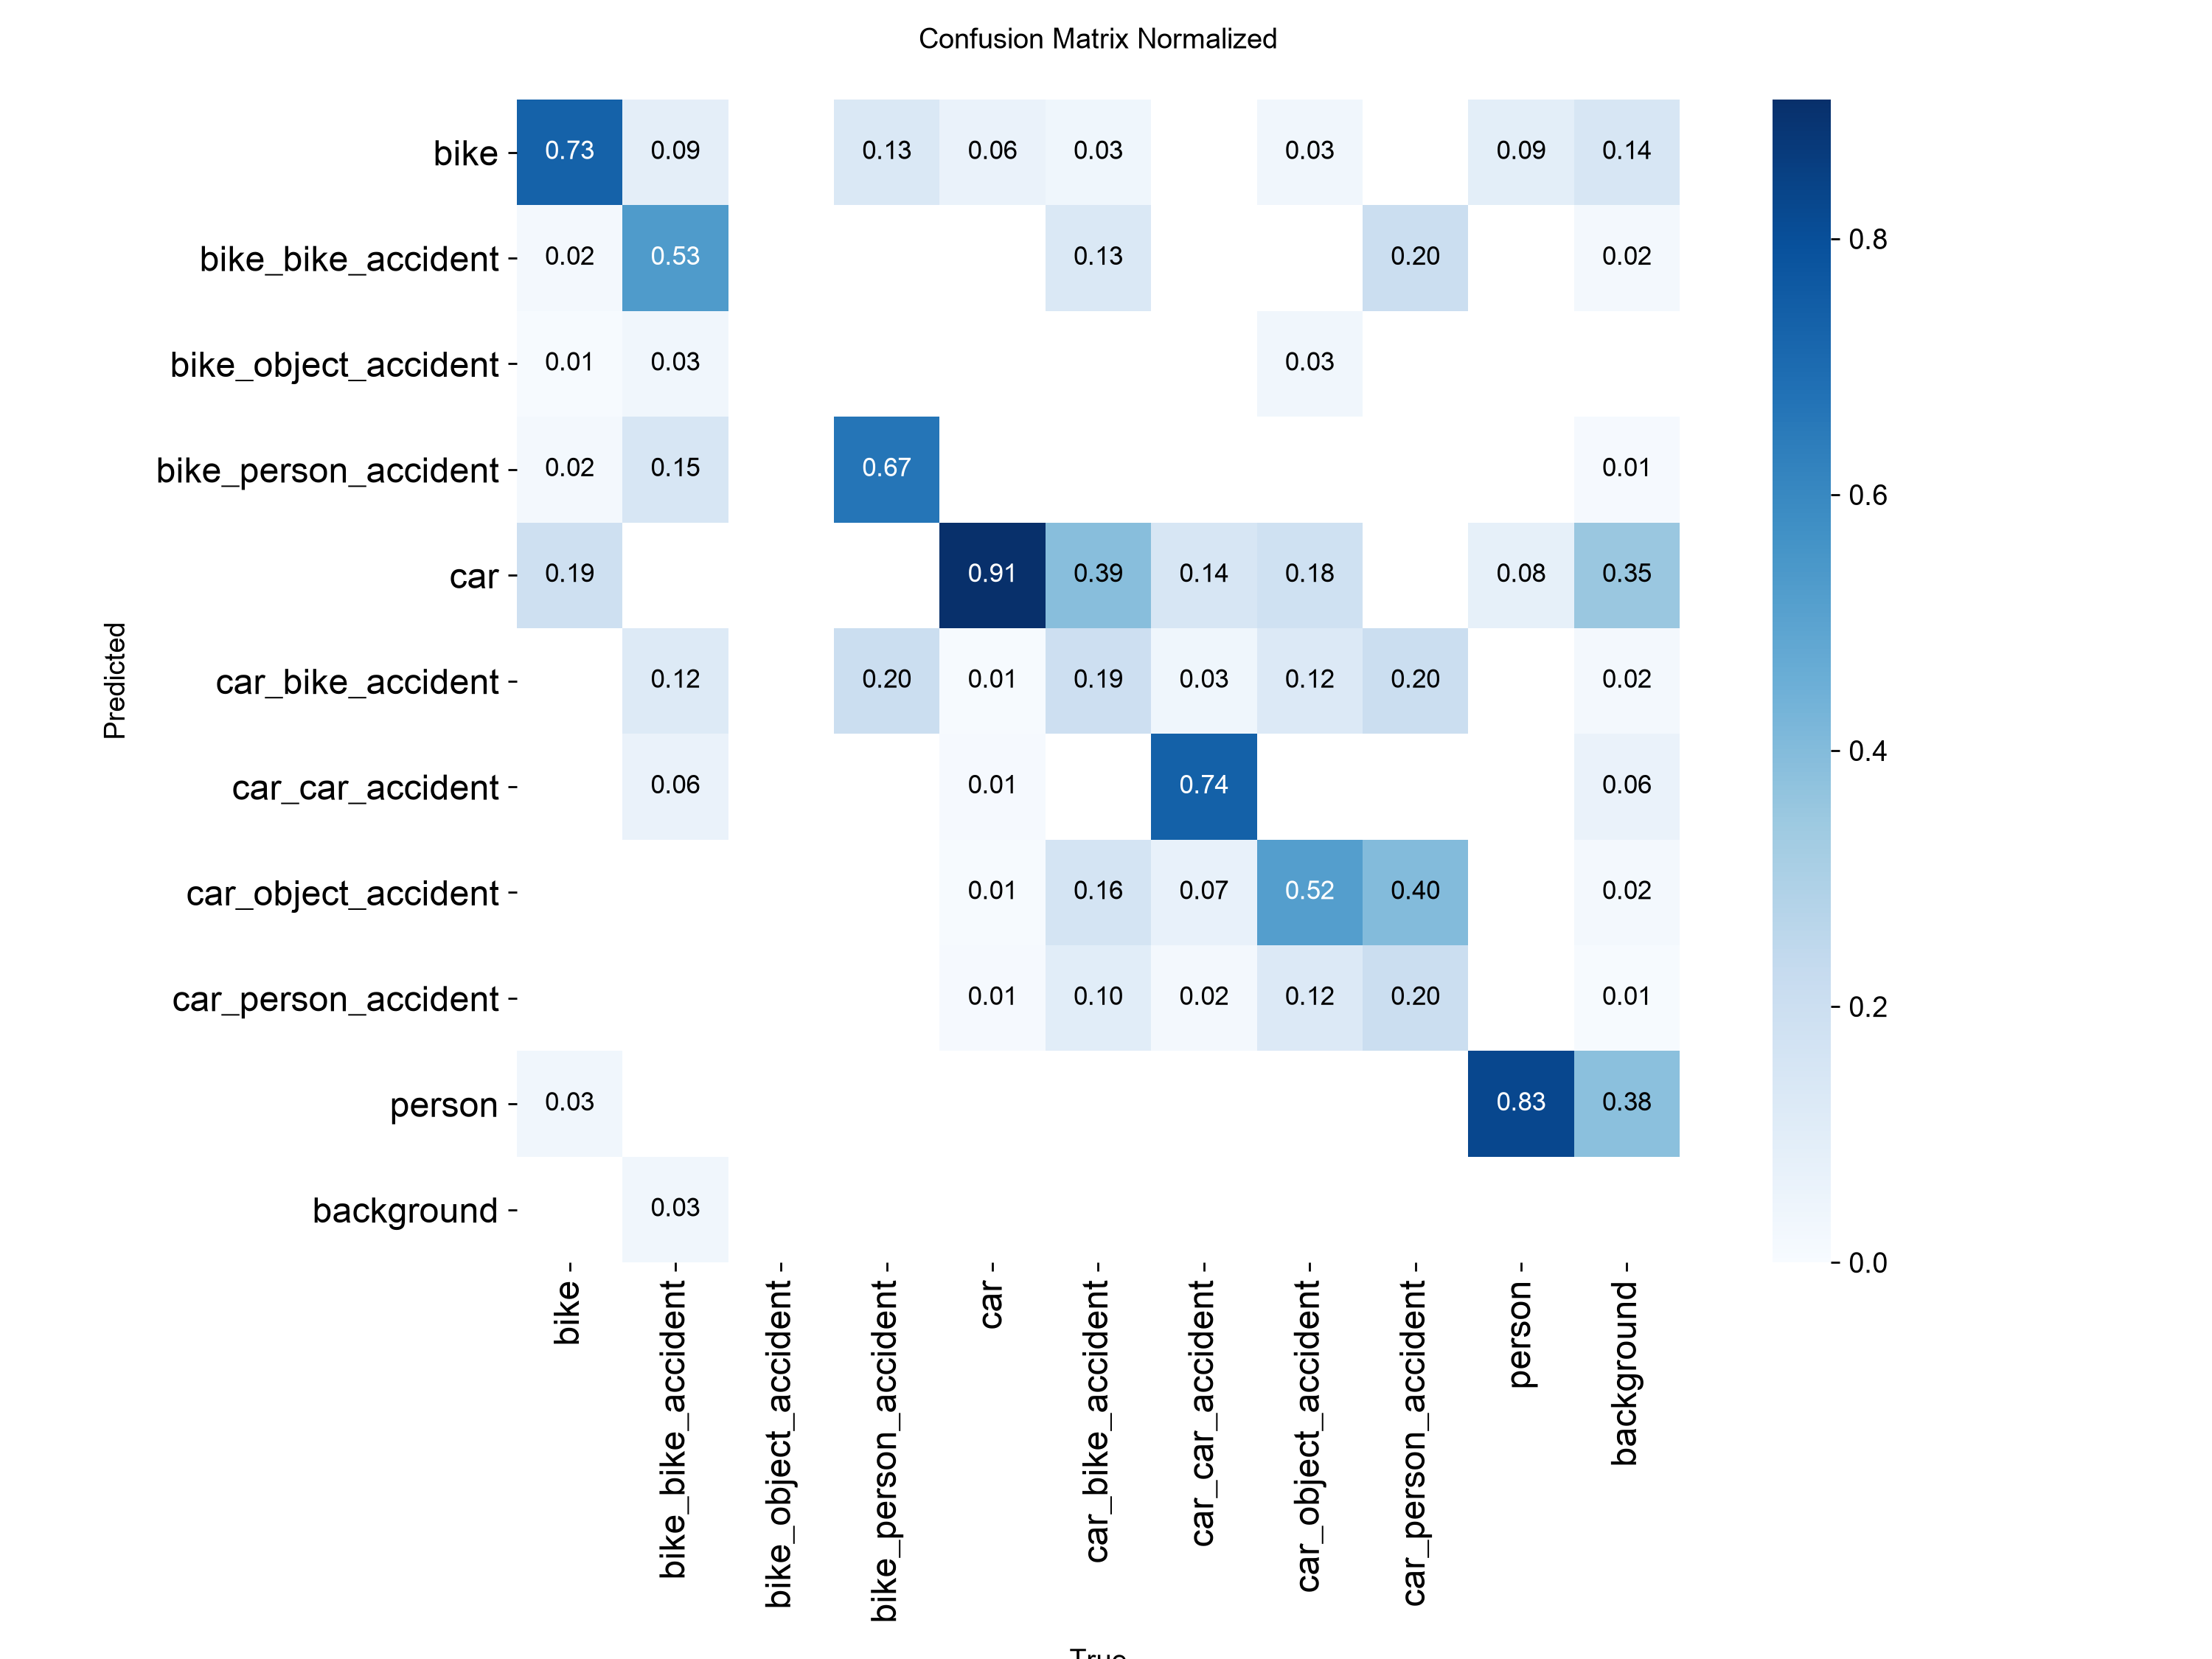
\includegraphics[width=\linewidth]{results/detection/yolo26_baseline/confusion_matrix_normalized.png}\end{minipage}
\caption{Raw and normalized accident-run confusion matrices.}
\label{fig:acc-conf}\end{figure}

The PR plot displays AP@0.5 for nine classes; bike--object is not listed. Confusion-matrix cells show errors obscured by an aggregate average, particularly for classes with few examples and for interaction labels confused with ordinary objects. Counts and confusion patterns should therefore accompany aggregate AP. The mAP@0.5 to mAP@0.5:0.95 difference is 13.20 percentage points, consistent with more stringent localization criteria but insufficient to diagnose the error source.

The severity validation run's final values are 76.174\% precision, 77.897\% recall, 82.157\% mAP@0.5, and 60.530\% mAP@0.5:0.95. The best validation summary records approximately 80.20\%, 75.20\%, 82.52\%, and 60.62\%, respectively. Metric-specific best epochs differ. The severity run's best logged precision is 83.228\% at epoch 95; best recall is 77.897\% at epoch 100; best mAP@0.5 is 82.521\% at epoch 96; and best mAP@0.5:0.95 is 60.692\% at epoch 99. Its final row is lower than the metric-specific best for three measures. These values should remain associated with their actual epochs, and future reporting should name the single checkpoint used for all test evaluation.
The separate test summary reports 79.74\% precision, 71.81\% recall, 80.45\% mAP@0.5, and 55.47\% mAP@0.5:0.95. Per-class test precision/recall/AP@0.5 are moderate-accident 76.42/74.65/81.39\%, no-accident 80.45/70.30/81.43\%, and severe-accident 82.36/70.50/78.54\%. These results describe detection labels in the saved evaluation; they do not establish medical injury classification.

Severity annotations comprise 9,408 boxes: 19.75\% moderate, 50.67\% no-accident, and 29.58\% severe. The data-inspection report found seven unusually large boxes but no missing images or labels, empty labels, invalid IDs, invalid formats, or out-of-bounds boxes in that inspection. This checks file structure, not semantic truth. A severity rubric, class-wise confusion table, and assessment against a suitable independent reference remain necessary.

\begin{figure}[t]\centering
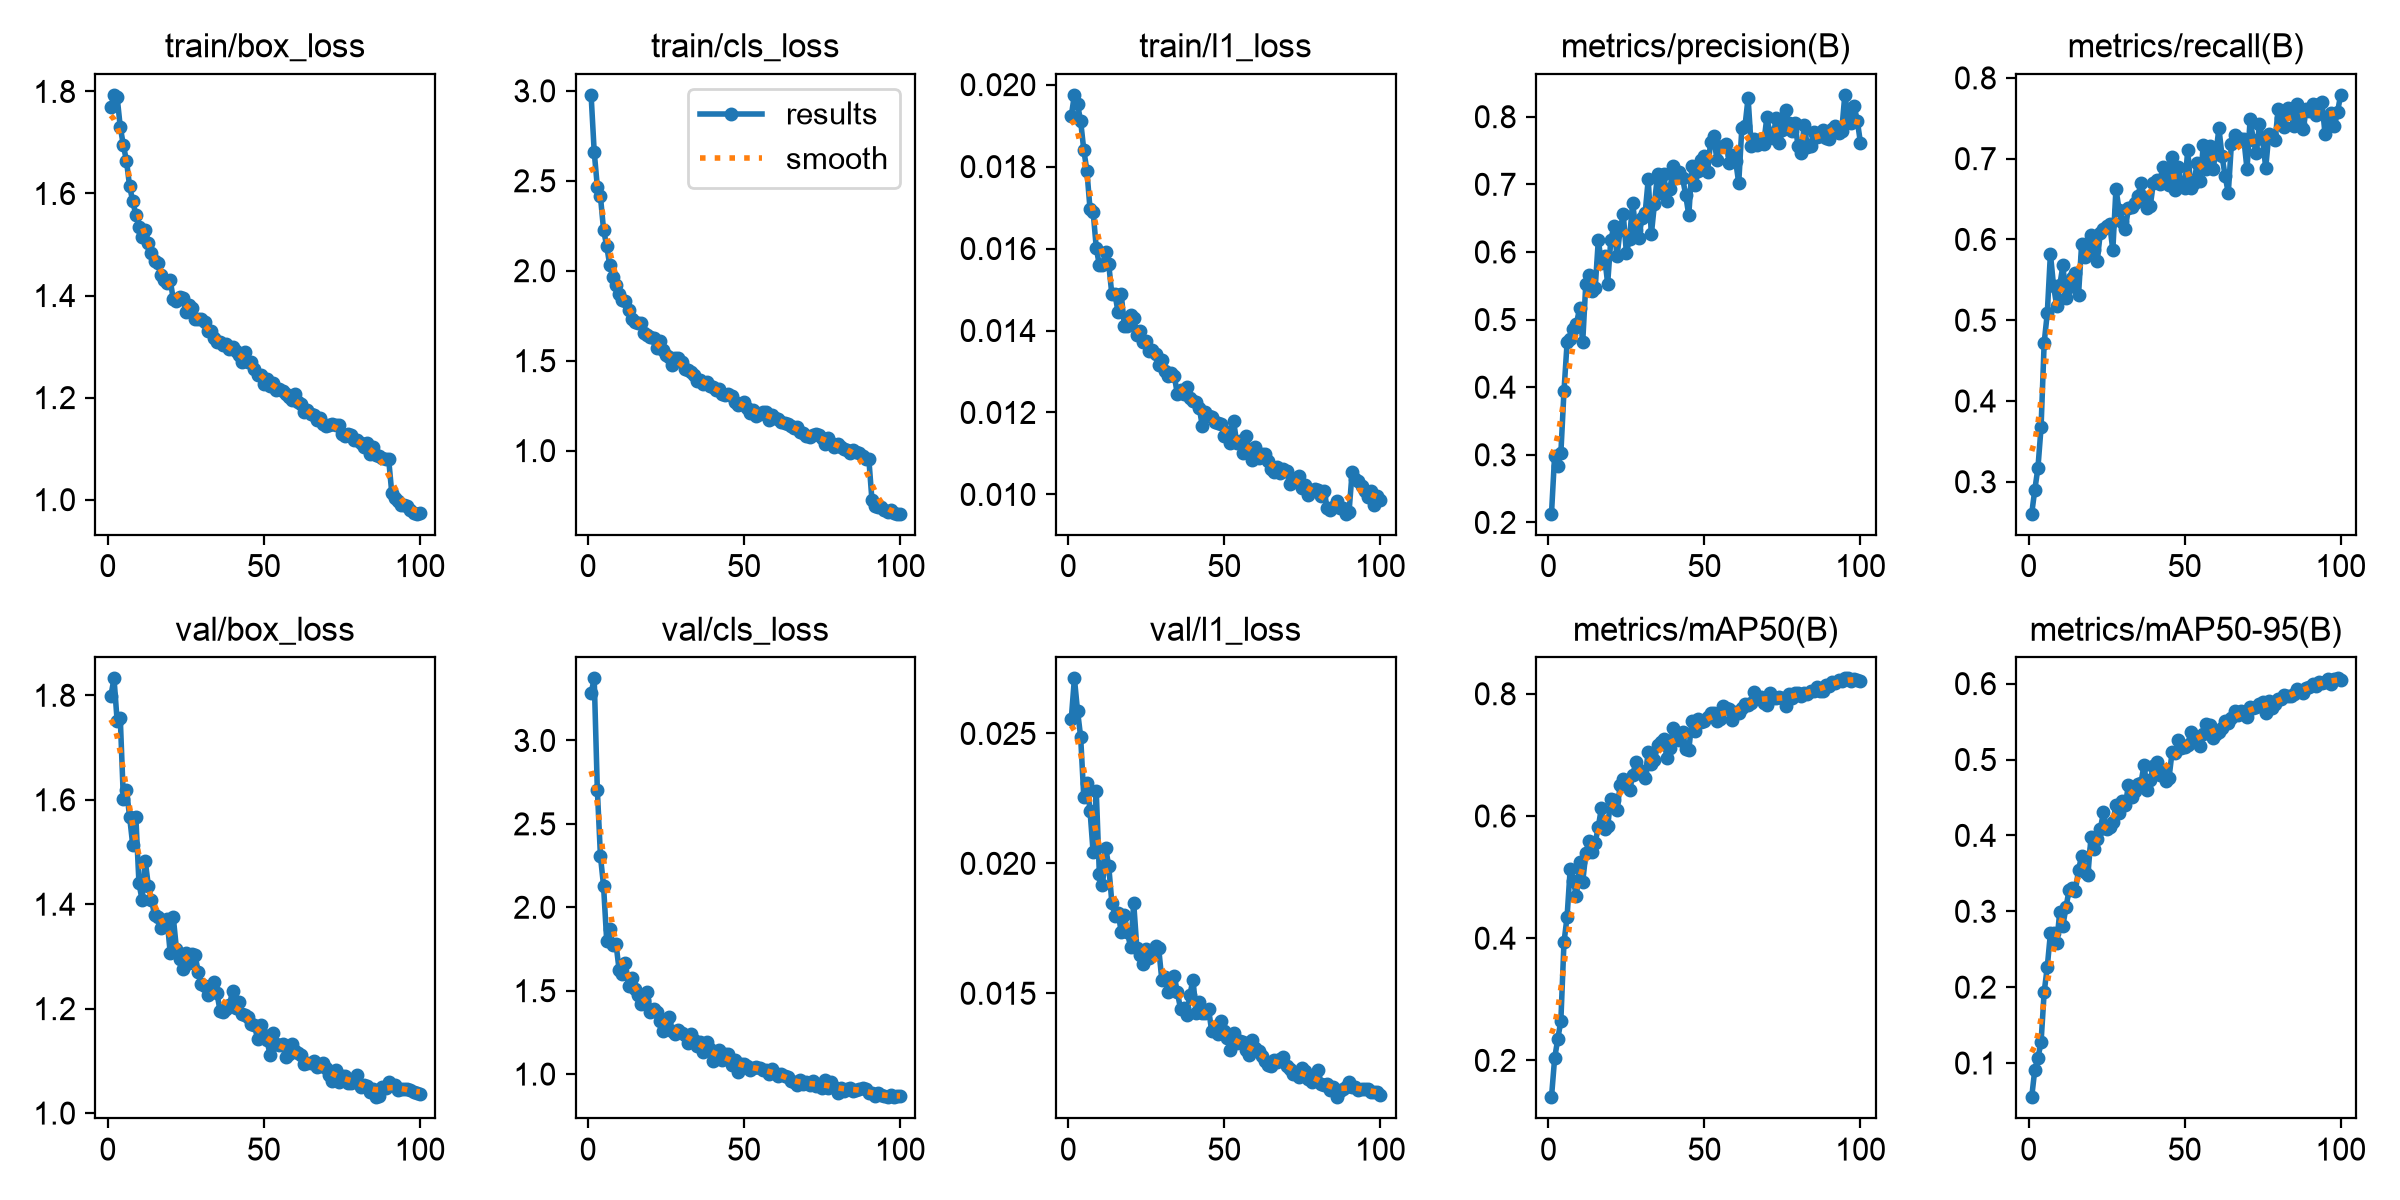
\includegraphics[width=0.92\textwidth]{results/detection/accident_severity-2/results.png}
\caption{Severity-model training and validation history.}
\label{fig:sev-results}\end{figure}
\begin{figure}[t]\centering
\begin{minipage}{0.48\textwidth}\centering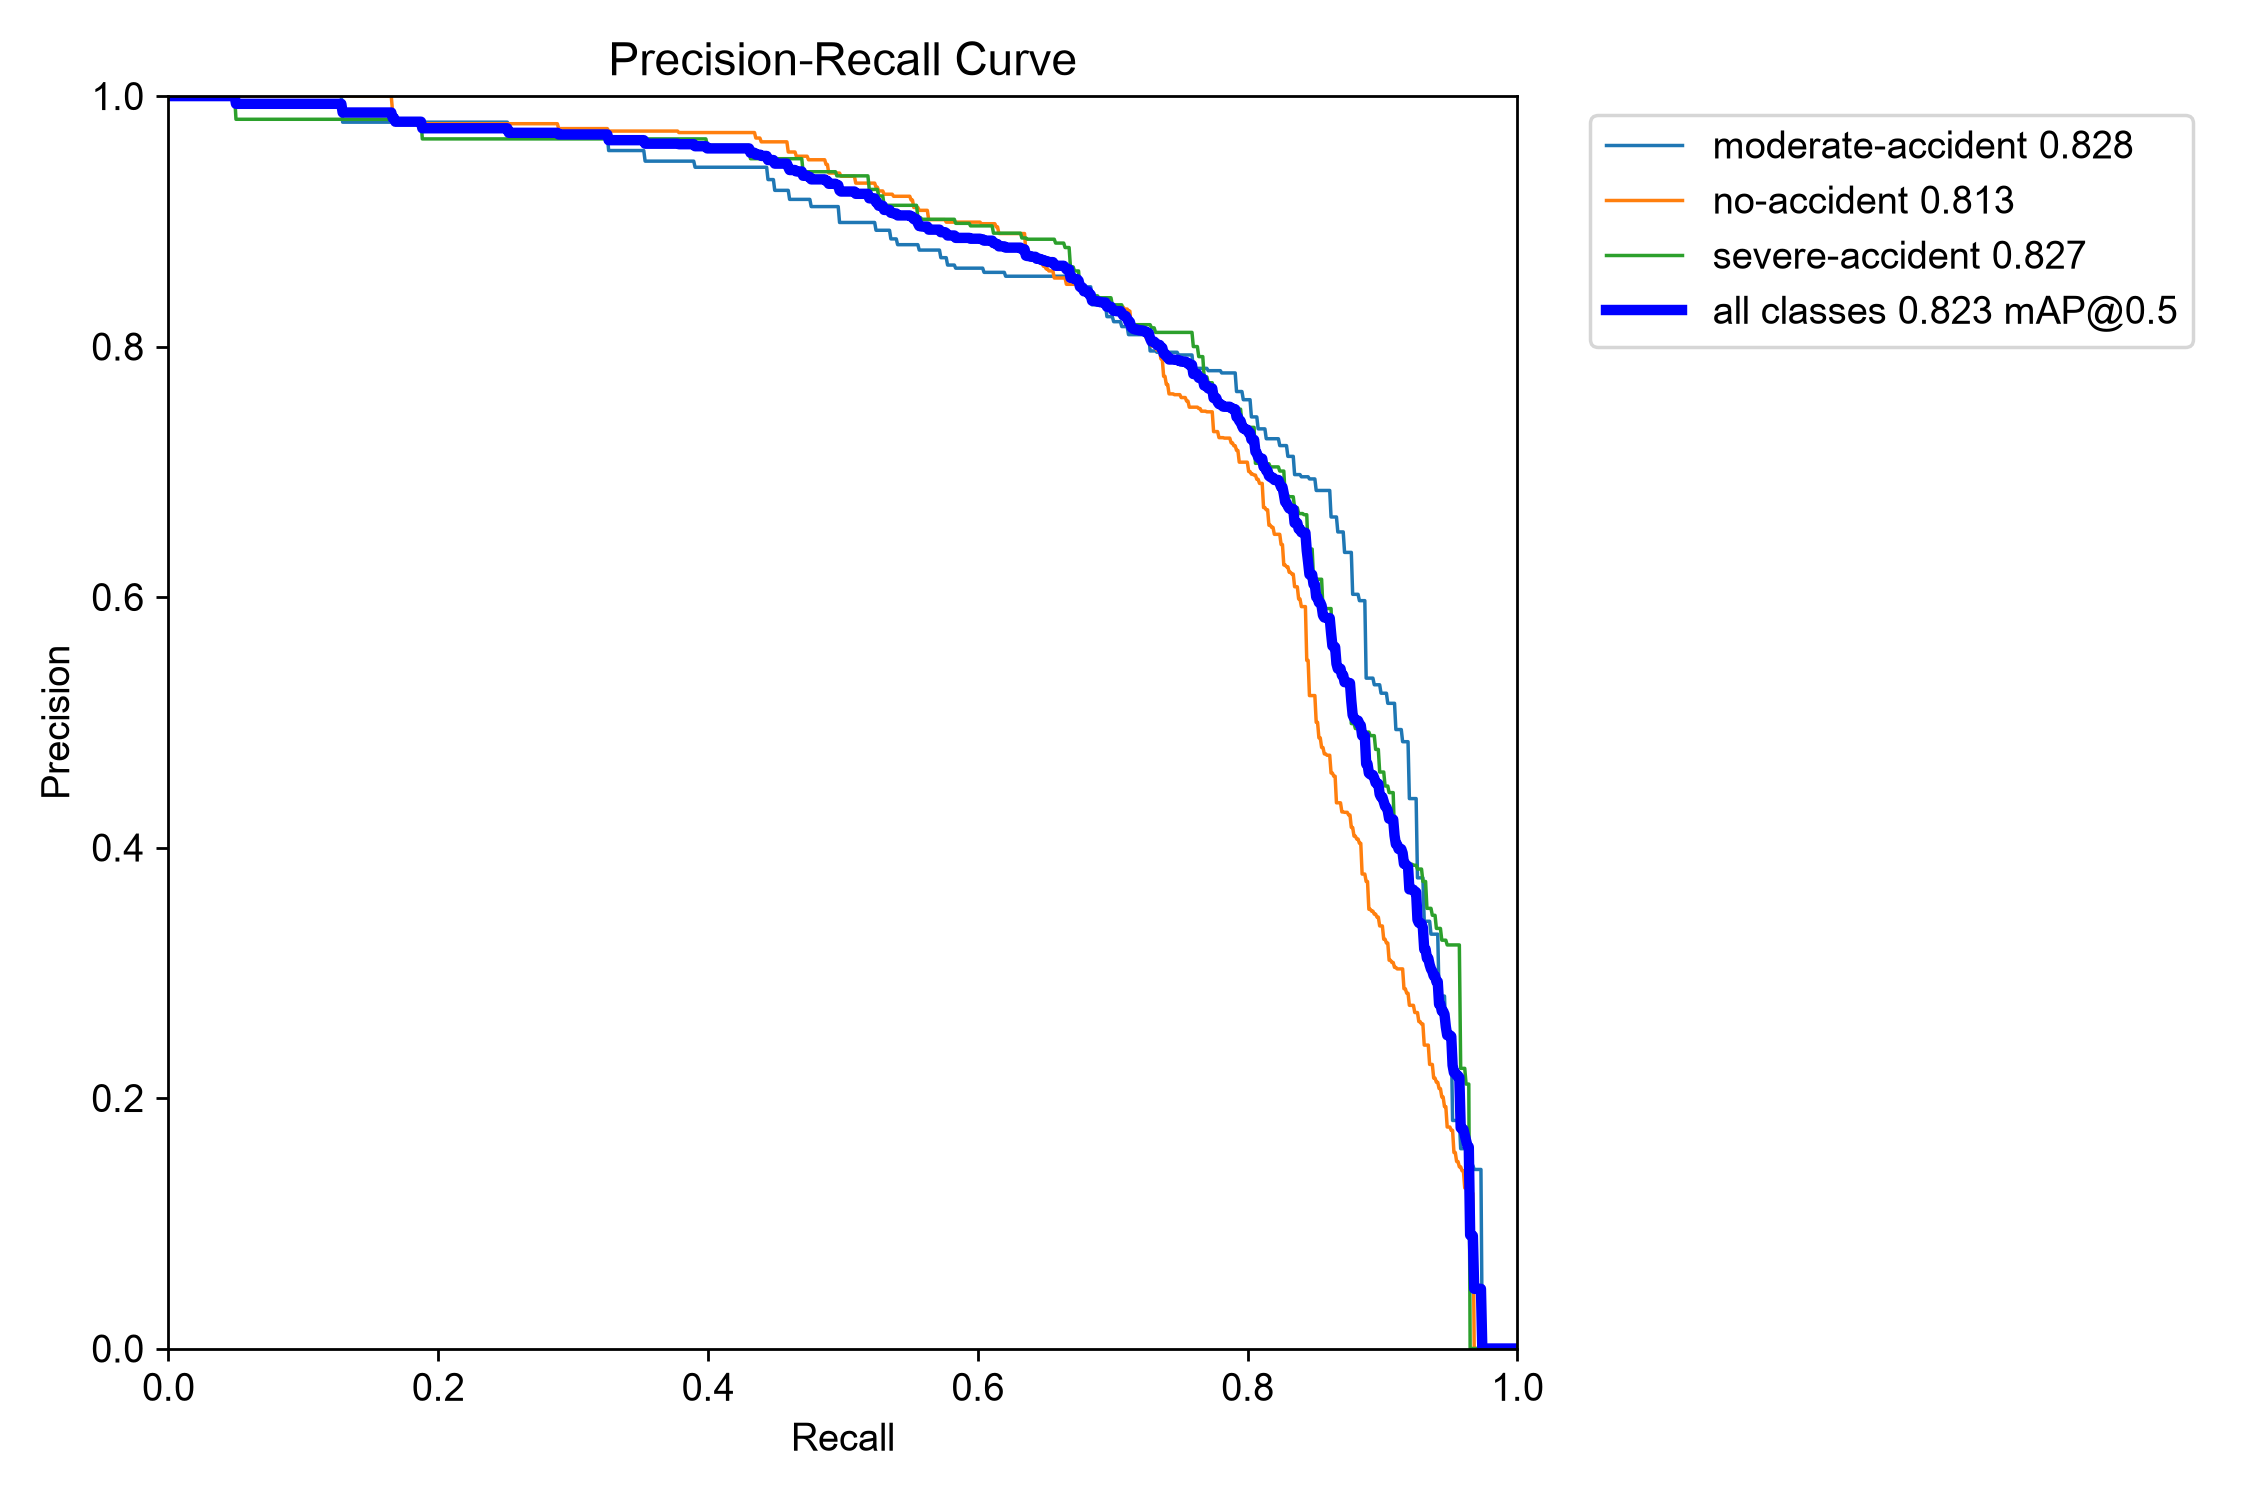
\includegraphics[width=\linewidth]{results/detection/accident_severity-2/BoxPR_curve.png}\end{minipage}\hfill
\begin{minipage}{0.48\textwidth}\centering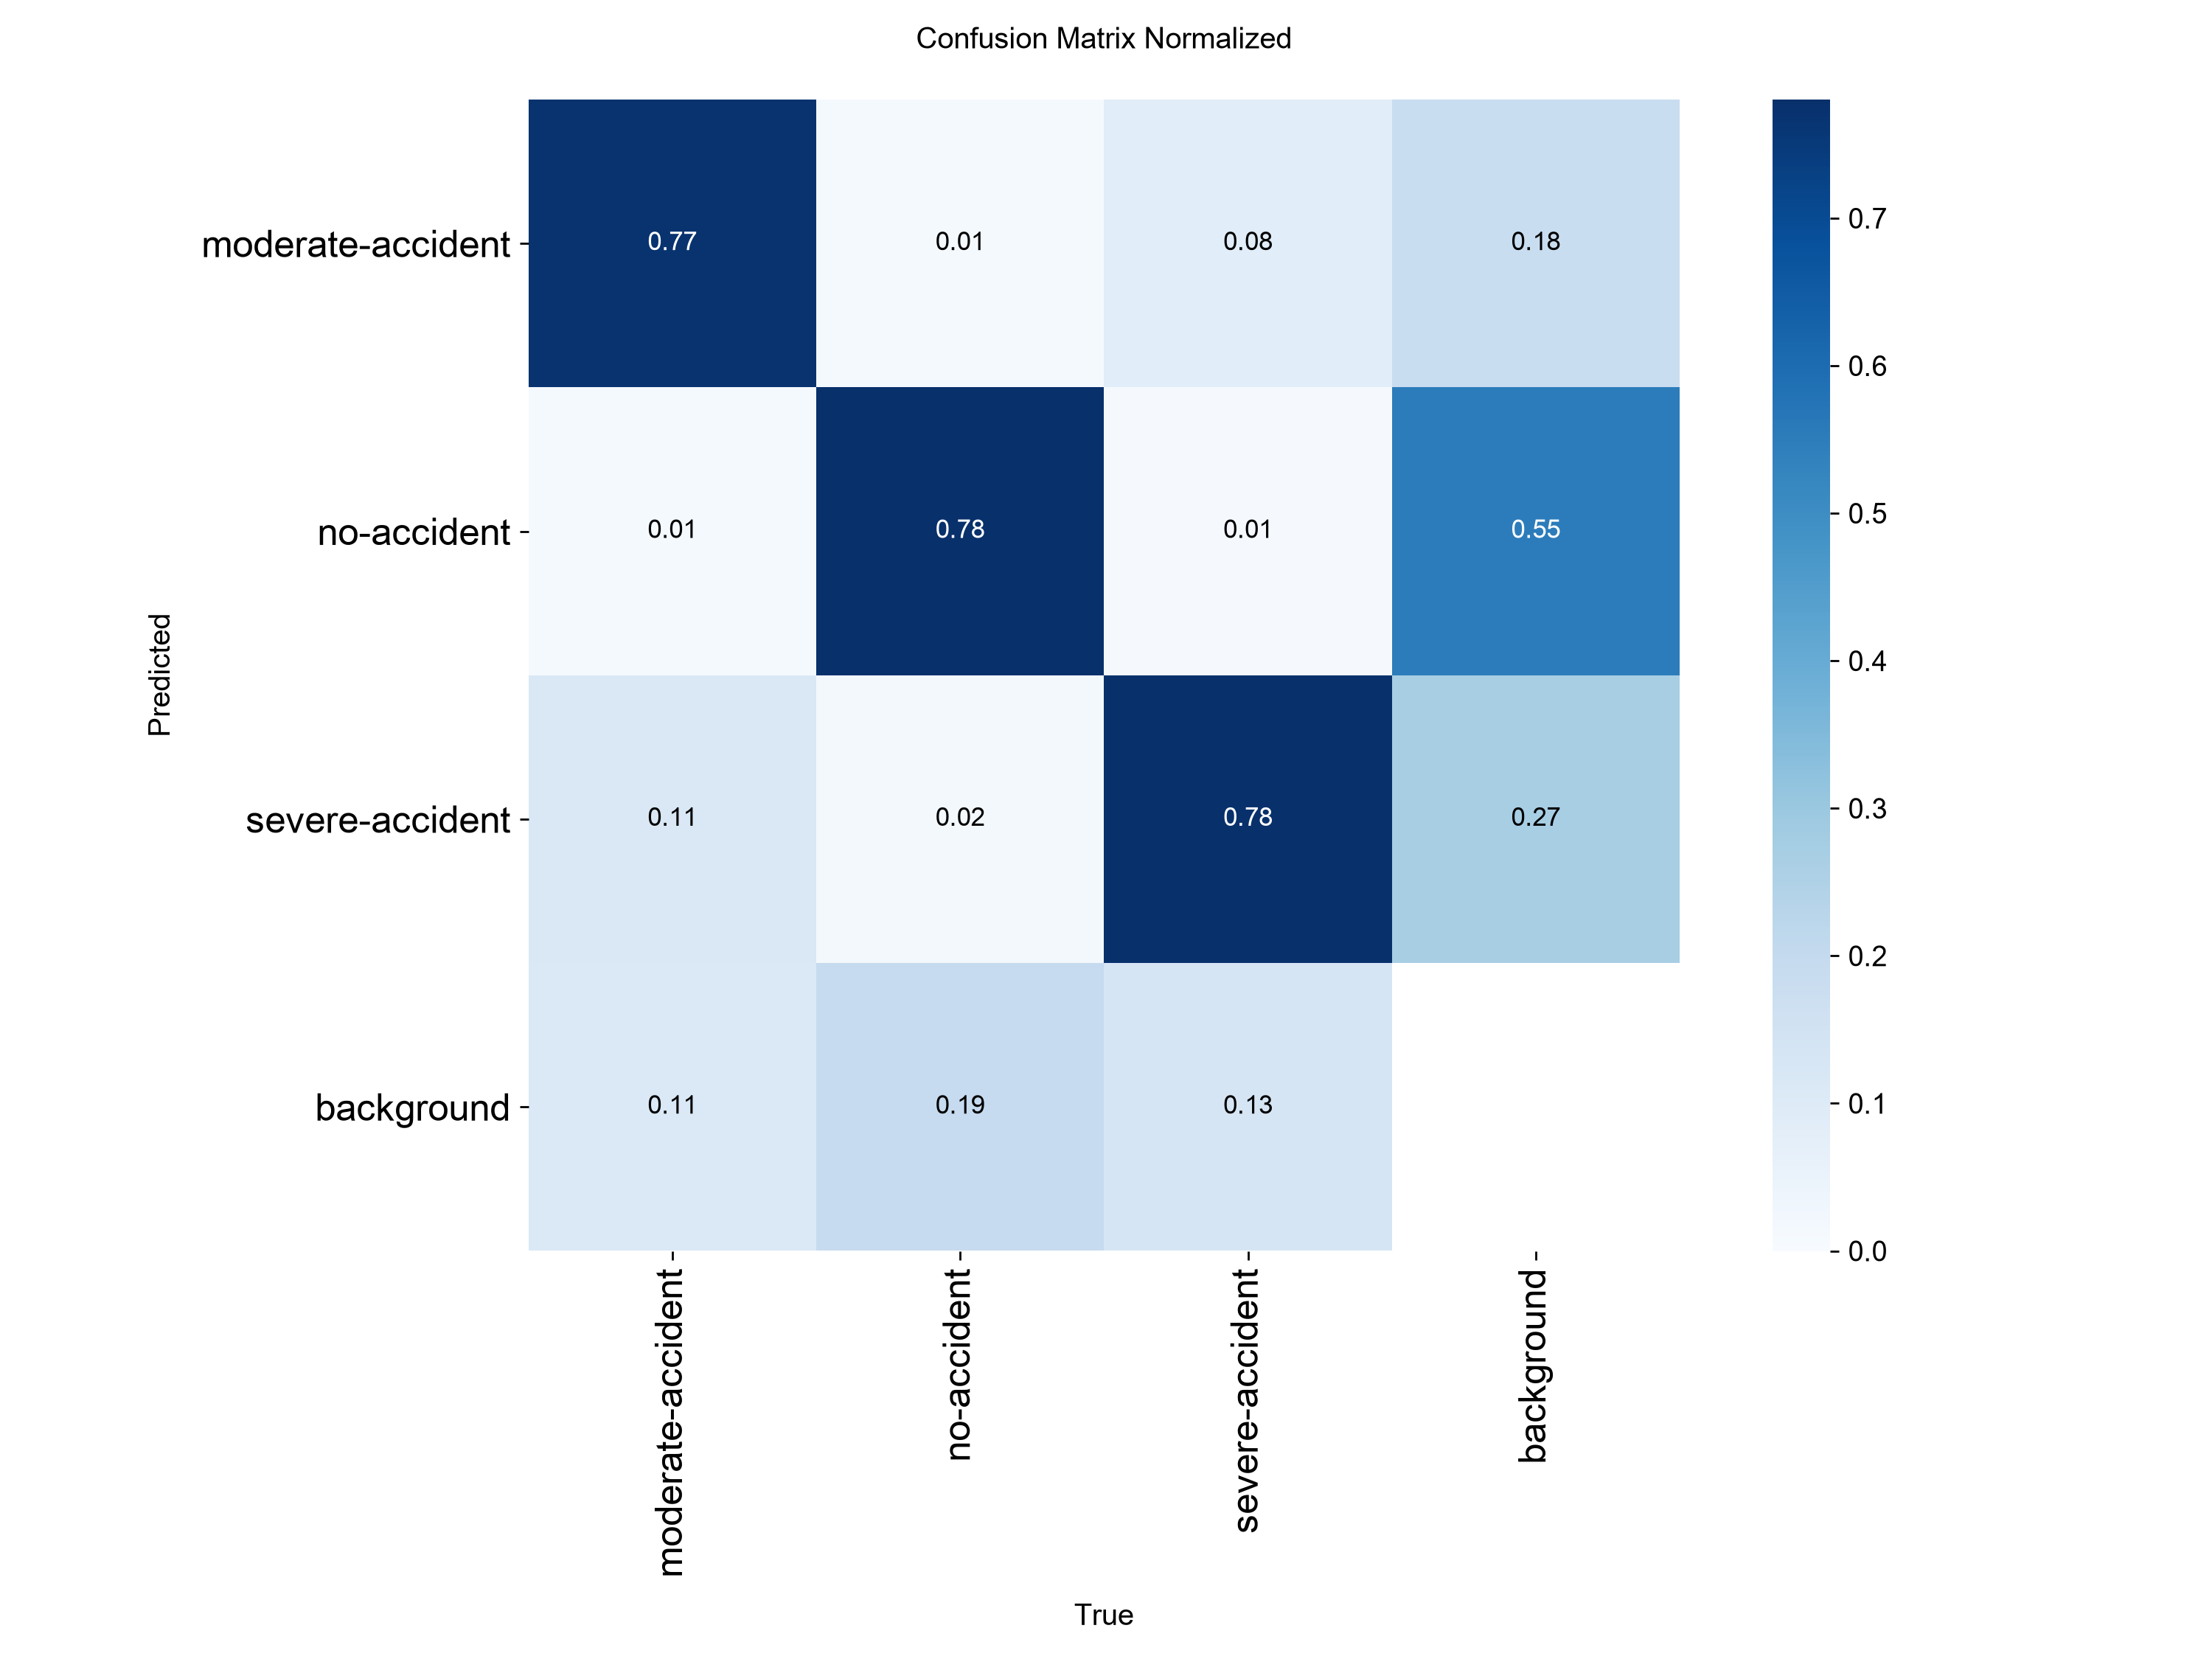
\includegraphics[width=\linewidth]{results/detection/accident_severity-2/confusion_matrix_normalized.png}\end{minipage}
\caption{Severity-run precision-recall curve and normalized validation confusion matrix.}
\label{fig:sev-curves}\end{figure}

\begin{figure}[t]\centering
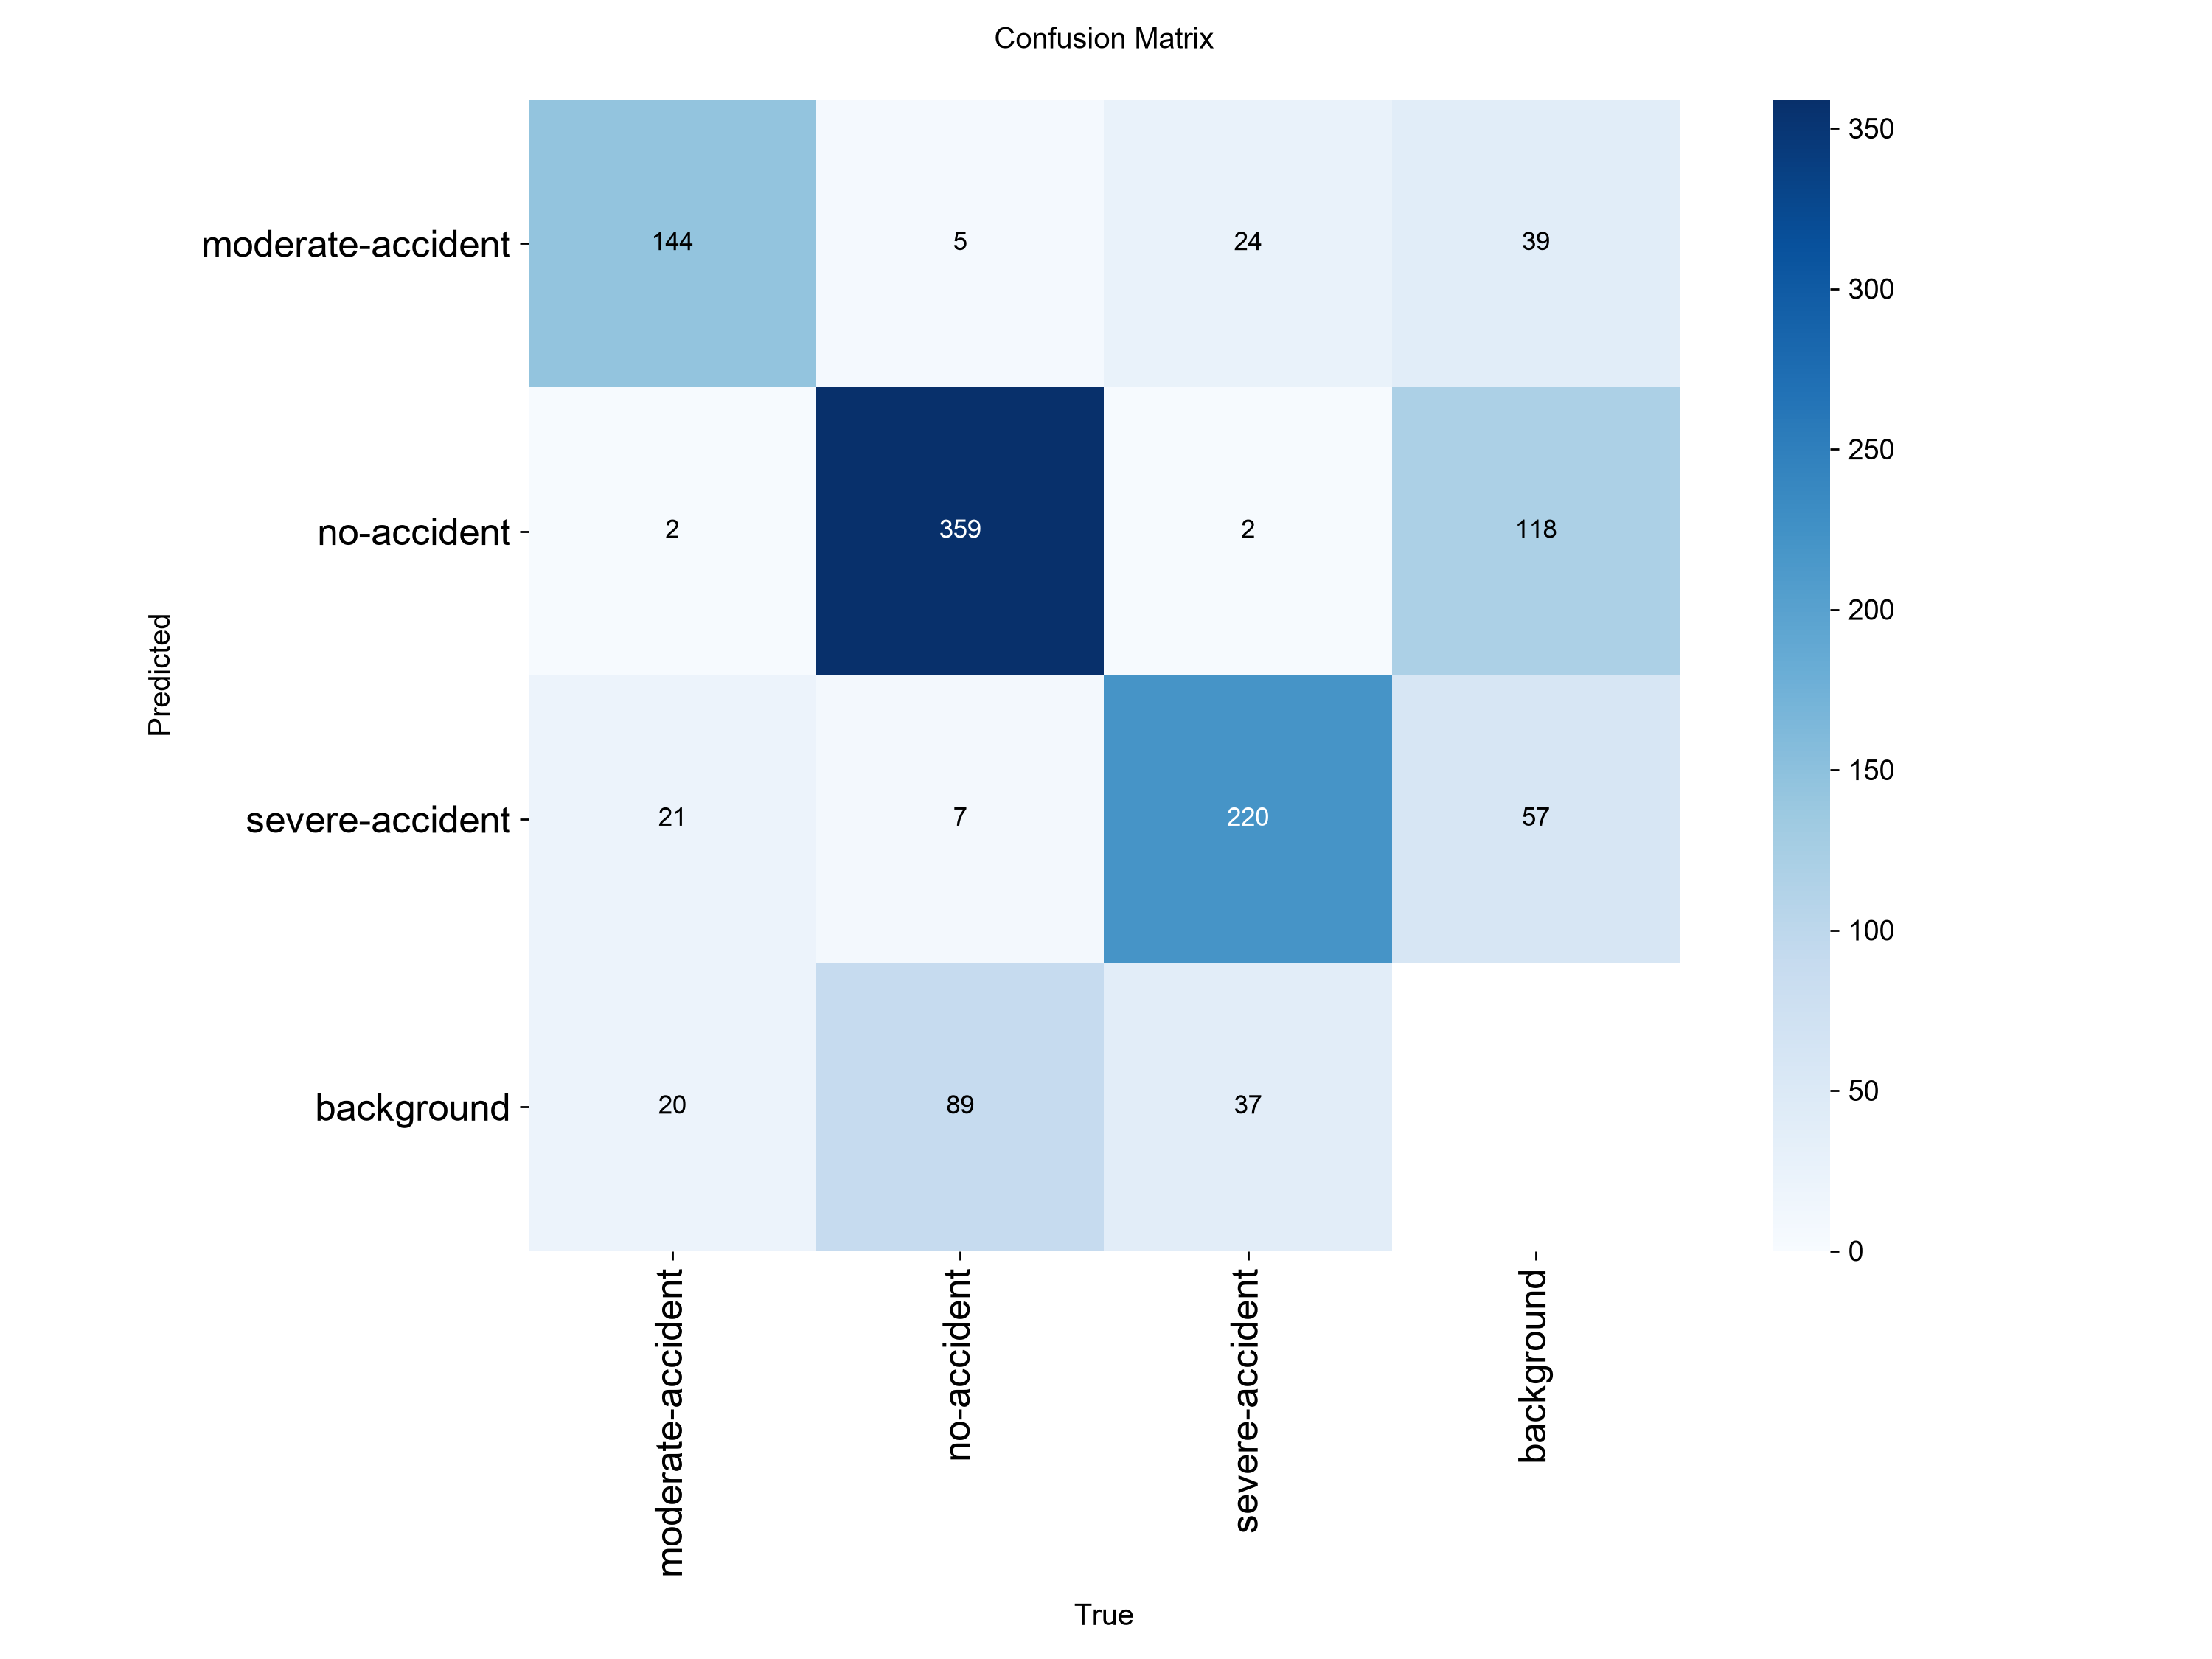
\includegraphics[width=0.86\textwidth]{results/detection/accident_severity-2/confusion_matrix.png}
\caption{Raw severity validation confusion matrix.}
\label{fig:sev-raw}\end{figure}
The severity test summary reports preprocessing 2.7 ms, inference 8.2 ms, and postprocessing 0.2 ms per image. Their 11.1-ms sum implies an idealized serial ceiling near 90 images/s before video decoding, model orchestration, overlays, and encoding. It is not an end-to-end benchmark.

The accident confidence curves expose the precision-recall trade-off as the score threshold changes. The aggregate F1 optimum is not necessarily the correct emergency-monitoring operating point: event prevalence, tolerance for missed incidents, duplicate alerts, and operator workload must determine threshold selection. A fixed threshold should be selected only after event-level replay on representative camera footage. The severity run's validation curves similarly describe box-level behavior, but a crop-level or incident-level severity decision needs a separate aggregation and calibration evaluation.

\begin{figure}[t]\centering
\begin{minipage}{0.48\textwidth}\centering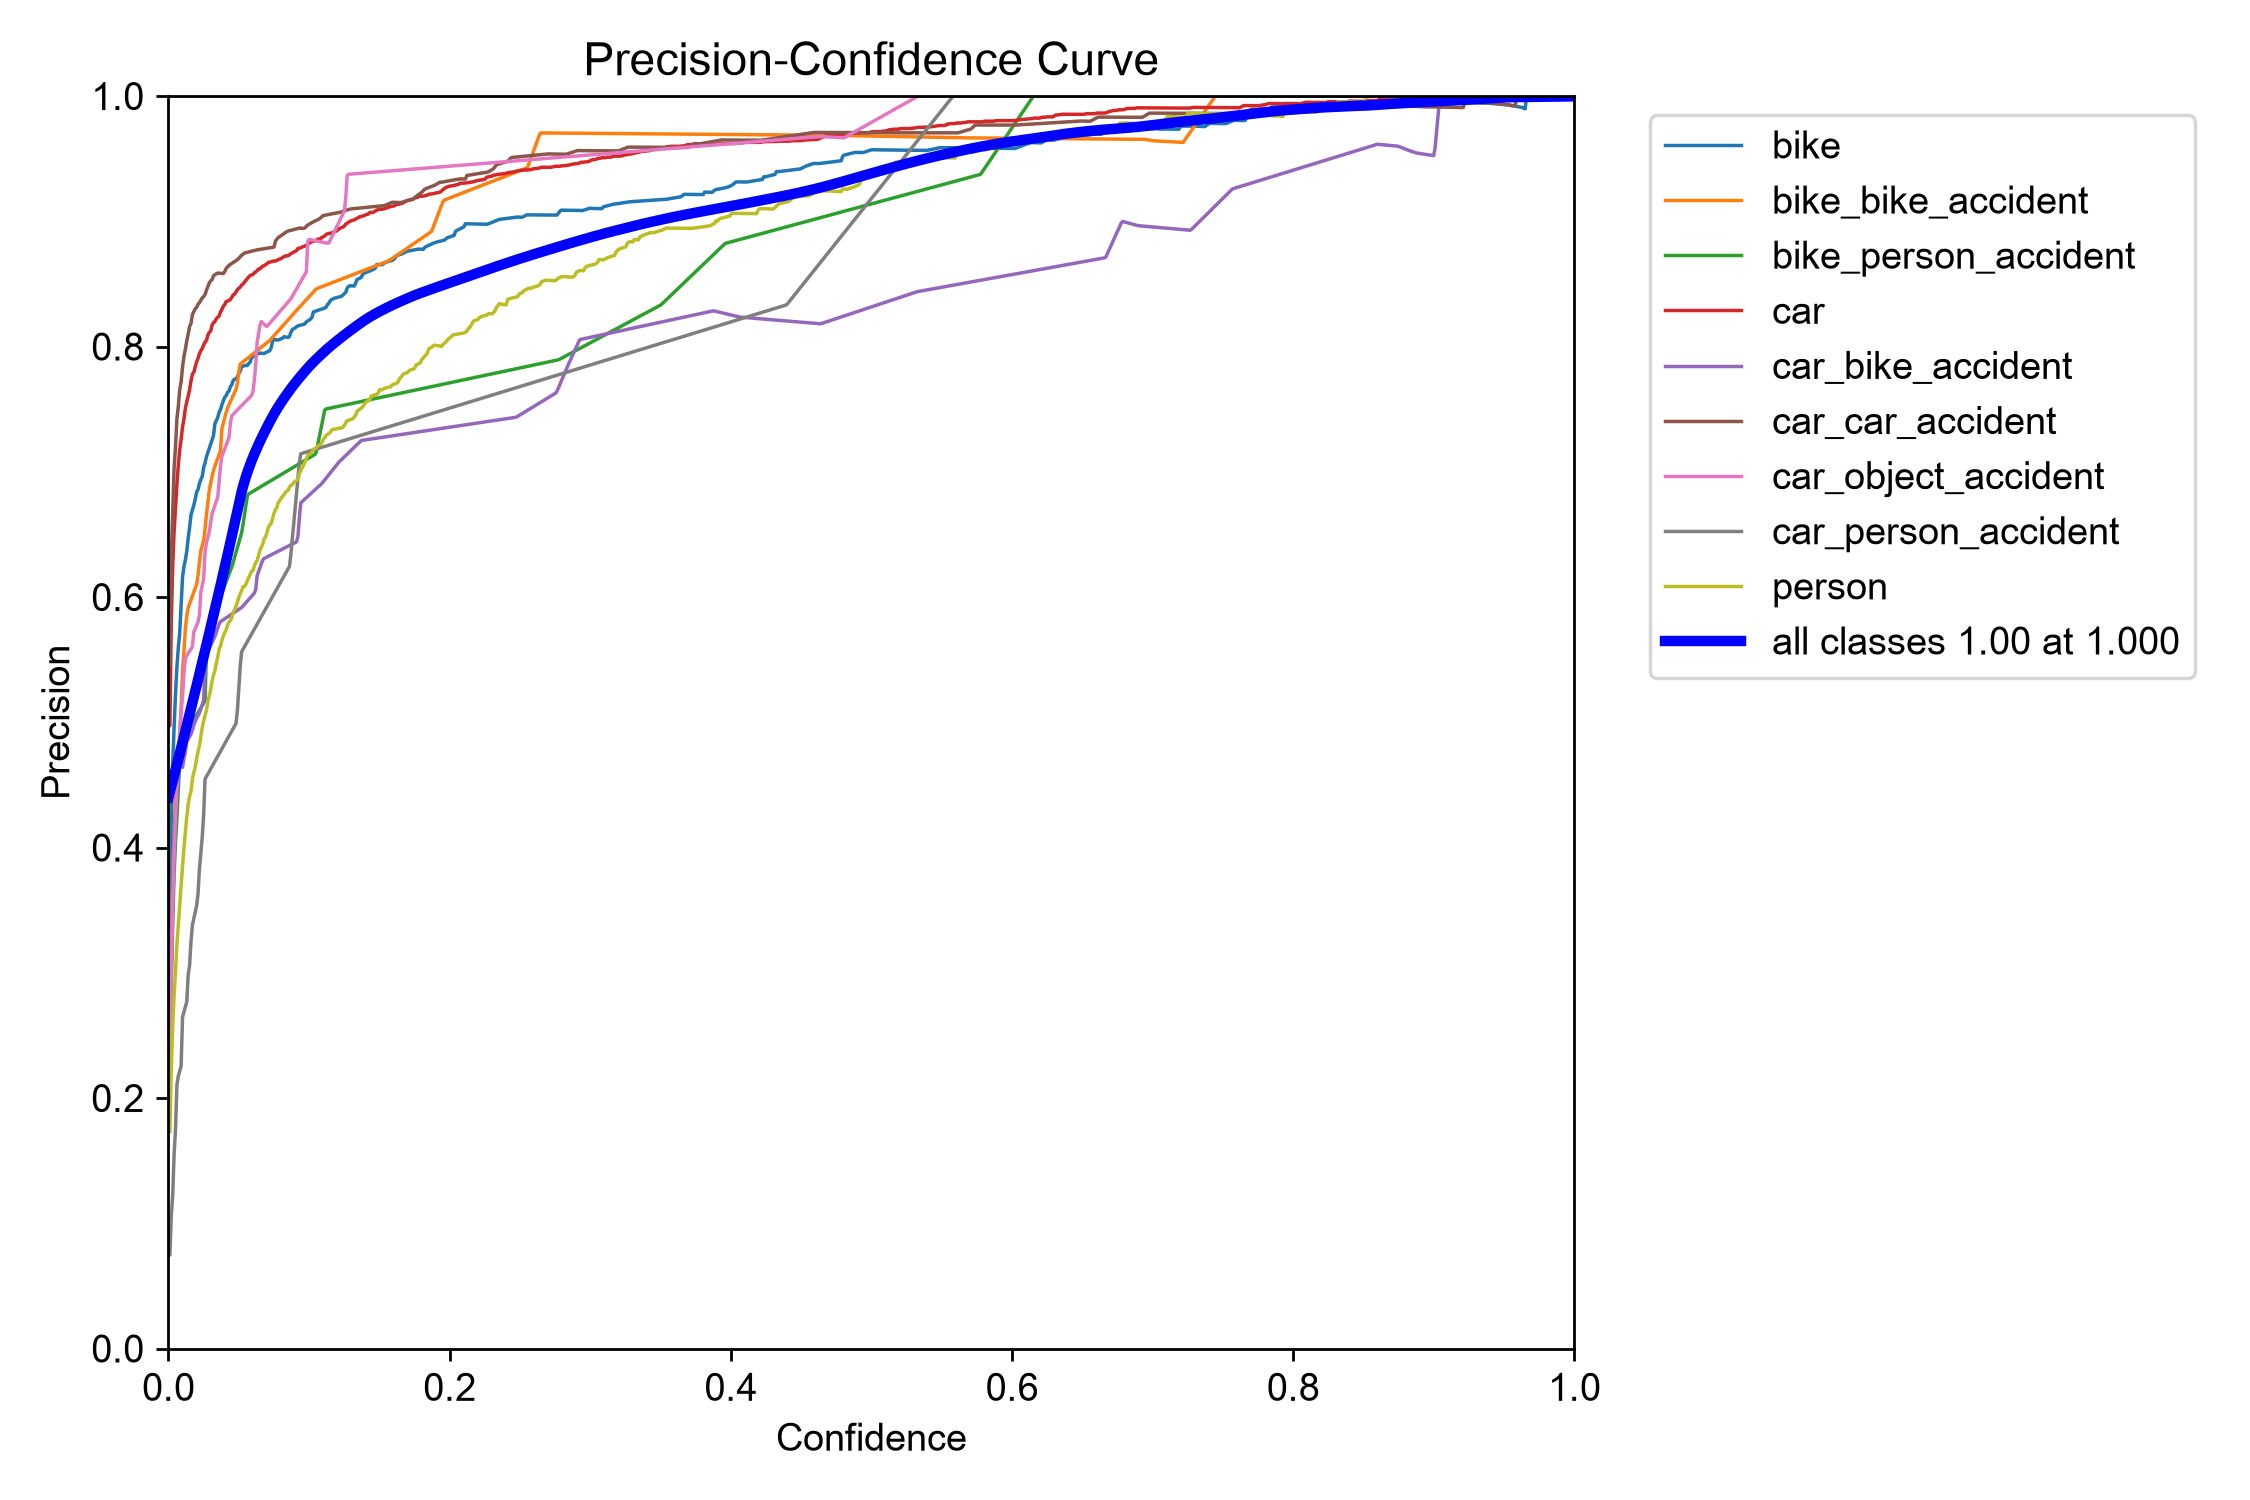
\includegraphics[width=\linewidth]{results/detection/yolo26_baseline/BoxP_curve.png}\end{minipage}\hfill
\begin{minipage}{0.48\textwidth}\centering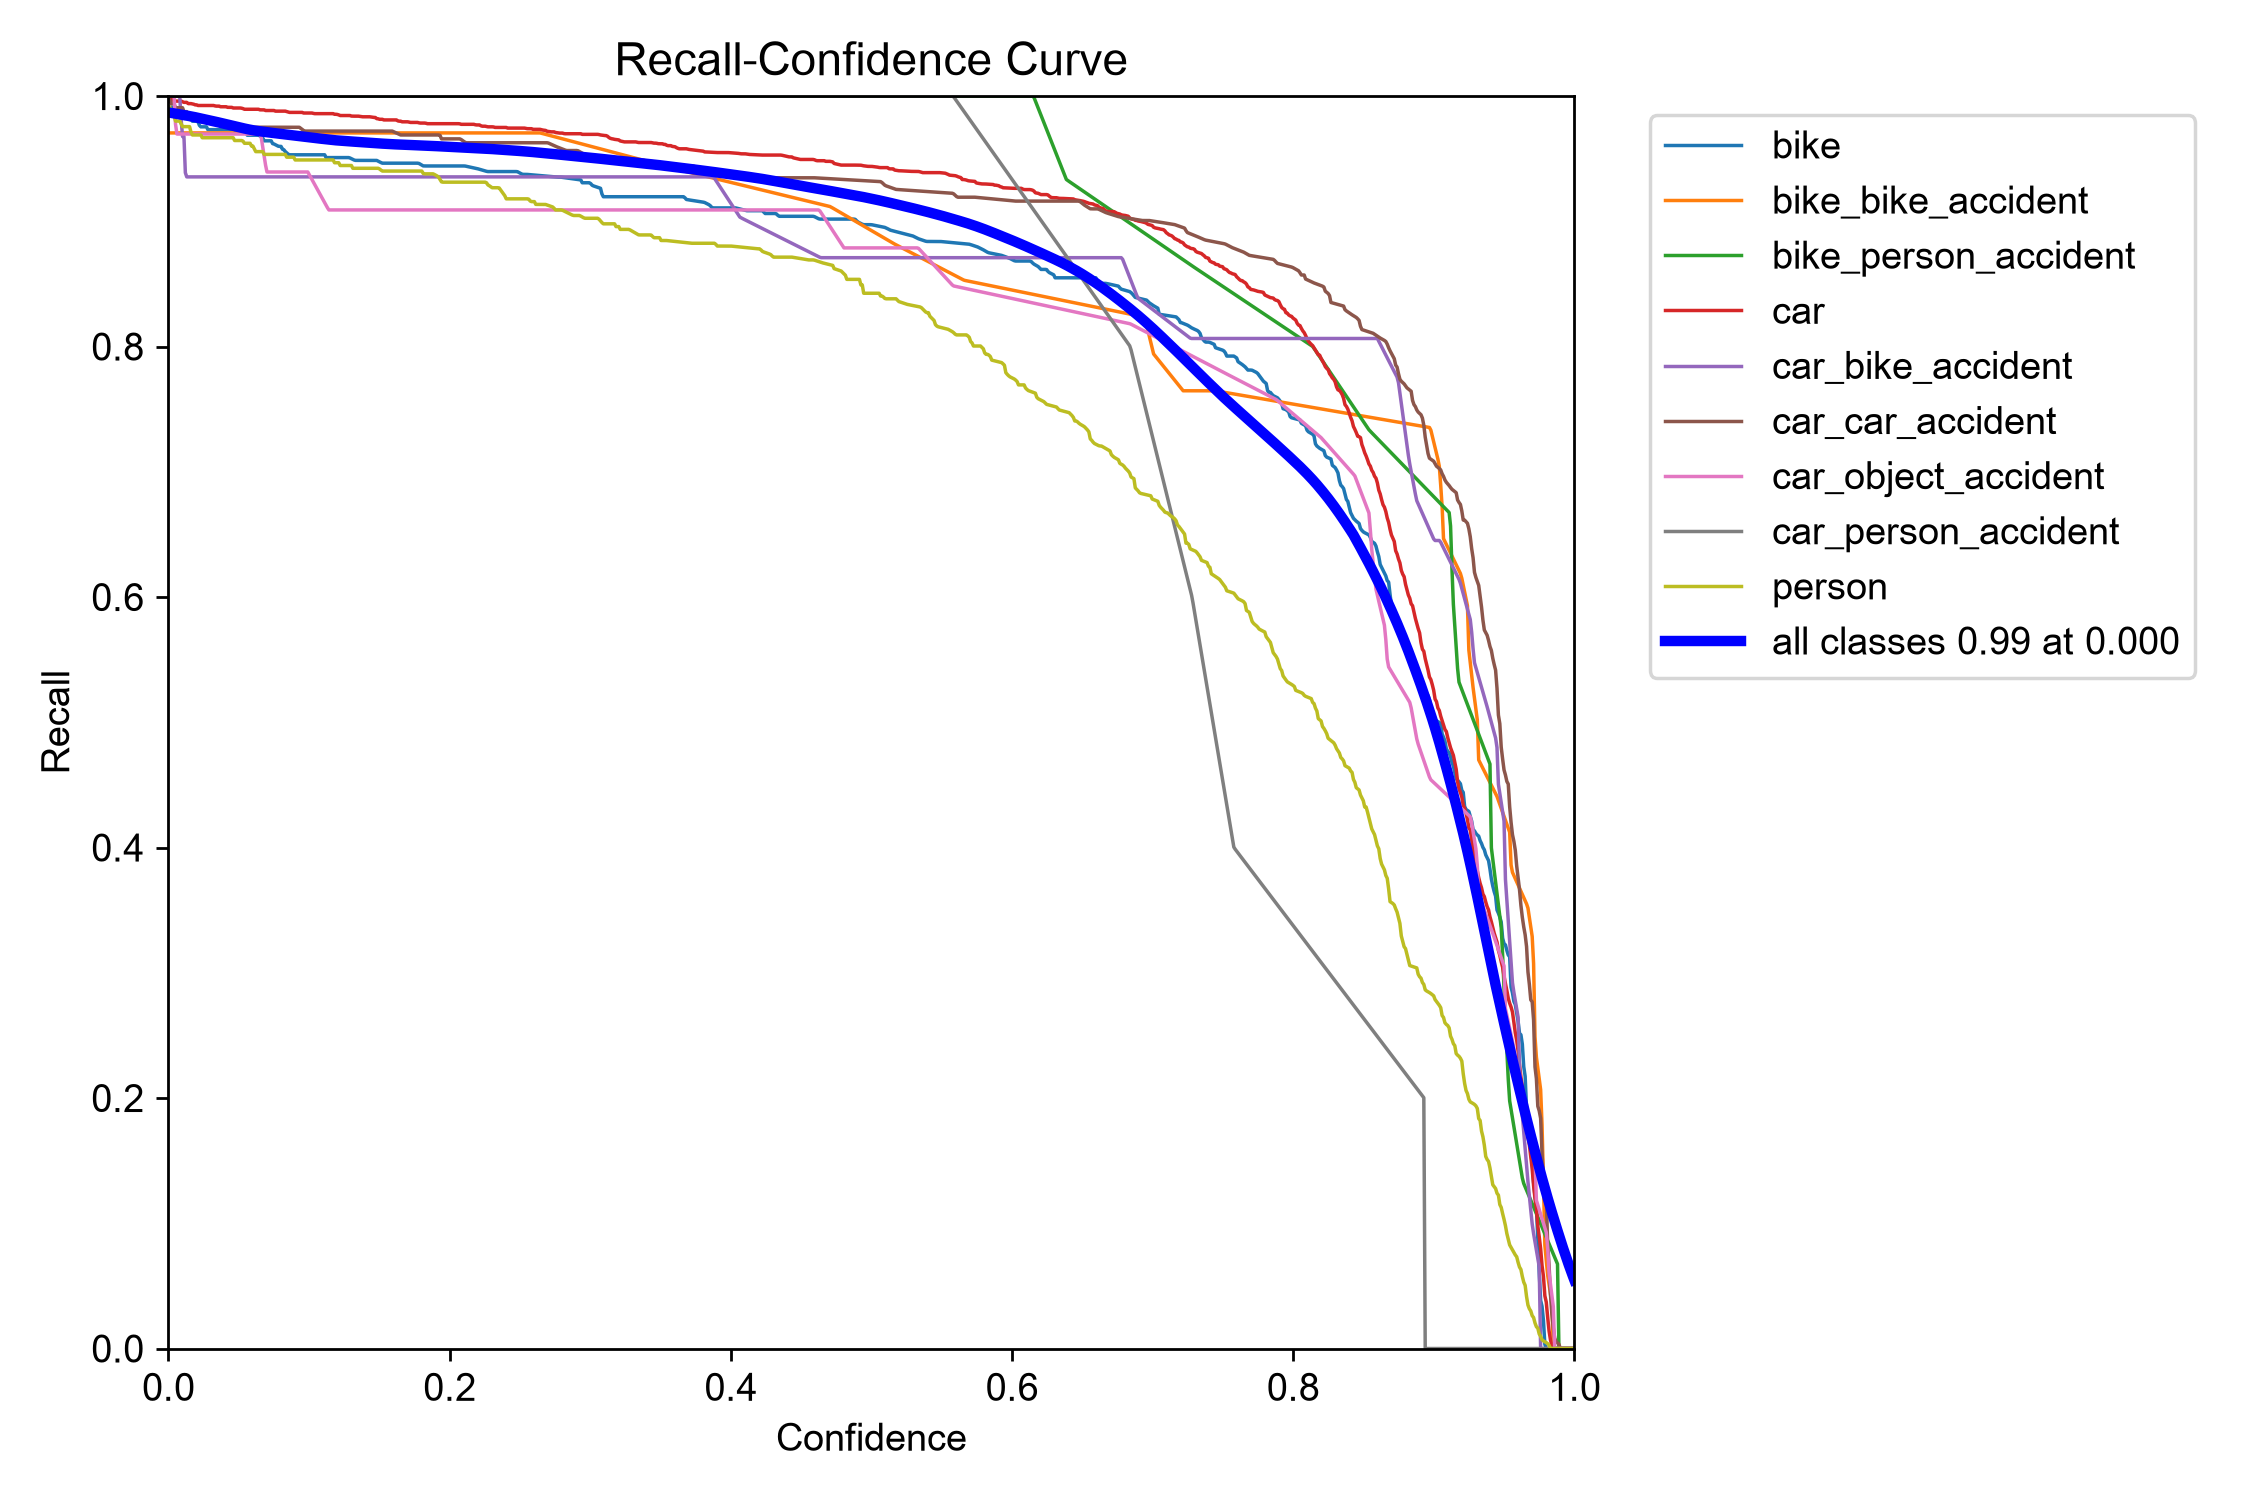
\includegraphics[width=\linewidth]{results/detection/yolo26_baseline/BoxR_curve.png}\end{minipage}
\caption{Accident detector precision and recall as confidence threshold changes.}
\label{fig:acc-pr-threshold}\end{figure}
\begin{figure}[t]\centering
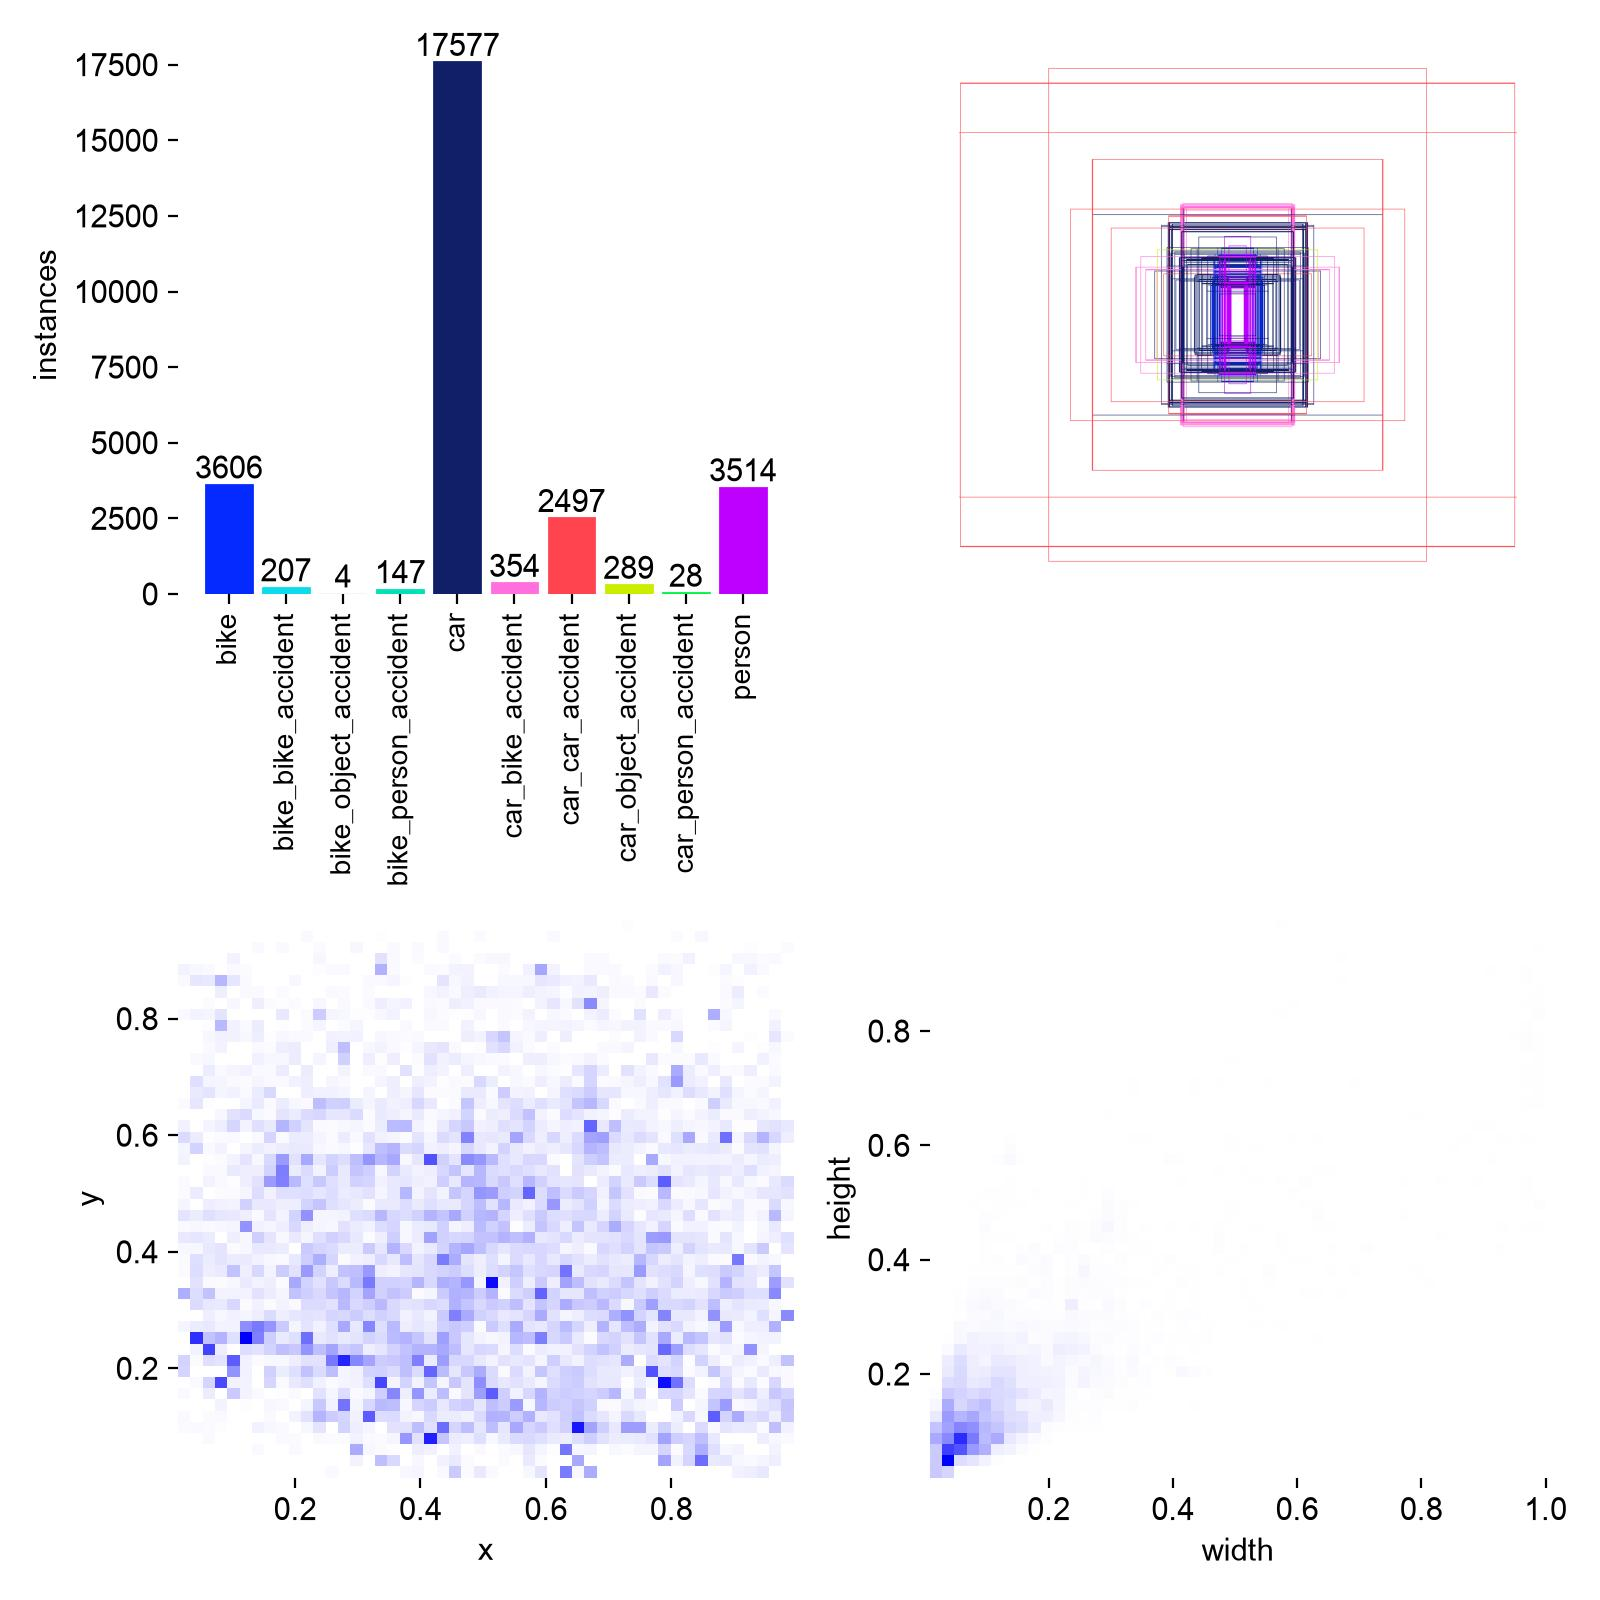
\includegraphics[width=0.72\textwidth]{results/detection/yolo26_baseline/labels.jpg}
\caption{Accident training-label counts and normalized box geometry. The rare interaction classes are difficult to inspect at this scale; Table~\ref{tab:classes} gives the count values.}
\label{fig:acc-labels}\end{figure}
\begin{figure}[t]\centering
\begin{minipage}{0.48\textwidth}\centering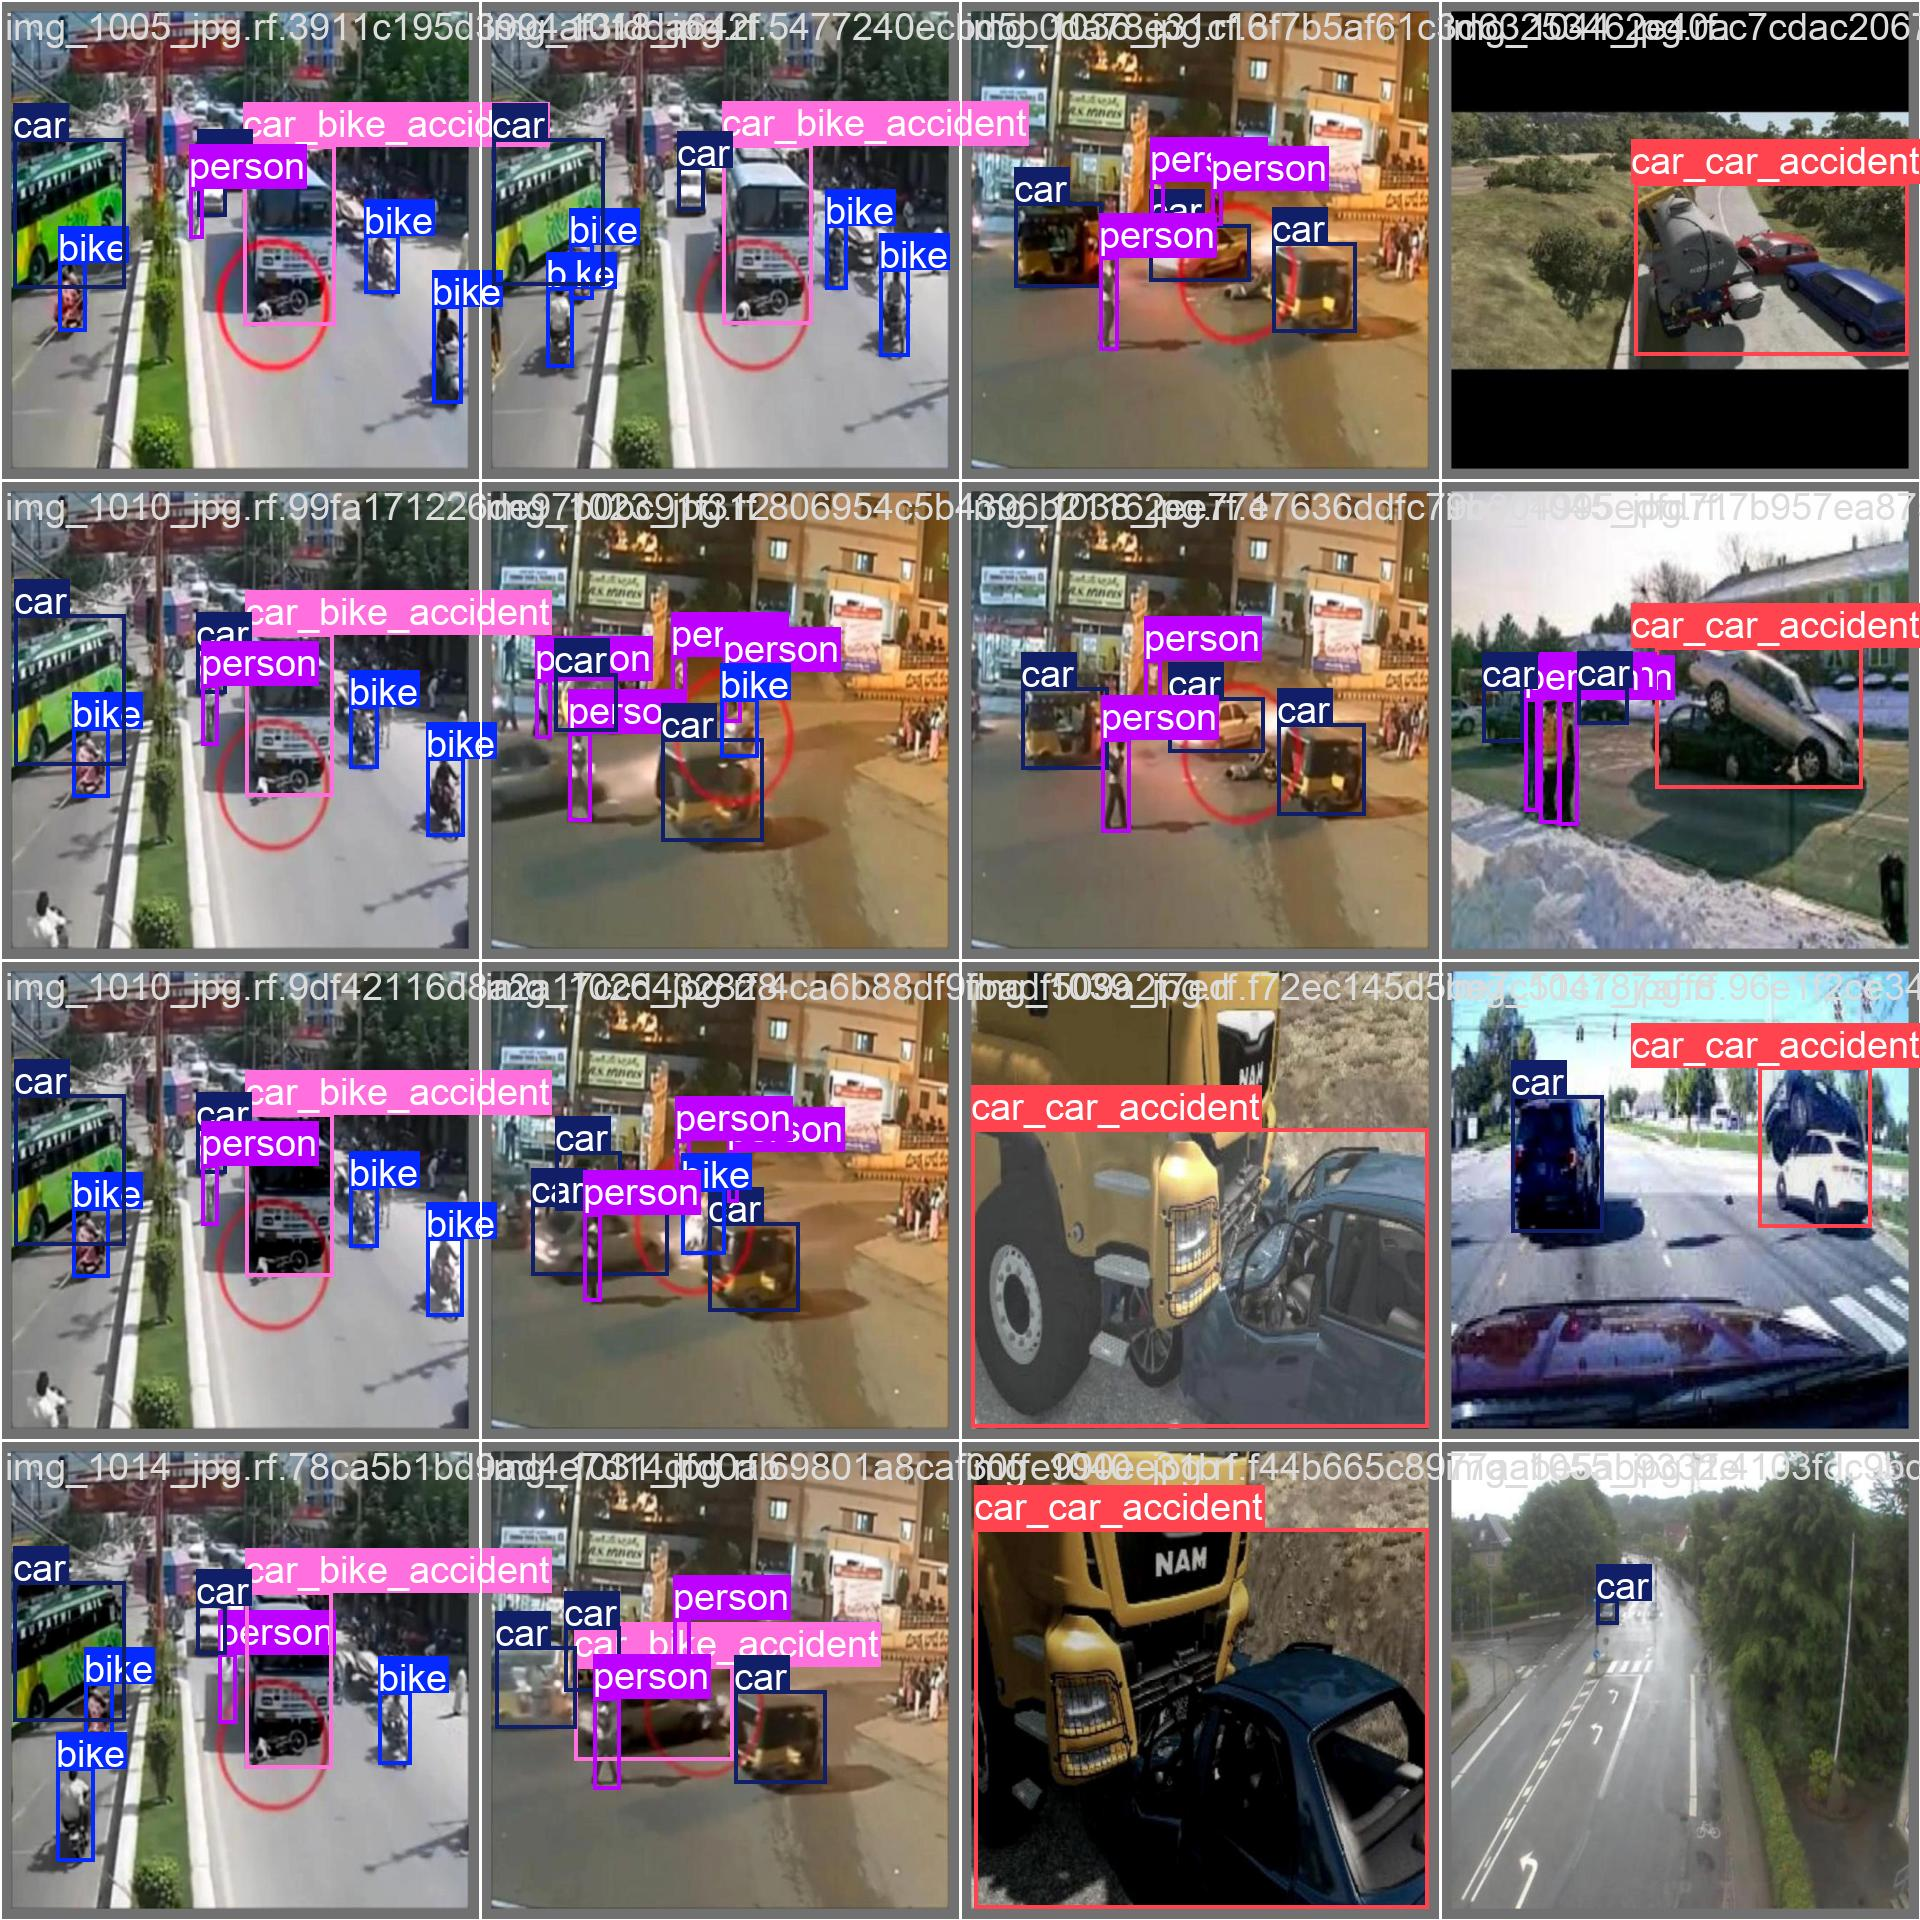
\includegraphics[width=\linewidth]{results/detection/yolo26_baseline/val_batch0_labels.jpg}\end{minipage}\hfill
\begin{minipage}{0.48\textwidth}\centering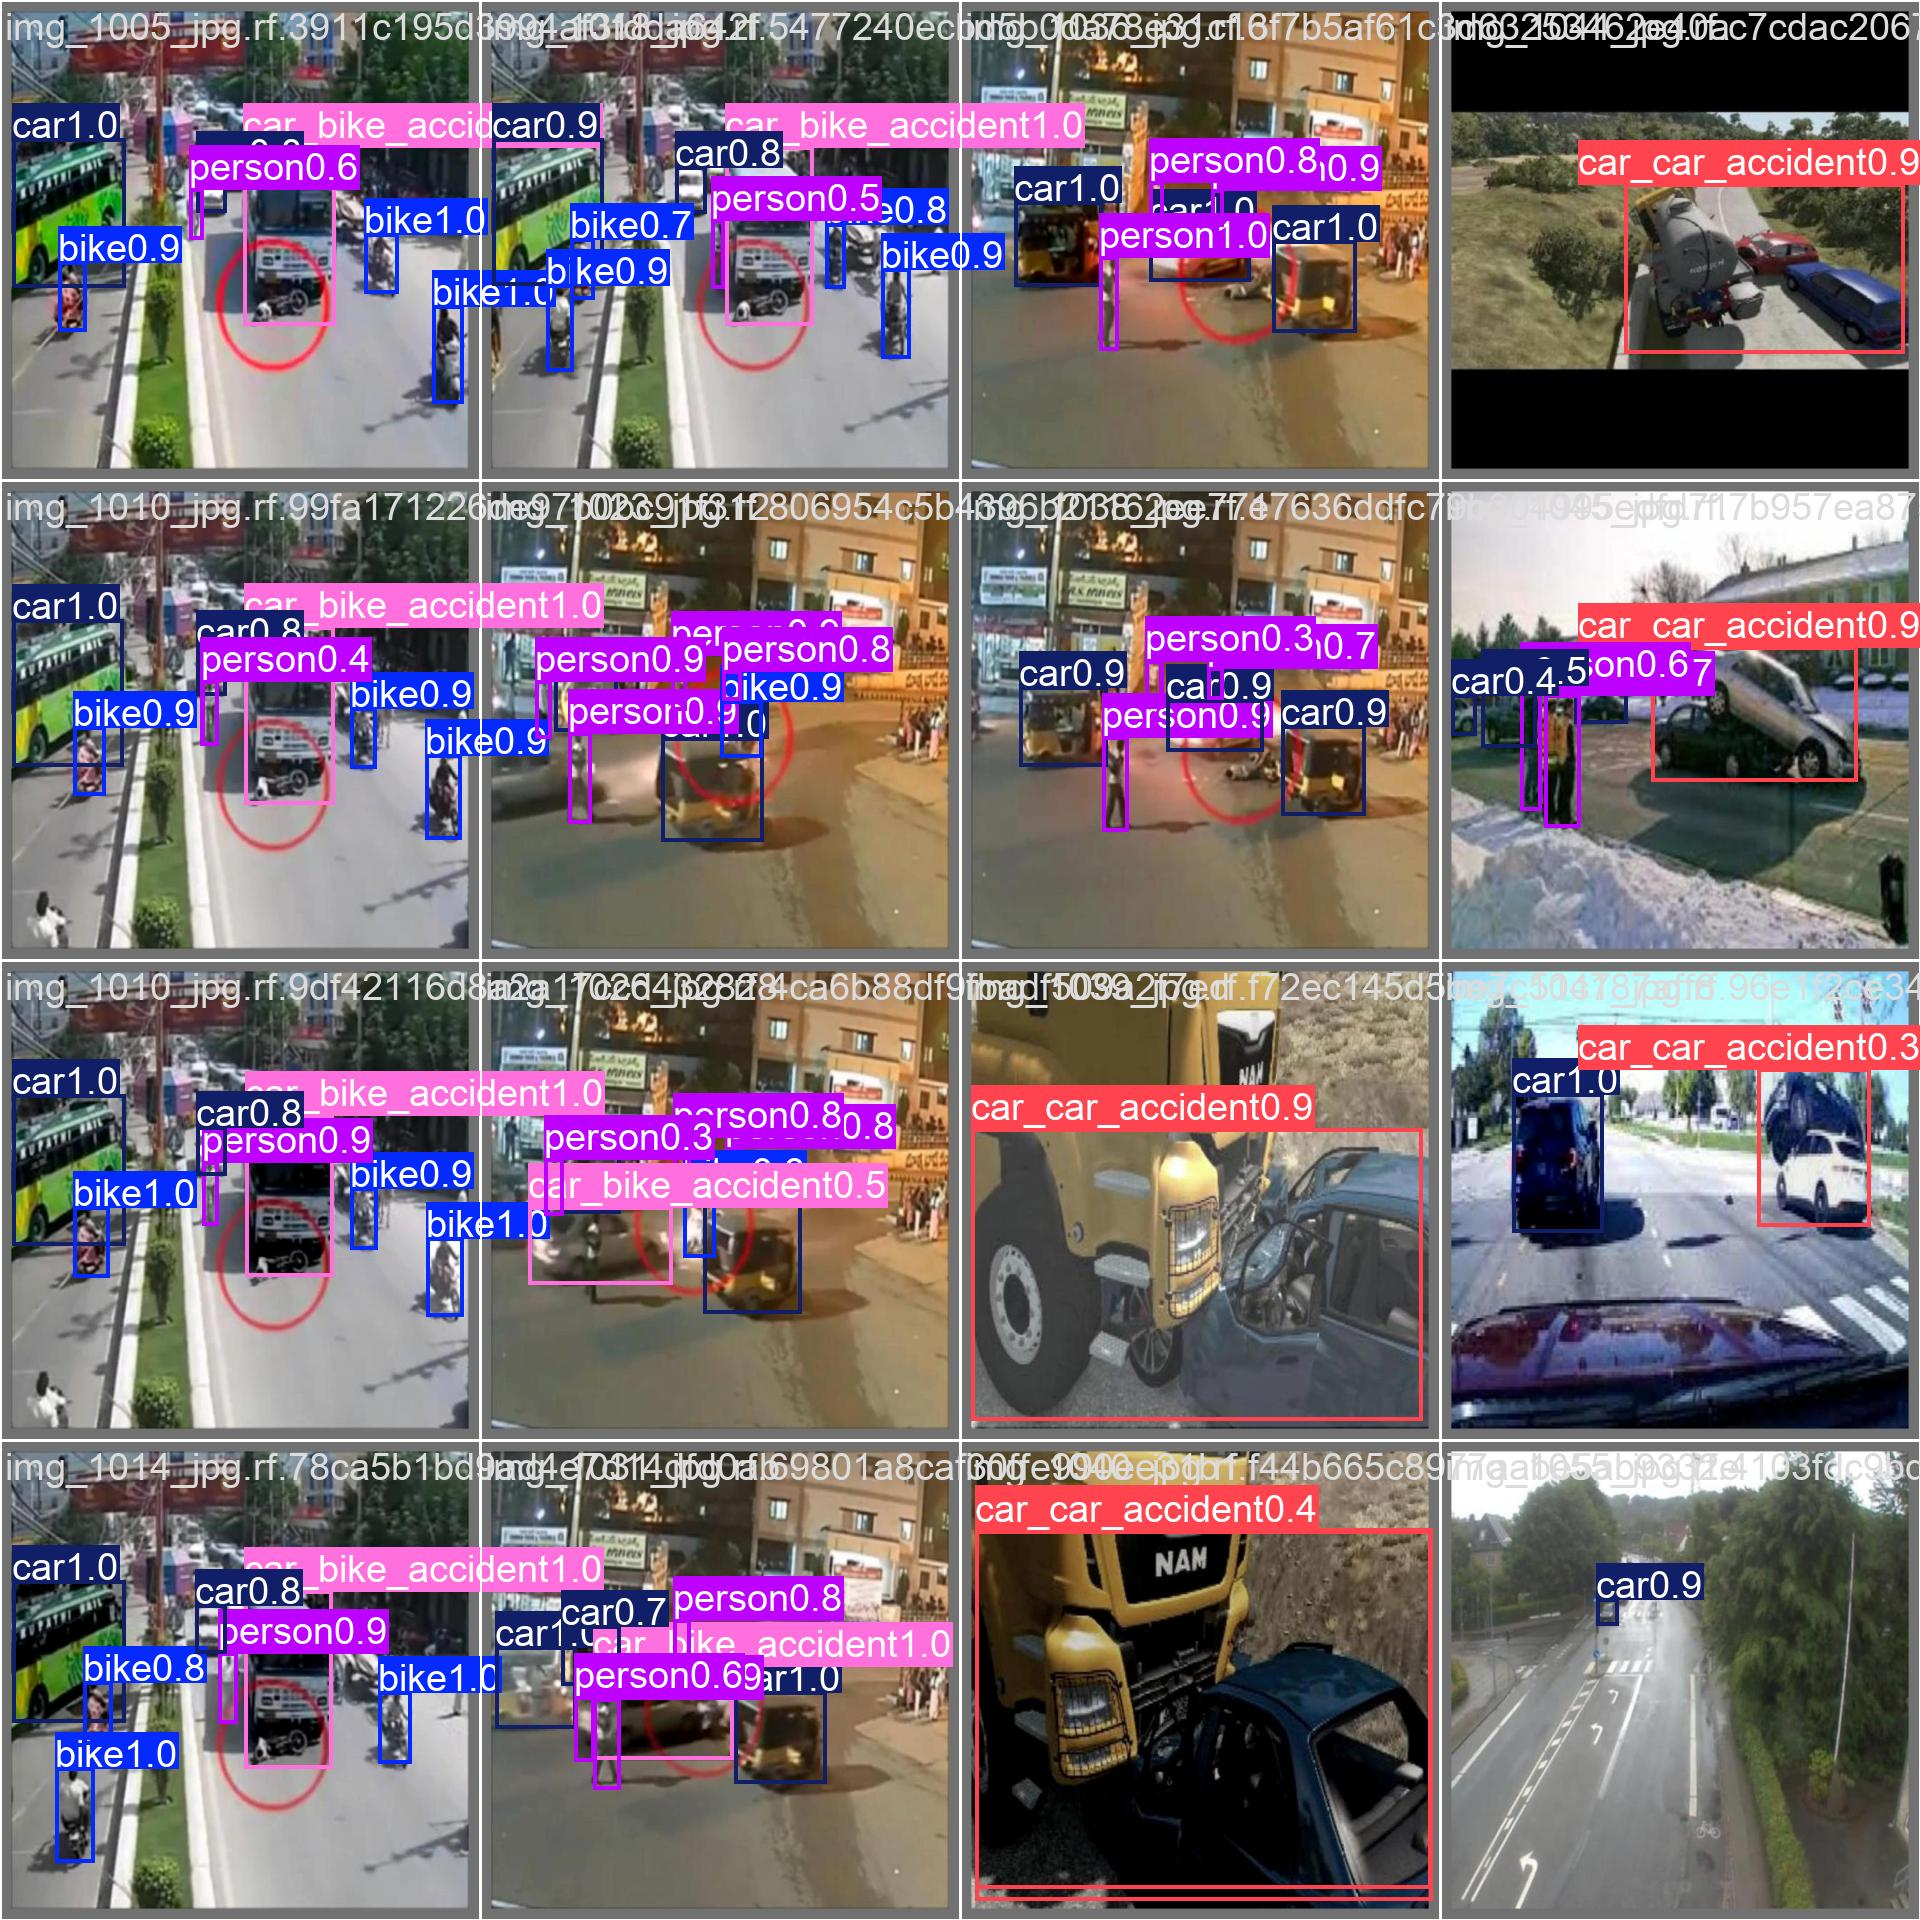
\includegraphics[width=\linewidth]{results/detection/yolo26_baseline/val_batch0_pred.jpg}\end{minipage}
\caption{Representative accident validation batch: ground-truth labels and model predictions.}
\label{fig:acc-example}\end{figure}

Severity validation performance is lower than accident detection on the saved aggregate metrics. The separate test result confirms a modest decline from the best validation summary, but the absent uncertainty interval prevents claims about the size or statistical significance of a generalization gap. The moderate, no-accident, and severe categories have an ordered meaning, yet ordinary mAP does not penalize a low-to-high confusion more than an adjacent-class confusion. Class-wise recall, macro-F1, balanced accuracy, ordinal error, and calibration should accompany future severity results. The saved model's per-class test AP values are close, while recall is lower than precision for no-accident and severe labels. That pattern merits threshold and confusion analysis, not a medical interpretation.

\begin{figure}[t]\centering
\begin{minipage}{0.48\textwidth}\centering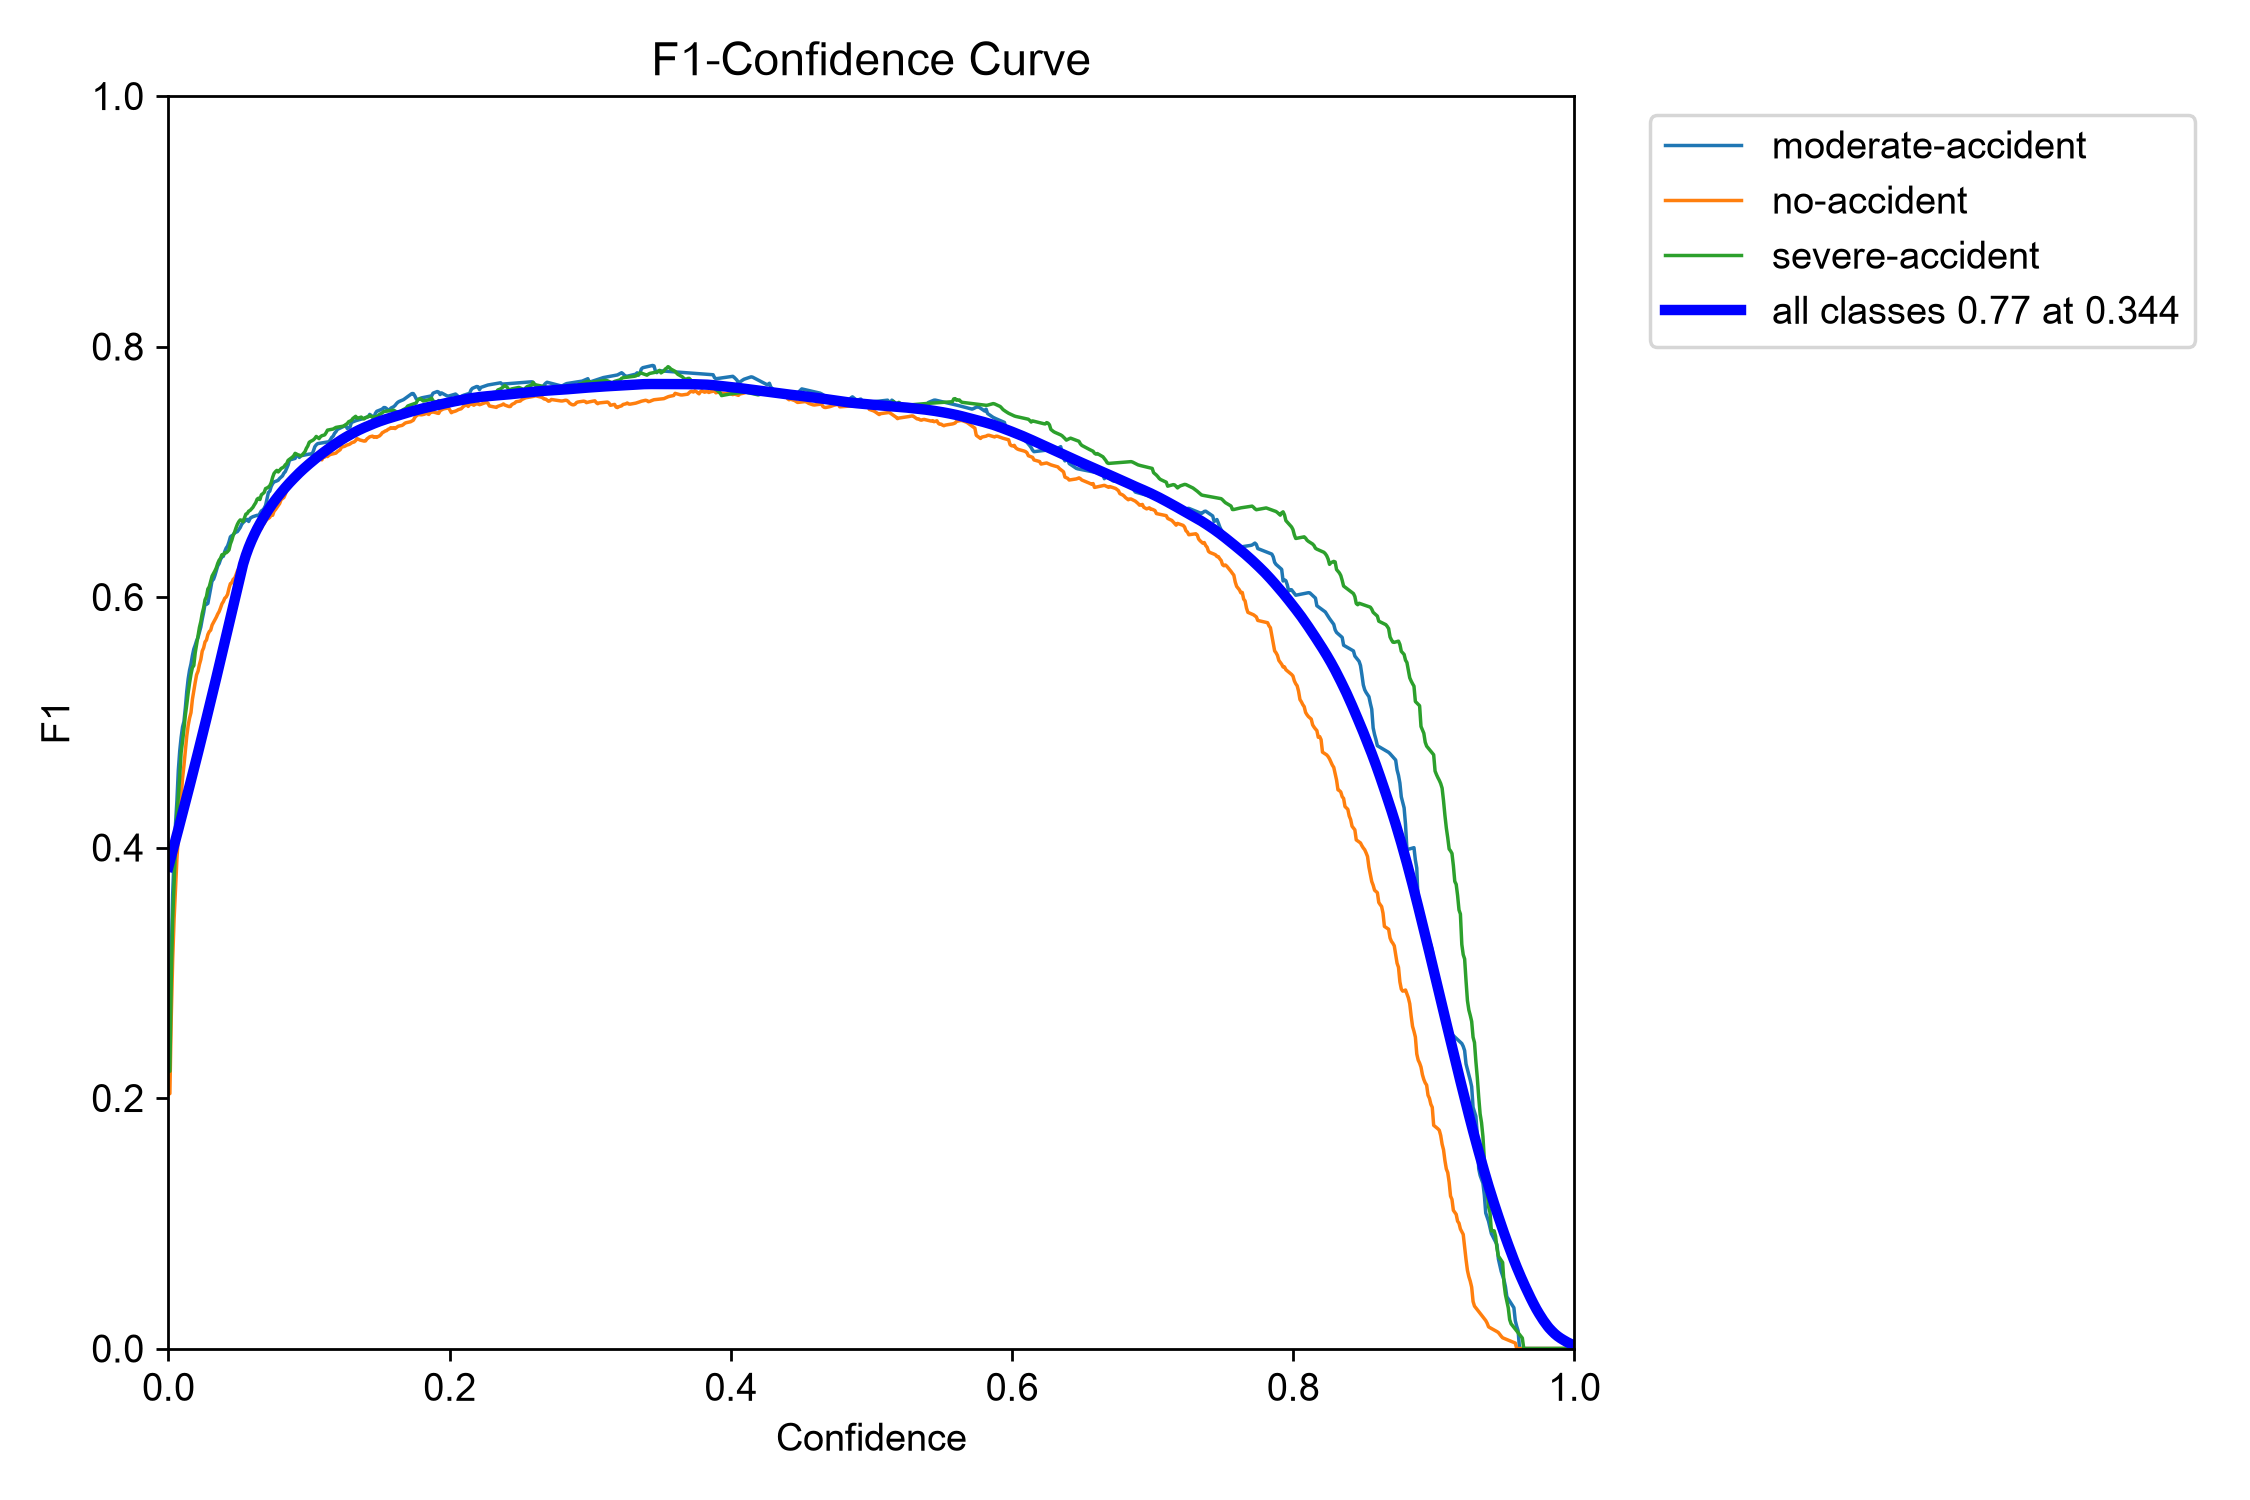
\includegraphics[width=\linewidth]{results/detection/accident_severity-2/BoxF1_curve.png}\end{minipage}\hfill
\begin{minipage}{0.48\textwidth}\centering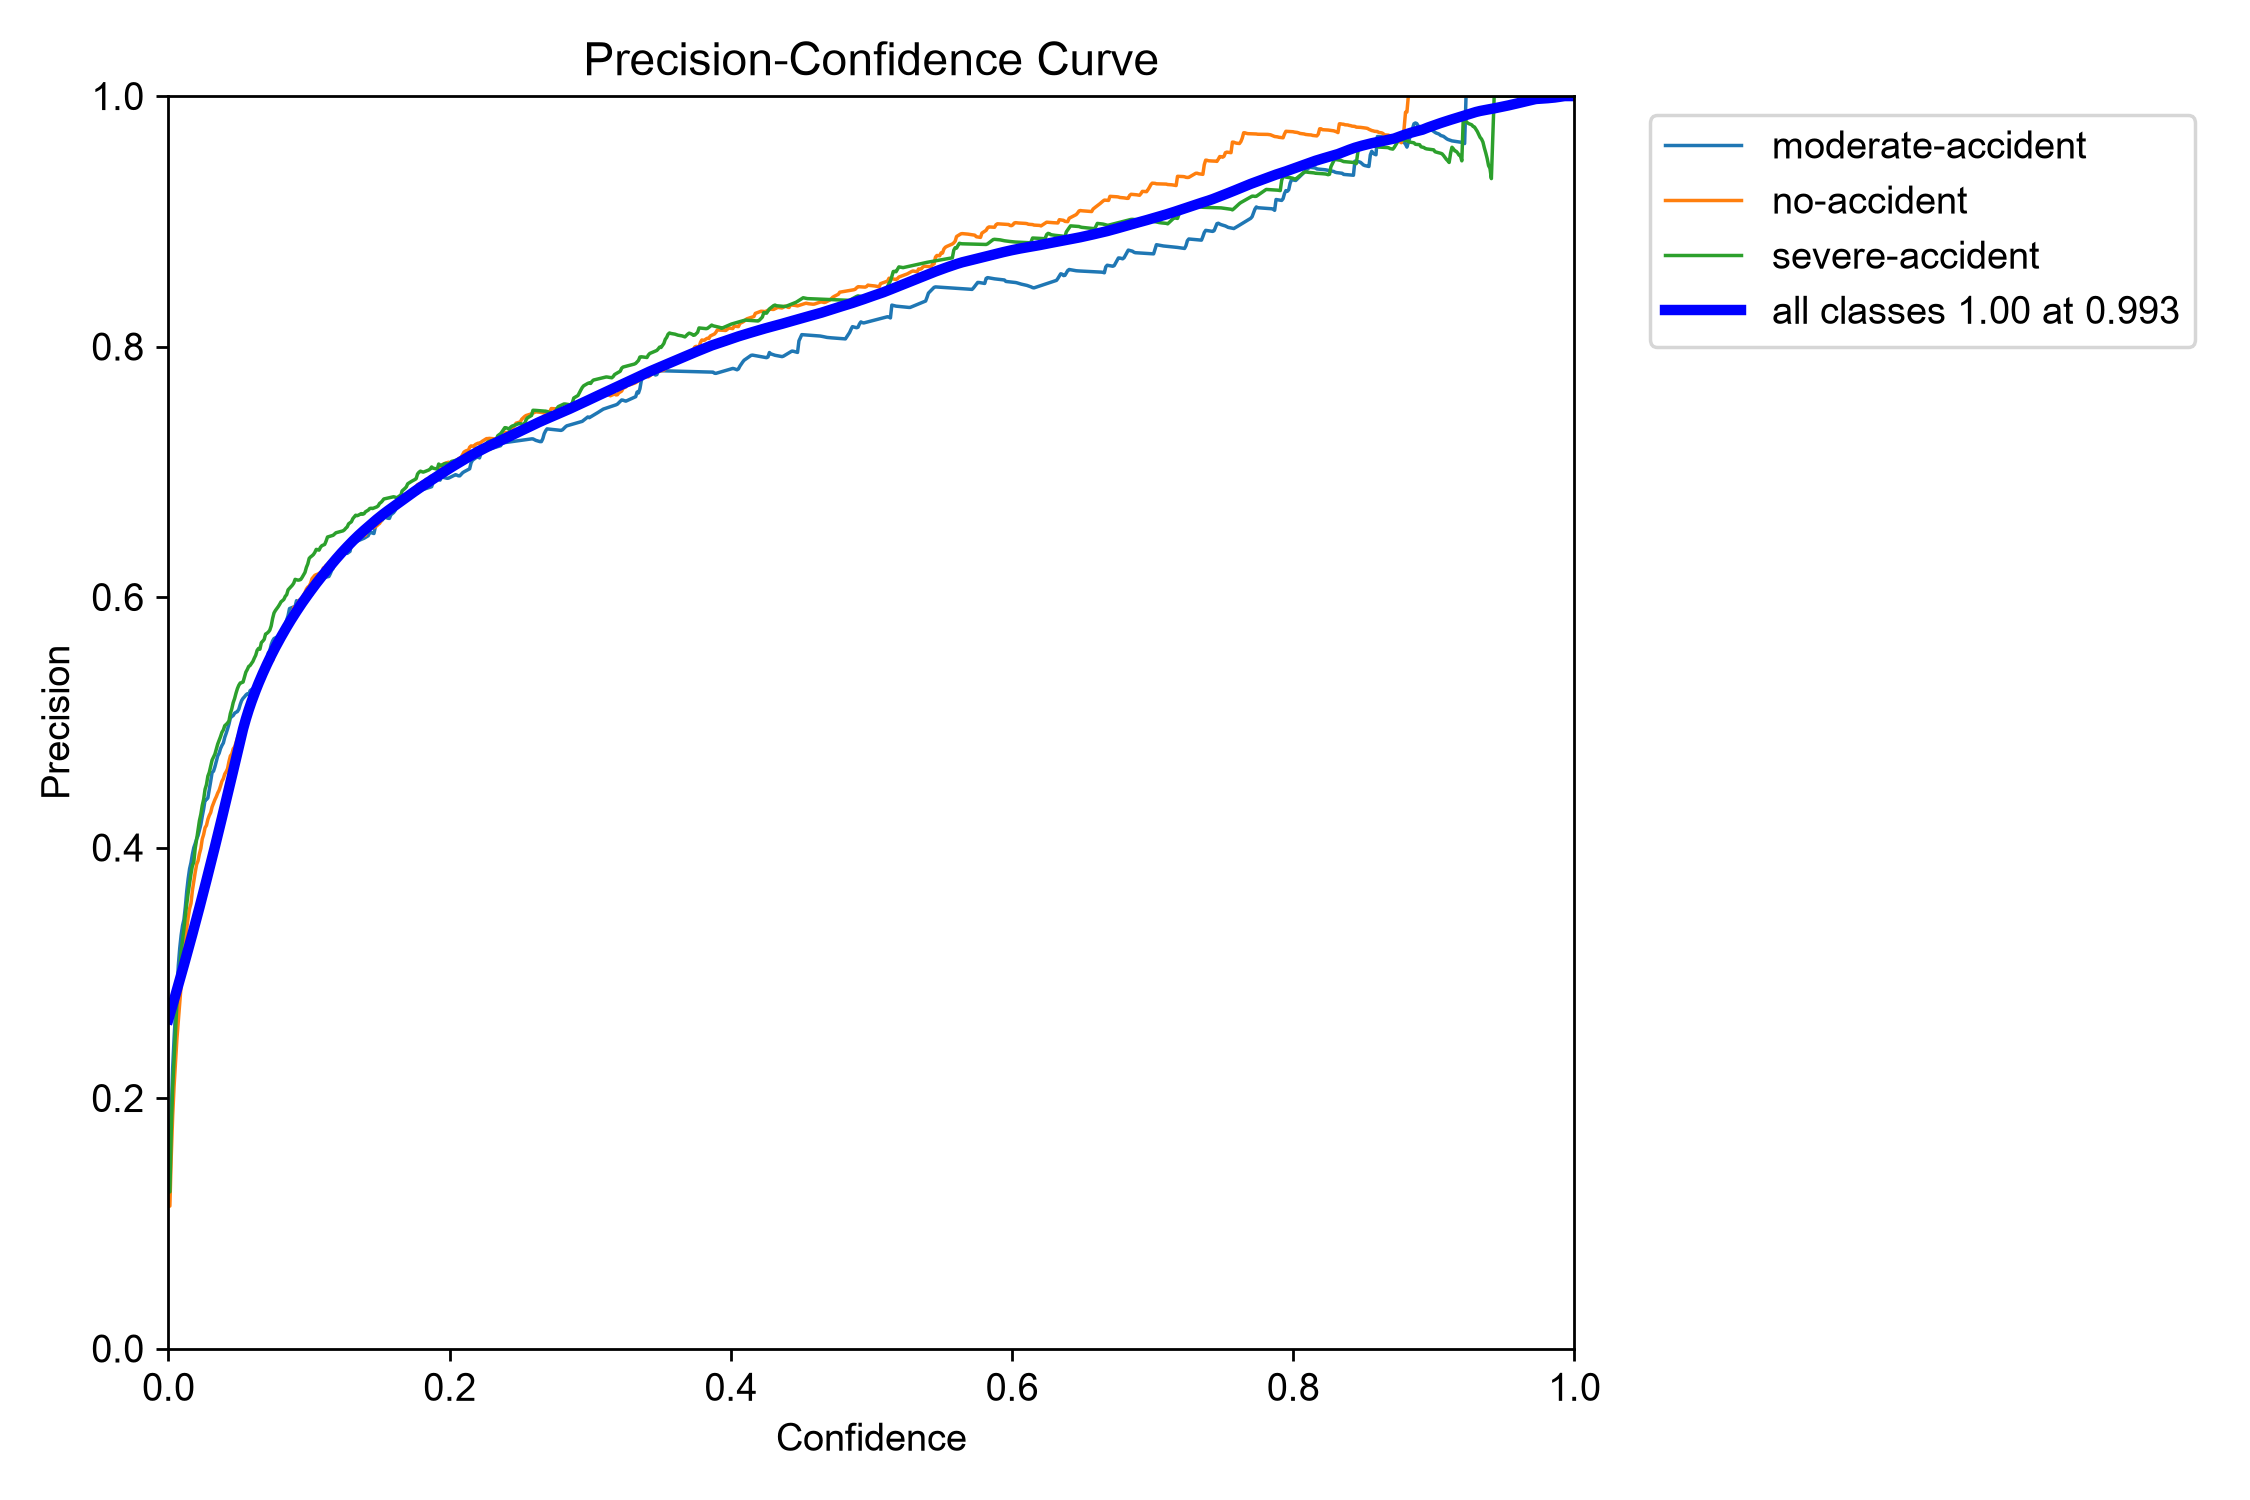
\includegraphics[width=\linewidth]{results/detection/accident_severity-2/BoxP_curve.png}\end{minipage}
\caption{Severity-run confidence-dependent F1 and precision curves.}
\label{fig:sev-threshold}\end{figure}
\begin{figure}[t]\centering
\begin{minipage}{0.48\textwidth}\centering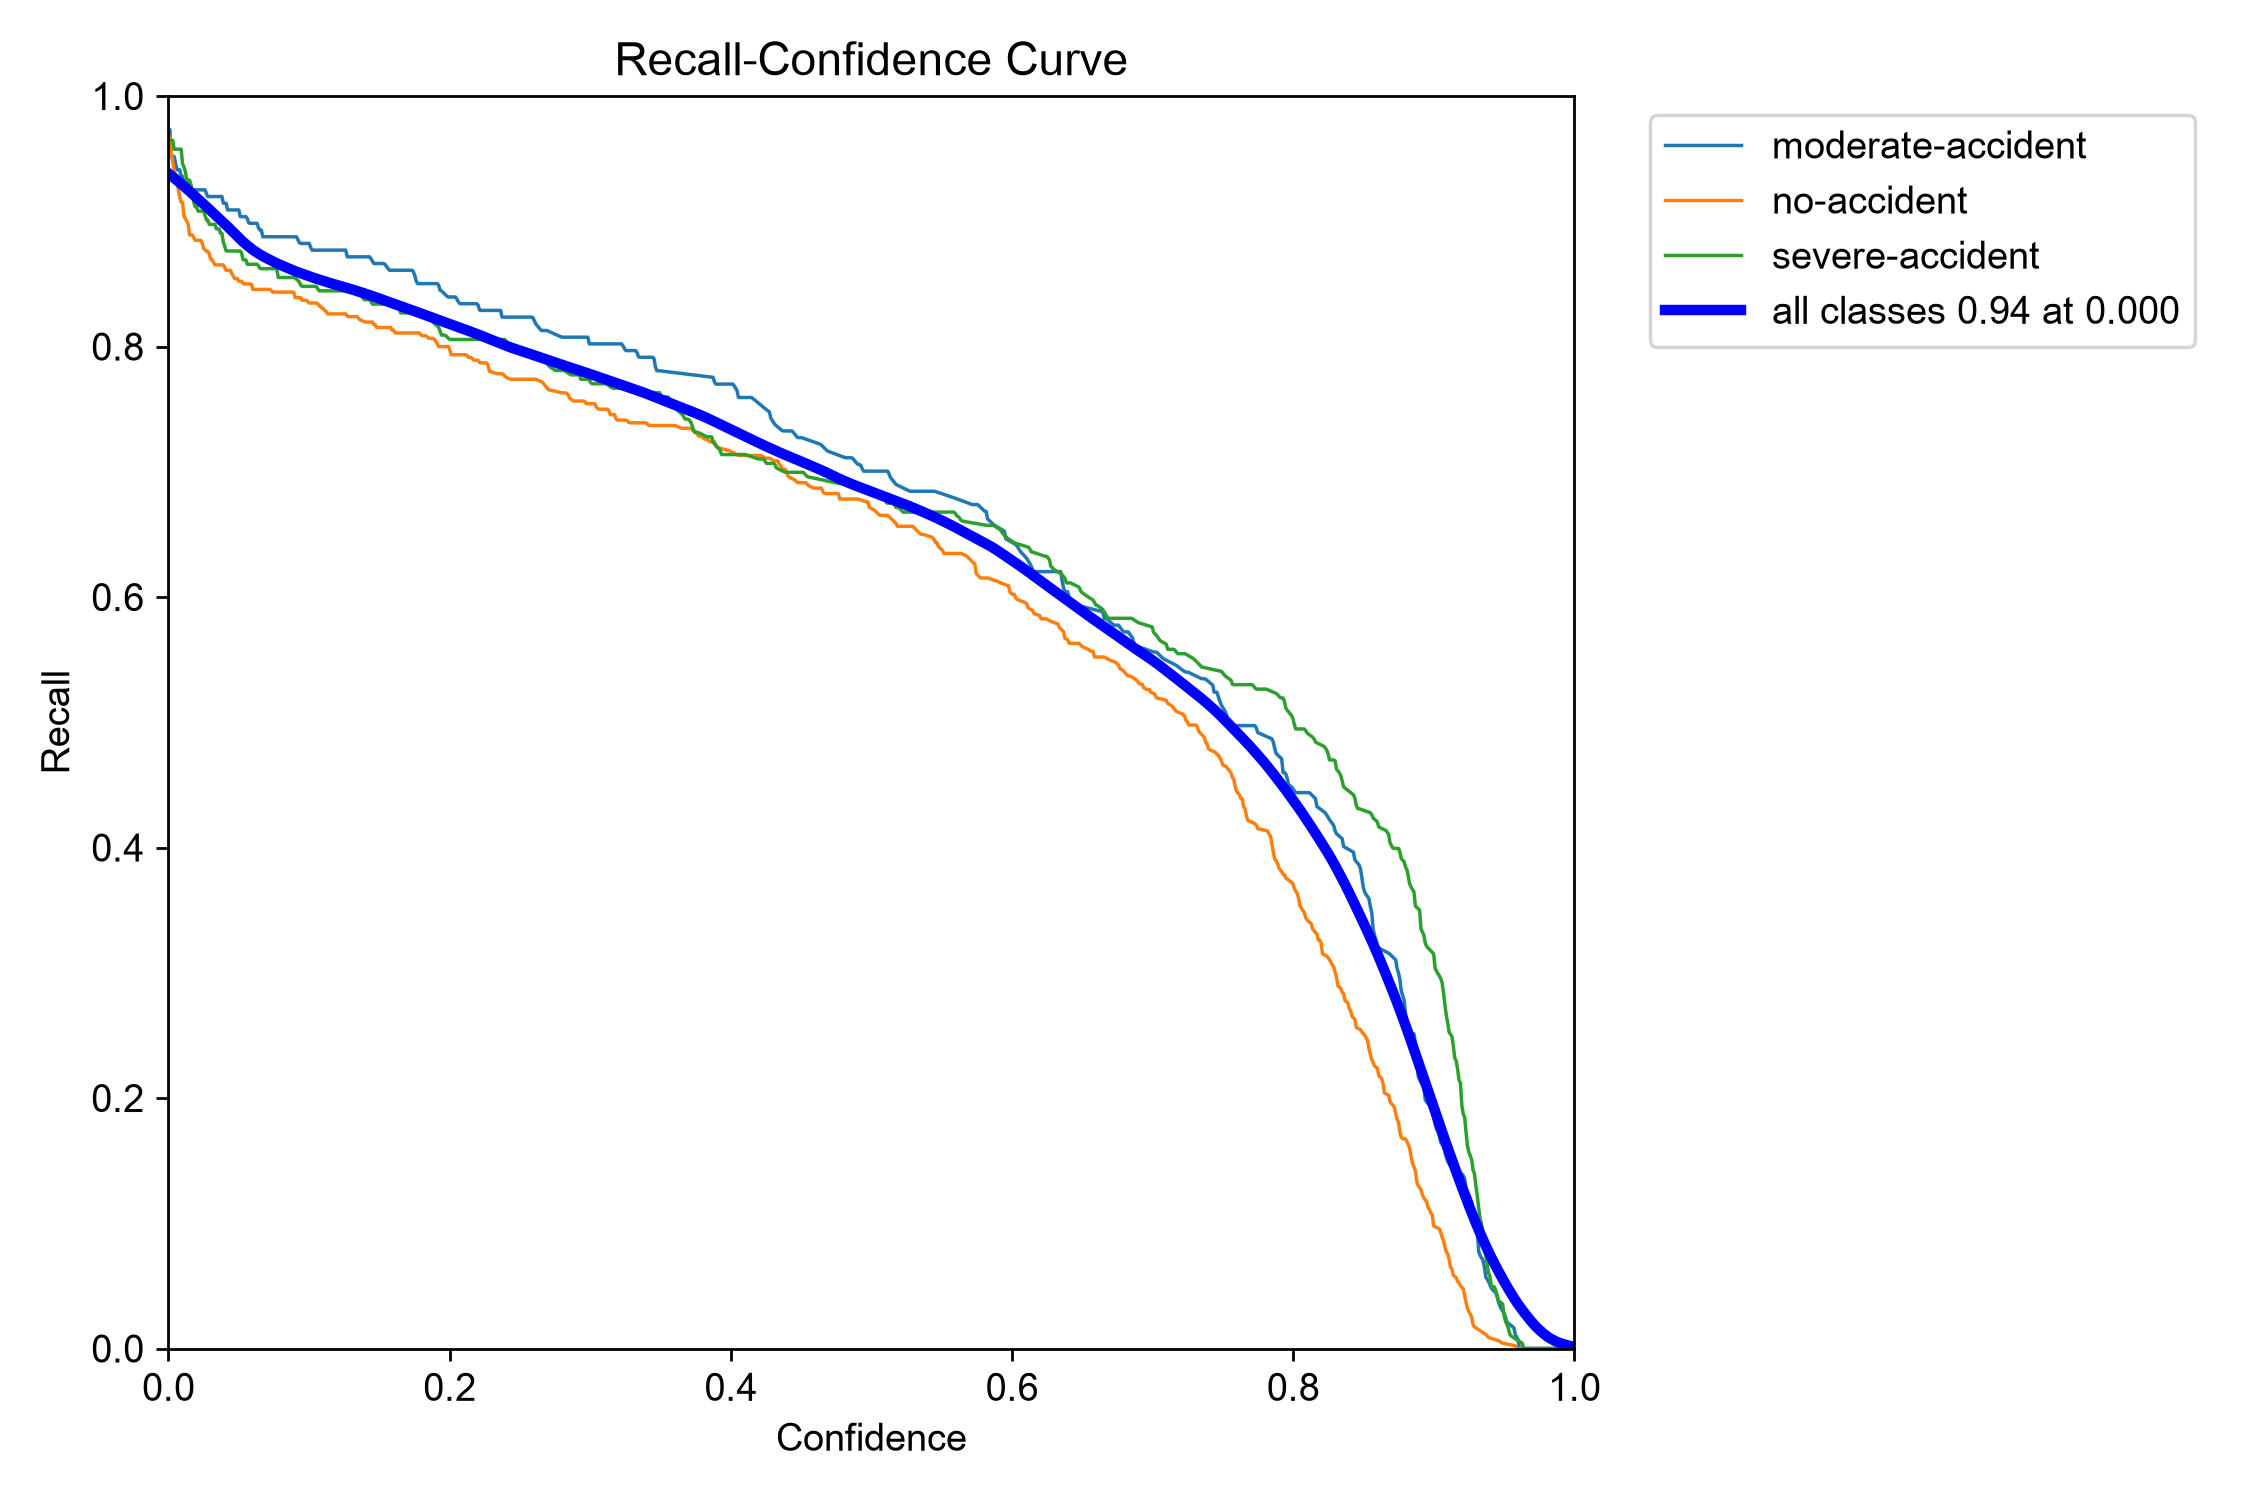
\includegraphics[width=\linewidth]{results/detection/accident_severity-2/BoxR_curve.png}\end{minipage}\hfill
\begin{minipage}{0.48\textwidth}\centering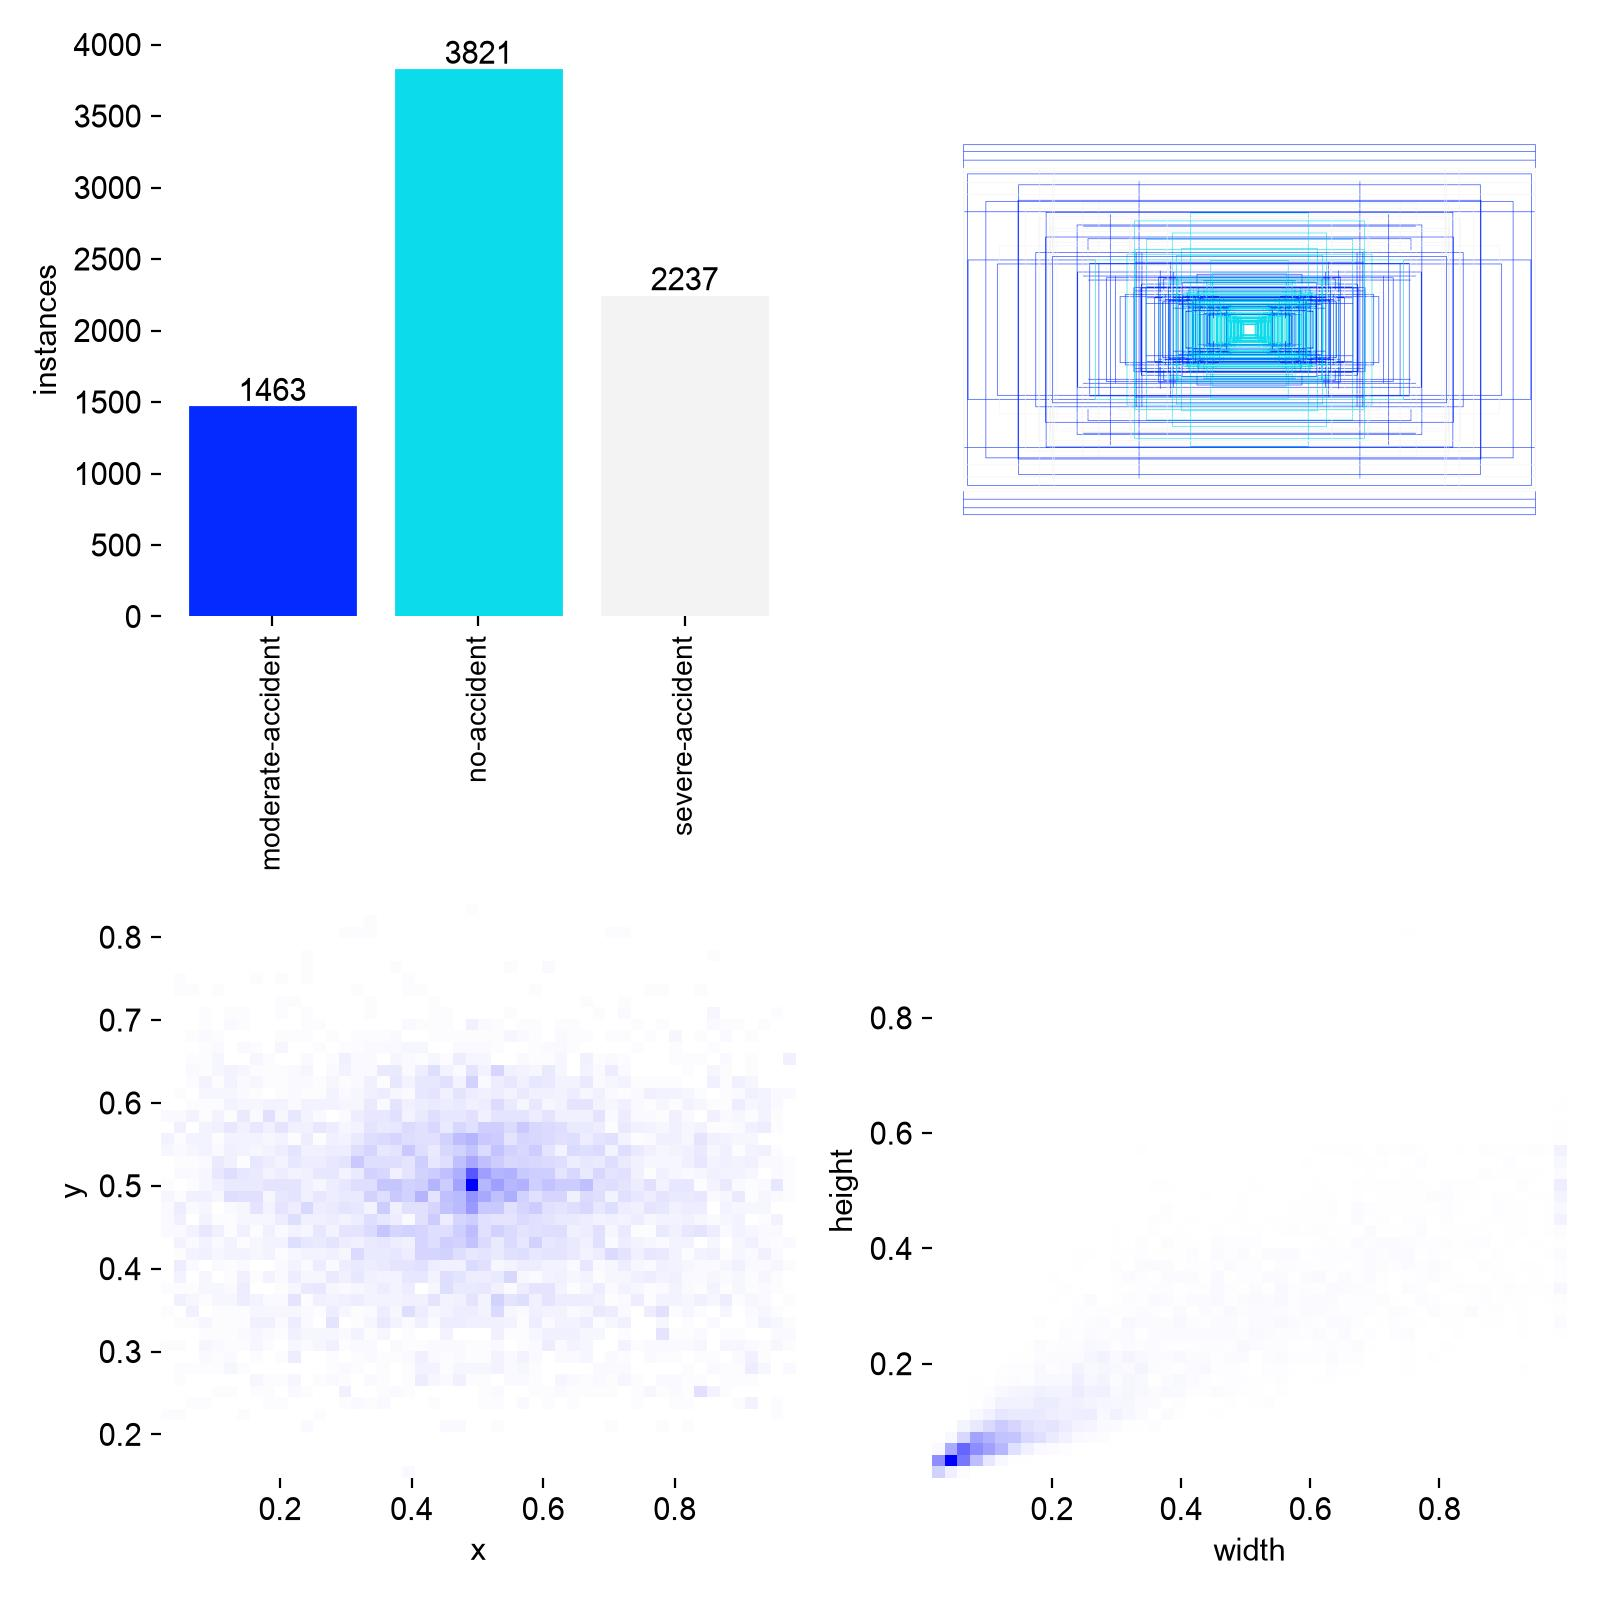
\includegraphics[width=\linewidth]{results/detection/accident_severity-2/labels.jpg}\end{minipage}
\caption{Severity-run recall curve and label-distribution summary.}
\label{fig:sev-labels}\end{figure}
\begin{figure}[t]\centering
\begin{minipage}{0.48\textwidth}\centering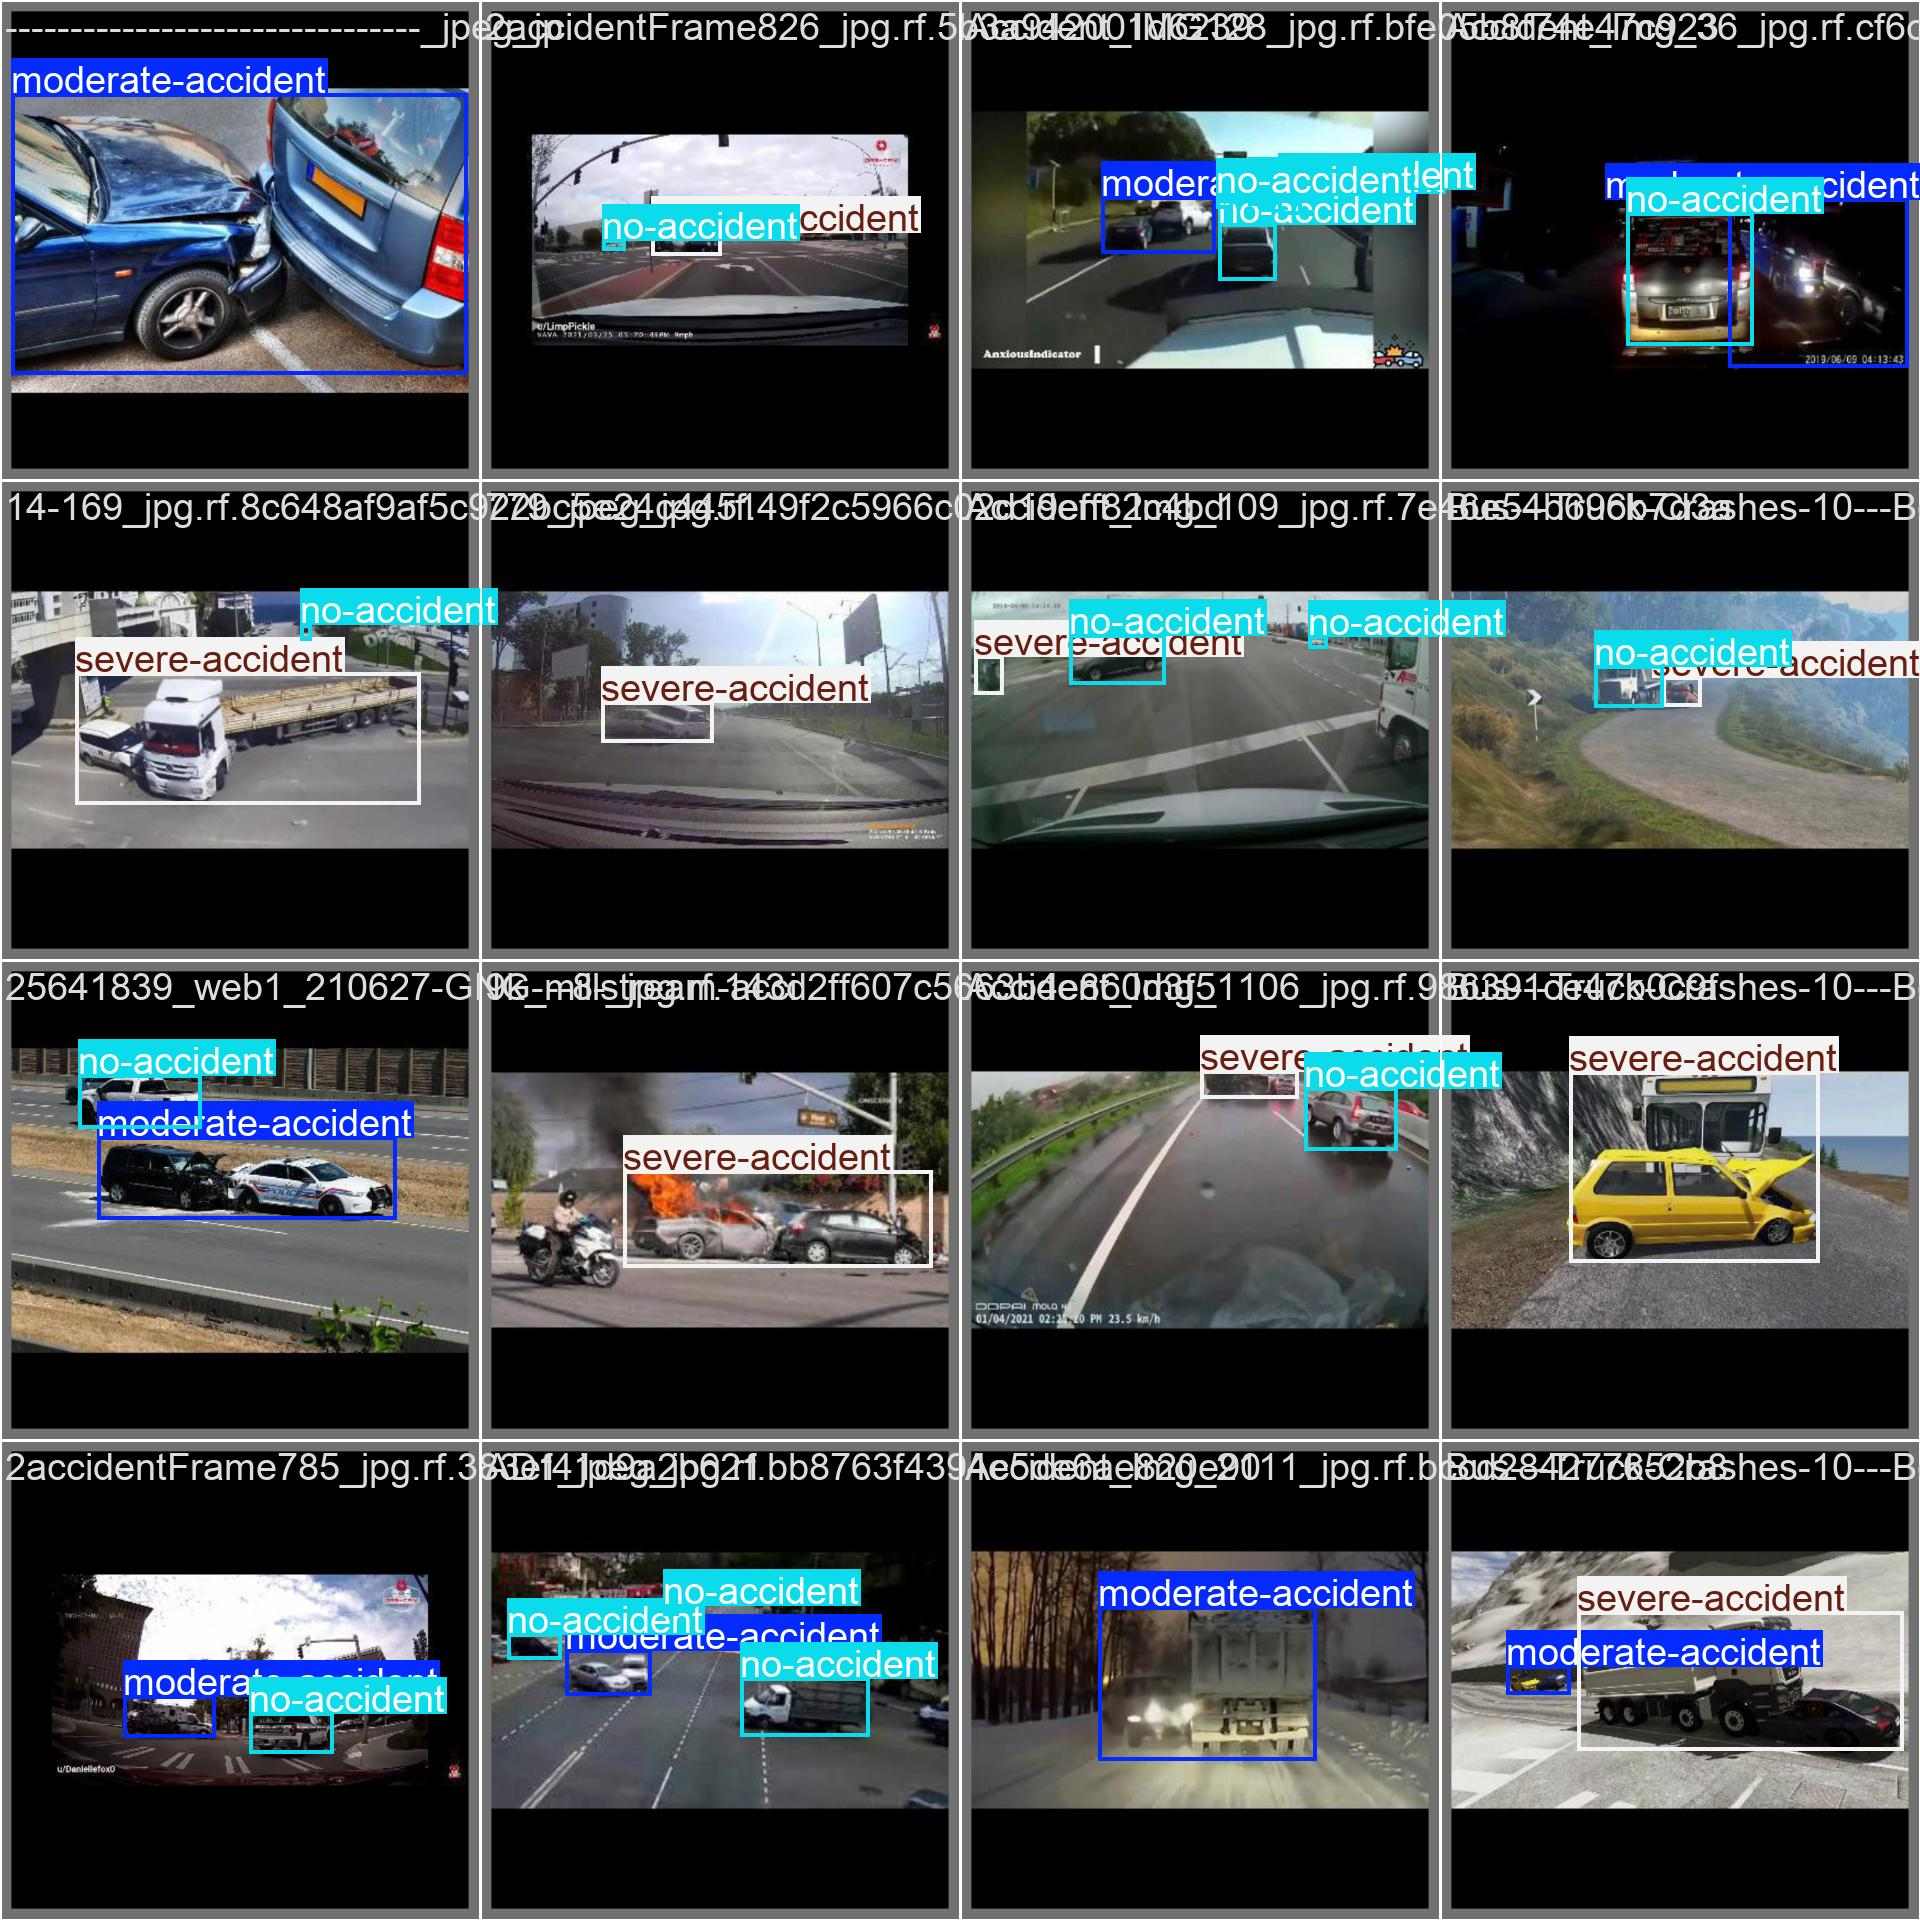
\includegraphics[width=\linewidth]{results/detection/accident_severity-2/val_batch0_labels.jpg}\end{minipage}\hfill
\begin{minipage}{0.48\textwidth}\centering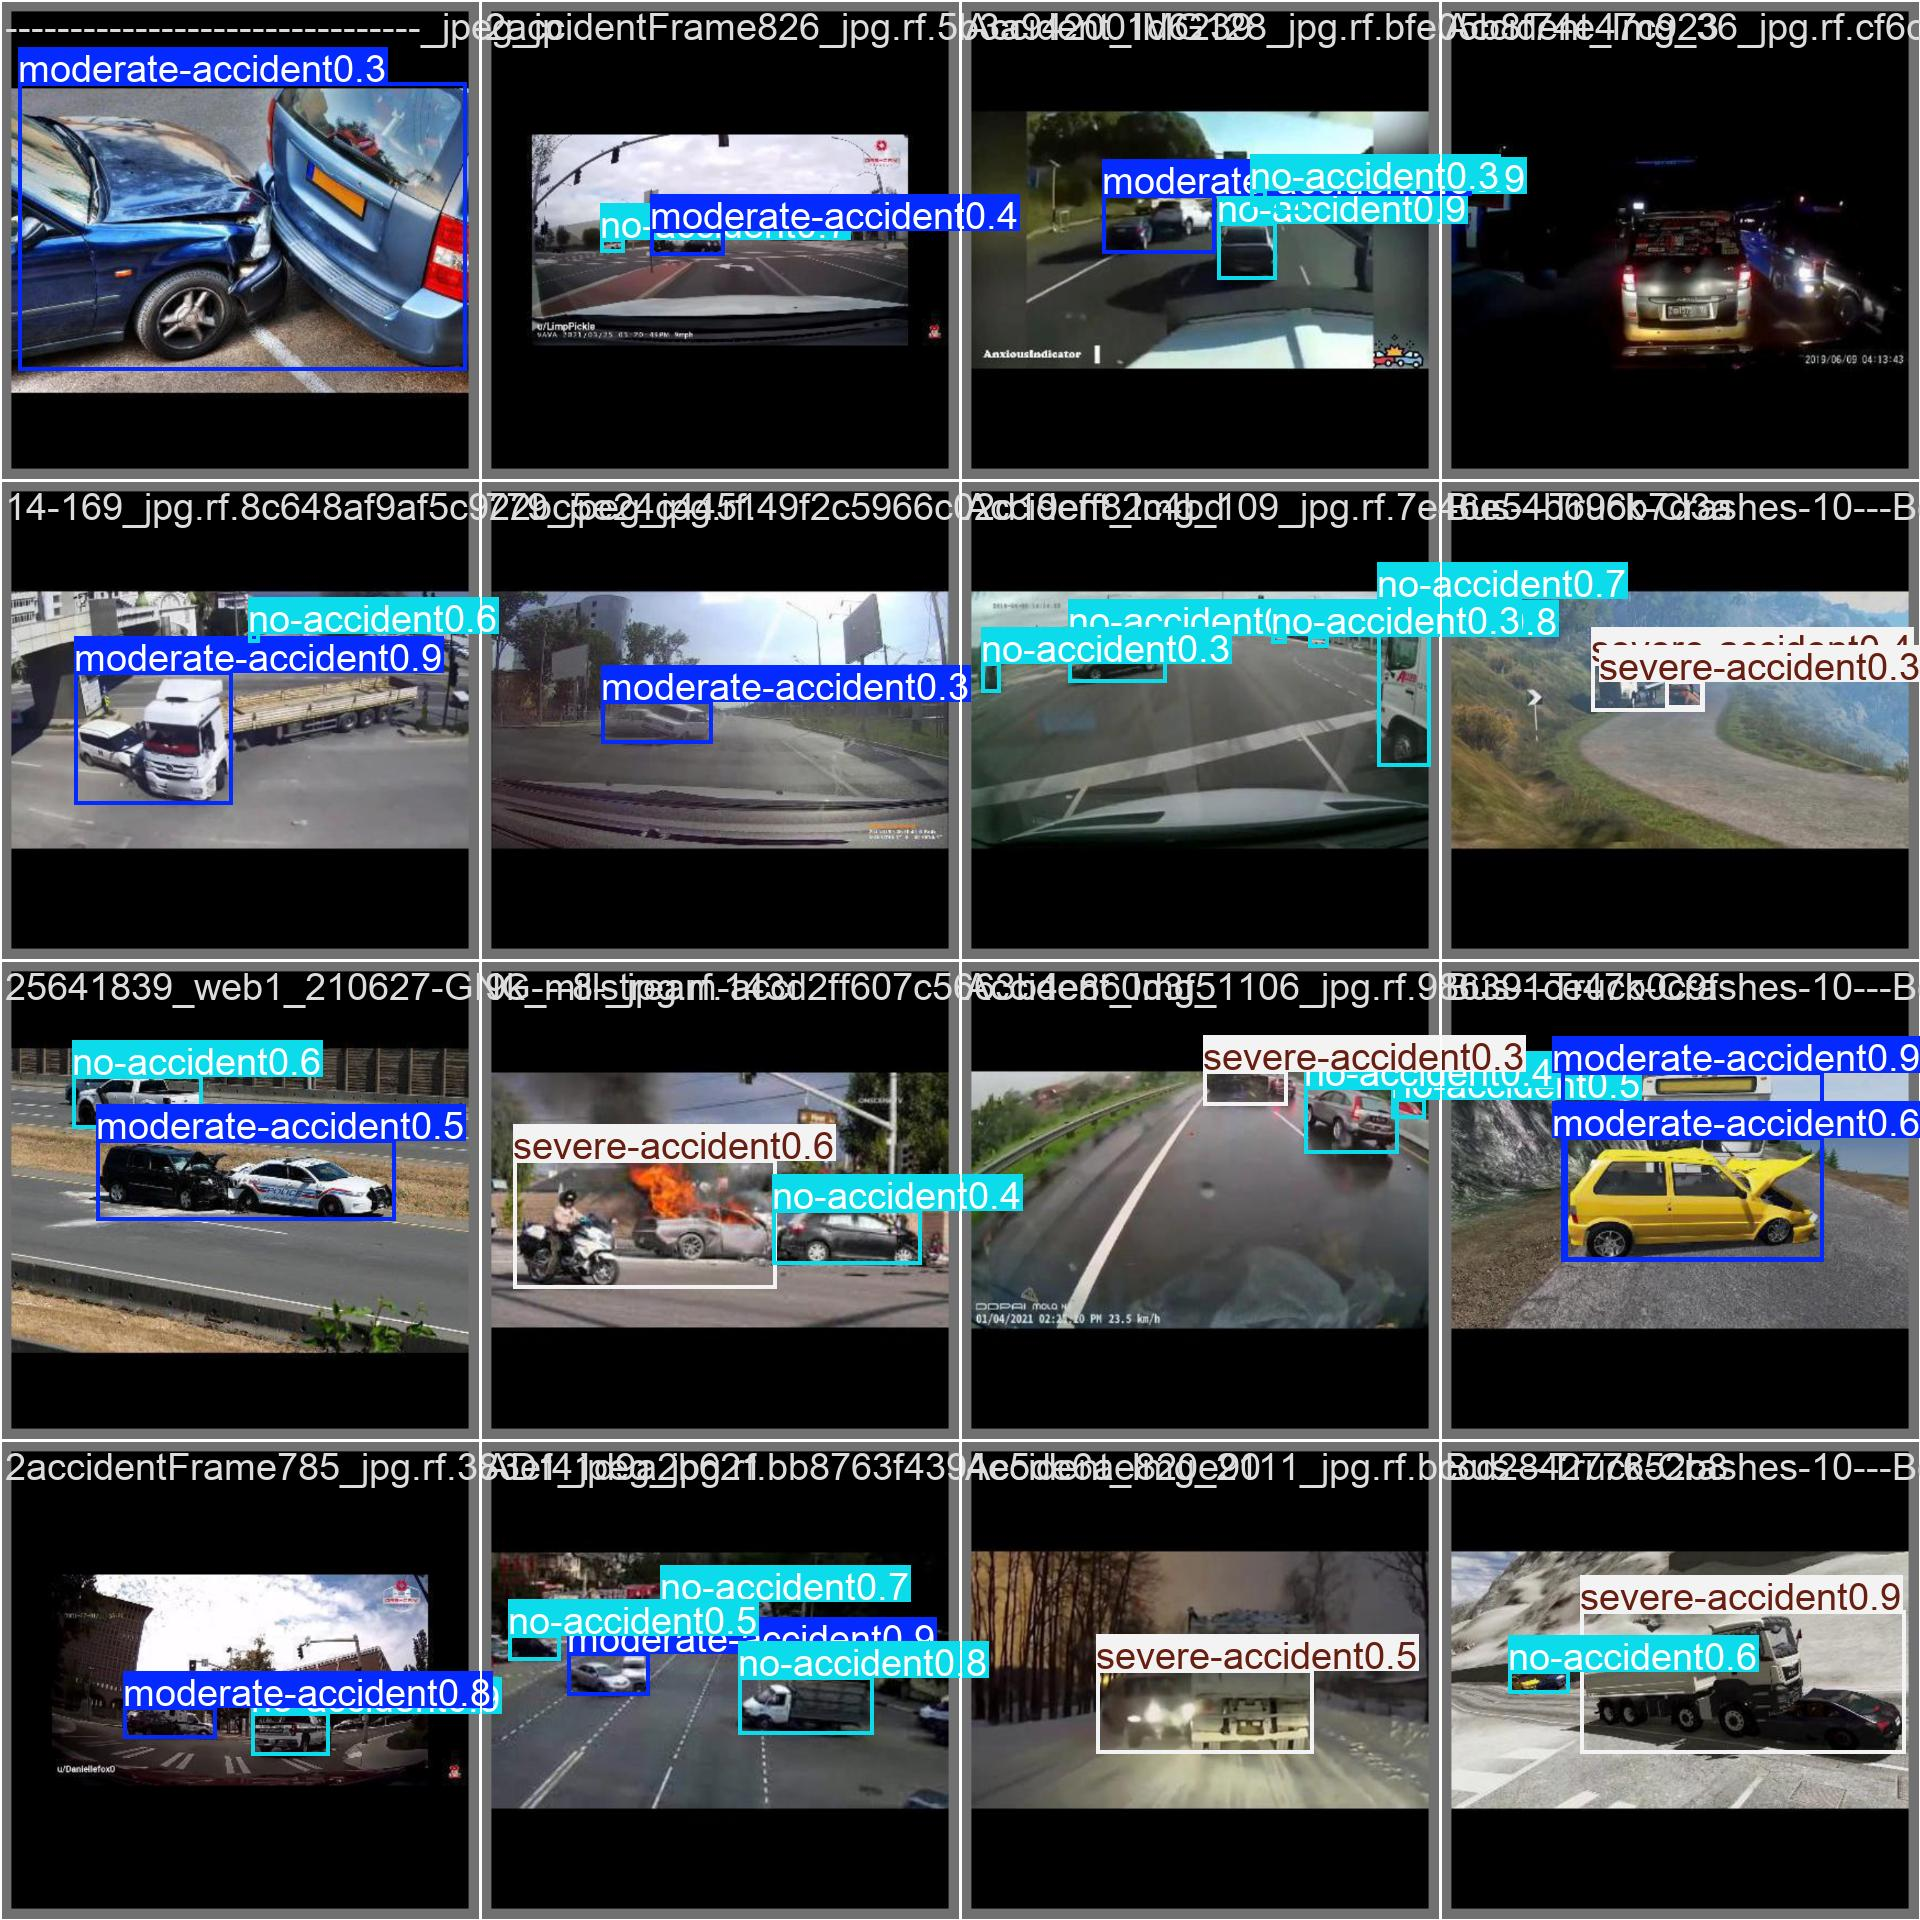
\includegraphics[width=\linewidth]{results/detection/accident_severity-2/val_batch0_pred.jpg}\end{minipage}
\caption{Representative severity validation batch: ground-truth labels and model predictions.}
\label{fig:sev-example}\end{figure}
The third model is a five-class road-user detector trained on the night-traffic collection. The final logged validation row gives 83.960\% precision, 77.684\% recall, 85.307\% mAP@0.5, and 57.371\% mAP@0.5:0.95. The mAP gap is 27.936 points. These values characterize only its configured validation split and road-user labels; they are not accident-event metrics. The saved run took approximately 20,055 seconds. Its figures are included with the supplementary run artifacts.

\begin{figure}[t]\centering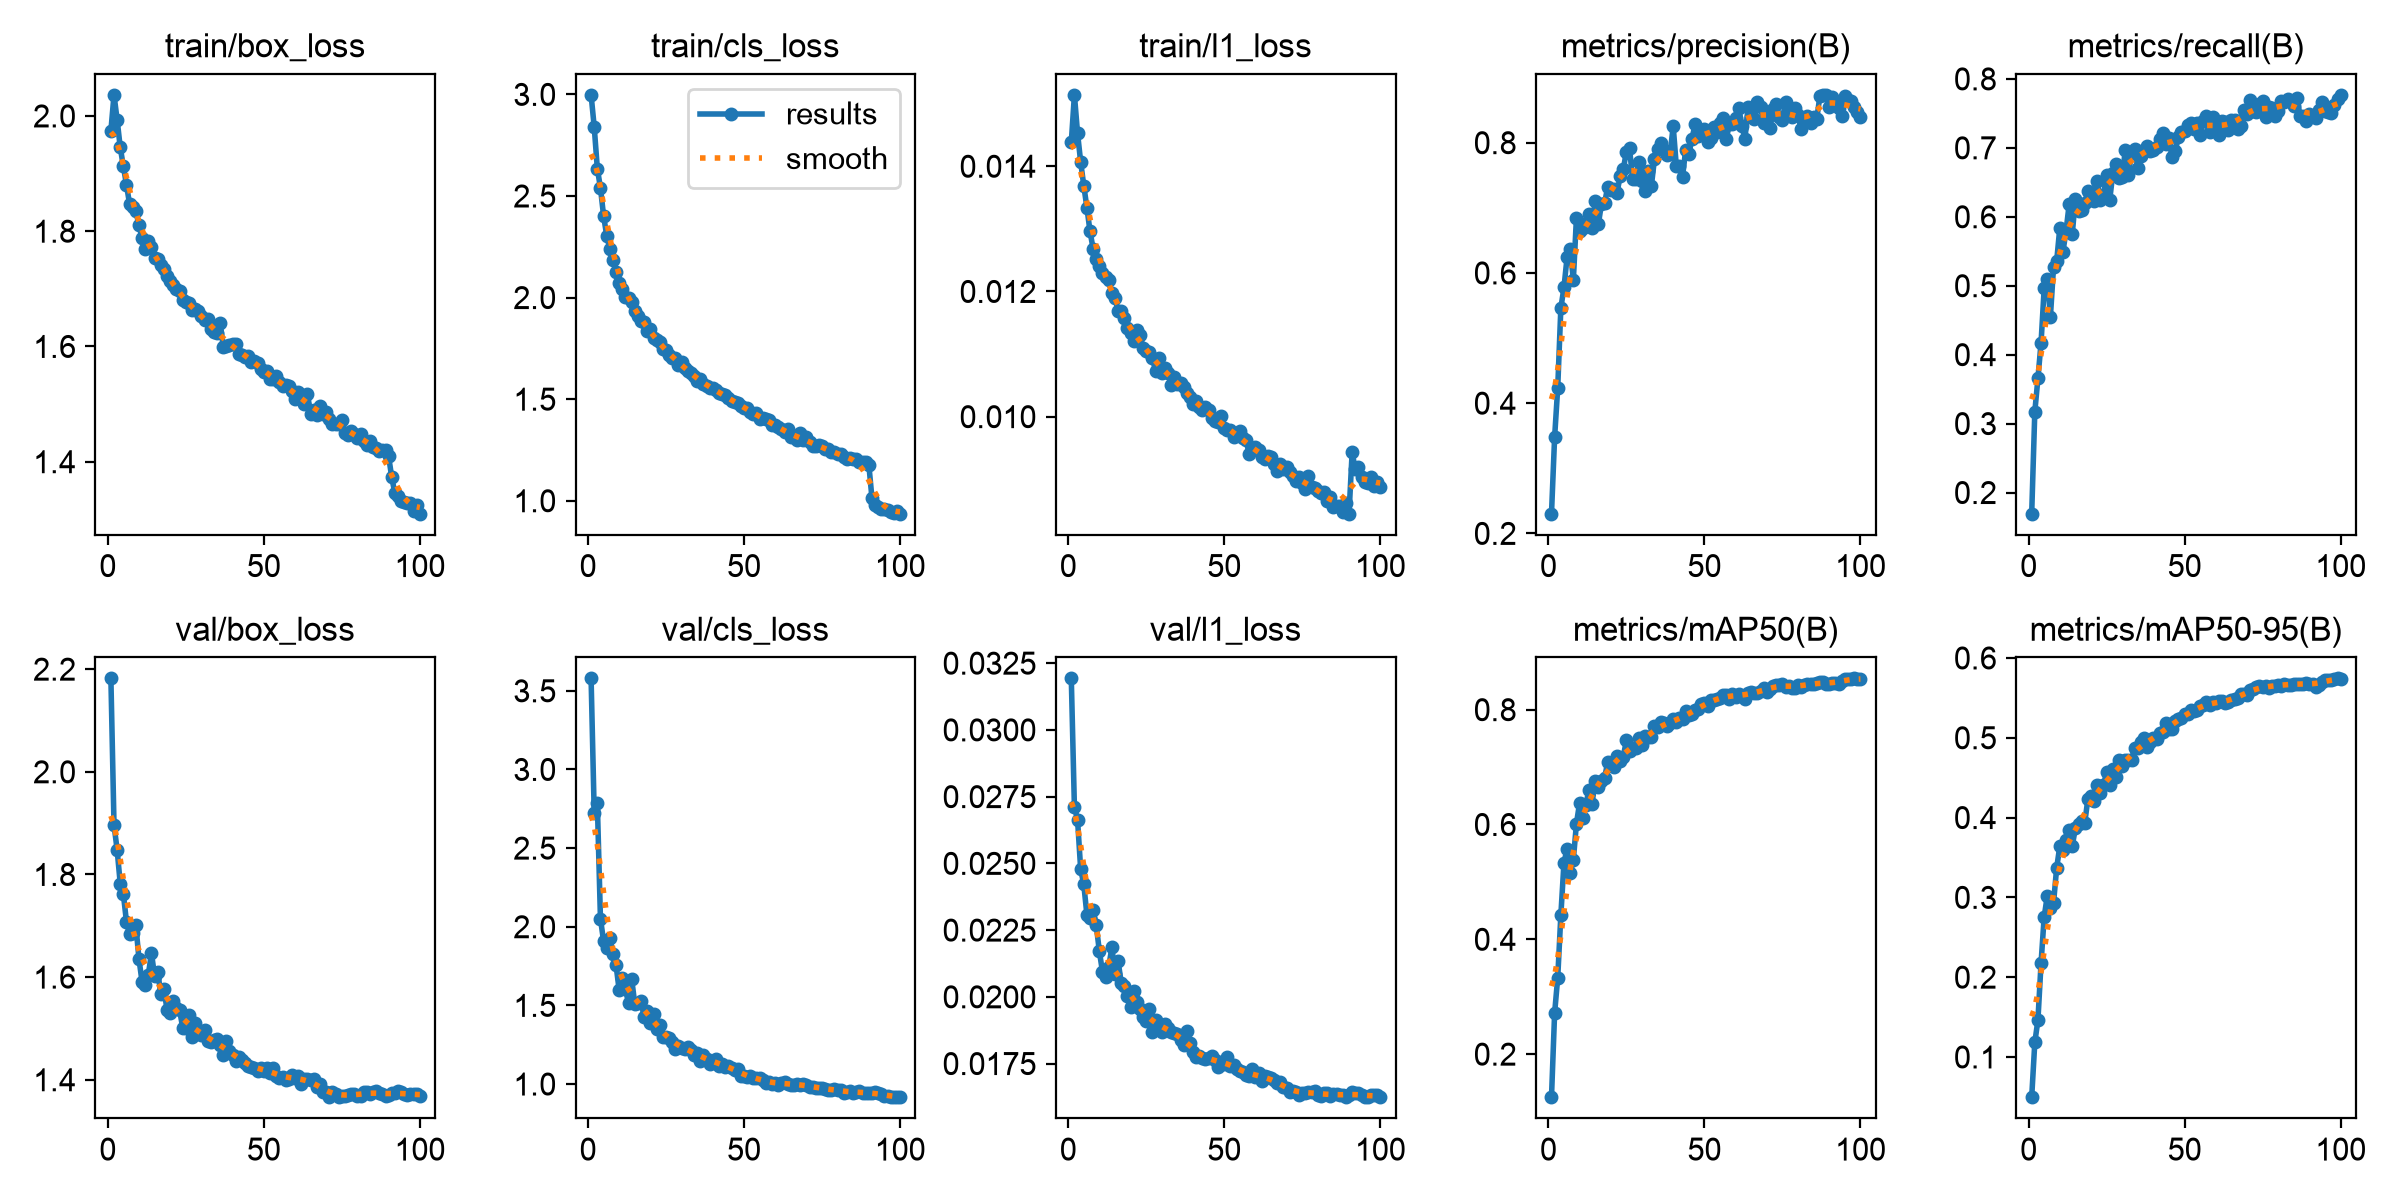
\includegraphics[width=0.92\textwidth]{results/detection/night_traffic-2/results.png}
\caption{Night-traffic run training and validation curves.}
\label{fig:nt-results}\end{figure}
\begin{figure}[t]\centering
\begin{minipage}{0.48\textwidth}\centering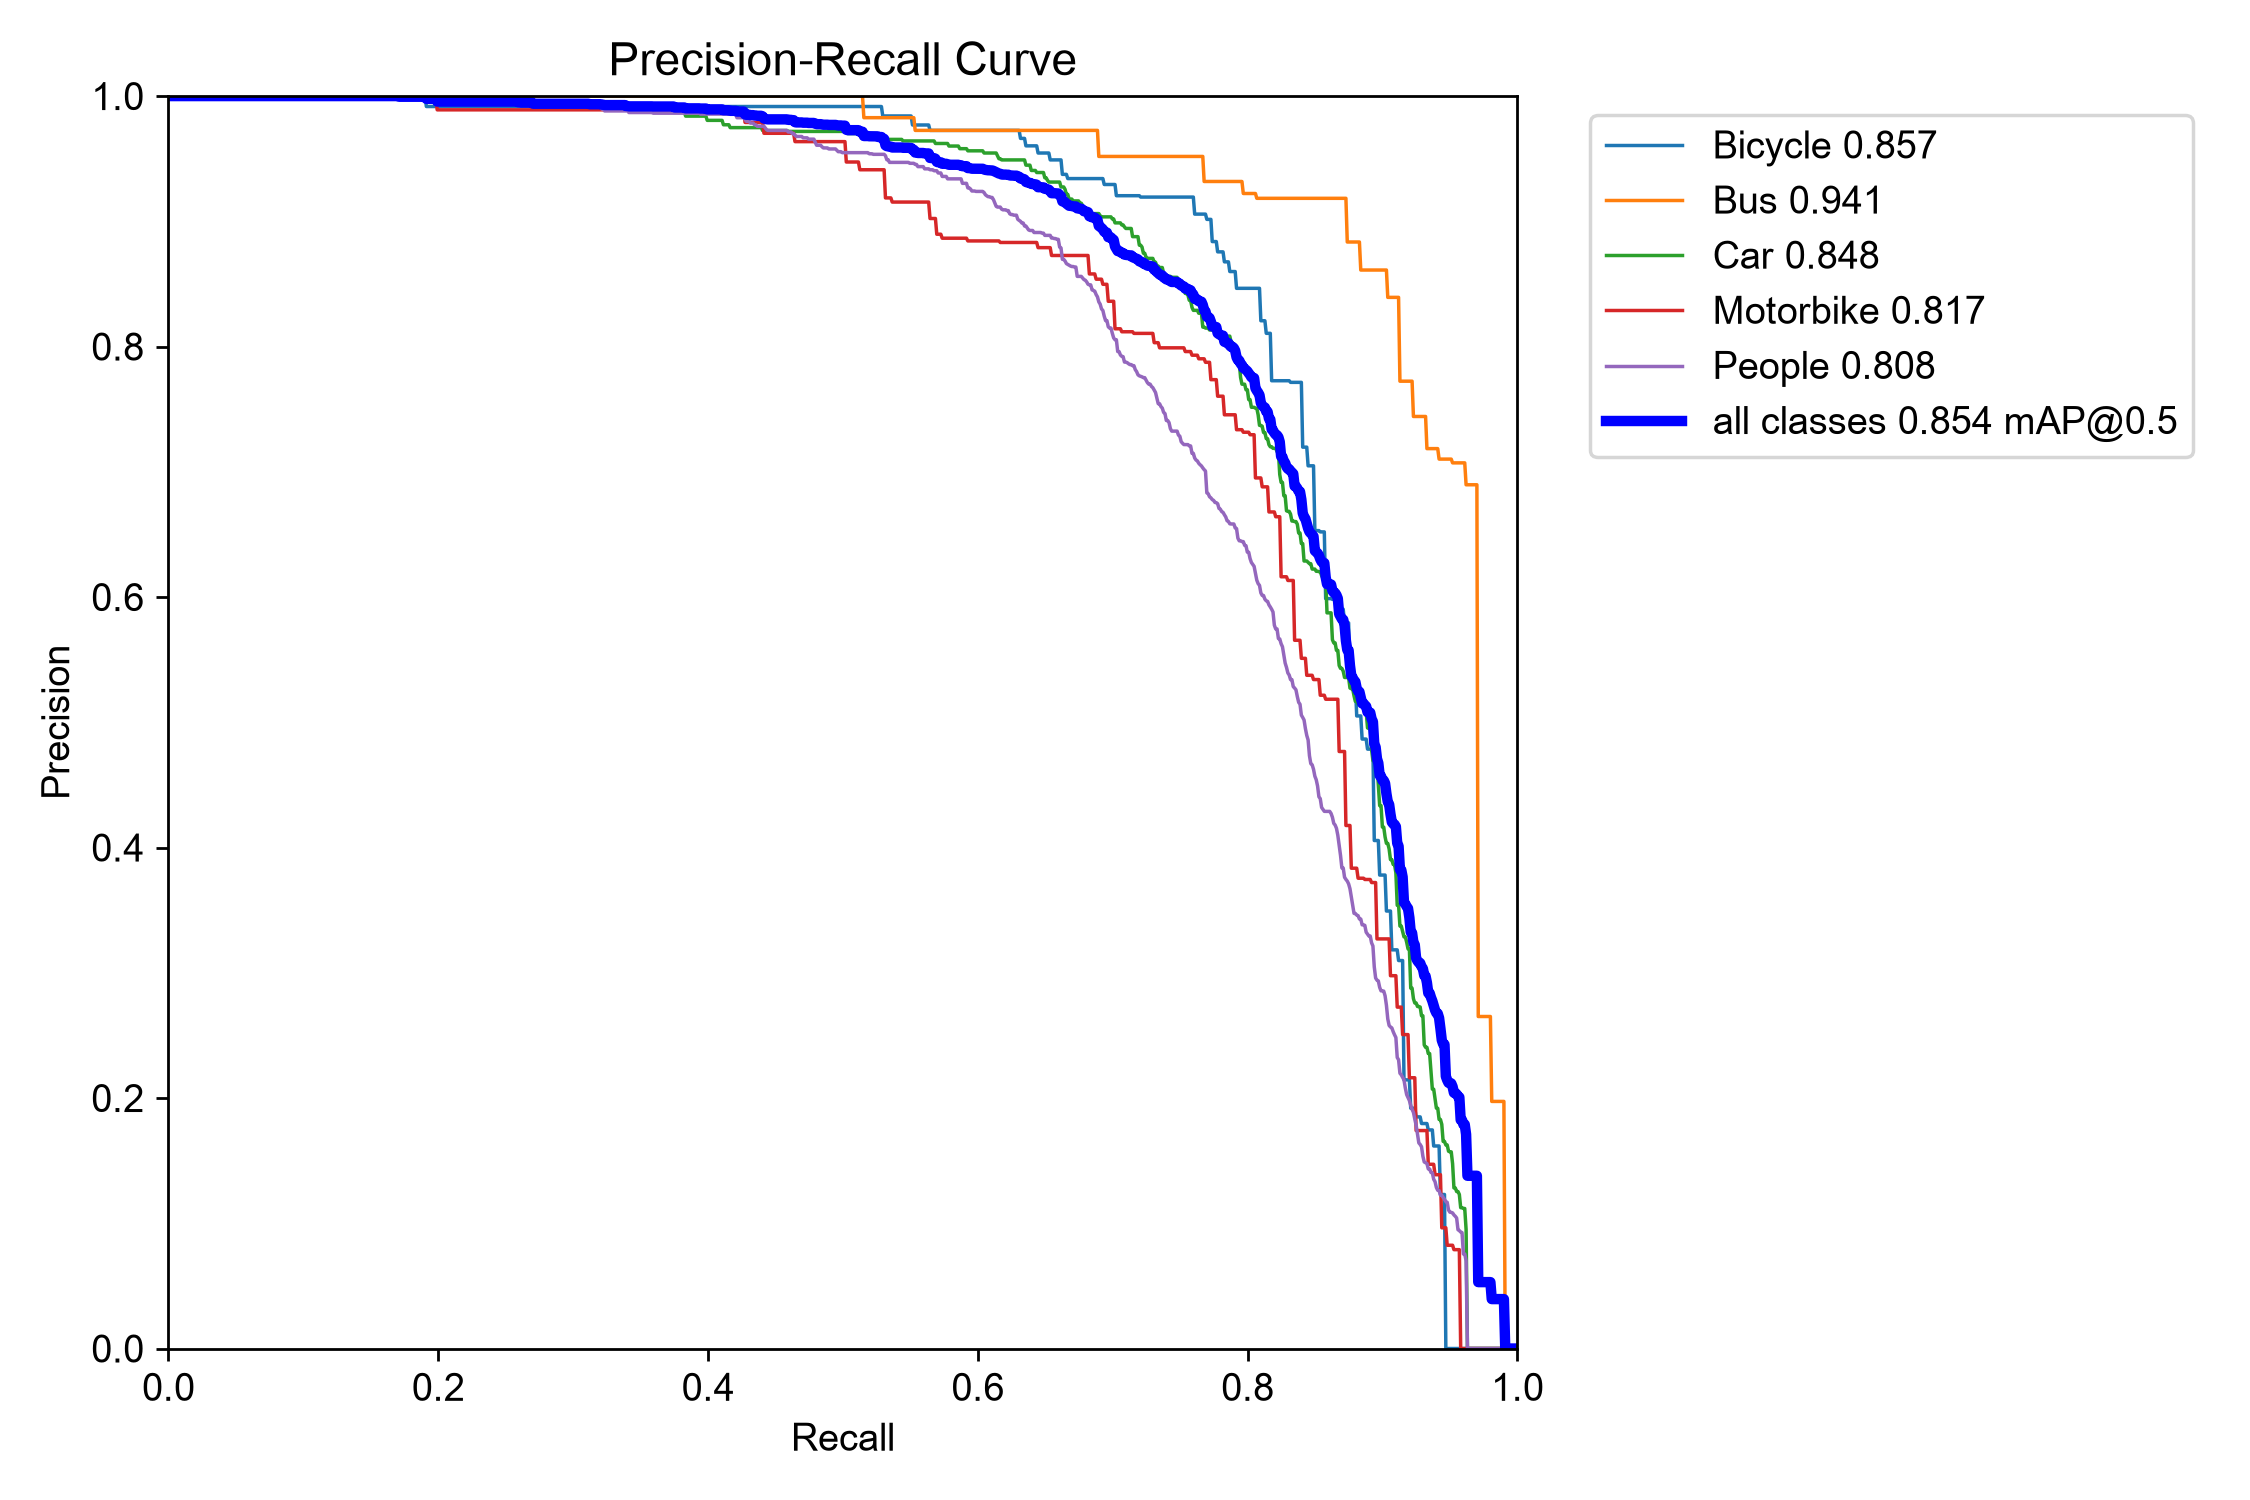
\includegraphics[width=\linewidth]{results/detection/night_traffic-2/BoxPR_curve.png}\end{minipage}\hfill
\begin{minipage}{0.48\textwidth}\centering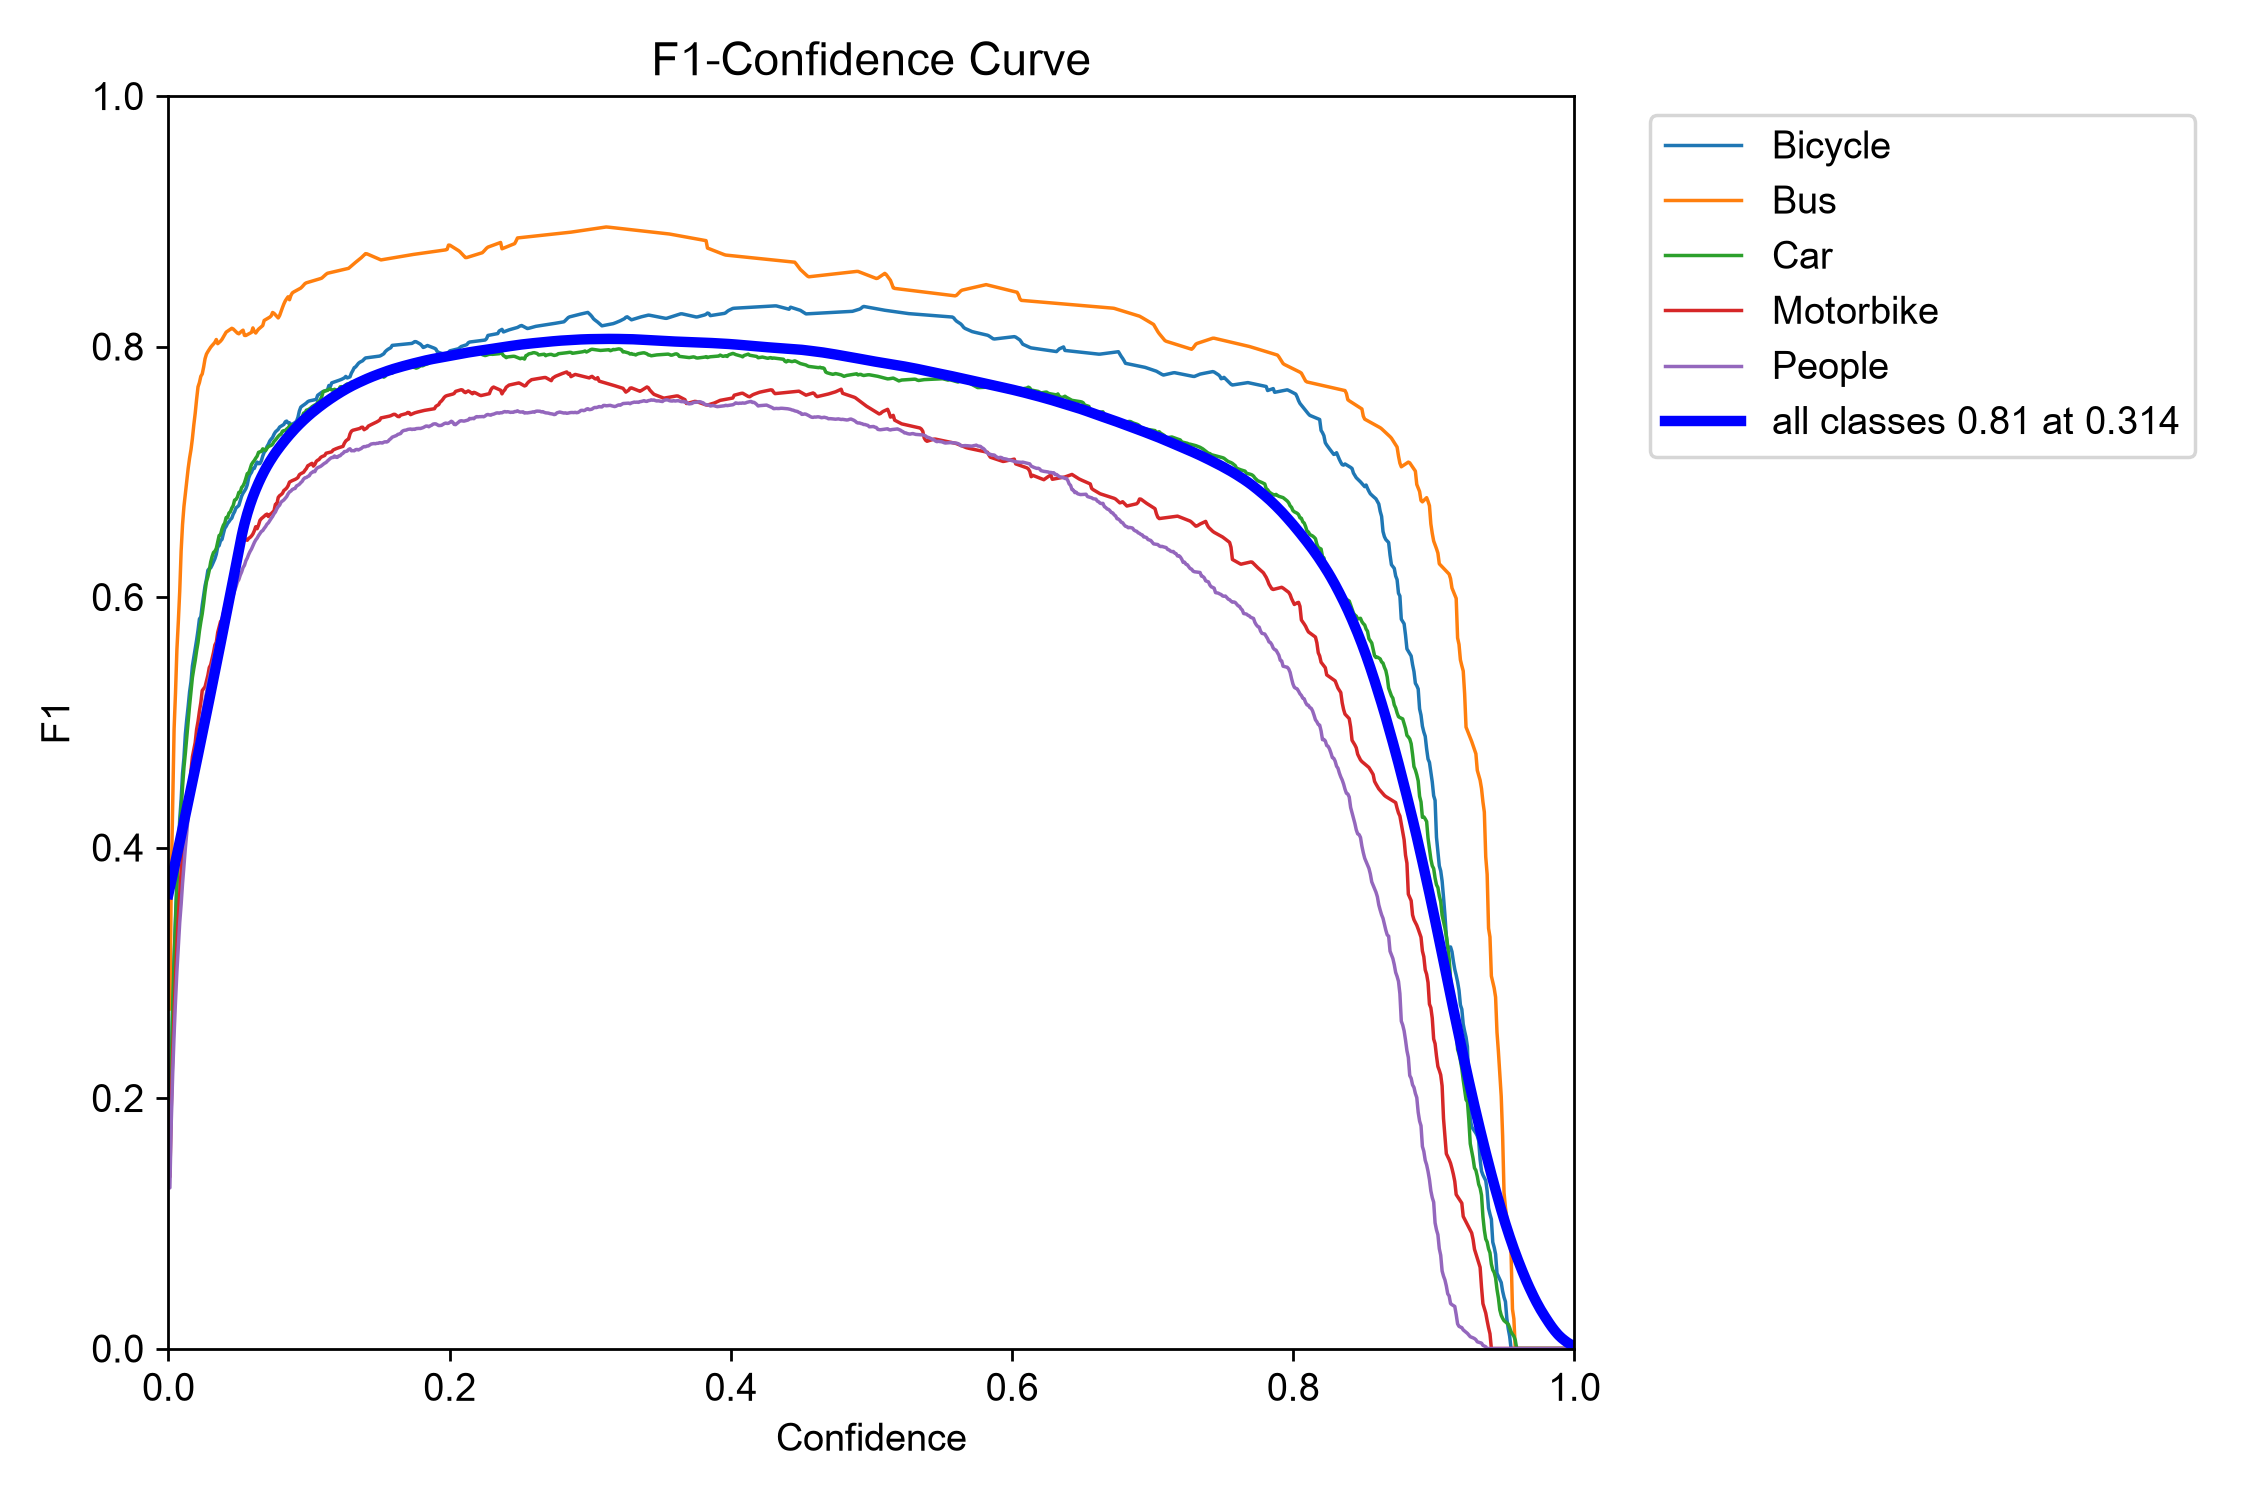
\includegraphics[width=\linewidth]{results/detection/night_traffic-2/BoxF1_curve.png}\end{minipage}
\caption{Night-traffic precision-recall and confidence-dependent F1 curves.}
\label{fig:nt-prf1}\end{figure}
\begin{figure}[t]\centering
\begin{minipage}{0.48\textwidth}\centering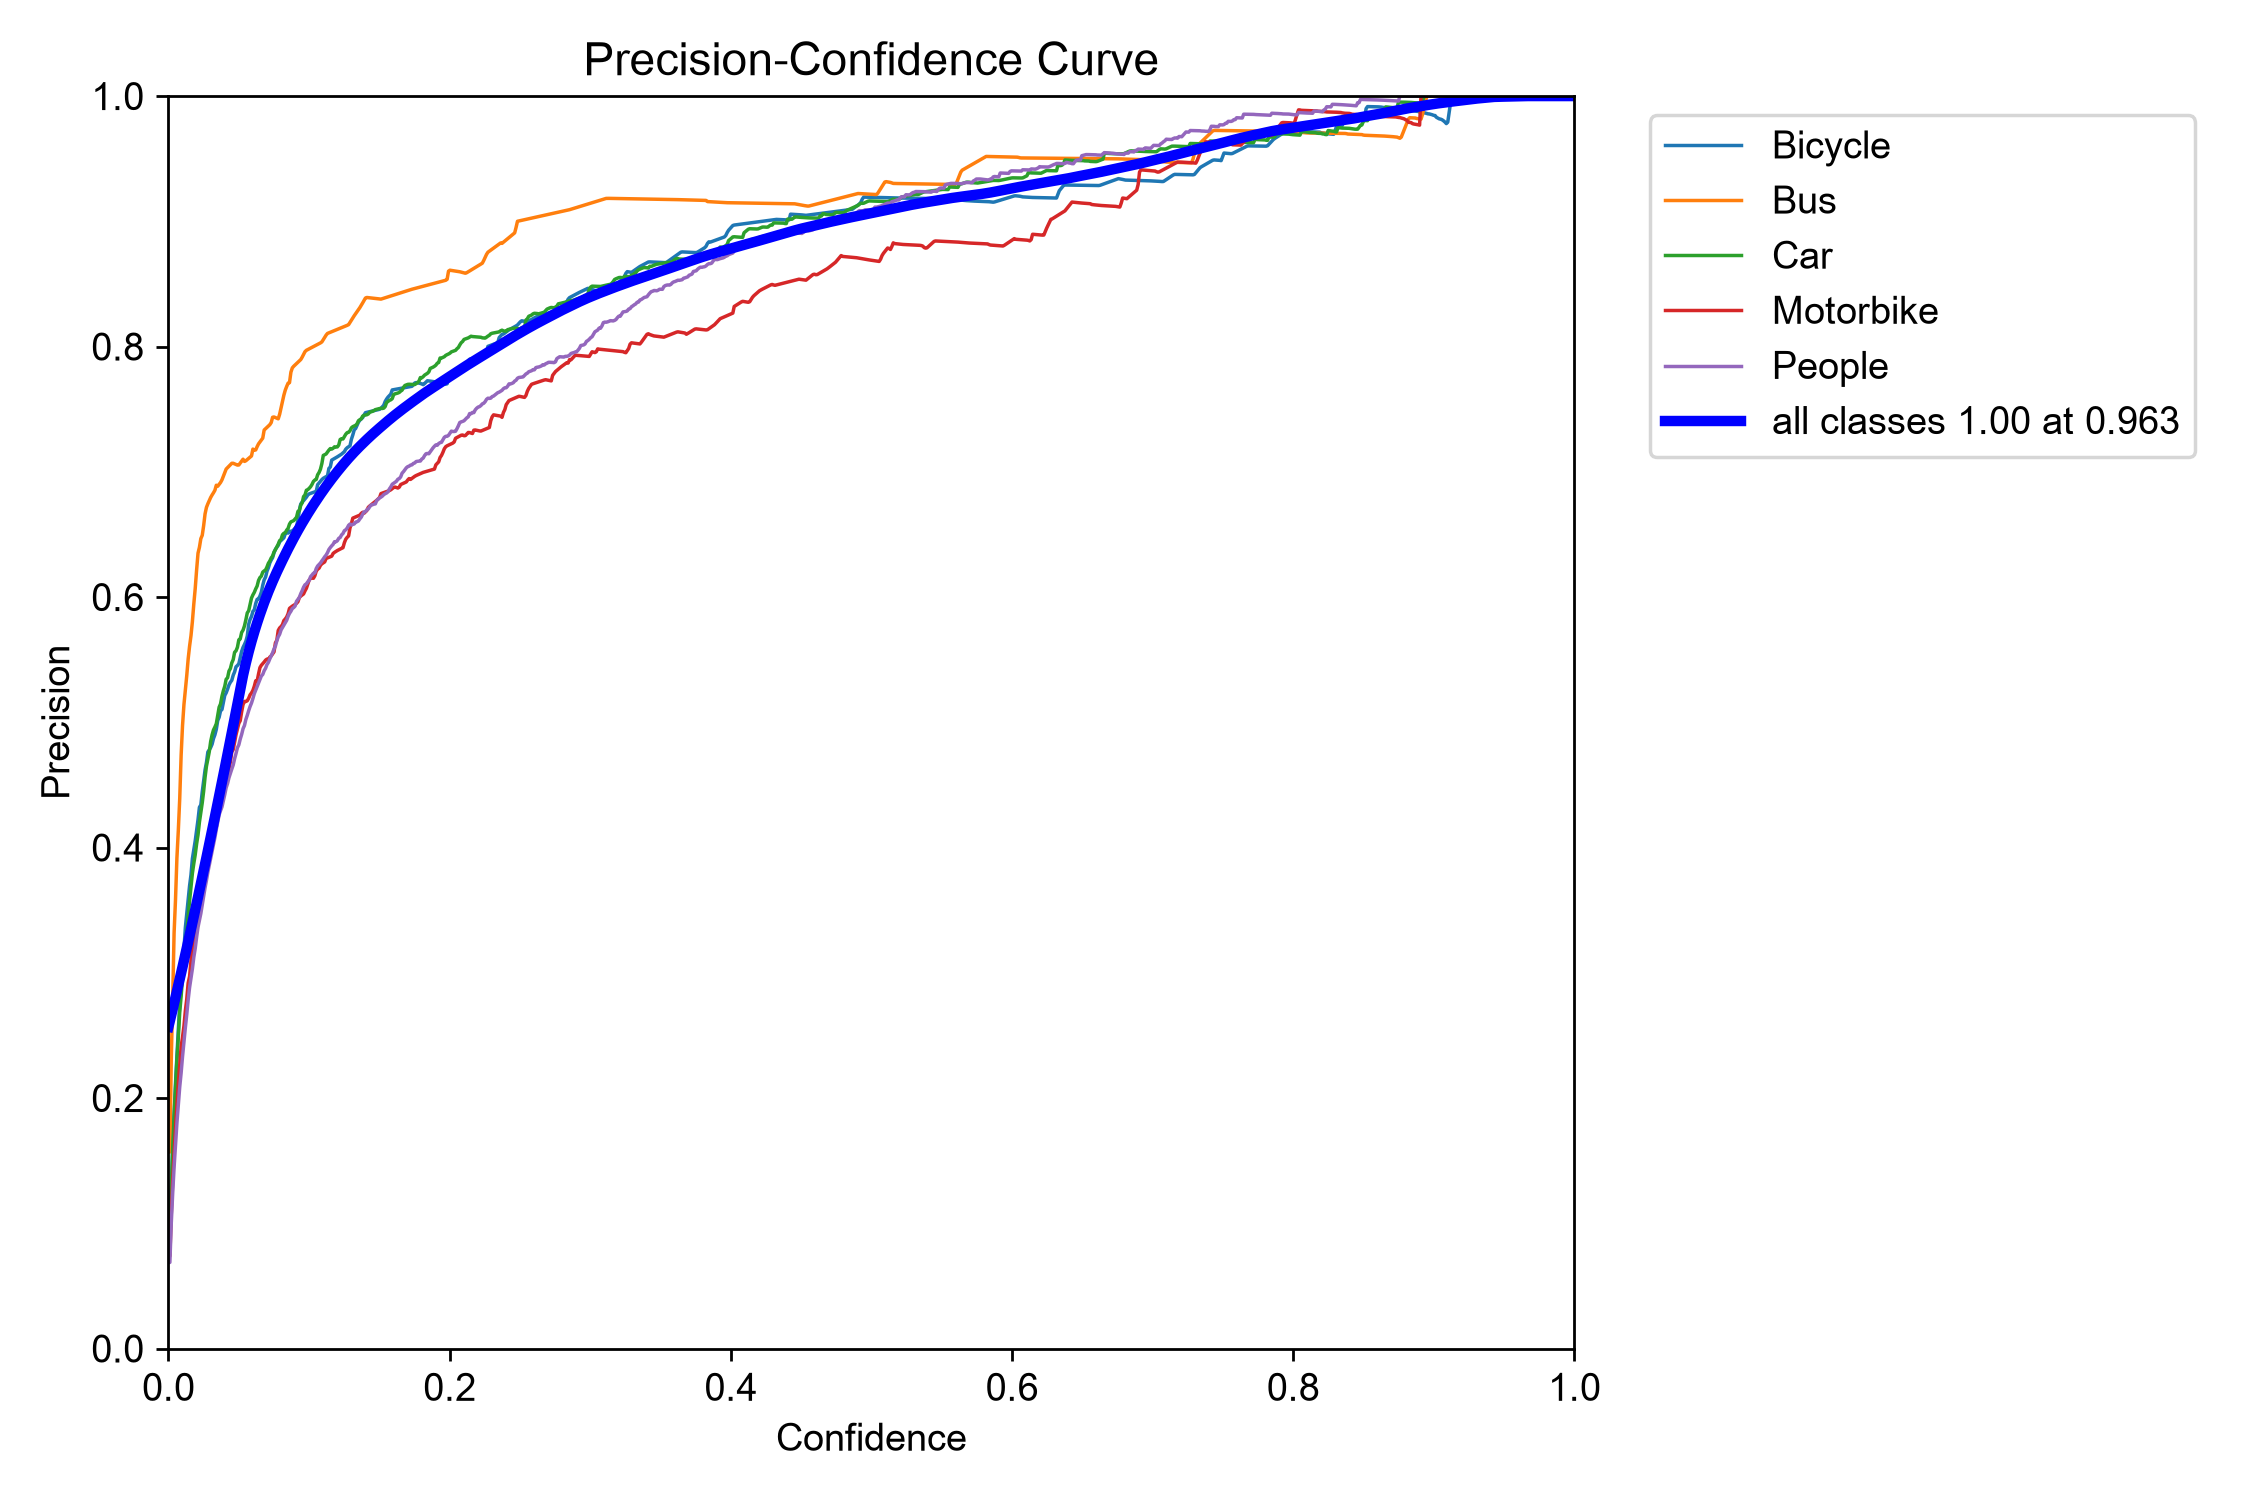
\includegraphics[width=\linewidth]{results/detection/night_traffic-2/BoxP_curve.png}\end{minipage}\hfill
\begin{minipage}{0.48\textwidth}\centering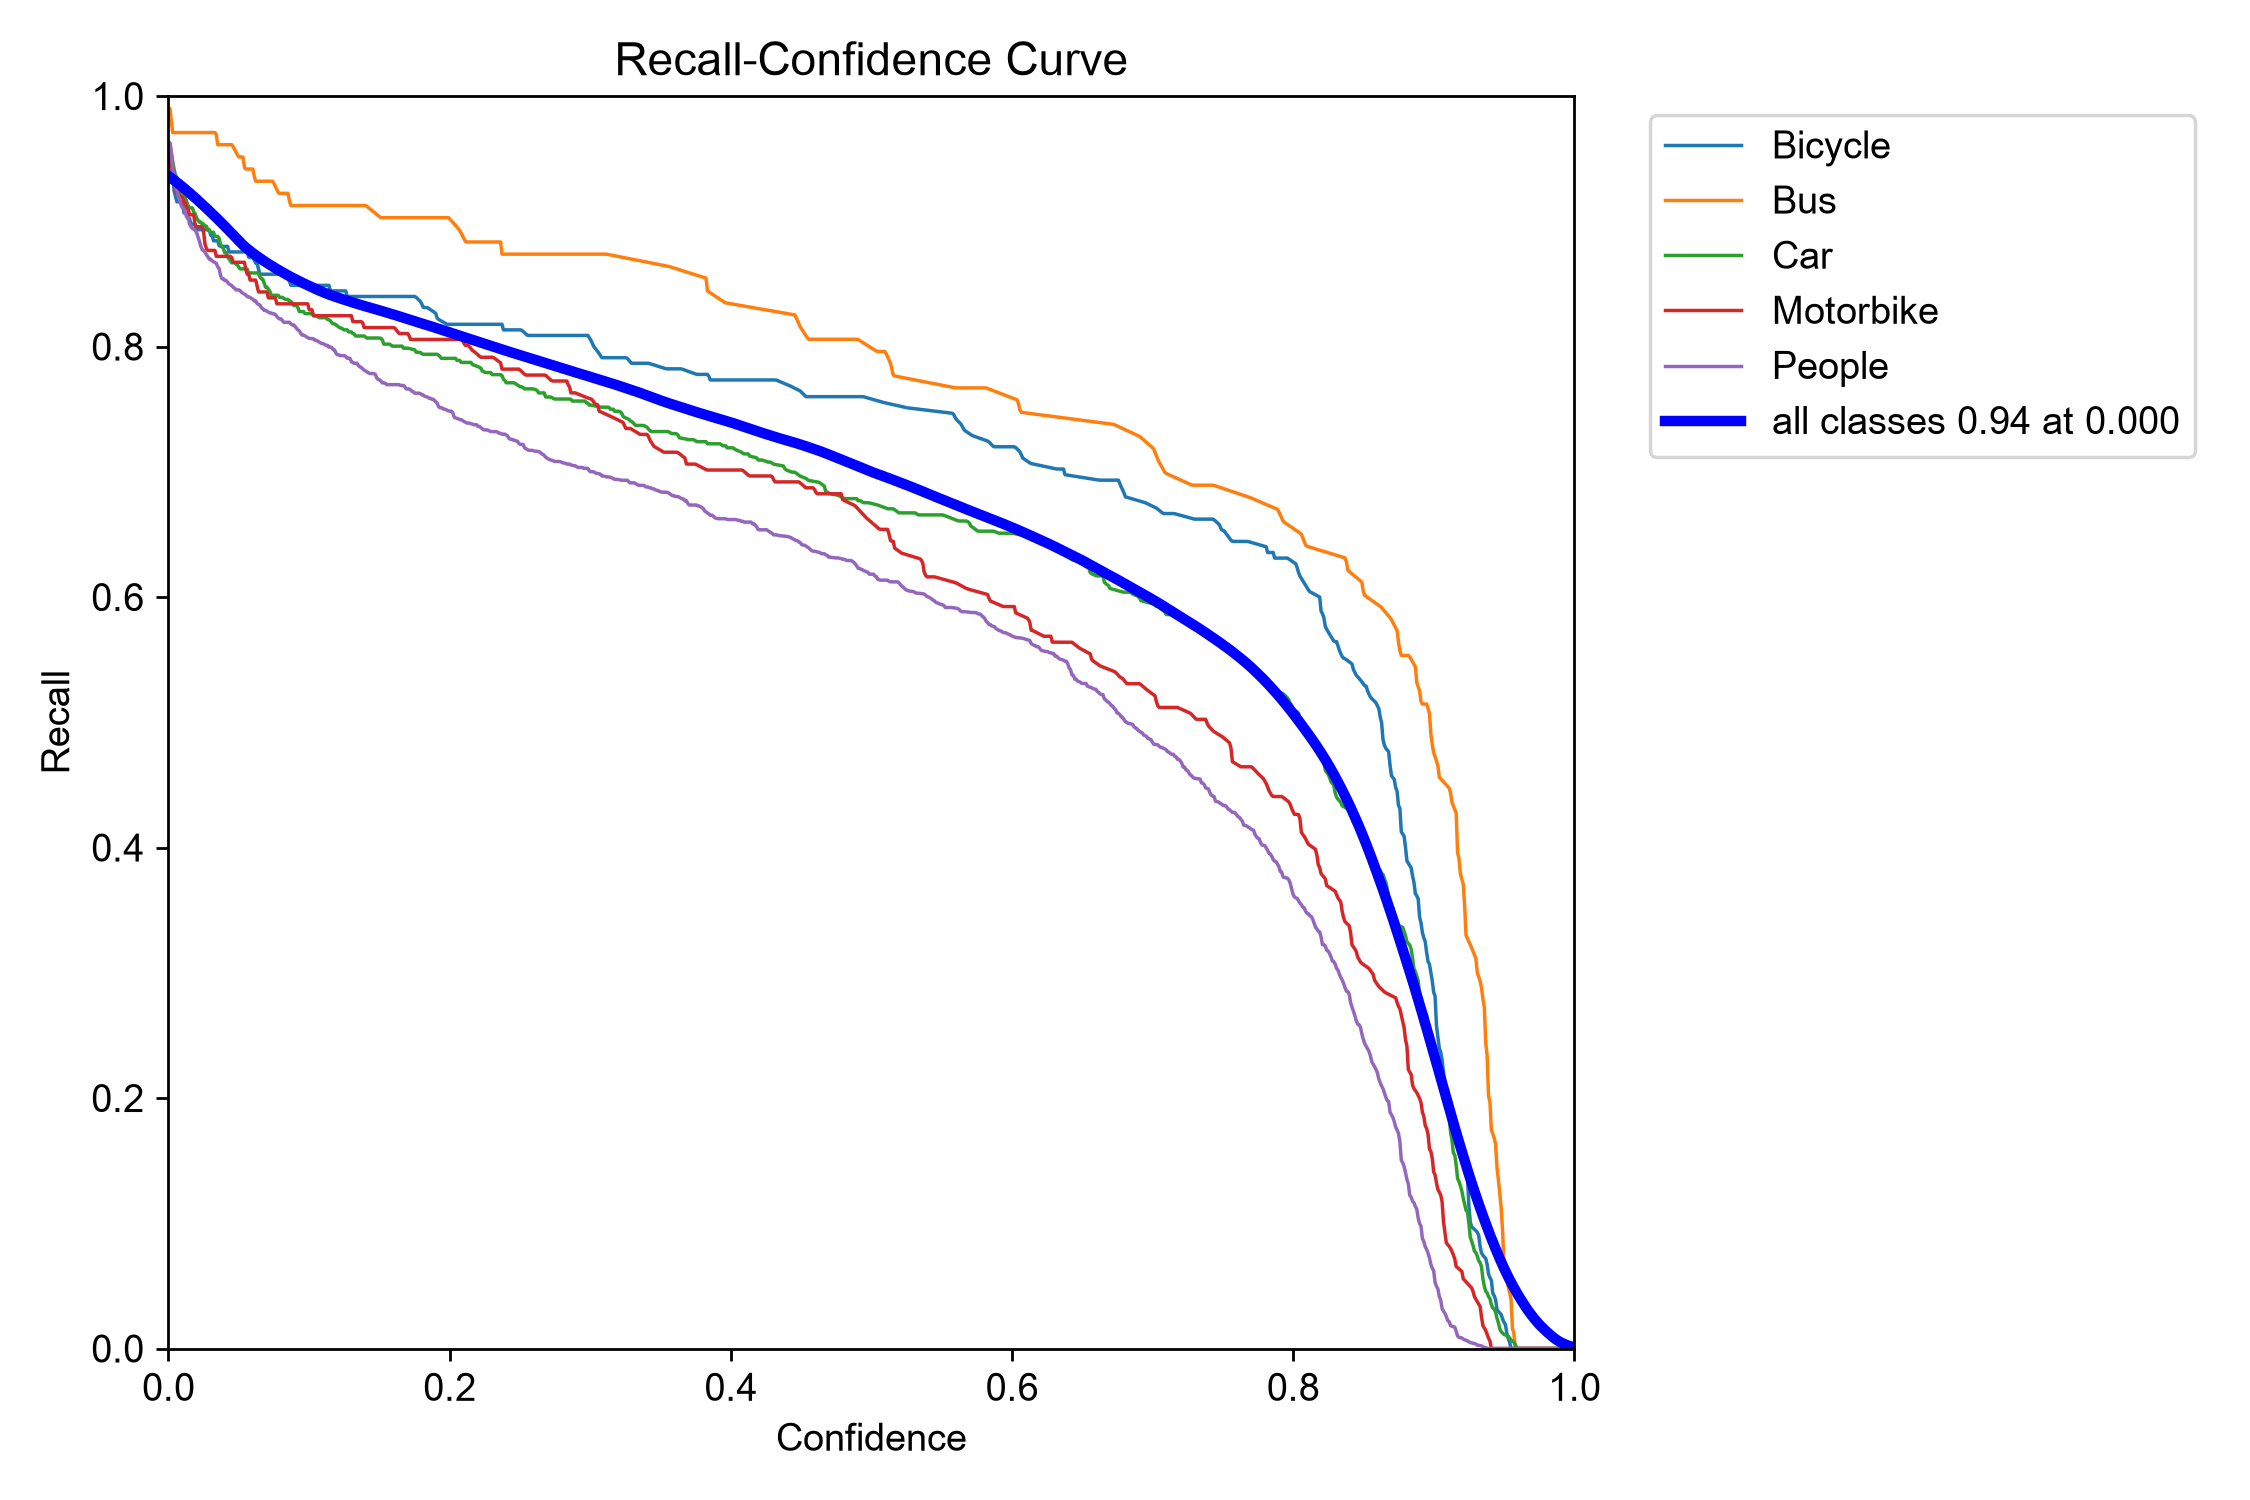
\includegraphics[width=\linewidth]{results/detection/night_traffic-2/BoxR_curve.png}\end{minipage}
\caption{Night-traffic confidence-dependent precision and recall.}
\label{fig:nt-pr}\end{figure}
\begin{figure}[t]\centering
\begin{minipage}{0.48\textwidth}\centering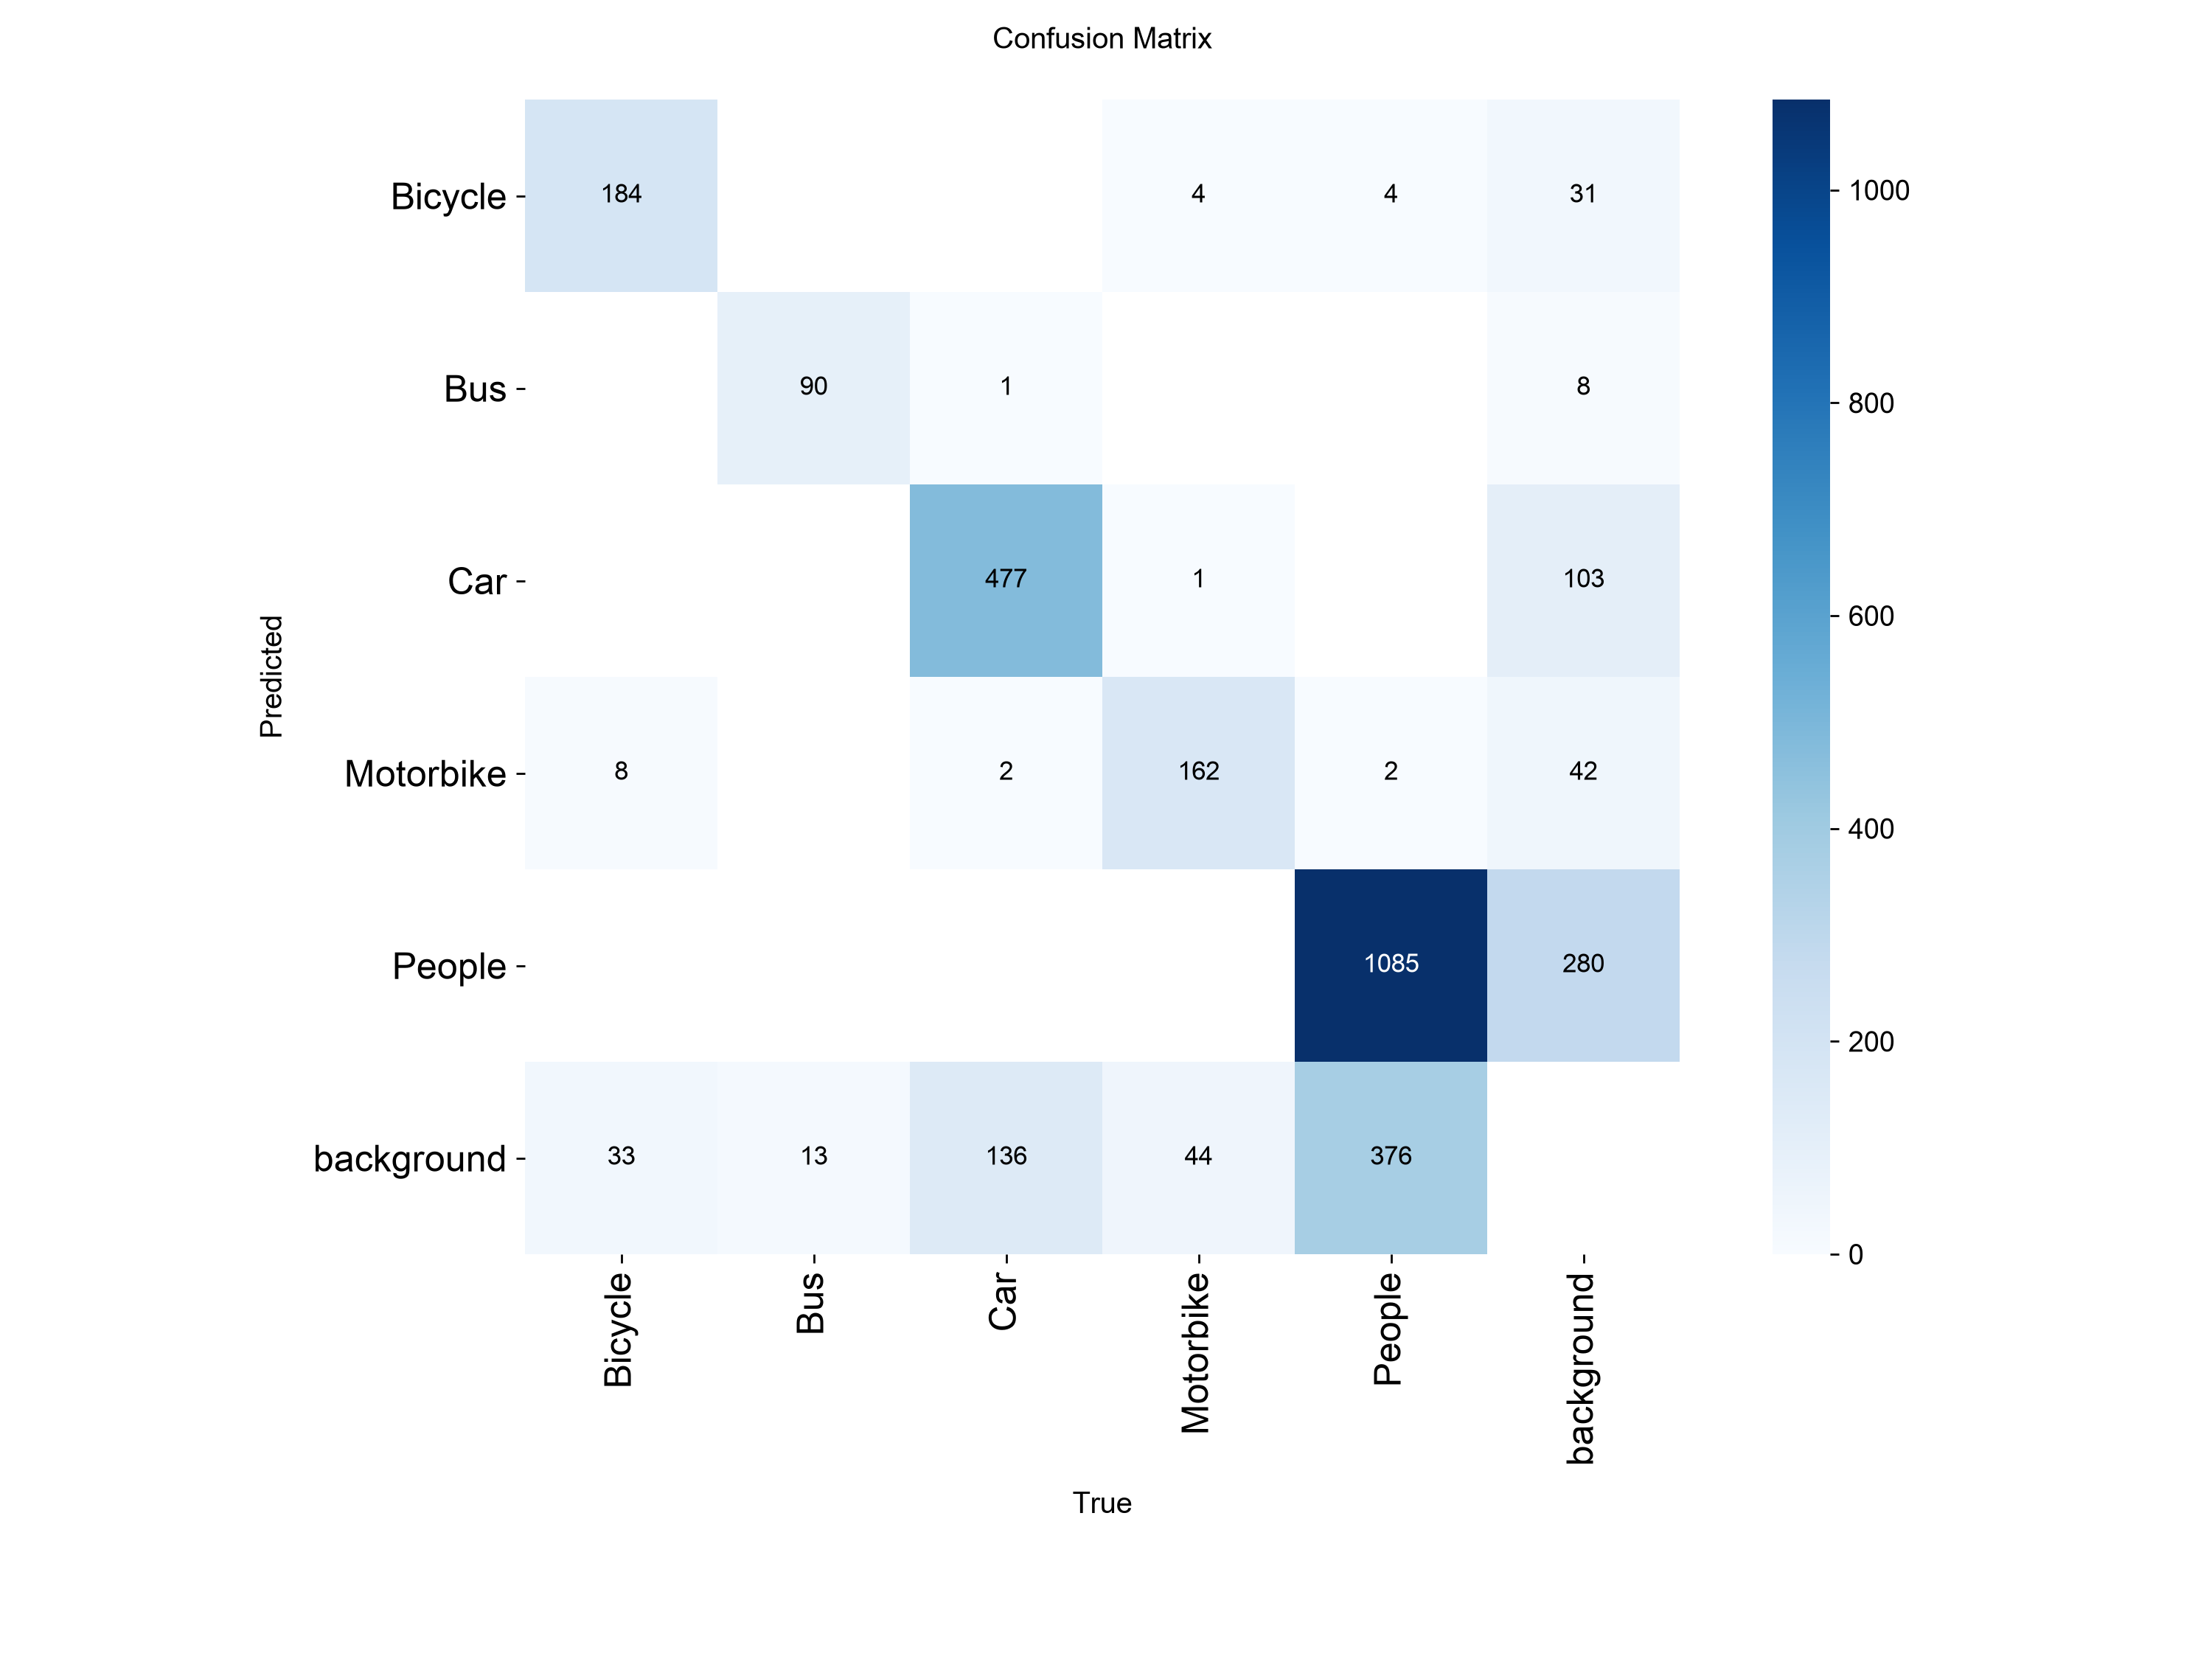
\includegraphics[width=\linewidth]{results/detection/night_traffic-2/confusion_matrix.png}\end{minipage}\hfill
\begin{minipage}{0.48\textwidth}\centering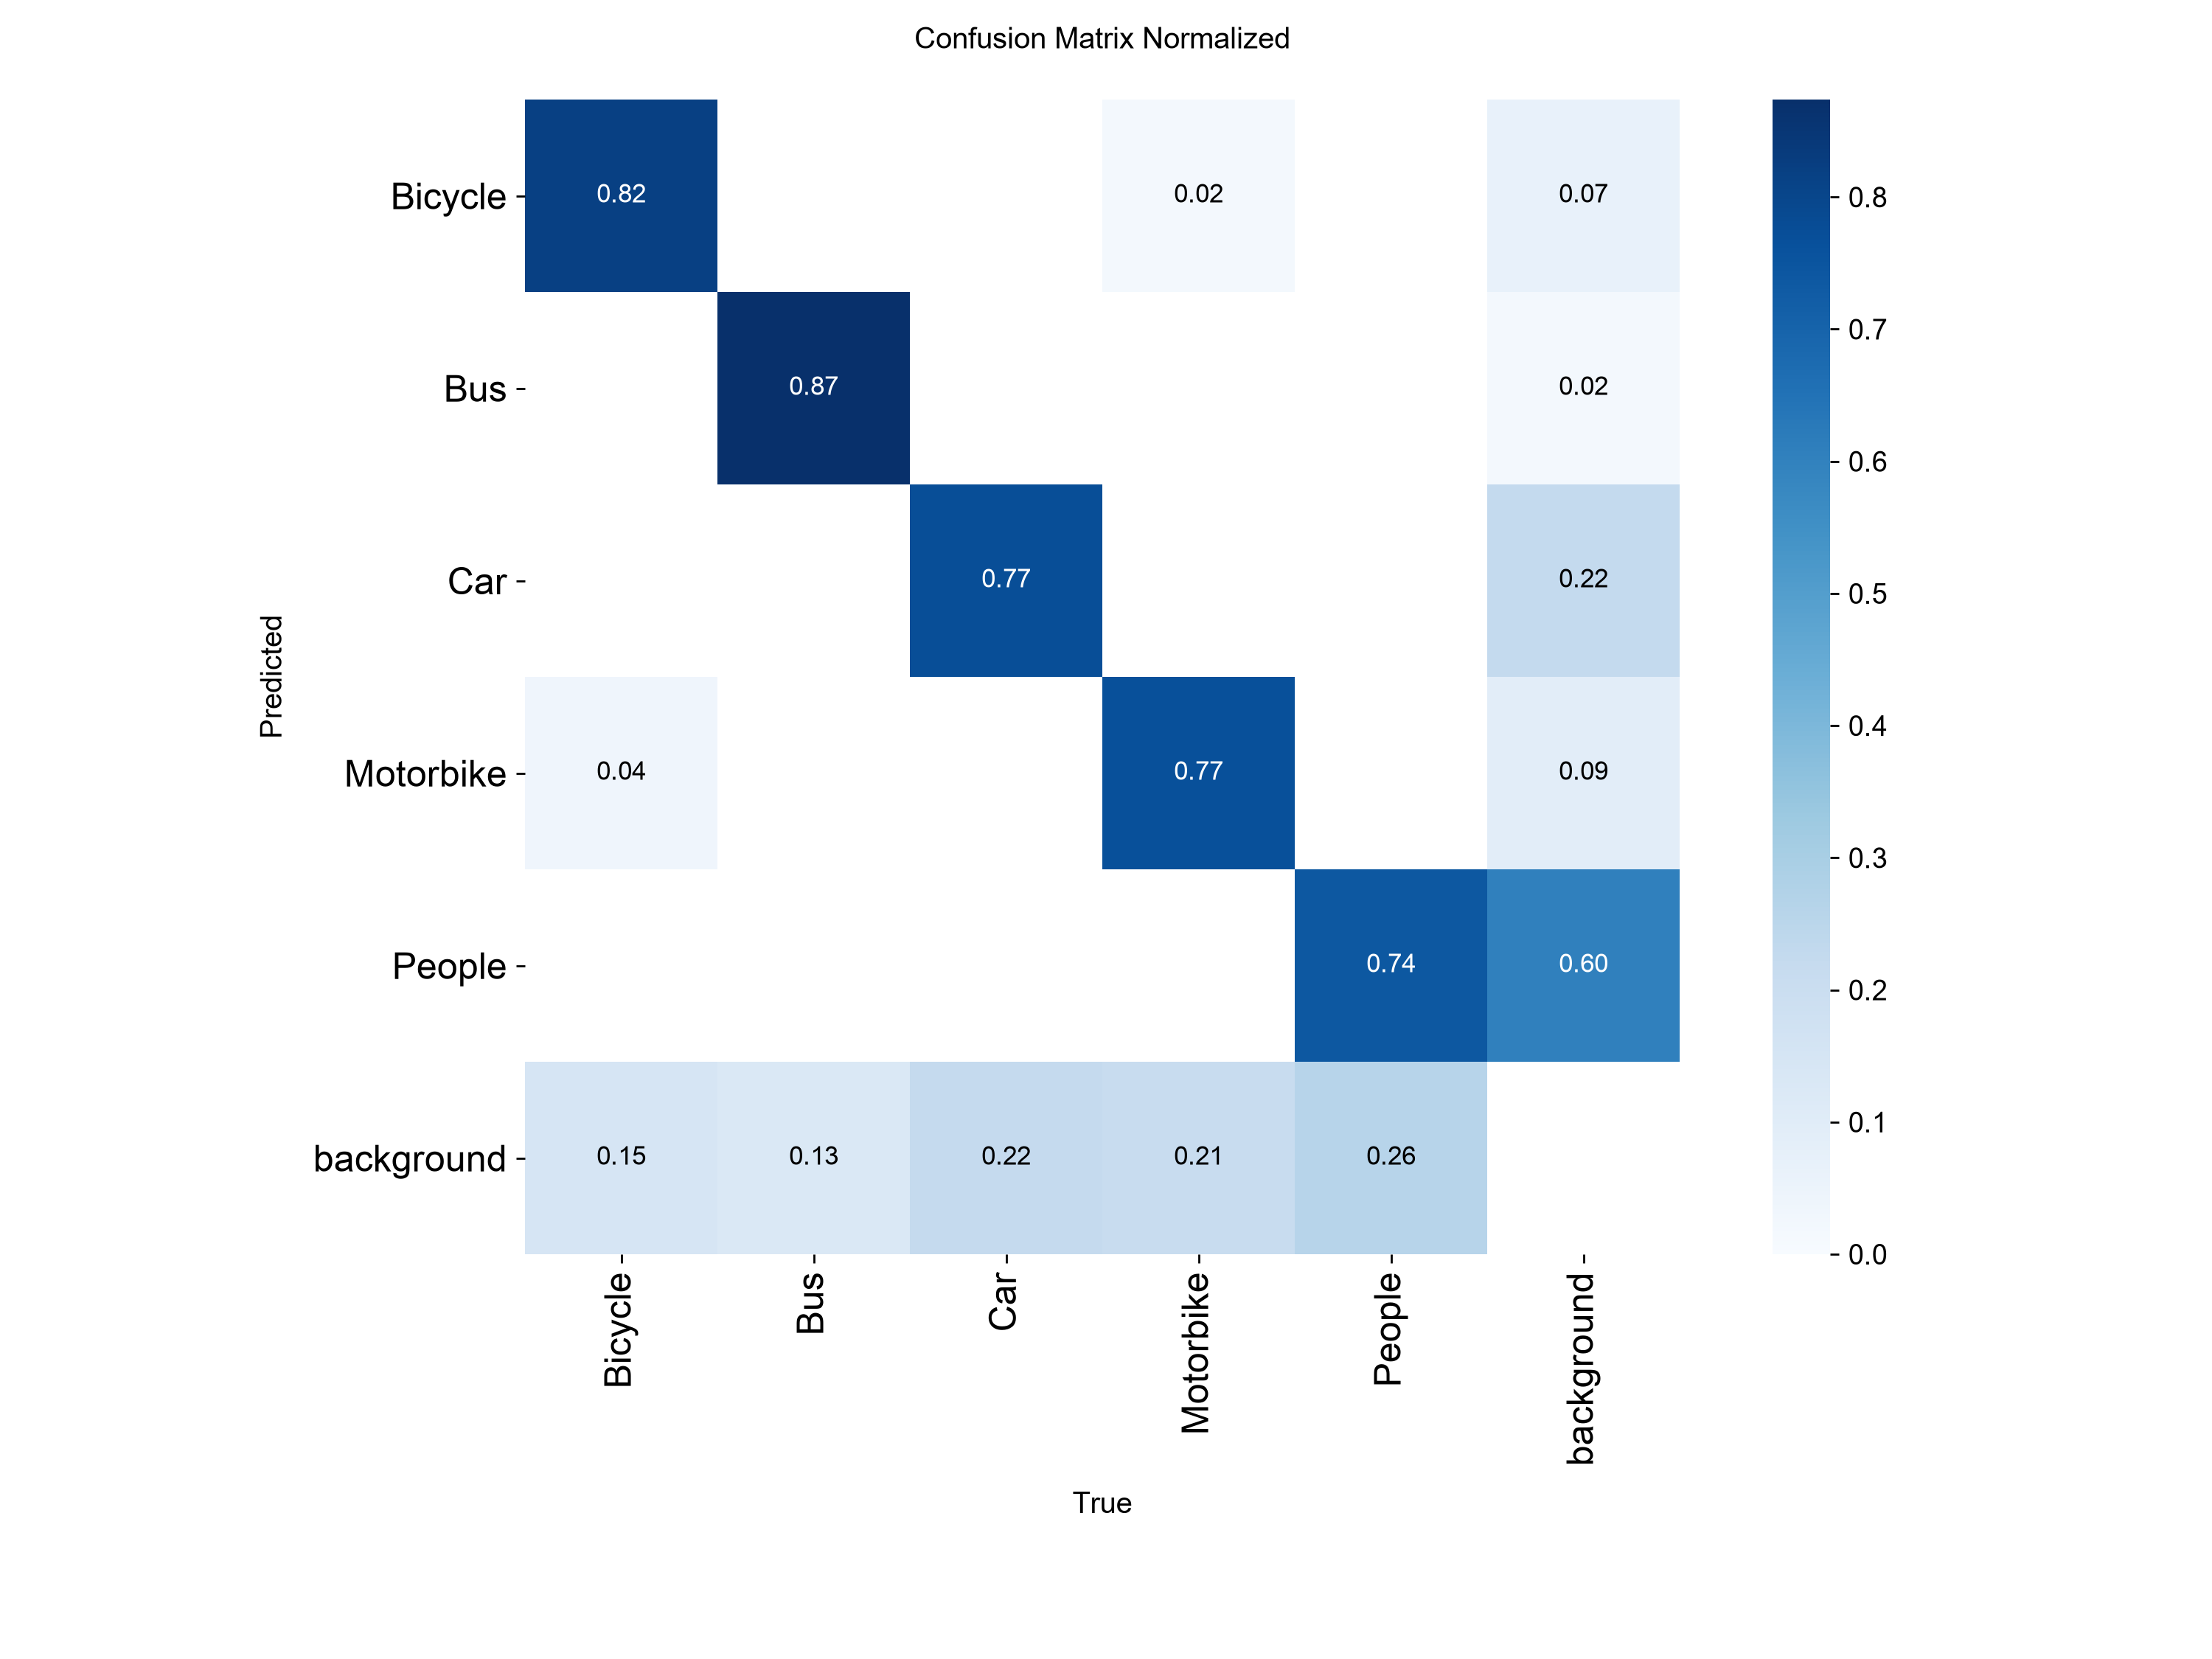
\includegraphics[width=\linewidth]{results/detection/night_traffic-2/confusion_matrix_normalized.png}\end{minipage}
\caption{Night-traffic raw and normalized validation confusion matrices.}
\label{fig:nt-conf}\end{figure}
\begin{figure}[t]\centering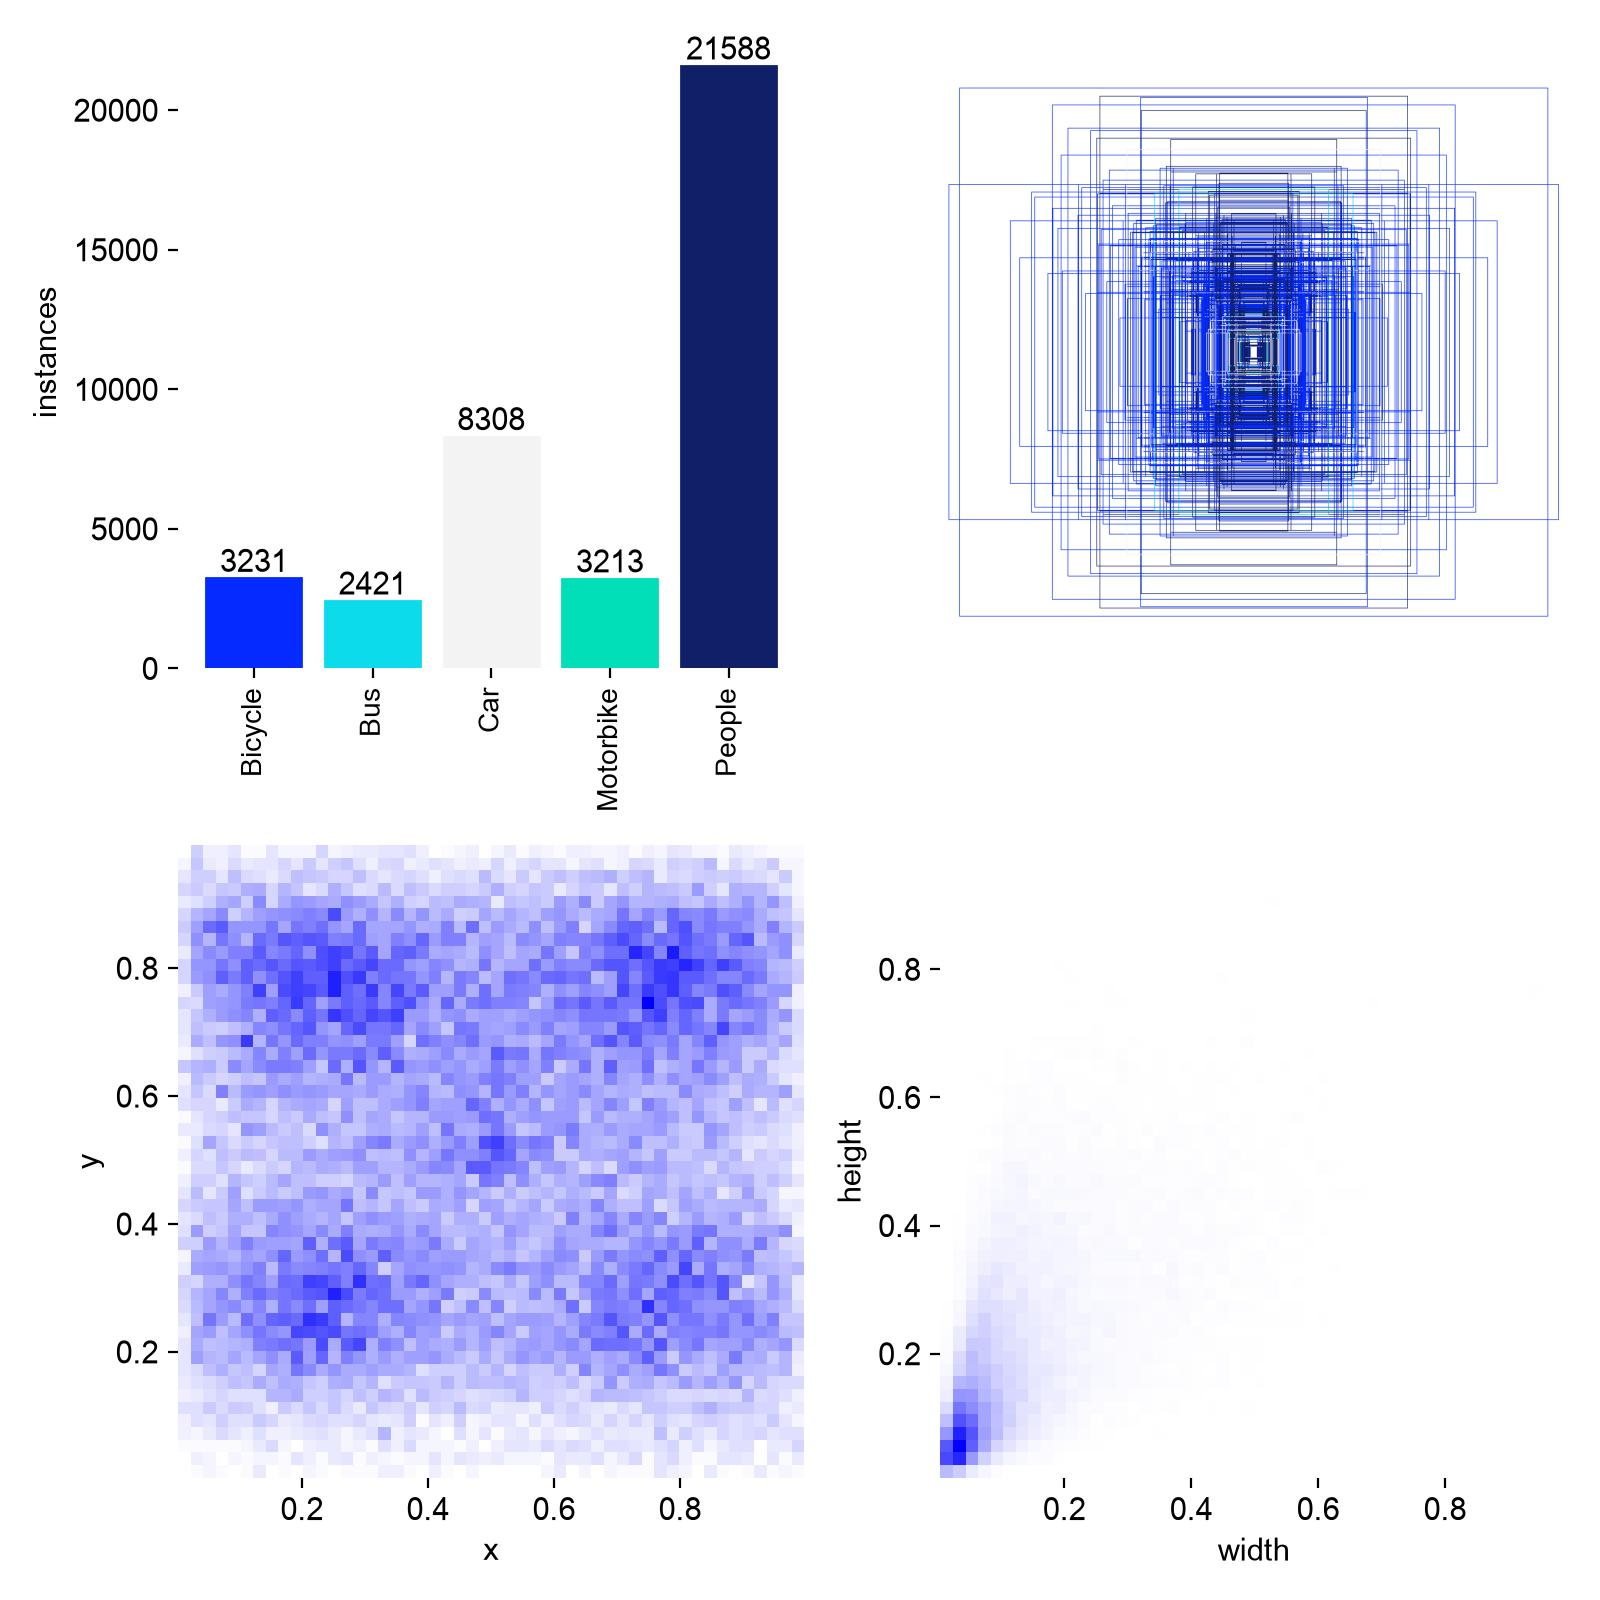
\includegraphics[width=0.78\textwidth]{results/detection/night_traffic-2/labels.jpg}
\caption{Night-traffic class labels and normalized box geometry.}
\label{fig:nt-labels}\end{figure}
The supplied comparison figure shows reported percentages from several papers, but common datasets, labels, splits, thresholds, and IoU conventions are not established. It is contextual evidence only. The proposed detector's displayed mAP@0.5 is 97.3\%; the chart also shows a prior value of 99.1\%, above this result.

\begin{figure}[t]\centering
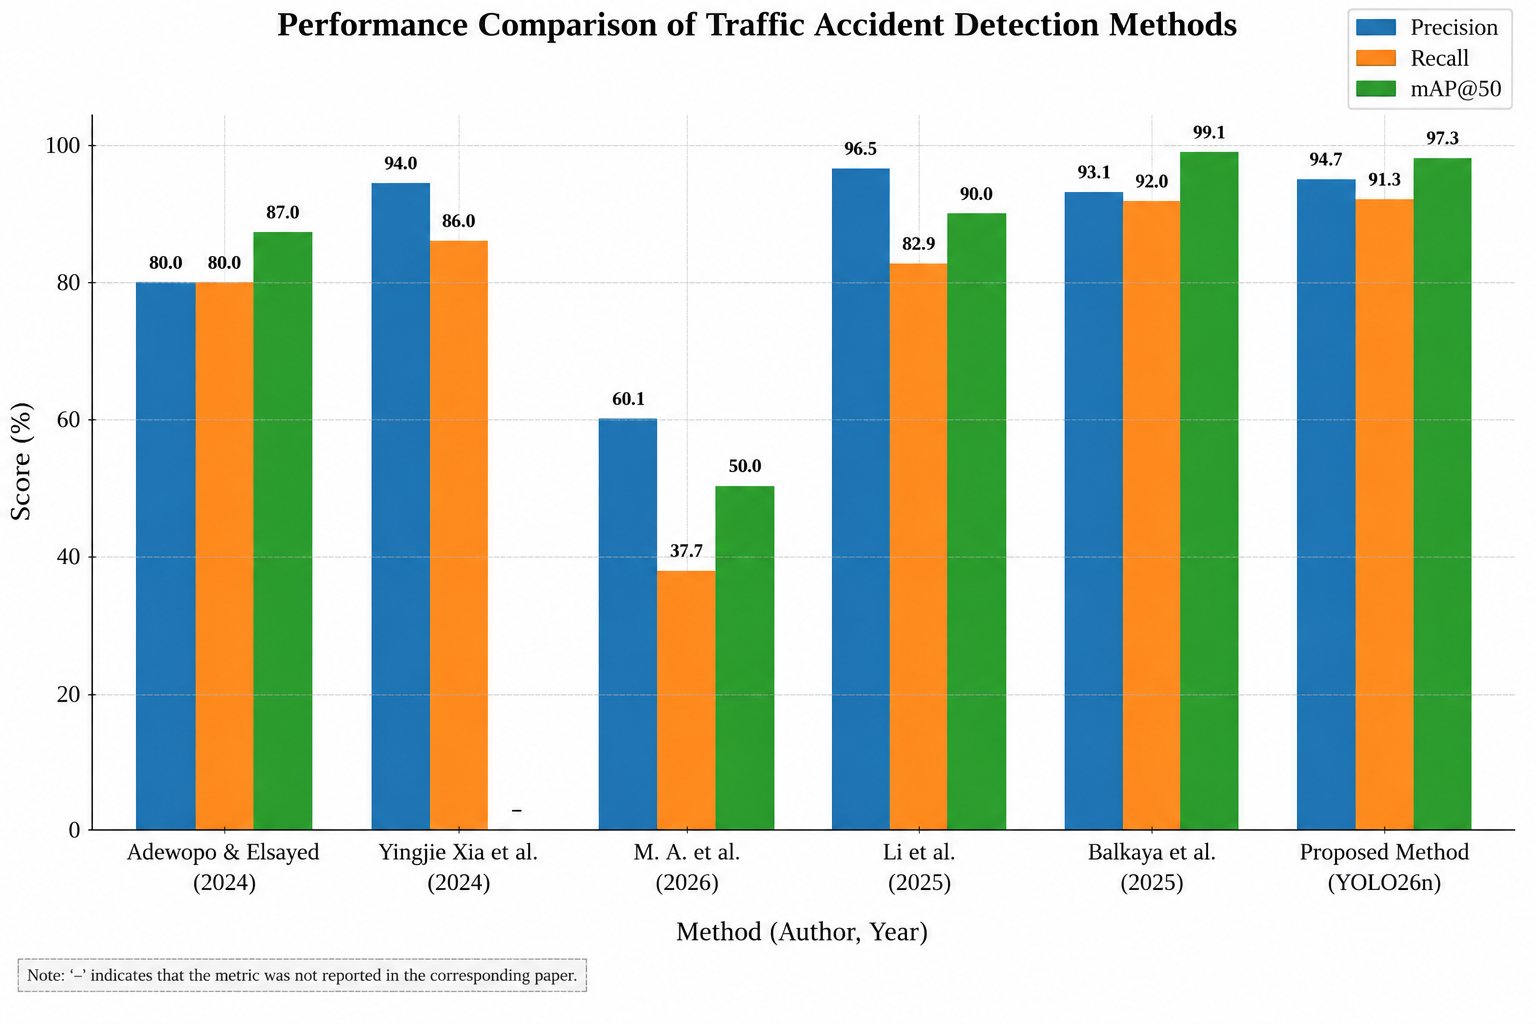
\includegraphics[width=0.92\textwidth]{results/project_comparison.png}
\caption{Comparison chart reproduced from the project presentation; it is not a controlled benchmark.}
\label{fig:comparison}\end{figure}
\section{Integrated Video Pipeline: Code-Level Analysis}
\subsection{Frame processing and model roles}


The severity class IDs map to MODERATE, NO\_ACCIDENT, and HIGH; the no-accident output is treated as a sentinel and filtered from the incident severity aggregation. If no usable severity vote remains, the displayed result becomes uncertain. This behavior is safer than equating every ambiguous crop to ``low,'' but confidence calibration, multi-crop aggregation behavior, and threshold selection are not established by the repository's evaluation artifacts.

\subsection{Temporal state behavior and latency}
The integration logic uses a three-frame confirmation threshold and an incident-gap value of 30 frames. A candidate becomes confirmed after repeated positive accident frames; an event remains in its aftermath state until a sufficient run of absent detections closes it. The standalone temporal-verification module similarly uses a state machine with candidate and active-aftermath states. It does not associate detections across frames by object identity or require the same accident class in every frame. Consequently, a sequence of unrelated accident-class boxes can satisfy the persistence count. Conversely, a single missed frame can reset a candidate in the simple verifier and suppress a real but intermittently occluded event.

The recorded integration example identifies the first detection at frame 59 and confirmation at frame 134, a 75-frame gap. The summary reports event duration as 75 frames (1.5 seconds), implying a nominal 50 frames per second for that calculation, although the input frame rate and precise frame accounting are not stored in the summary. This observed confirmation delay is far longer than three adjacent frame intervals, which indicates the event's positive detections were intermittent or the reported first-detection/confirmation definitions differ from the simple three-consecutive-frame rule. The source summary alone cannot resolve this discrepancy. A frame-level event trace with timestamps, per-model detections, and state transitions should be logged in future runs.

\subsection{Spatial and context checks are advisory in implementation}
The code defines a spatial-consistency check using IoU between the first and last boxes in the temporal buffer, with a lenient threshold of 0.10. It also computes a context status indicating whether road users are consistent with the accident class. However, the event-validation path assigns the verification decision as true even when these checks are false or context is insufficient; the checks therefore do not currently veto confirmation. They may enrich diagnostics, but should not be described as effective false-positive filters. The implementation should either connect them explicitly to state transitions or rename them as non-gating diagnostic evidence, then add tests for each branch.

\subsection{Media pipeline and output validation}

\subsection{Two saved demonstration records}
Two files in the integration-results directory contain effectively identical sample summaries: accident detected and verified; class car\_car\_accident; severity MODERATE at confidence 0.854; first detection frame 59; confirmation frame 134; event duration 75 frames (1.5 s); average accident confidence 0.842; maximum 0.923; 254 total frames; and listed detections of cars, motorbikes, and people. Processing rates are 10.12 and 10.68 FPS. These demonstrate a reproducible-looking prototype output for one short clip, but the duplicated summaries are not two independent test examples: their content and event measurements match, and likely represent repeated processing of the same sample. They provide no estimate of event sensitivity, false-alarm rate, or population-level reliability.

\section{Application, API, and Emergency-Workflow Audit}
\subsection{Service structure and endpoints}

The camera registry contains six hard-coded example locations across NH-44, NH-48, NH-16, and NH-65, each marked online. The analysis endpoint chooses a registered camera's coordinates for hospital lookup; an unknown camera ID falls back to the third demo camera. Thus, the location passed by the user is descriptive text and does not determine geospatial routing. A production system would need an authoritative camera registry, validation of coordinates and IDs, feed-health telemetry, and a clear rule for unknown cameras.

\subsection{Hospital service and location uncertainty}
The hospital service queries three public OpenStreetMap Overpass endpoints for named hospital features within a 30-km radius. It computes straight-line great-circle distance using the Haversine formula, sorts returned records, caches results in process memory, and has six near-camera fallback mappings. If the query and those fallback mappings fail, it returns Jagdamba Hospital with a 0.2-km distance regardless of the requested coordinates. This final unconditional fallback is geographically unsafe if the service is treated as live routing. It should instead return ``no verified facility found'' or an explicit low-confidence/unavailable state.

The API returns the nearest named feature by straight-line distance. It does not establish facility capability, emergency department status, current availability, capacity, travel time, ambulance routing, or data freshness. Overpass availability and rate limits can delay the synchronous analysis request. Cache state is process-local, so it is not shared across server workers and disappears on restart. The service should identify the lookup timestamp and source, distinguish live results from static fallbacks, apply bounded timeouts, and expose alternatives and uncertainty.

\subsection{Alert state, persistence, and access controls}
Alerts are stored in a module-level in-memory Python list. Creation, acknowledgement, dispatch, and reset mutate that list. Restarting the server loses the state; multiple worker processes do not share the same records; concurrent updates have no transactional protection. Dispatch time and ETA are demo fields: ETA is calculated from straight-line distance as distance times 2.5, with a two-minute floor, rather than a road-routing service. The server's CORS configuration allows every origin while credentials are enabled, and the inspected endpoints do not apply authentication or authorization. These are acceptable constraints for a local classroom prototype only after it is clearly isolated; they are not a safe basis for a public emergency service.

The dashboard's acknowledgment endpoint records a hospital name inferred from the selected hospital data, not a verified authenticated user identity. Dispatch endpoints similarly set a status and timestamp from a request without an actual dispatch integration. These semantics should be called simulated acknowledgment/dispatch in the interface and paper. A future deployment requires identity, access policies, audit trails, idempotent operations, persistent storage, event signing, retry rules, rate limits, abuse protection, and an explicit distinction between an operator's decision and an automated recommendation.

\subsection{Privacy, cybersecurity, and operational safety}
Video upload is saved using a filename containing the original user-supplied filename. The implementation should sanitize path components, constrain file size and accepted codecs, use random opaque names, and define deletion/retention behavior. The inspected upload path copies content to a static uploads directory; public static serving of uploaded or derived media should be assessed carefully for sensitive footage. The server binds to all network interfaces when started, so network exposure depends on host firewall and environment configuration. These observations are code-review findings, not evidence that the application was publicly deployed or exploited.

No real emergency dispatch should be triggered solely by a model result. A safe workflow keeps a trained human reviewer in the loop, shows the source clip and uncertainty, flags camera failure, and records review and correction. Before any pilot, use offline replay and silent-mode evaluation, then a supervised advisory phase with an authorized partner. The alert system needs documented privacy purpose, data minimization, access controls, encryption, retention schedule, incident-response procedures, and a security review.

\section{Project Scope, Requirements, and Design Goals}
The project objective is to support CCTV operators by identifying candidate road accidents, estimating visible severity, and organizing information for human response. The intended workflow begins with a video source and ends with an operator-facing incident record. Its scientific and operational boundaries are important: the models process images and video; they do not independently establish injuries, decide clinical triage, or dispatch emergency vehicles. A human reviewer remains the safe final decision-maker.

The system has functional requirements and quality requirements. Functional requirements include reading a clip, decoding frames, running one or more detectors, filtering outputs, verifying candidate events over time, assigning a visual severity category, recording camera and location metadata, looking up nearby facilities, and presenting a dashboard record. Quality requirements include timely processing, traceable predictions, predictable failures, privacy protection, secure access, and accurate representation of uncertainty. The project demonstrates many functional paths, but does not supply measurements for availability, failure recovery, alert delivery, security, or response outcomes.

The principal outputs are an event flag, accident interaction type, confidence, severity category, frame interval, camera metadata, video artifact, and nearby facility list. An operational incident should also identify its source camera and time, retain uncertainty about its location, maintain a unique incident identifier, and record every state transition. The current prototype's summary and dashboard provide a useful basis for this record, but the underlying state is not durable and the camera registry is demonstrative.

The target users are highway-monitoring staff and facility-side viewers. They need a short event clip with nearby frames, model labels, confidence, severity uncertainty, camera status, and actions for acknowledgement or rejection. Interface language should clearly distinguish model estimates and demo workflow statuses from verified dispatch. This is especially important because a false positive can create needless work while a false negative can delay human awareness. User-interface evaluation and operator workload studies have not been performed.

The system should fail visibly and safely. If an input cannot be decoded, the camera should be marked unavailable. If temporal evidence is insufficient, the event should remain a candidate. If severity is uncertain, the interface should preserve an uncertain label rather than silently converting it to low severity. If location cannot be verified, the service should report unavailable, not substitute an unrelated facility. These behaviors are design requirements for future versions; this report distinguishes them from code behavior observed in the prototype.

\section{Data Inventory and Label Interpretation}
In addition to the two primary accident and severity datasets, the repository contains a night-traffic dataset with 8,292 images split into 7,033 training, 840 validation, and 419 test images; it uses Bicycle, Bus, Car, Motorbike, and People classes. A broader night-vision collection contains 12,489 images split into 10,288/1,465/736 and twelve classes, including boat, bottle, cat, chair, cup, dog, and table. That collection is a general object-detection resource and should not be presented as an accident dataset. Dataset counts and label-file checks establish structural consistency only.

The accident ontology combines event-like labels and object-like labels. Seven labels encode interactions (bike--bike, bike--object, bike--person, car--bike, car--car, car--object, and car--person), whereas bike, car, and person denote ordinary objects. Annotation rules should explain whether an interaction label requires visible contact, a post-impact configuration, or simply nearby objects. They should also explain near misses, damaged stationary vehicles, occlusion, ambiguous evidence, multiple simultaneous events, and bounding-box boundaries. The saved repository does not provide a complete annotation guide.

Severity classes are moderate-accident, no-accident, and severe-accident. The severity inventory reports 4,452 images and 9,408 object annotations. Their proportions are 19.75\%, 50.67\%, and 29.58\%. The distinction between image counts and annotation counts matters because one image may contain multiple boxes. The labels appear in an object-detection format, while the system consumes a cropped region to produce a single incident-level category. Documentation should specify how crop labels are produced, what happens when several boxes are present, and how a frame prediction becomes an incident prediction.

Split construction is a central validity issue for video-derived datasets. If adjacent frames from a source clip are randomly distributed, near-identical scenes can occur in both training and validation sets. This inflates apparent generalization. The current counts do not establish whether source clips or cameras were grouped. A future manifest should retain source-video identifiers, camera identity, recording date where permissible, and hashes for exact and near-duplicate detection. Test data should remain untouched during threshold selection.

The data-inspection scripts report matching image and label file counts in the reviewed split directories. For severity, they identify seven very large boxes while reporting no missing files, empty labels, invalid class IDs, invalid formats, or out-of-bounds boxes in the particular inspection. Those checks are useful for catching file-structure errors, but cannot verify semantic label truth, appropriateness of class assignment, or agreement between annotators. A randomly sampled visual audit is still required.

\section{Detailed Model Results and Interpretation}
The three saved YOLO26n runs have distinct label spaces and evaluation conditions. The accident model detects a mixture of interactions and ordinary objects. The severity run has three accident-state labels. The night-traffic detector recognizes road users in its configured dataset; it is not an accident-event model. The broad night-vision dataset has no separate model metrics included here. These scopes must remain distinct when reading aggregate values.

For accident detection, the training CSV contains 100 epoch rows, and the results folder contains best and last checkpoints, arguments, curves, confusion matrices, and validation examples. The recorded final row gives precision 0.94701, recall 0.91308, mAP@0.5 0.97321, and mAP@0.5:0.95 0.84124. The highest logged precision is 0.95137 at epoch 99; highest recall is 0.94558 at epoch 81; highest mAP@0.5 is 0.97347 at epoch 97; and the mAP@0.5:0.95 maximum is the final 0.84124 at epoch 100. These are different checkpoint epochs and should not be combined into a synthetic best row.

The PR plot displays nine AP@0.5 values: bike 0.971, bike--bike 0.969, bike--person 0.995, car 0.989, car--bike 0.940, car--car 0.985, car--object 0.968, car--person 0.995, and person 0.947. Their mean is close to the reported overall value. Bike--object does not appear in the legend, so the metric cannot support that class. The confusion matrices include background accounting for missed or unmatched detections; they are not simple classification accuracy matrices. The normalized confusion plot emphasizes proportions, while the raw matrix preserves count information.

The severity run has a meaningful validation-to-test distinction. Its best validation summary gives approximately 80.20\% precision, 75.20\% recall, 82.52\% mAP@0.5, and 60.62\% mAP@0.5:0.95, whereas its independent saved test summary gives 79.74\%, 71.81\%, 80.45\%, and 55.47\%. The per-class test values show AP@0.5 of 81.39\% for moderate, 81.43\% for no-accident, and 78.54\% for severe. Test recall is 74.65\%, 70.30\%, and 70.50\%, respectively. These estimates have no reported confidence intervals. As the classes imply an order, future analysis should include ordinal errors and a confusion matrix.

The severity test timing is 2.7 ms preprocessing, 8.2 ms inference, and 0.2 ms postprocessing per image. The combined 11.1 ms suggests an idealized serial rate around 90 images per second, but excludes video decoding, crop preparation, other model calls, temporal logic, file output, and dashboard/network time. It should not be interpreted as integrated throughput. The integrated demonstration runs at about 10 frames per second, which is a distinct measurement under incompletely recorded hardware conditions.

The night-traffic model's final validation metrics are precision 83.960\%, recall 77.684\%, mAP@0.5 85.307\%, and mAP@0.5:0.95 57.371\%. Its metric-specific best values are 87.343\% precision at epoch 89, 77.684\% recall at epoch 100, 85.450\% mAP@0.5 at epoch 98, and 57.442\% mAP@0.5:0.95 at epoch 99. Its stricter-mAP gap is 27.936 points. No class-by-condition metadata or matched daylight comparison is available, so the result only characterizes the configured road-user validation task. The integration code classifies a frame as dark when mean grayscale luminance is below 100. It converts the frame to Lab color space, applies CLAHE to the L channel, and sends the enhanced frame to the night-traffic detector. This fixed heuristic may misclassify tunnels, twilight, headlights, or locally shadowed scenes. No paired ablation establishes whether the transform improves event recall or calibration.

Across all models, validation curves and confusion matrices are useful development diagnostics, not evidence of deployment readiness. The absence of confidence intervals, repeated seeds, external-camera evaluation, and video-event matching should be visible alongside reported scores. A high precision estimate can still lead to many false alerts when event prevalence is low; an operating point must be chosen against measured camera-hour prevalence and the cost of missed incidents.

\section{Architecture and Data Flow in More Detail}
The acquisition layer reads a local video or submitted sample, decodes frames, and prepares image arrays for inference. The configured training size is 640 pixels, while the application path includes frame decoding and image crops. Any production camera source would require reconnect logic, frame timestamps, dropped-frame monitoring, and a camera registry tied to reliable location metadata. The current demonstration does not document production stream ingestion.

The inference layer uses a night-traffic detector for road-user context, an accident detector for interaction candidates, and a severity detector for a padded crop. Ordinary object detections from the accident model do not alone trigger the incident flag. The selected severity class IDs map to MODERATE, NO\_ACCIDENT, and HIGH; the no-accident class is a sentinel, and absence of a usable severity vote is treated as uncertain. The project report does not provide the crop aggregation rule or calibration data.

The temporal layer maintains candidate and aftermath states. Integration logic confirms after three positive frames and uses a 30-frame gap value to keep an event active. The standalone verifier does not track object identity or require the same accident class for every positive. Therefore, unrelated detections may satisfy persistence, while a single missed positive can reset a simple candidate. The spatial-consistency calculation uses IoU between first and last boxes with a lenient threshold of 0.10. The code also calculates context consistency. However, event validation sets the decision to true even when these checks fail or context is insufficient. These checks provide diagnostics and currently do not gate confirmation.

The application layer wraps video processing in a FastAPI service. Endpoints cover cameras, sample videos, analysis, alert listing and creation, acknowledgement, dispatch status, and demo reset. Analysis synchronously runs inference, parses a plain-text summary, and returns structured fields and an output video location. Long clips may hold a request open because no queue or progress channel is evident. A production design should submit bounded background jobs and return a job identifier, status, and progress.

The location service queries public OpenStreetMap Overpass endpoints for hospital-like features within 30 km, computes straight-line Haversine distances, sorts results, and caches results in process memory. Six camera-specific fallbacks exist. If those fail, an unconditional fallback returns Jagdamba Hospital at 0.2 km regardless of coordinates. Straight-line distance does not establish route time, facility capability, emergency department status, capacity, or current availability. The result should be treated as a demo lookup only.

The dashboard and alert service store state in an in-memory Python list. Restarting loses alerts; multiple worker processes do not share state; simultaneous updates are not transactional. There is no authentication or authorization on inspected endpoints, while CORS permits every origin with credentials. Acknowledgement and dispatch are simulated status changes. Public exposure would require durable storage, identity and role checks, audit records, restricted CORS, idempotent operations, rate limiting, upload validation, media retention rules, and security review.

\section{Recommended Project Work Plan}
The first priority is data and label provenance. Resolve YAML paths and historical dataset roots, record hashes and licenses, retain a split manifest, check exact and near duplicates, and group samples by source clip and camera. Publish a label dictionary and annotation guide for every task. Review a representative sample with multiple annotators, report agreement, and preserve uncertain labels rather than forcing ambiguous scenes into a severity category.

The second priority is model evaluation. Freeze a camera-disjoint and source-video-disjoint test set. Re-run the accident and severity models with fixed configurations and multiple random seeds. Report per-class support with every metric, confidence intervals bootstrapped over clips, confusion matrices, and threshold curves. For the rare accident classes, collect and verify substantially more examples. Do not claim that rebalancing, augmentation, or class weighting improves performance until an identical held-out protocol shows an improvement.

The third priority is event-level testing. Annotate onset, impact interval, end time, event type, camera, visibility, and severity rubric. Compare single-frame thresholding, the current temporal filter, a track-aware rule, and any learned temporal approach using the same detector checkpoint. Record false alarms per camera-hour, event recall, confirmation delay, duplicate alerts, missed events, and onset error. Include one- and two-frame occlusions, overlapping incidents, drifting boxes, dropped frames, and hard negative scenes.

The fourth priority is integration reliability. Build replay tests for decoding, inference, event state, severity aggregation, hospital lookup, output-video validity, and dashboard state transitions. Simulate Overpass timeouts, empty facility results, malformed summaries, server restart, concurrent acknowledgement, and network interruption. Record source timestamps and per-stage runtimes. Replace the unconditional facility fallback with an explicit unavailable result and report source, timestamp, alternatives, and location uncertainty.

The final priority is supervised operational evaluation. Begin with offline replay; proceed to silent recording without changing response; then run a supervised advisory test with an authorized highway or emergency-response partner. Define stop conditions for false-alert burden, missed events, stale camera information, incorrect facility lookup, and service outages. No research test should trigger real emergency dispatch solely because of model output.

\section{Report Scope and Evidence Conventions}
Project-specific statements in this report are tied to supplied slides, source code, saved run artifacts, or demonstration summaries. A saved metric means the value exists in a run CSV or summary; it does not mean an independent reproduction. A code-review observation describes the implementation path inspected; it does not establish that the service was deployed publicly. Proposed requirements and evaluation actions are recommendations rather than features already implemented.

The local figure paths reproduce files from the uploaded results hierarchy. Accident and severity figures document model curves, confusion matrices, label distributions, training batches, and validation examples. The night-traffic run contributes its own saved validation figures. The comparison chart is included as presented. The source repository remains the authority for model checkpoints; this report contains no model weights.
\section{Limitations and Threats to Validity}
\subsection{Source-material limitations}
This analysis uses the supplied capstone slides and the accessible project repository at the provided path. The repository includes three YOLO26n run folders with checkpoints, settings, epoch logs, plots, and validation examples; the severity run also includes a text summary with test metrics. The saved checkpoints were not re-evaluated here, so logged values are not independent reproductions. Training arguments retain a historical absolute data path, and the reviewed YAML relative paths appear inconsistent with the current split layout; the exact data files consumed during original training therefore need confirmation. The backend and inference code were inspected, but no production service or live dispatch integration was available for evaluation. Claims are limited to code and artifacts in the repository.

The repository contains some split counts and the severity training summary names an NVIDIA GeForce RTX 3050 Laptop GPU, but a complete manifest, annotation guidelines, complete hardware/software environment, event-level labels, and fresh independent evaluation are absent. The logged scores cannot be independently reproduced from the current path without resolving dataset-path provenance. Names in the comparison chart are abbreviated, and cited values are not verified as a matched benchmark. These constraints should accompany any submission or demonstration of reported performance.

\subsection{Construct validity}
If frame labels denote collision-related objects rather than event occurrence, detector mAP may measure object localization but not incident detection. Likewise, visual severity categories may not correspond to actual injury severity. The chosen metrics may therefore only partially measure the intended constructs. A label dictionary and annotation protocol are needed to establish this mapping.

\subsection{Internal validity}
Without split construction and source-video grouping, leakage through adjacent frames cannot be ruled out. Without a documented operating threshold and checkpoint selection rule, metric selection bias cannot be assessed. The validation values are reported as given, but the evidence is insufficient to rule out these threats.

\subsection{External validity}
Generalization across camera installations, geography, traffic patterns, weather, lighting, vehicle types, and incident composition is unknown. A public image dataset may not represent live highway CCTV. A detector can learn scene-specific correlations such as road markings, camera geometry, or compression characteristics. Cross-camera testing is a minimum step toward external validity.

\subsection{Statistical validity}
No confidence intervals or repeated-run variability are provided. Aggregate precision, recall, and mAP should be accompanied by uncertainty estimates, especially for small or imbalanced evaluation subsets. Bootstrap resampling should be performed at the clip or event level rather than frame level to preserve temporal dependence.

\subsection{System validity}
Dashboard and alert features do not by themselves prove integration with real emergency services. No API contract, network reliability measurement, dispatch confirmation, or end-to-end timing result is available. A lab prototype can demonstrate a user flow, but a live emergency service demands stronger verification and operational governance.

\section{Conclusion}
This paper evaluated the saved accident-detection and severity runs and reviewed their integration into a monitoring prototype. The accident detector achieved final logged validation precision/recall/mAP@0.5/mAP@0.5:0.95 of 94.701/91.308/97.321/84.124\%. Severity validation values were 76.174/77.897/82.157/60.530\%; the separate test summary gives 79.74\% precision, 71.81\% recall, 80.45\% mAP@0.5, and 55.47\% mAP@0.5:0.95. Results remain repository-reported, with strong class imbalance and incomplete source-video and event-level evidence.

The integrated video demonstration shows the intended user flow, but does not establish population-level reliability or faster emergency response. Code review identified non-gating spatial/context checks, a fixed-facility fallback, and volatile unauthenticated alert state. The system should therefore be treated as a human-supervised prototype. The next steps are source-video-disjoint evaluation, event-level temporal metrics, severity rubric validation, and a secure, partner-reviewed alert workflow.\appendix
\section{Supplementary Saved Run Figures}
\section{Accident Detection Training and Validation Previews}
\begin{figure}[t]\centering
\begin{minipage}{0.32\textwidth}\centering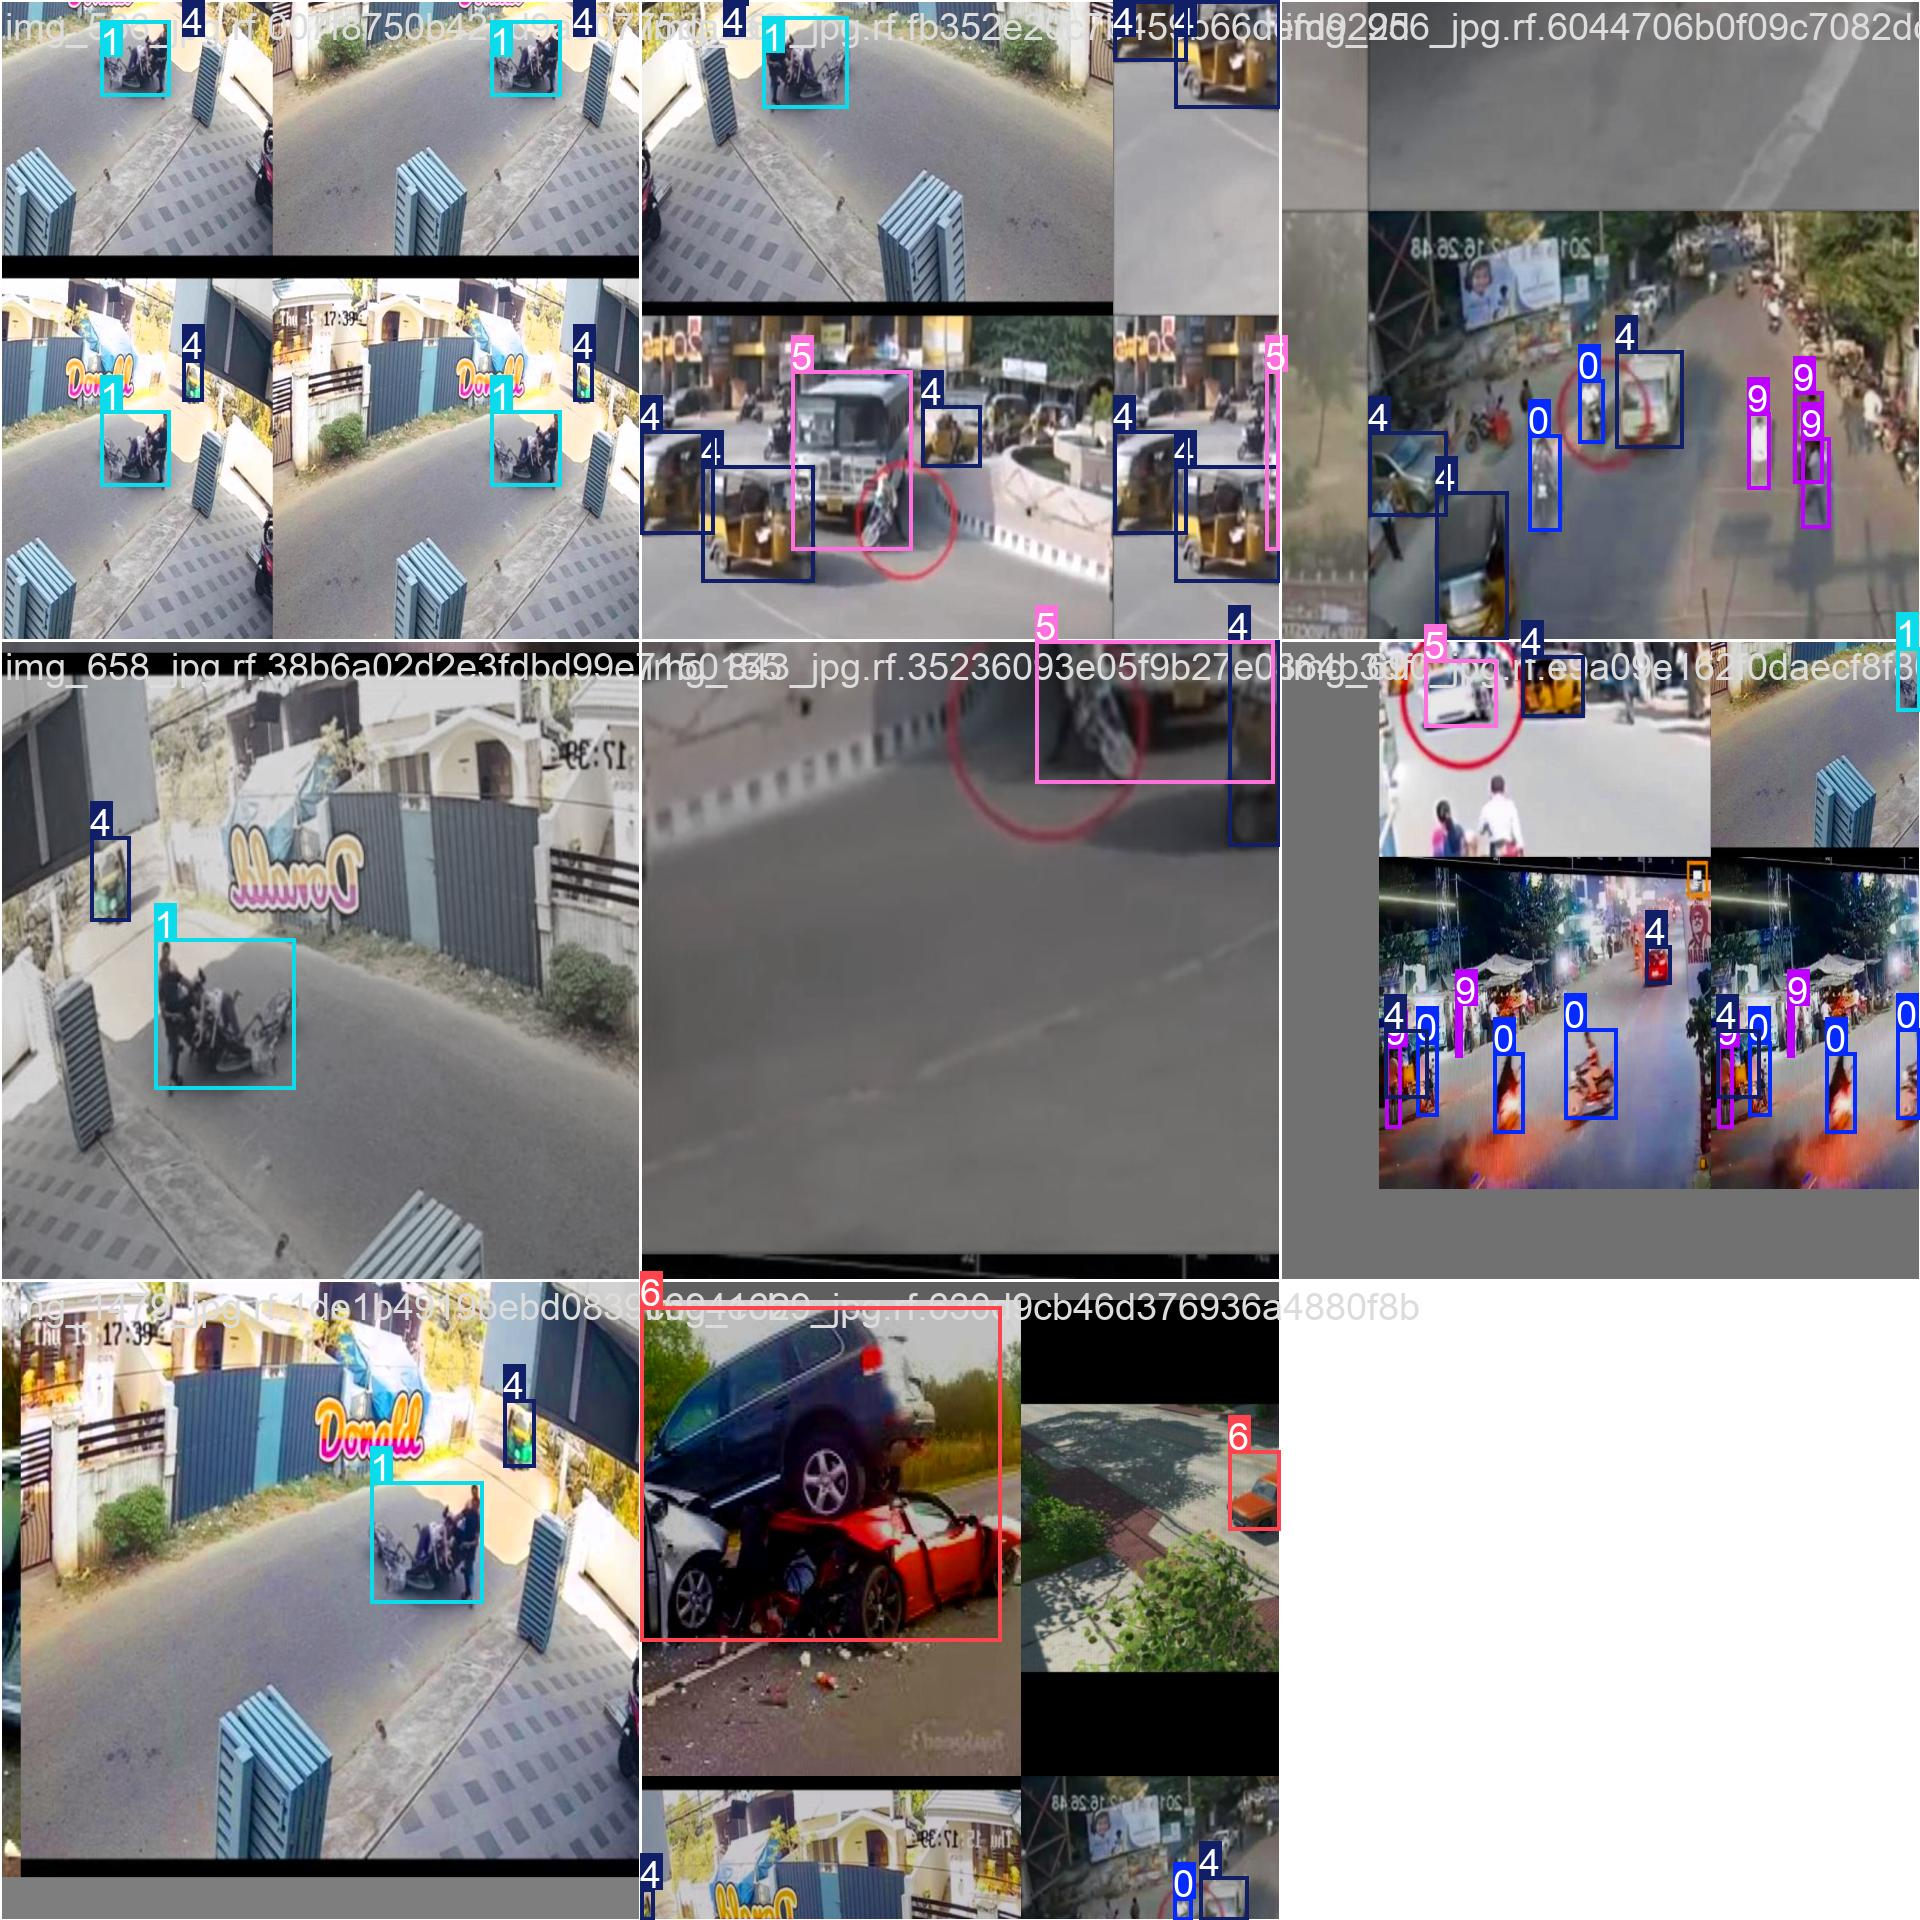
\includegraphics[width=\linewidth]{results/detection/yolo26_baseline/train_batch0.jpg}\end{minipage}
\begin{minipage}{0.32\textwidth}\centering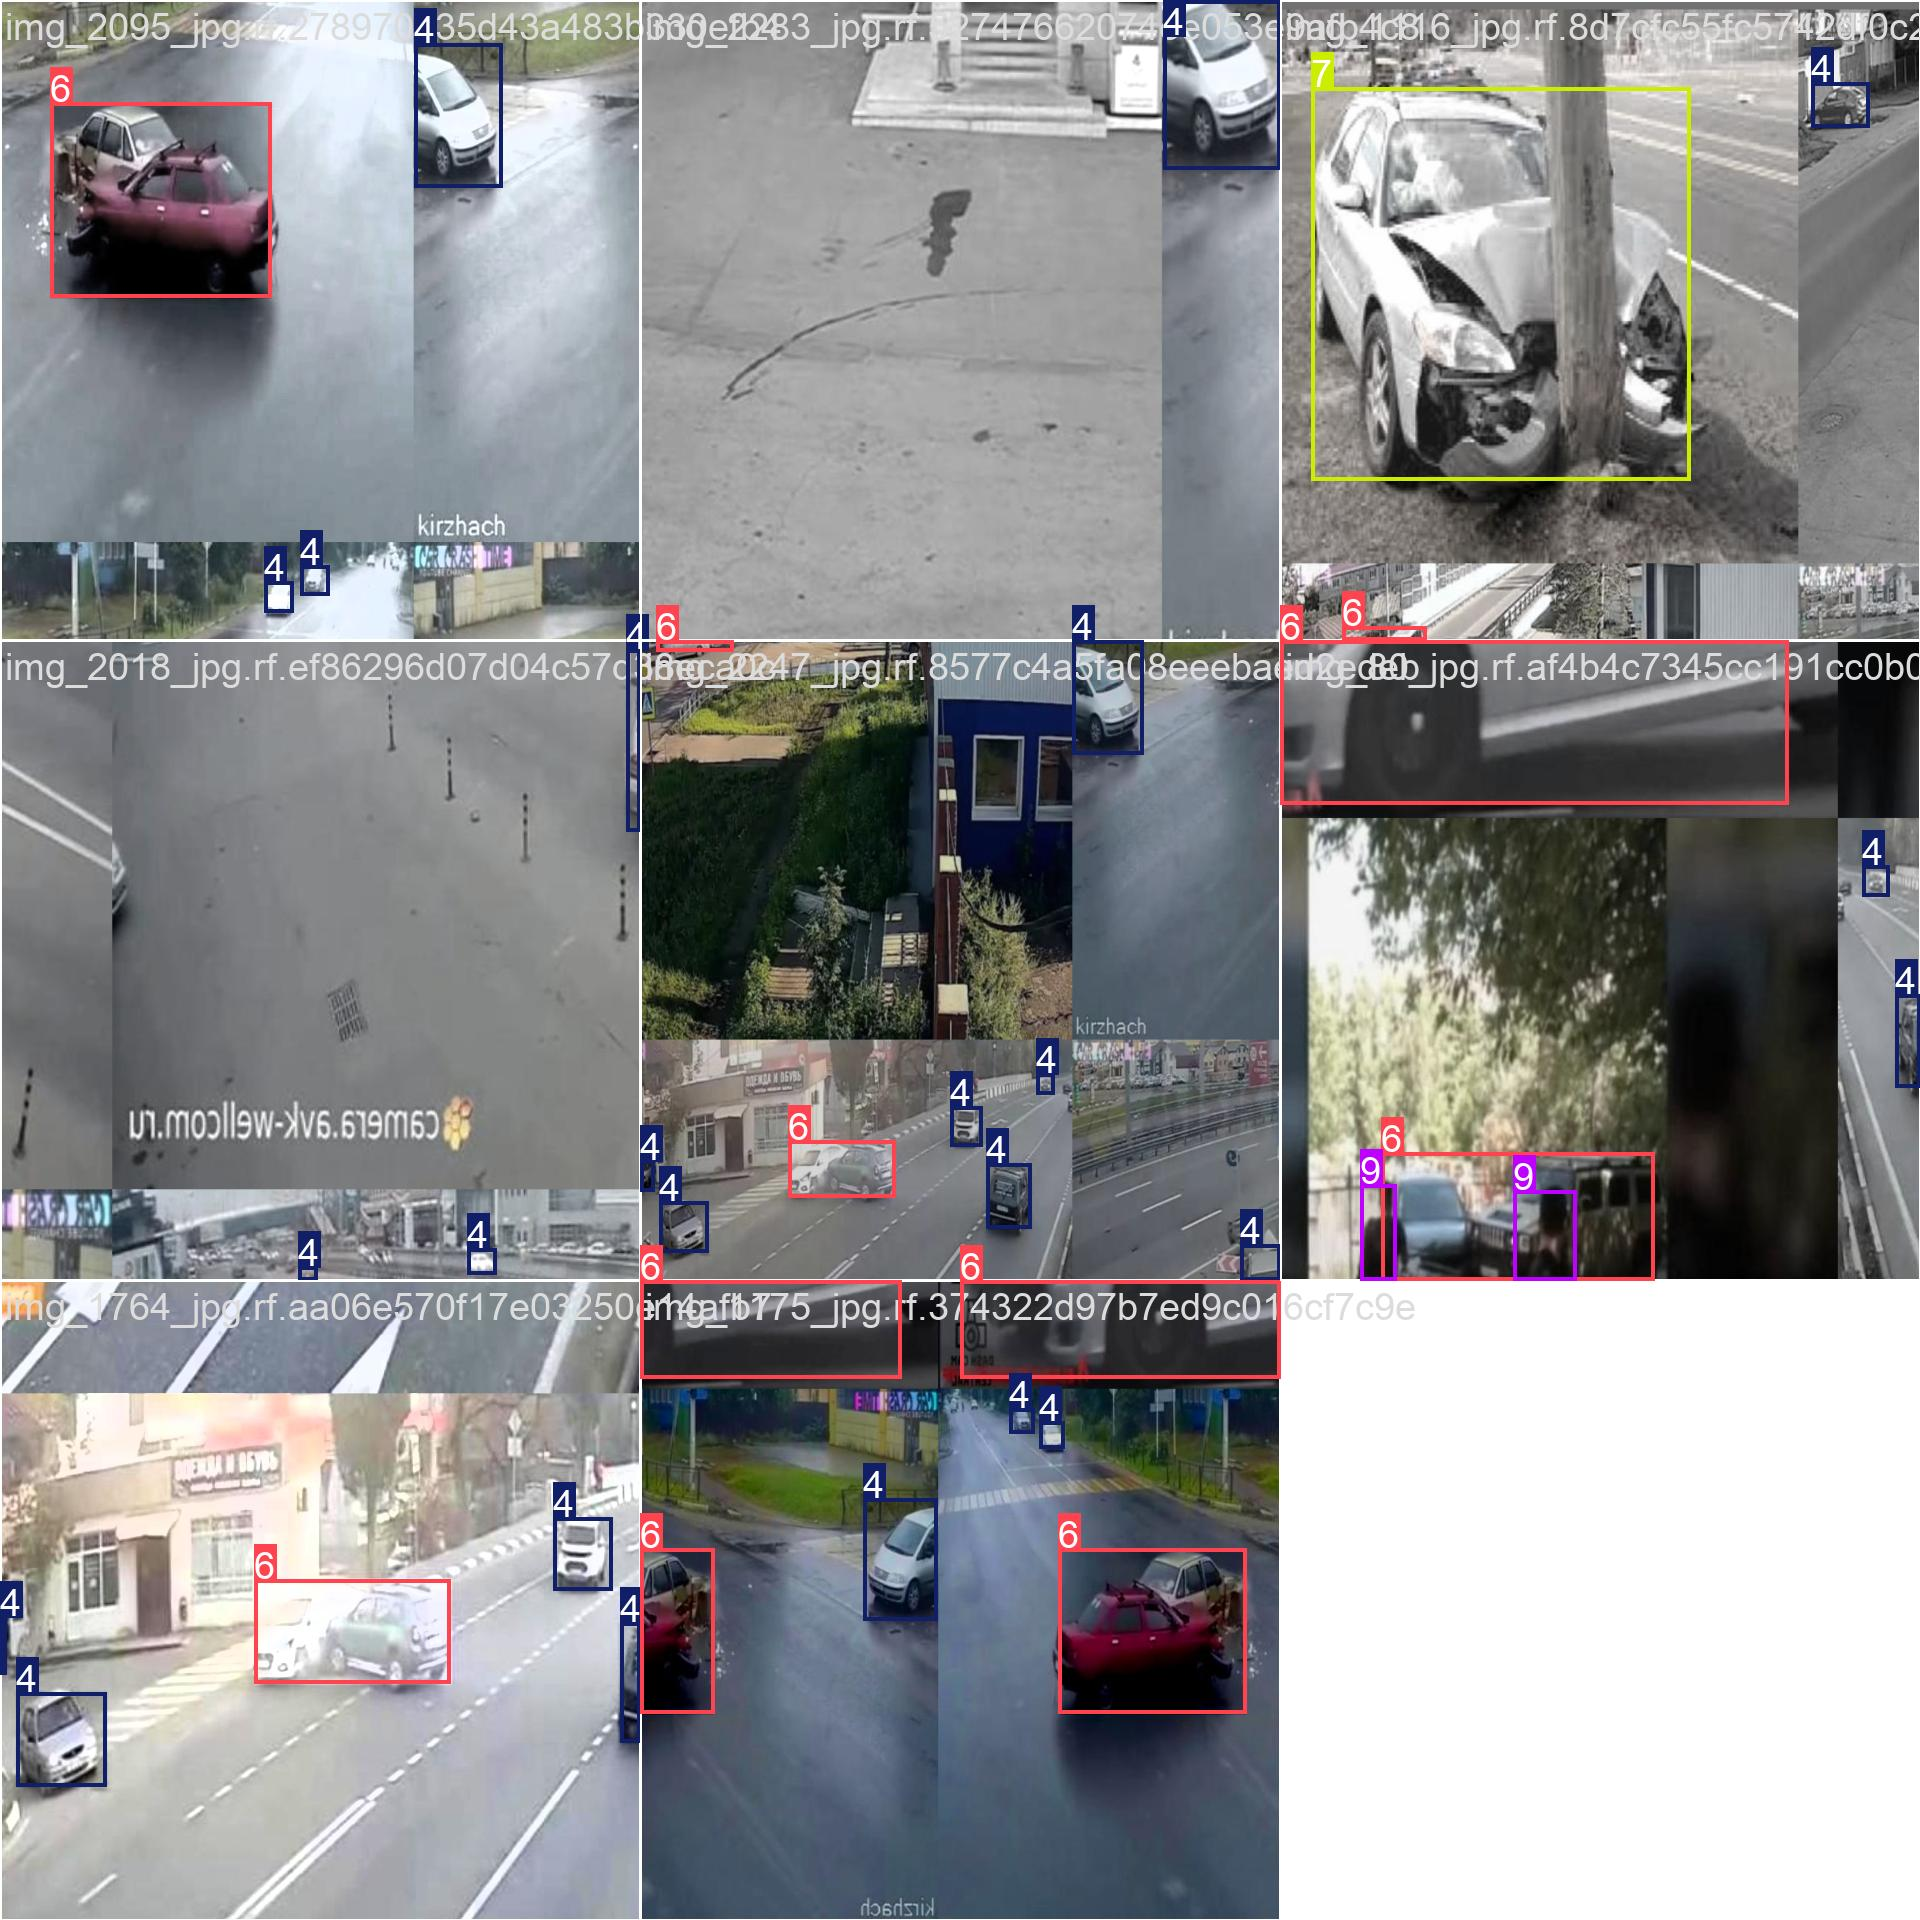
\includegraphics[width=\linewidth]{results/detection/yolo26_baseline/train_batch1.jpg}\end{minipage}
\begin{minipage}{0.32\textwidth}\centering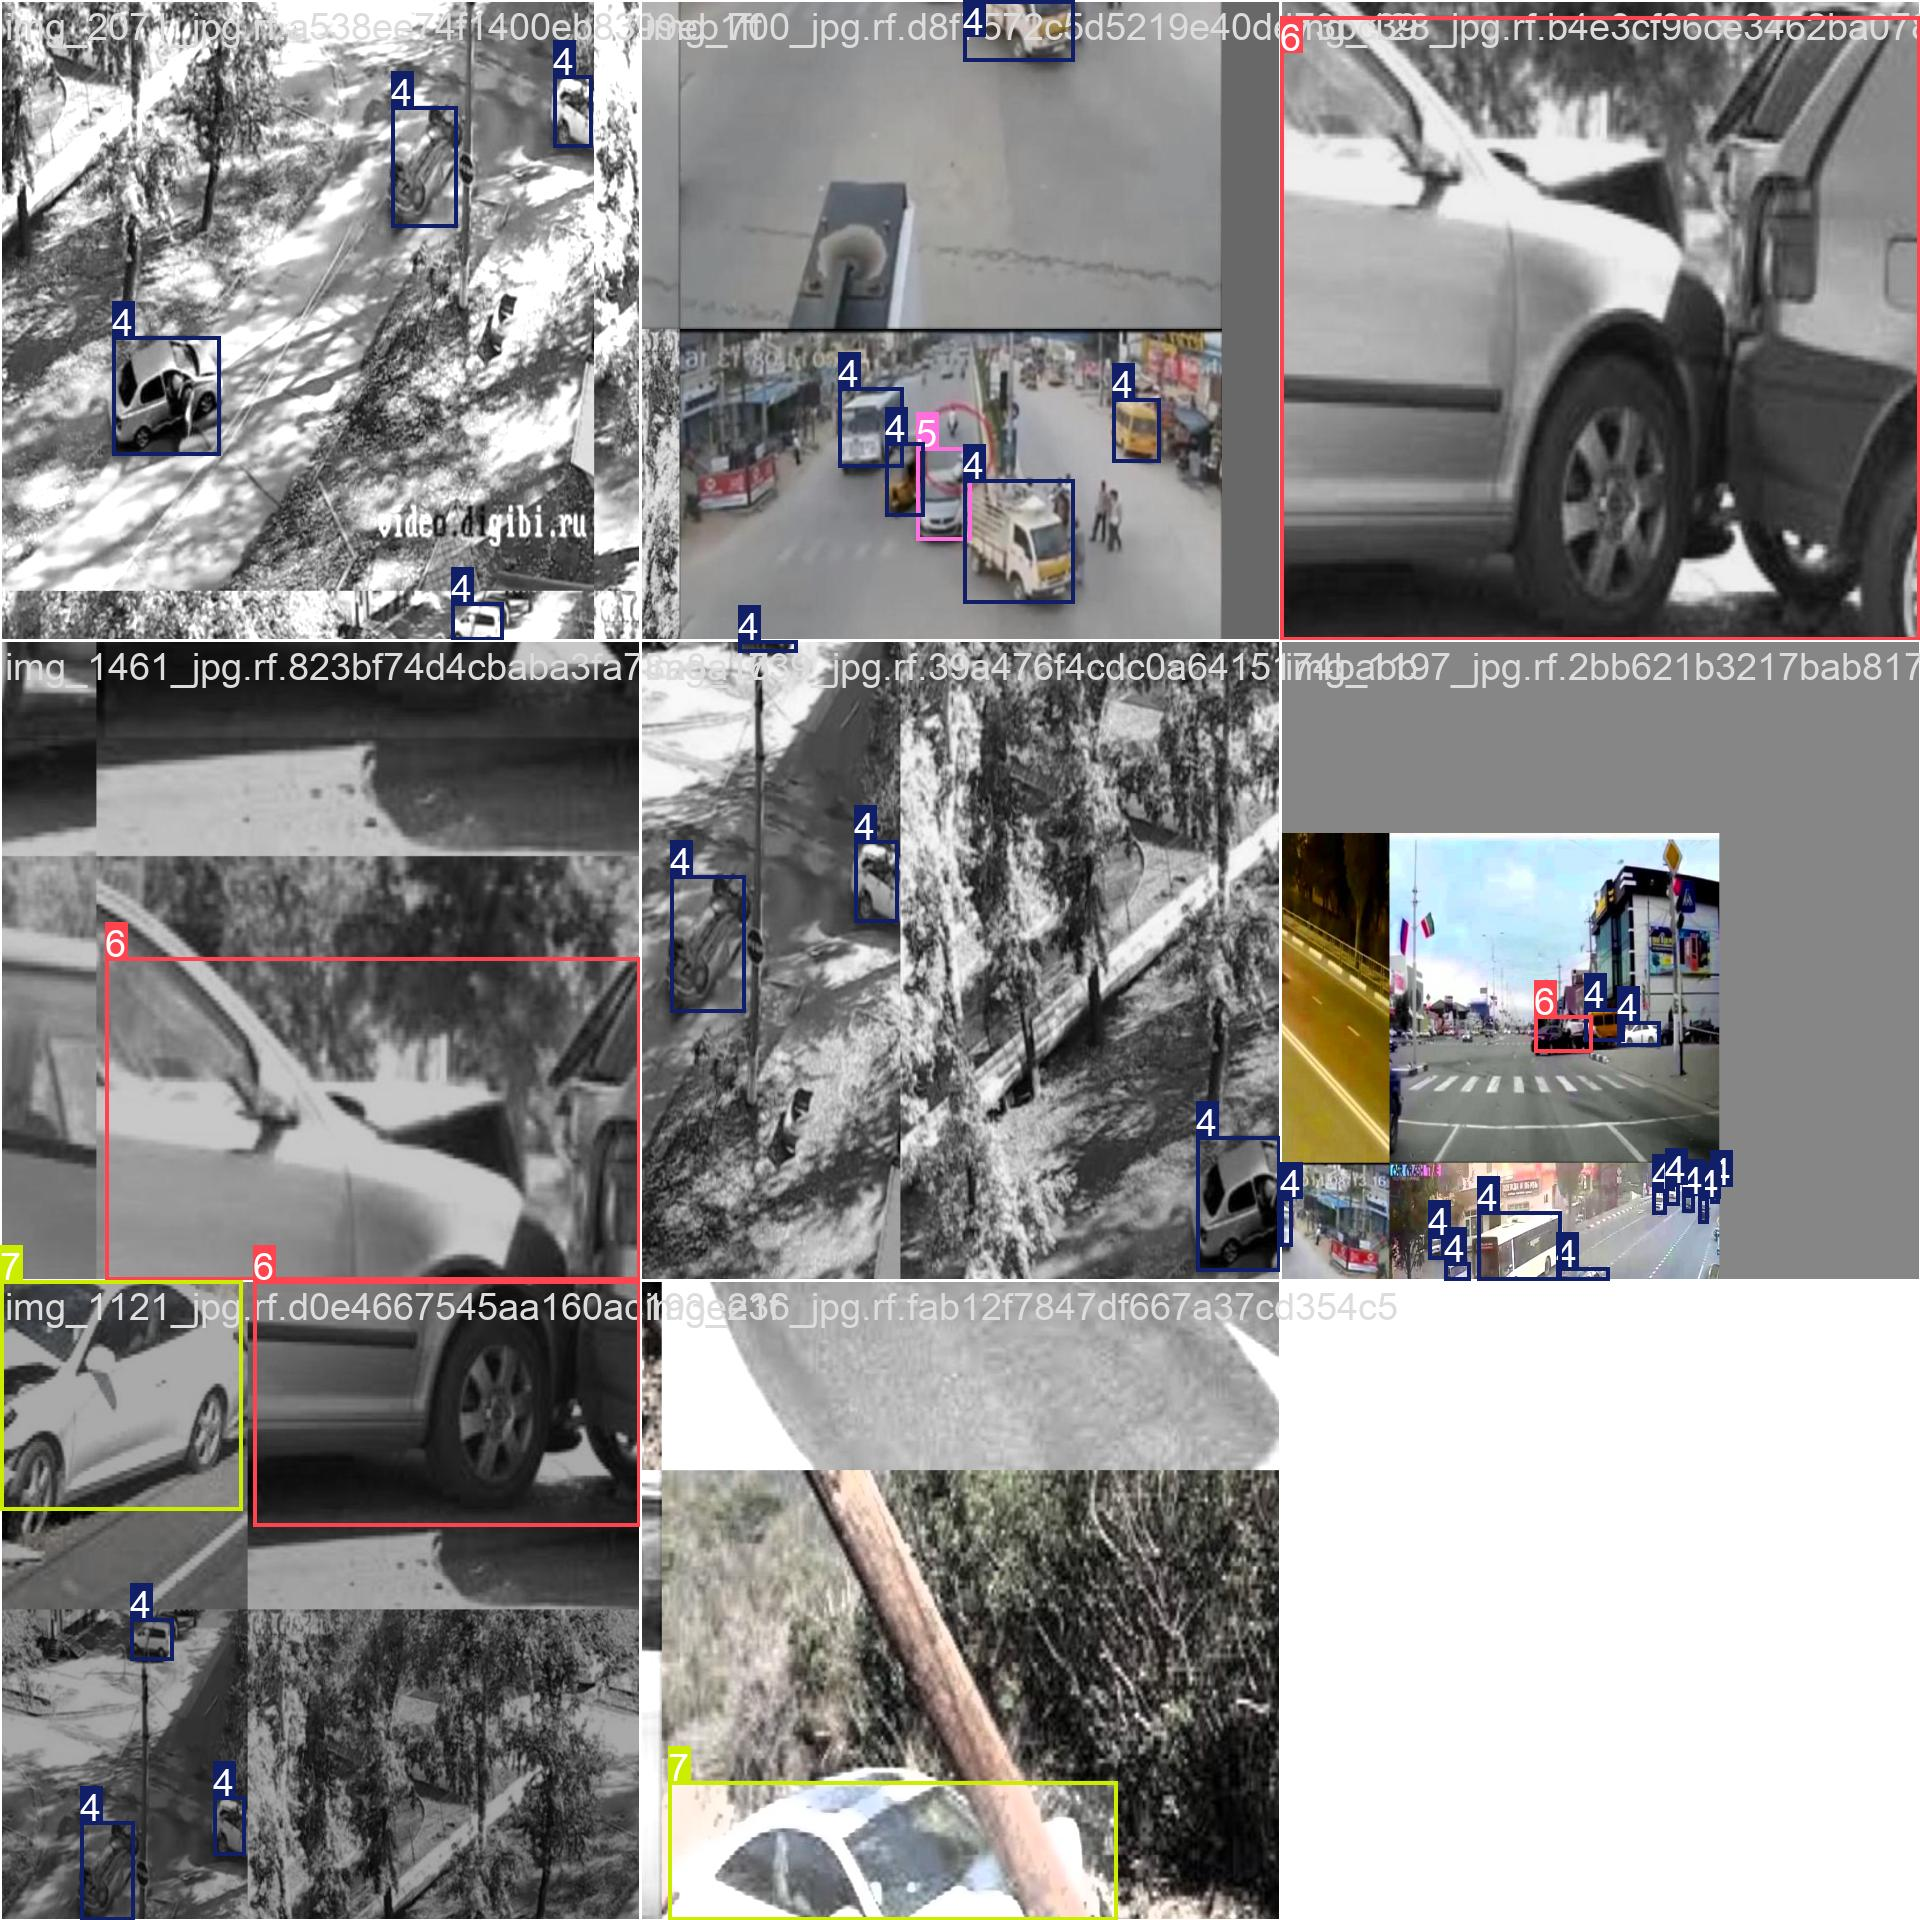
\includegraphics[width=\linewidth]{results/detection/yolo26_baseline/train_batch2.jpg}\end{minipage}
\caption{Saved training-batch previews for Accident Detection.}
\end{figure}
\begin{figure}[t]\centering
\begin{minipage}{0.32\textwidth}\centering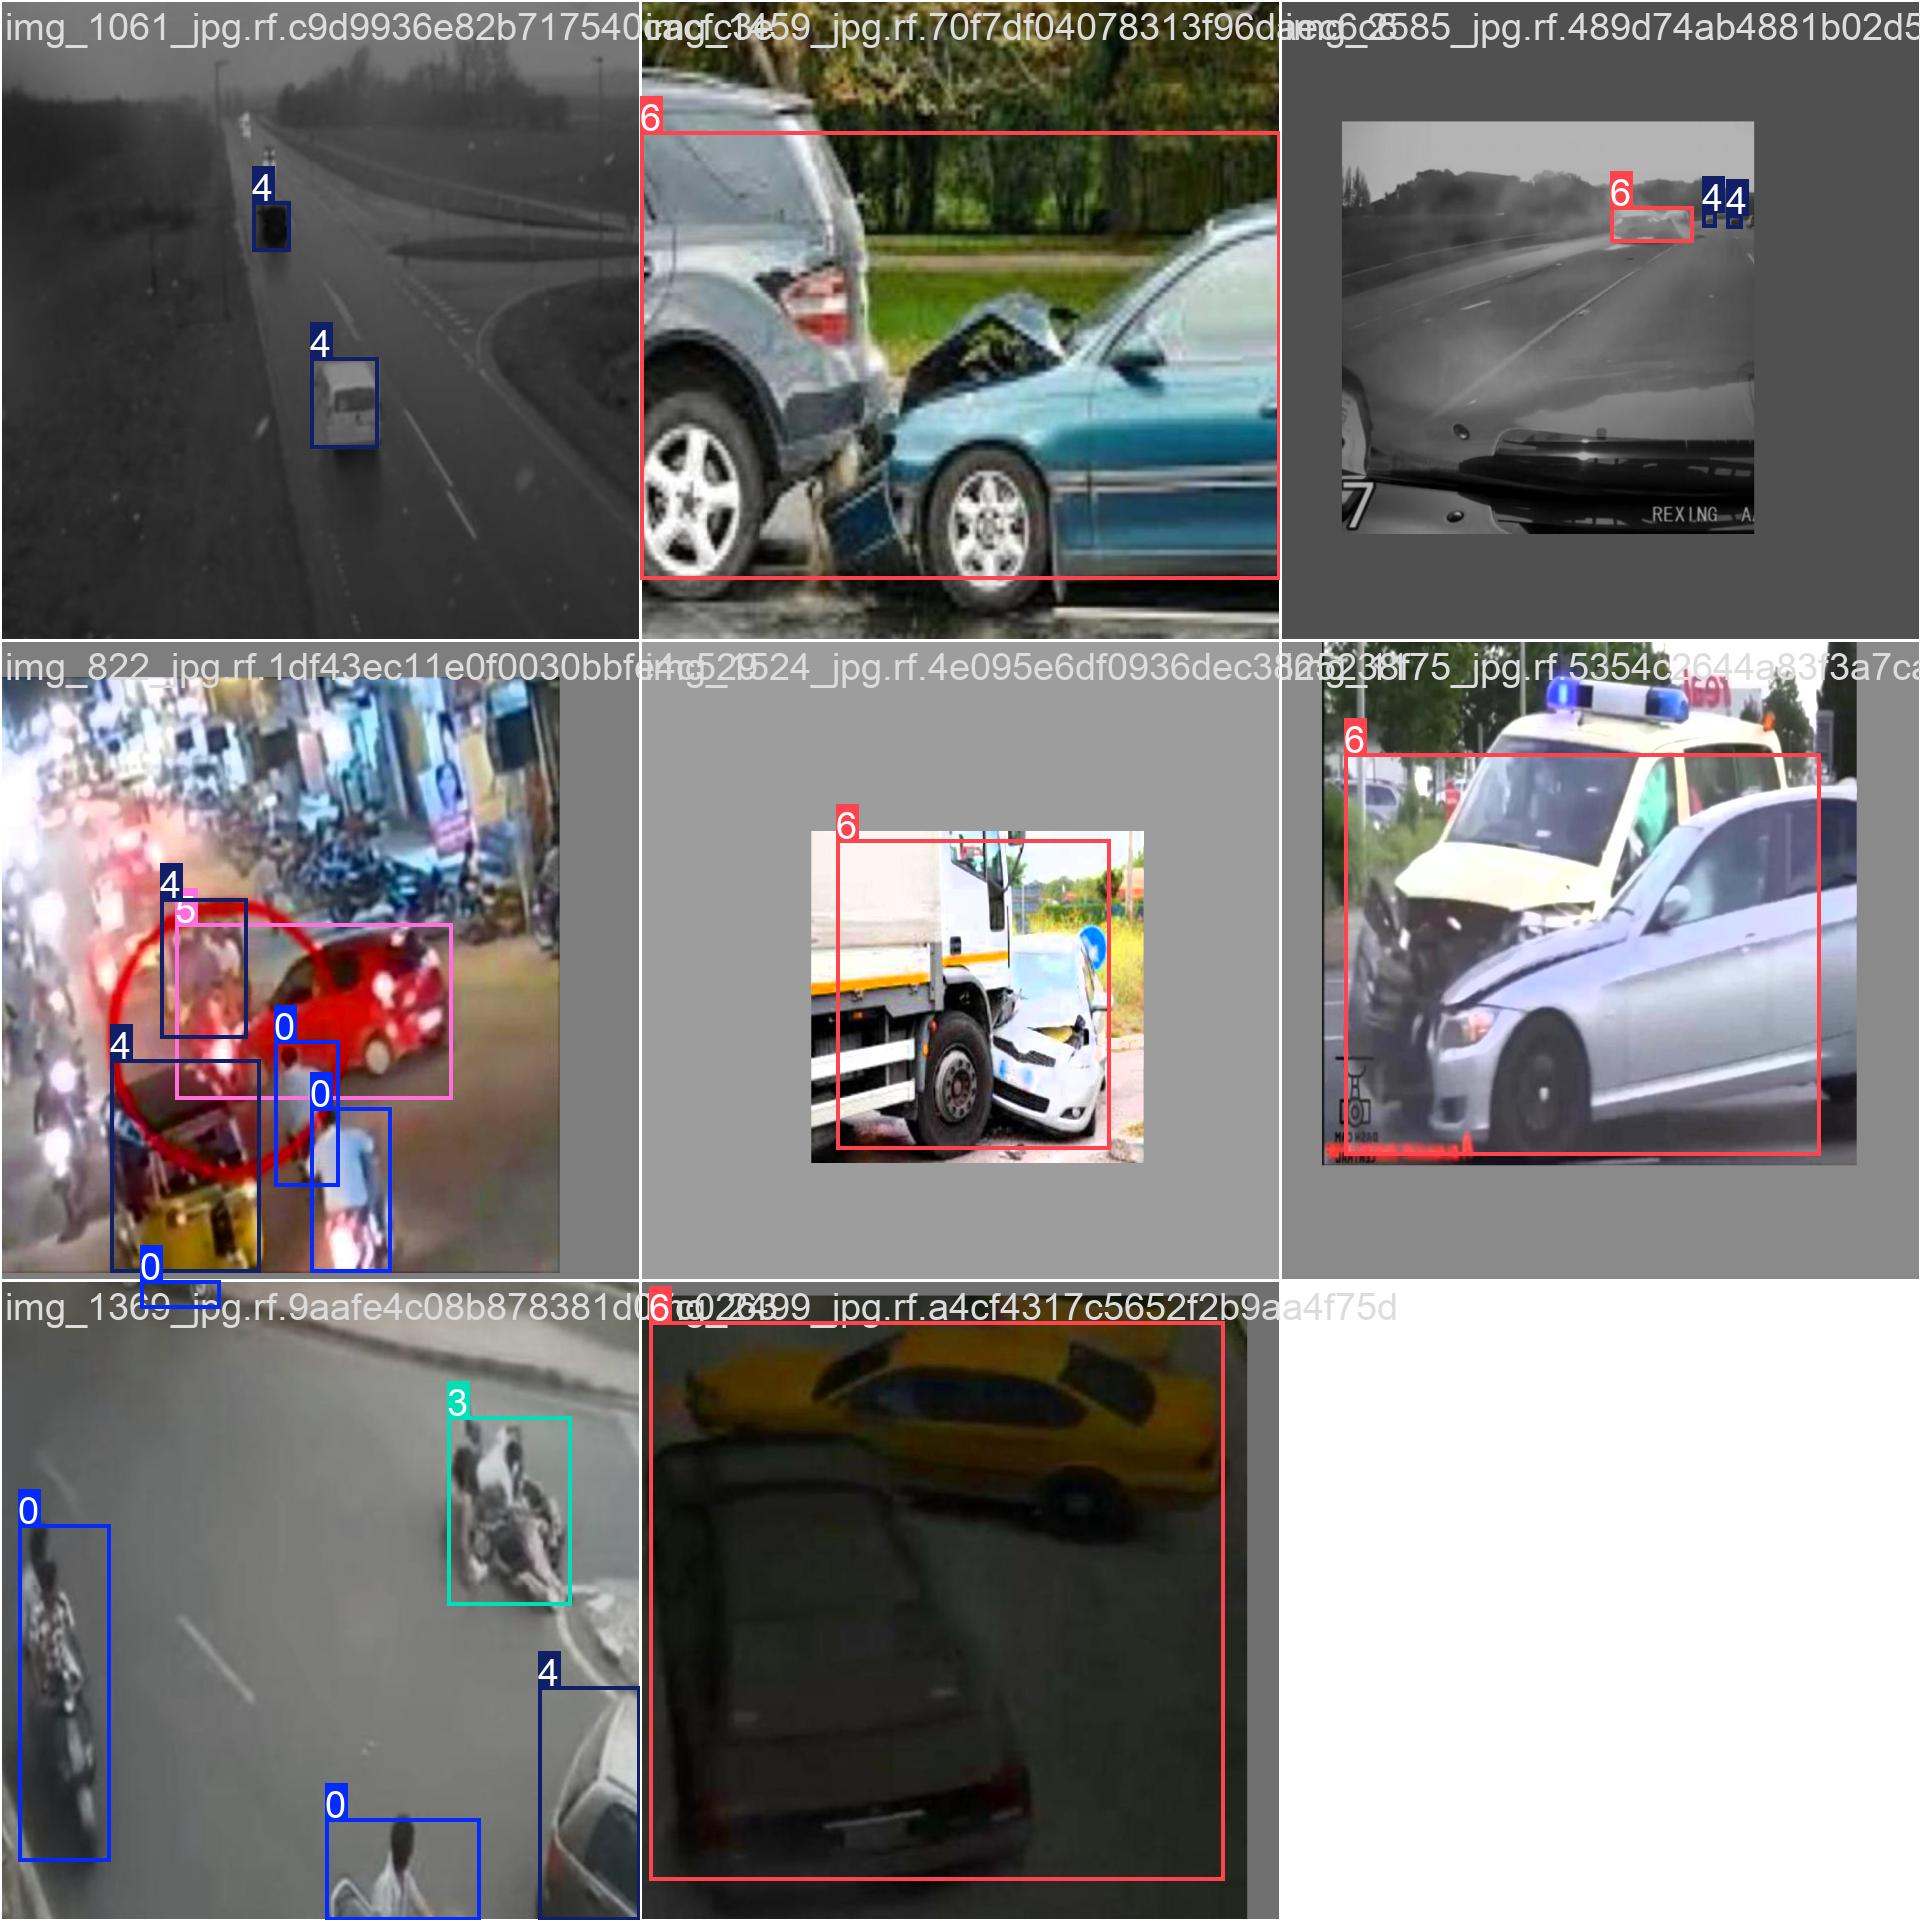
\includegraphics[width=\linewidth]{results/detection/yolo26_baseline/train_batch65880.jpg}\end{minipage}
\begin{minipage}{0.32\textwidth}\centering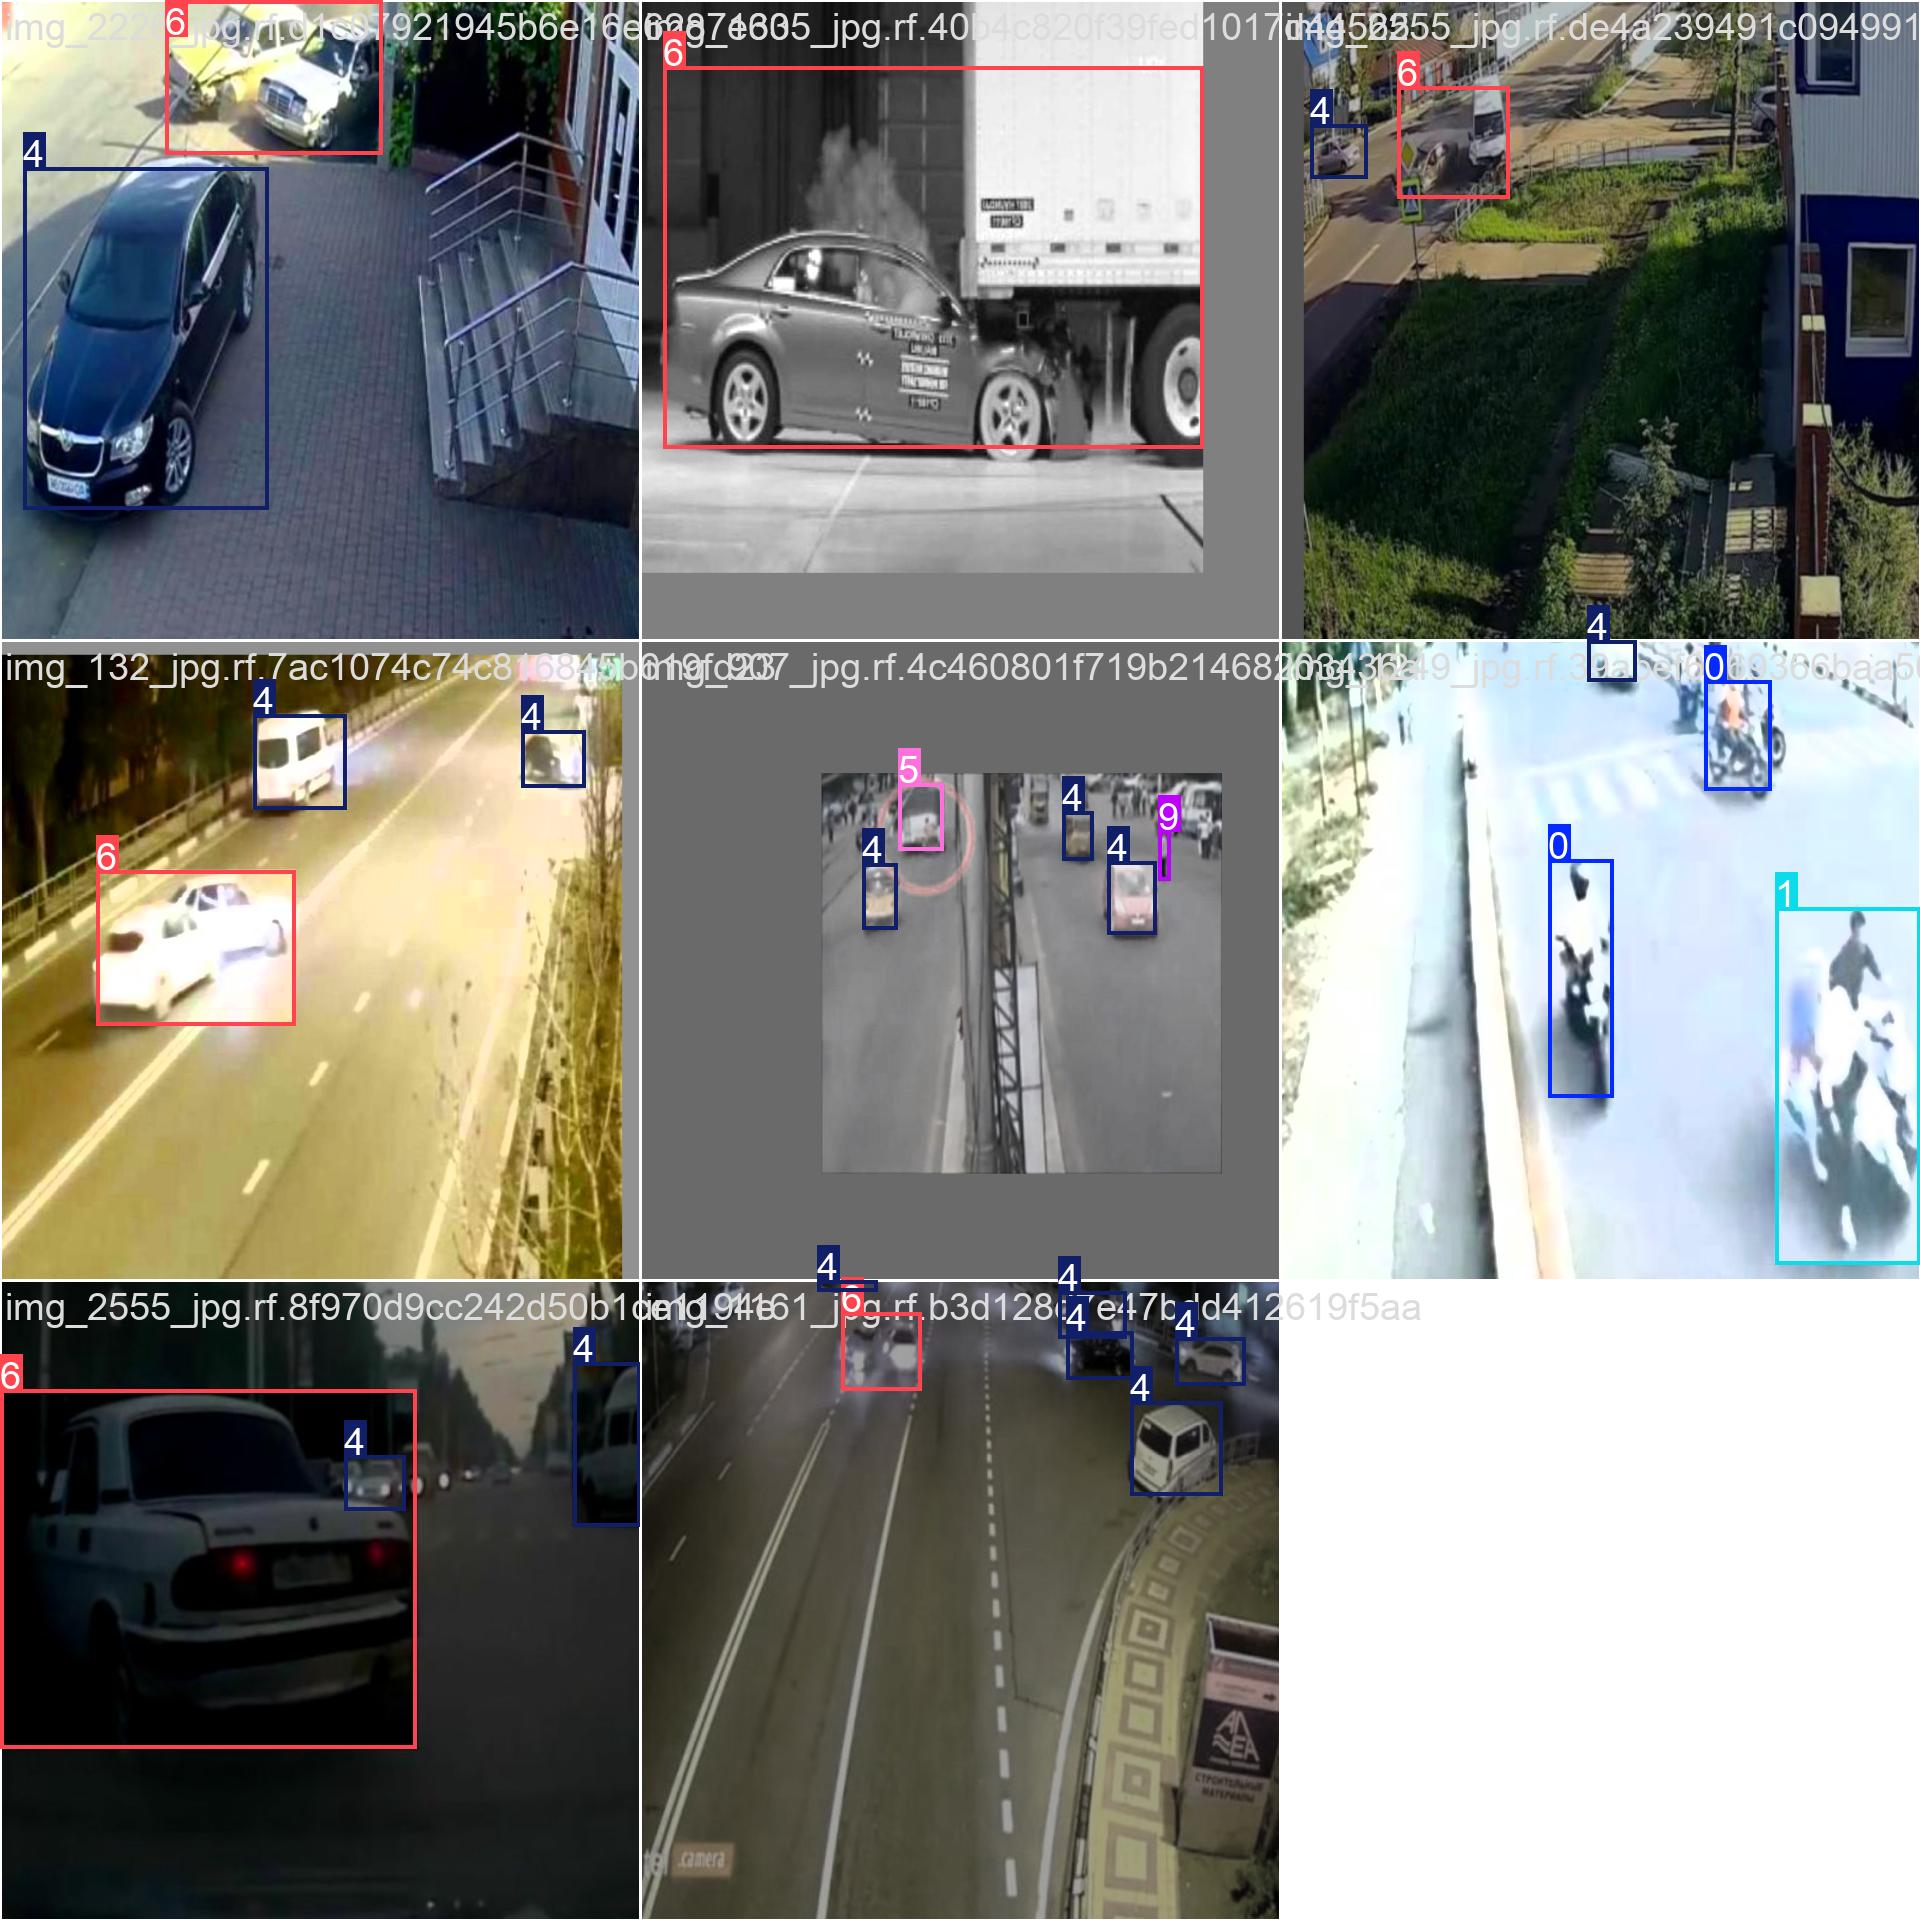
\includegraphics[width=\linewidth]{results/detection/yolo26_baseline/train_batch65881.jpg}\end{minipage}
\begin{minipage}{0.32\textwidth}\centering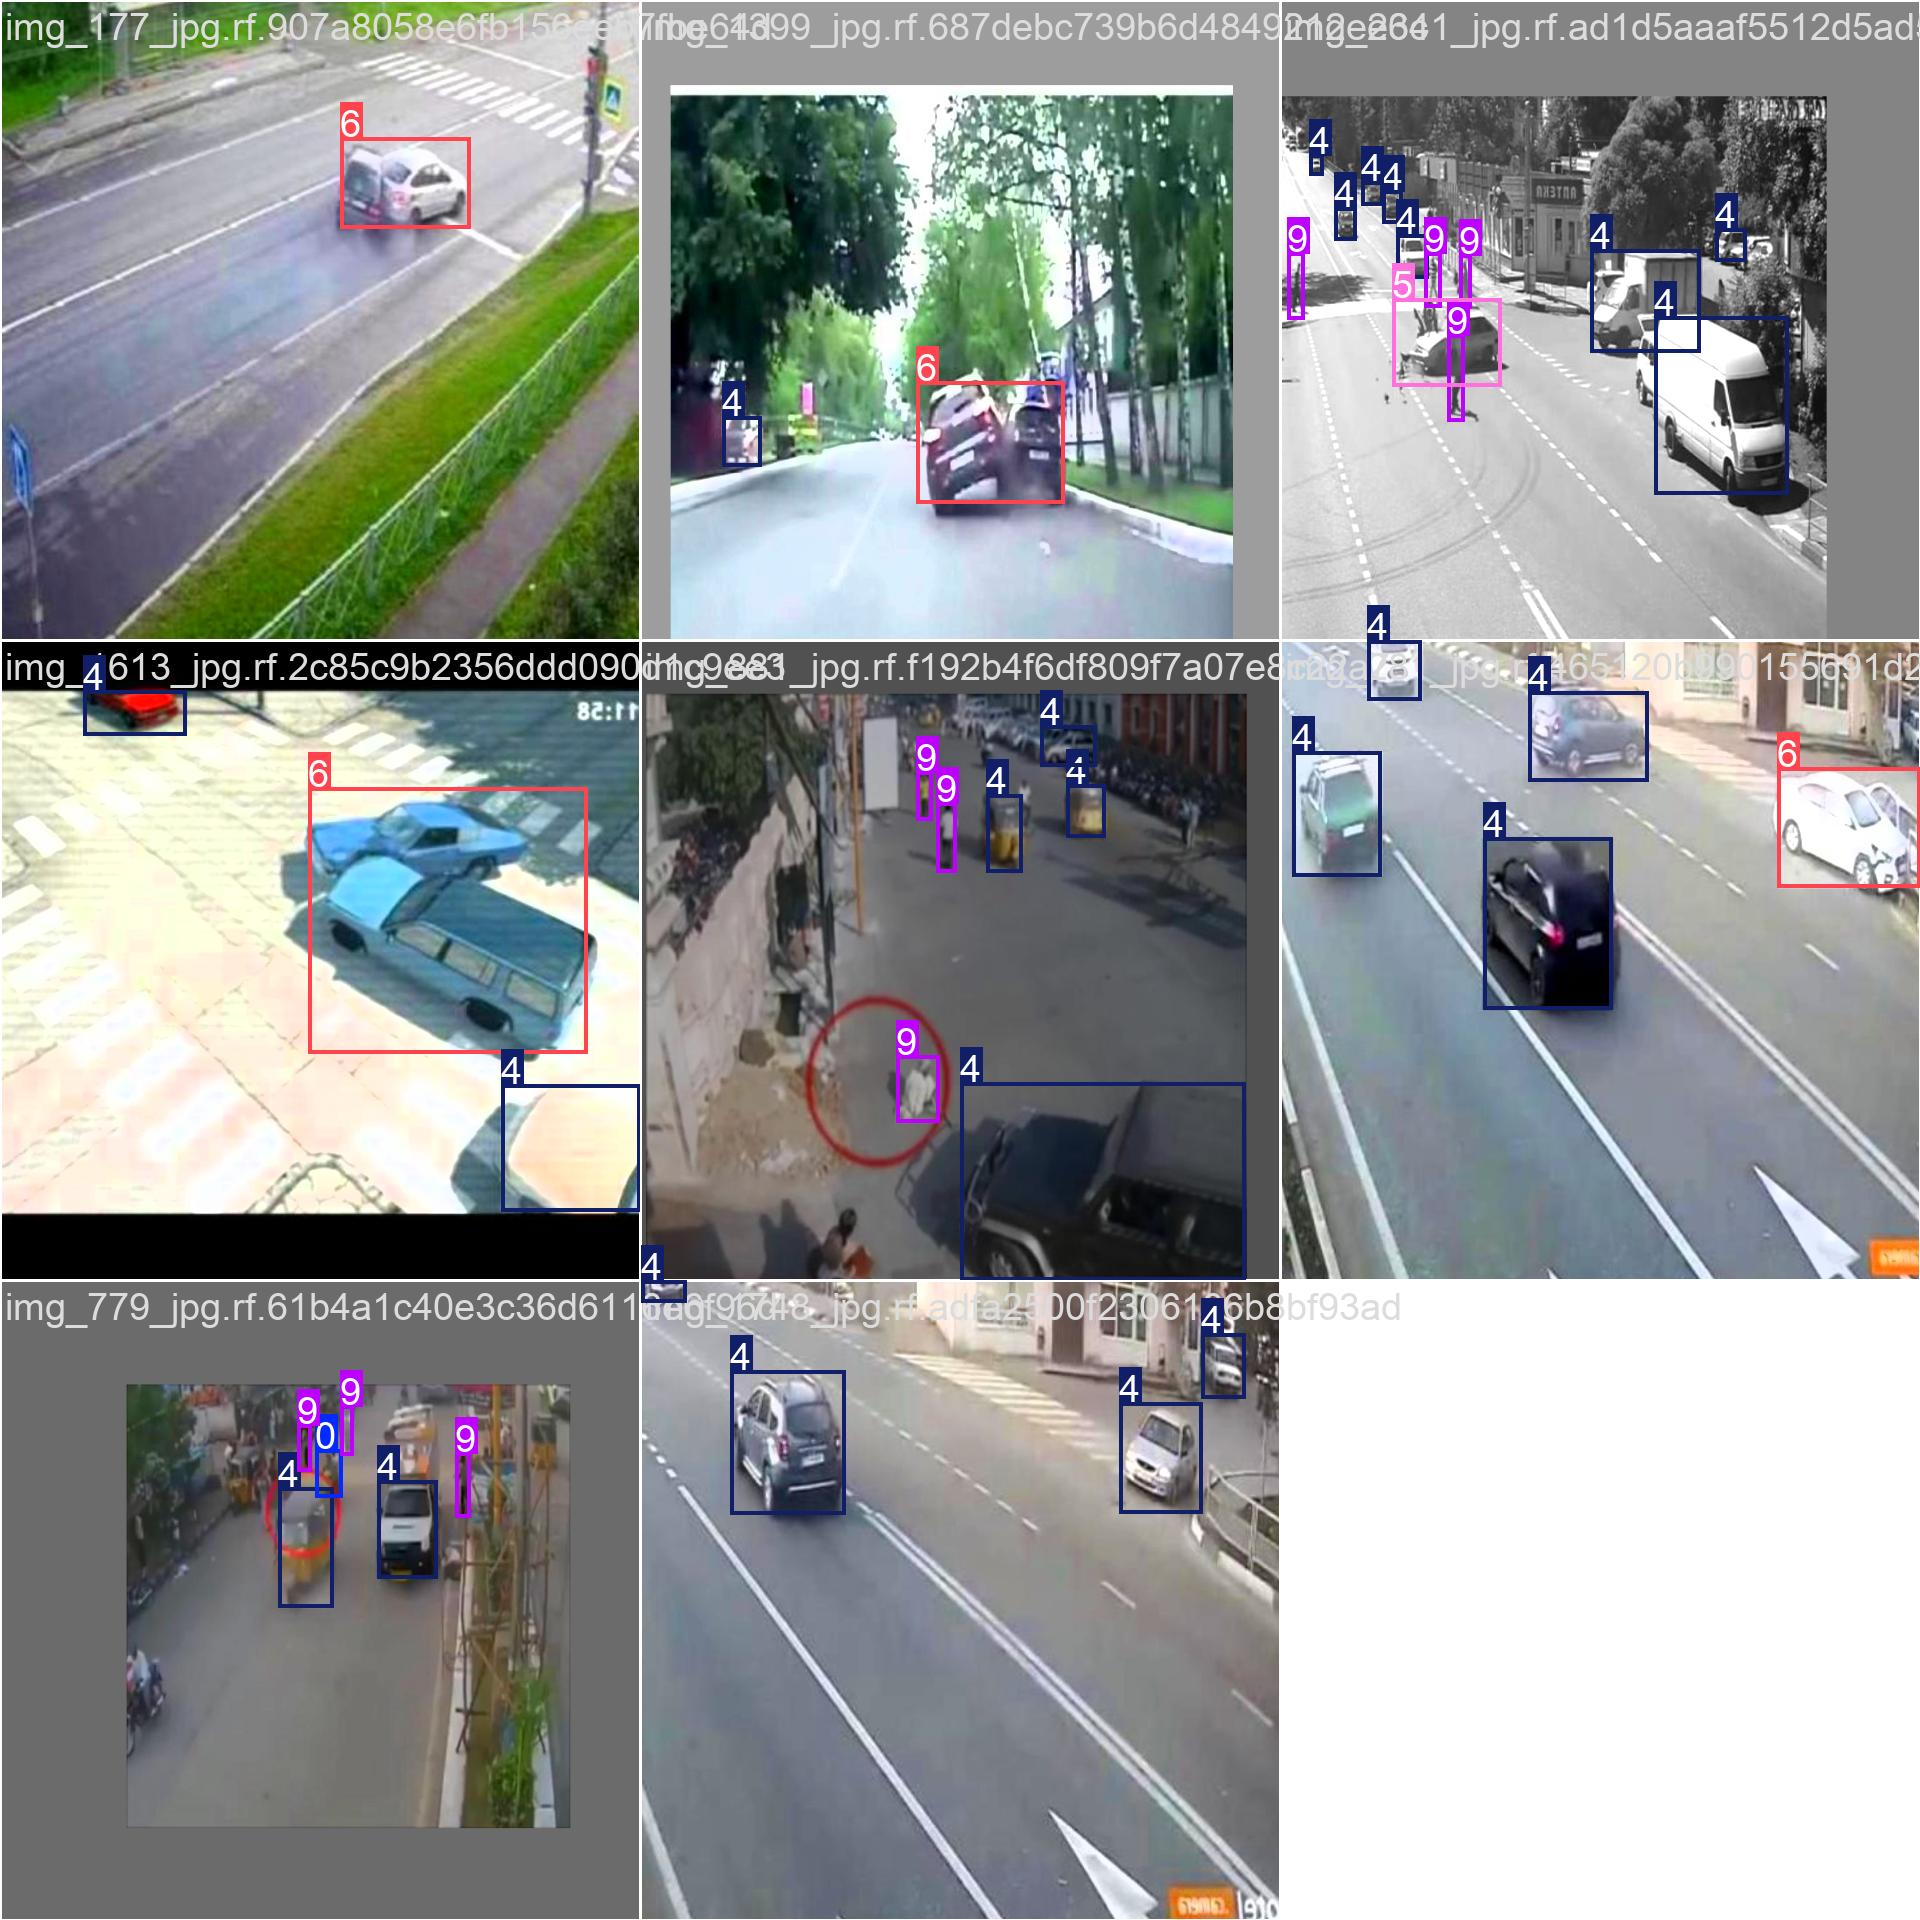
\includegraphics[width=\linewidth]{results/detection/yolo26_baseline/train_batch65882.jpg}\end{minipage}
\caption{Saved training-batch previews for Accident Detection.}
\end{figure}
\begin{figure}[t]\centering
\begin{minipage}{0.32\textwidth}\centering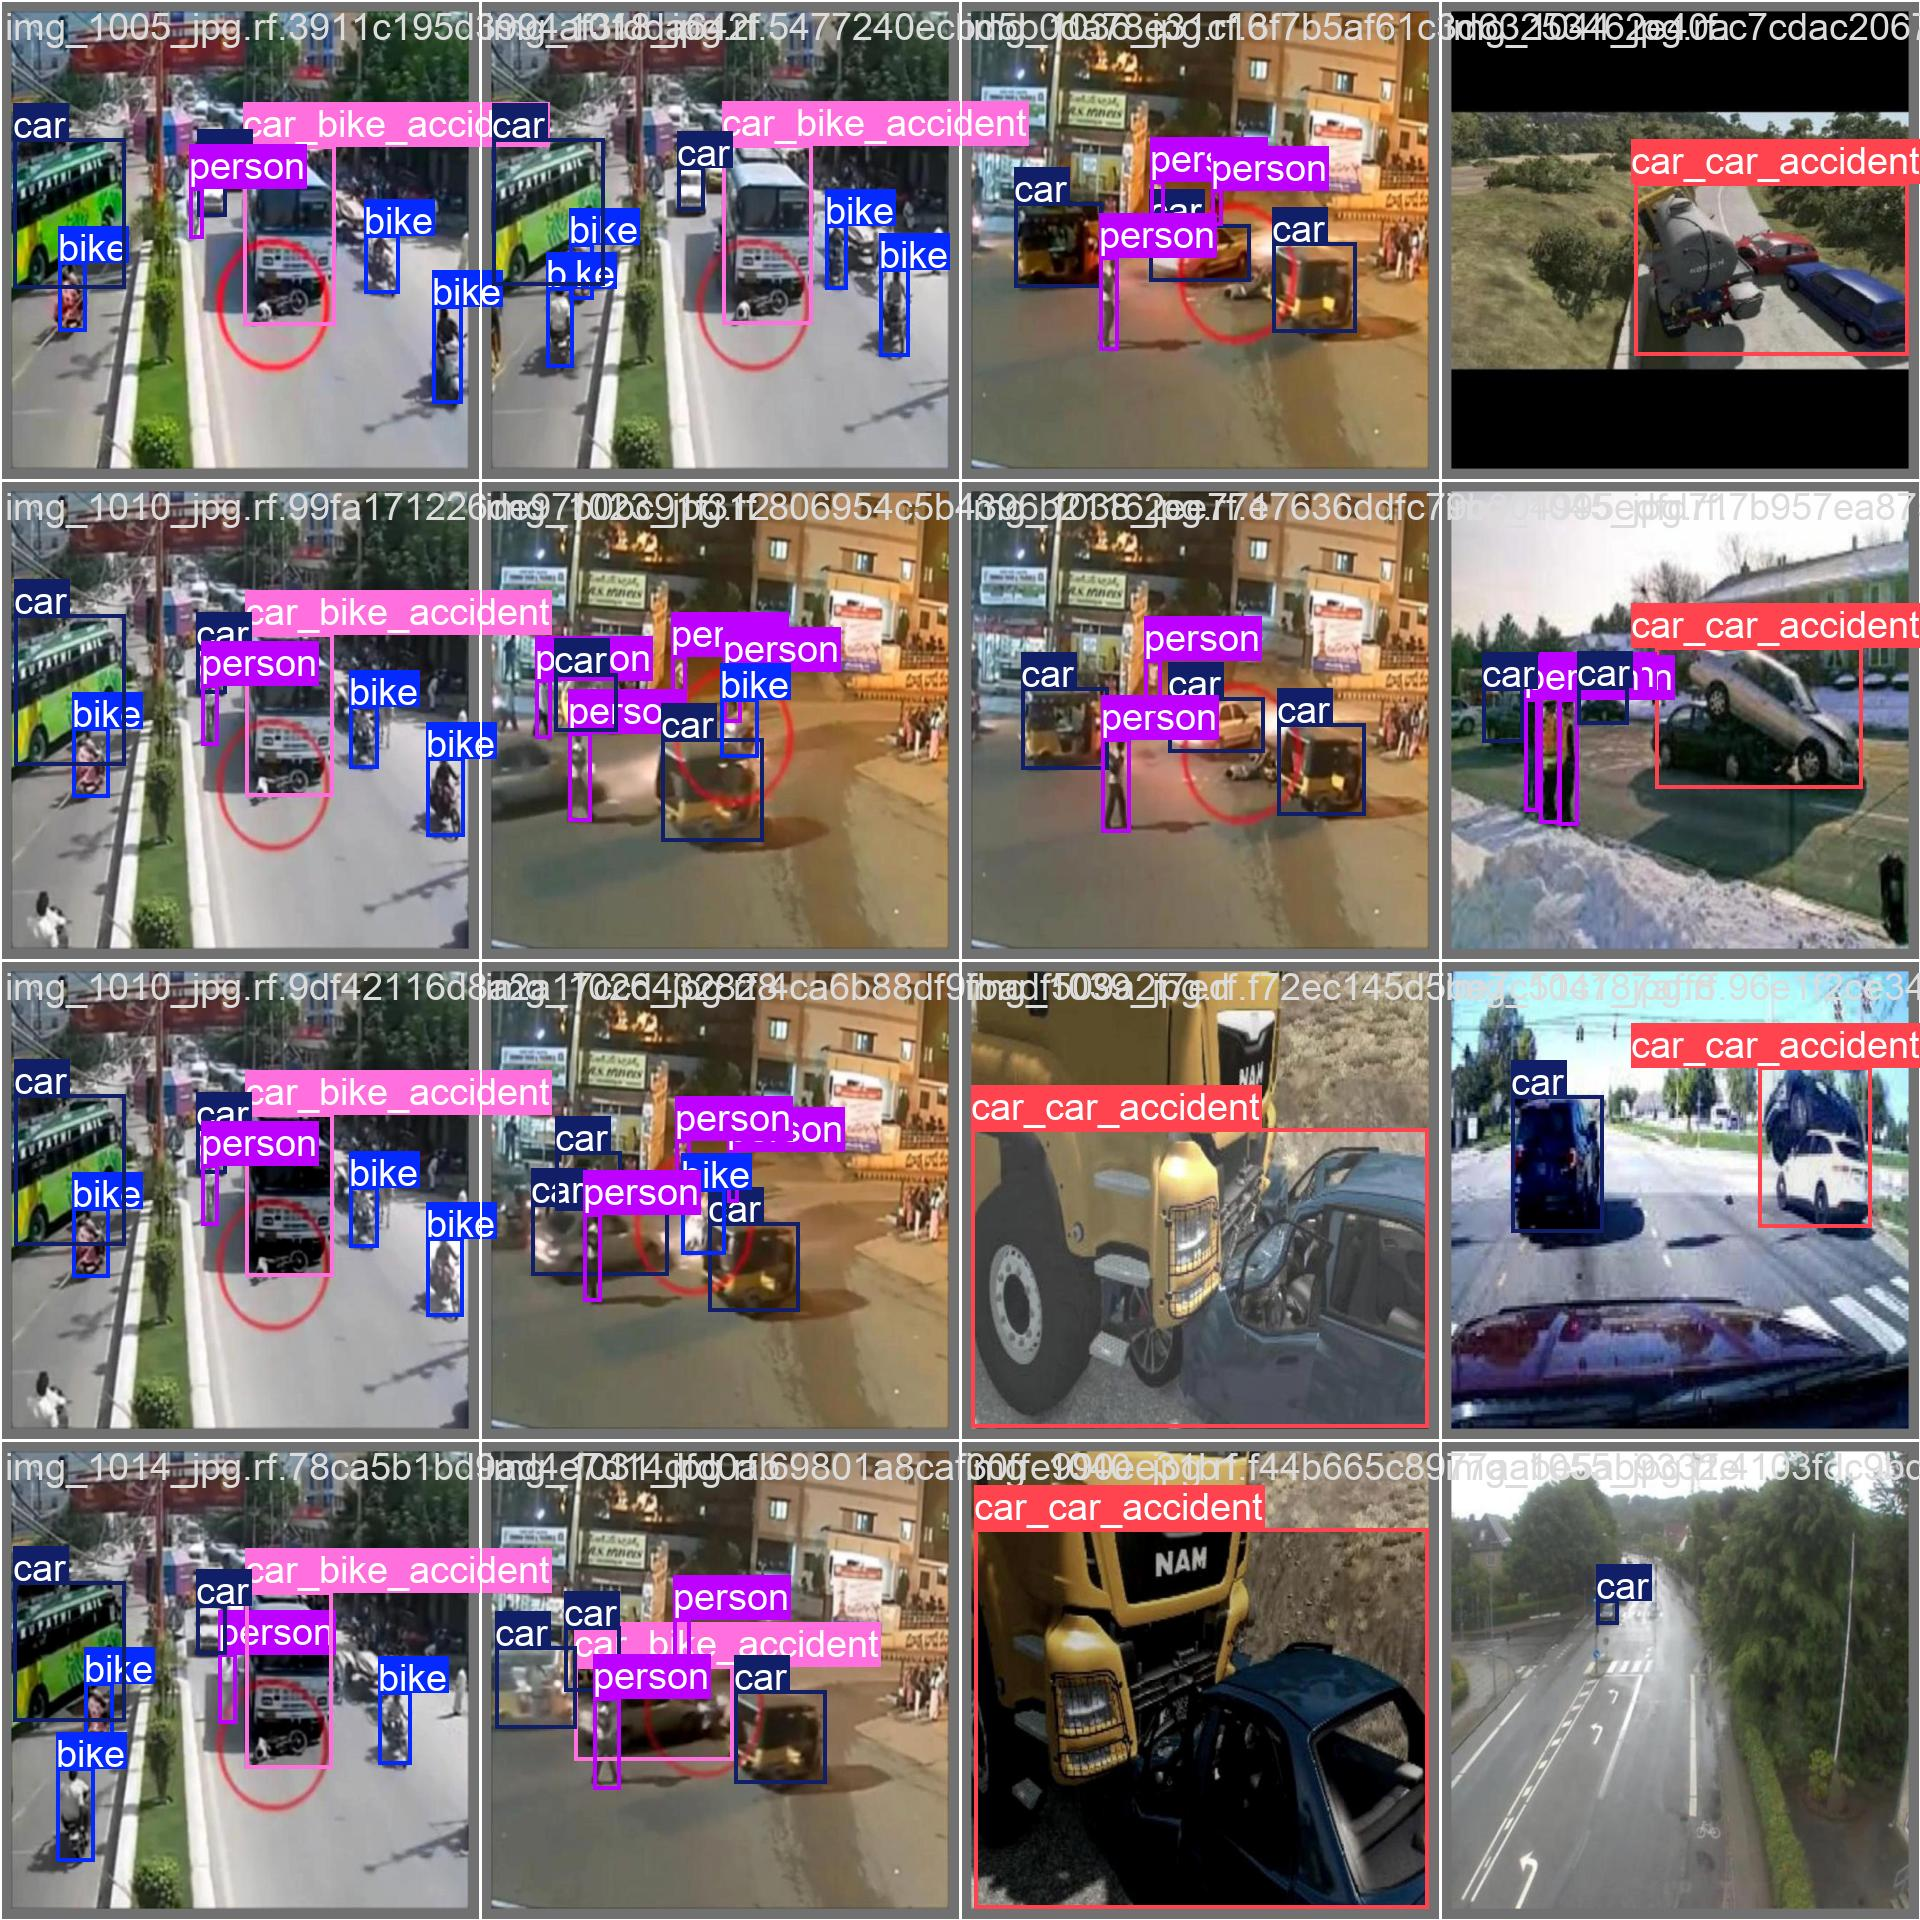
\includegraphics[width=\linewidth]{results/detection/yolo26_baseline/val_batch0_labels.jpg}\end{minipage}
\begin{minipage}{0.32\textwidth}\centering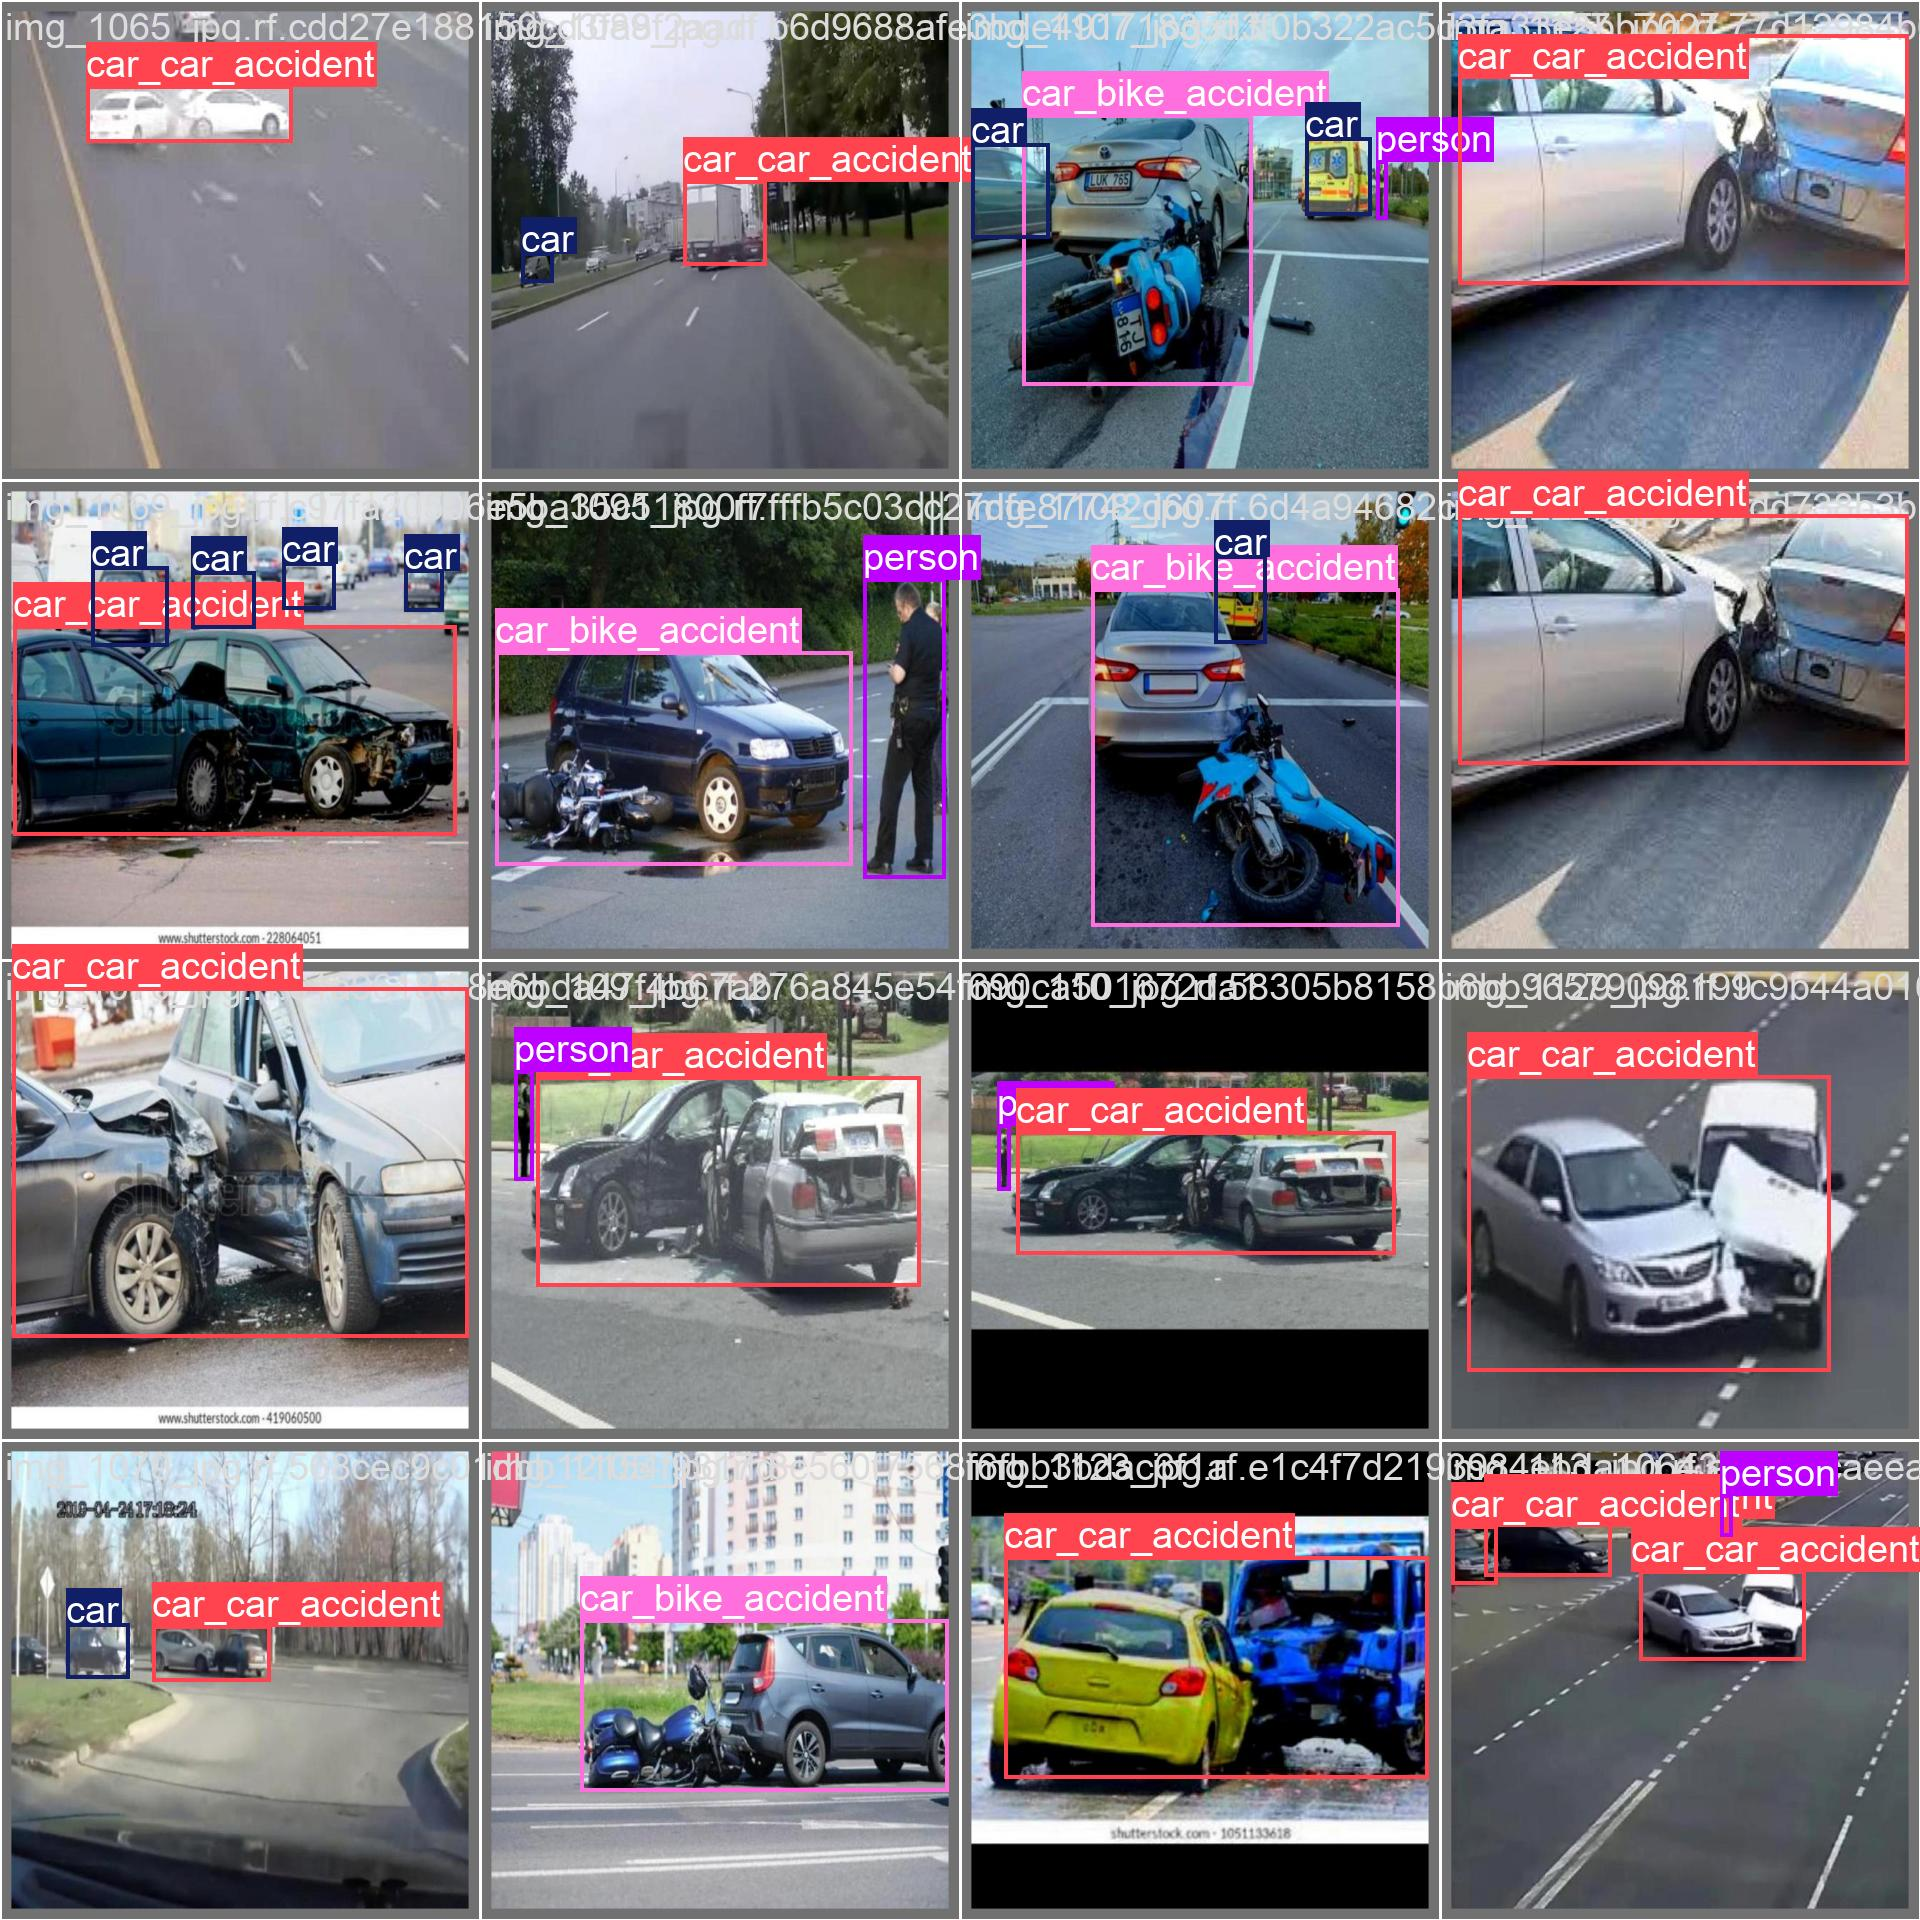
\includegraphics[width=\linewidth]{results/detection/yolo26_baseline/val_batch1_labels.jpg}\end{minipage}
\begin{minipage}{0.32\textwidth}\centering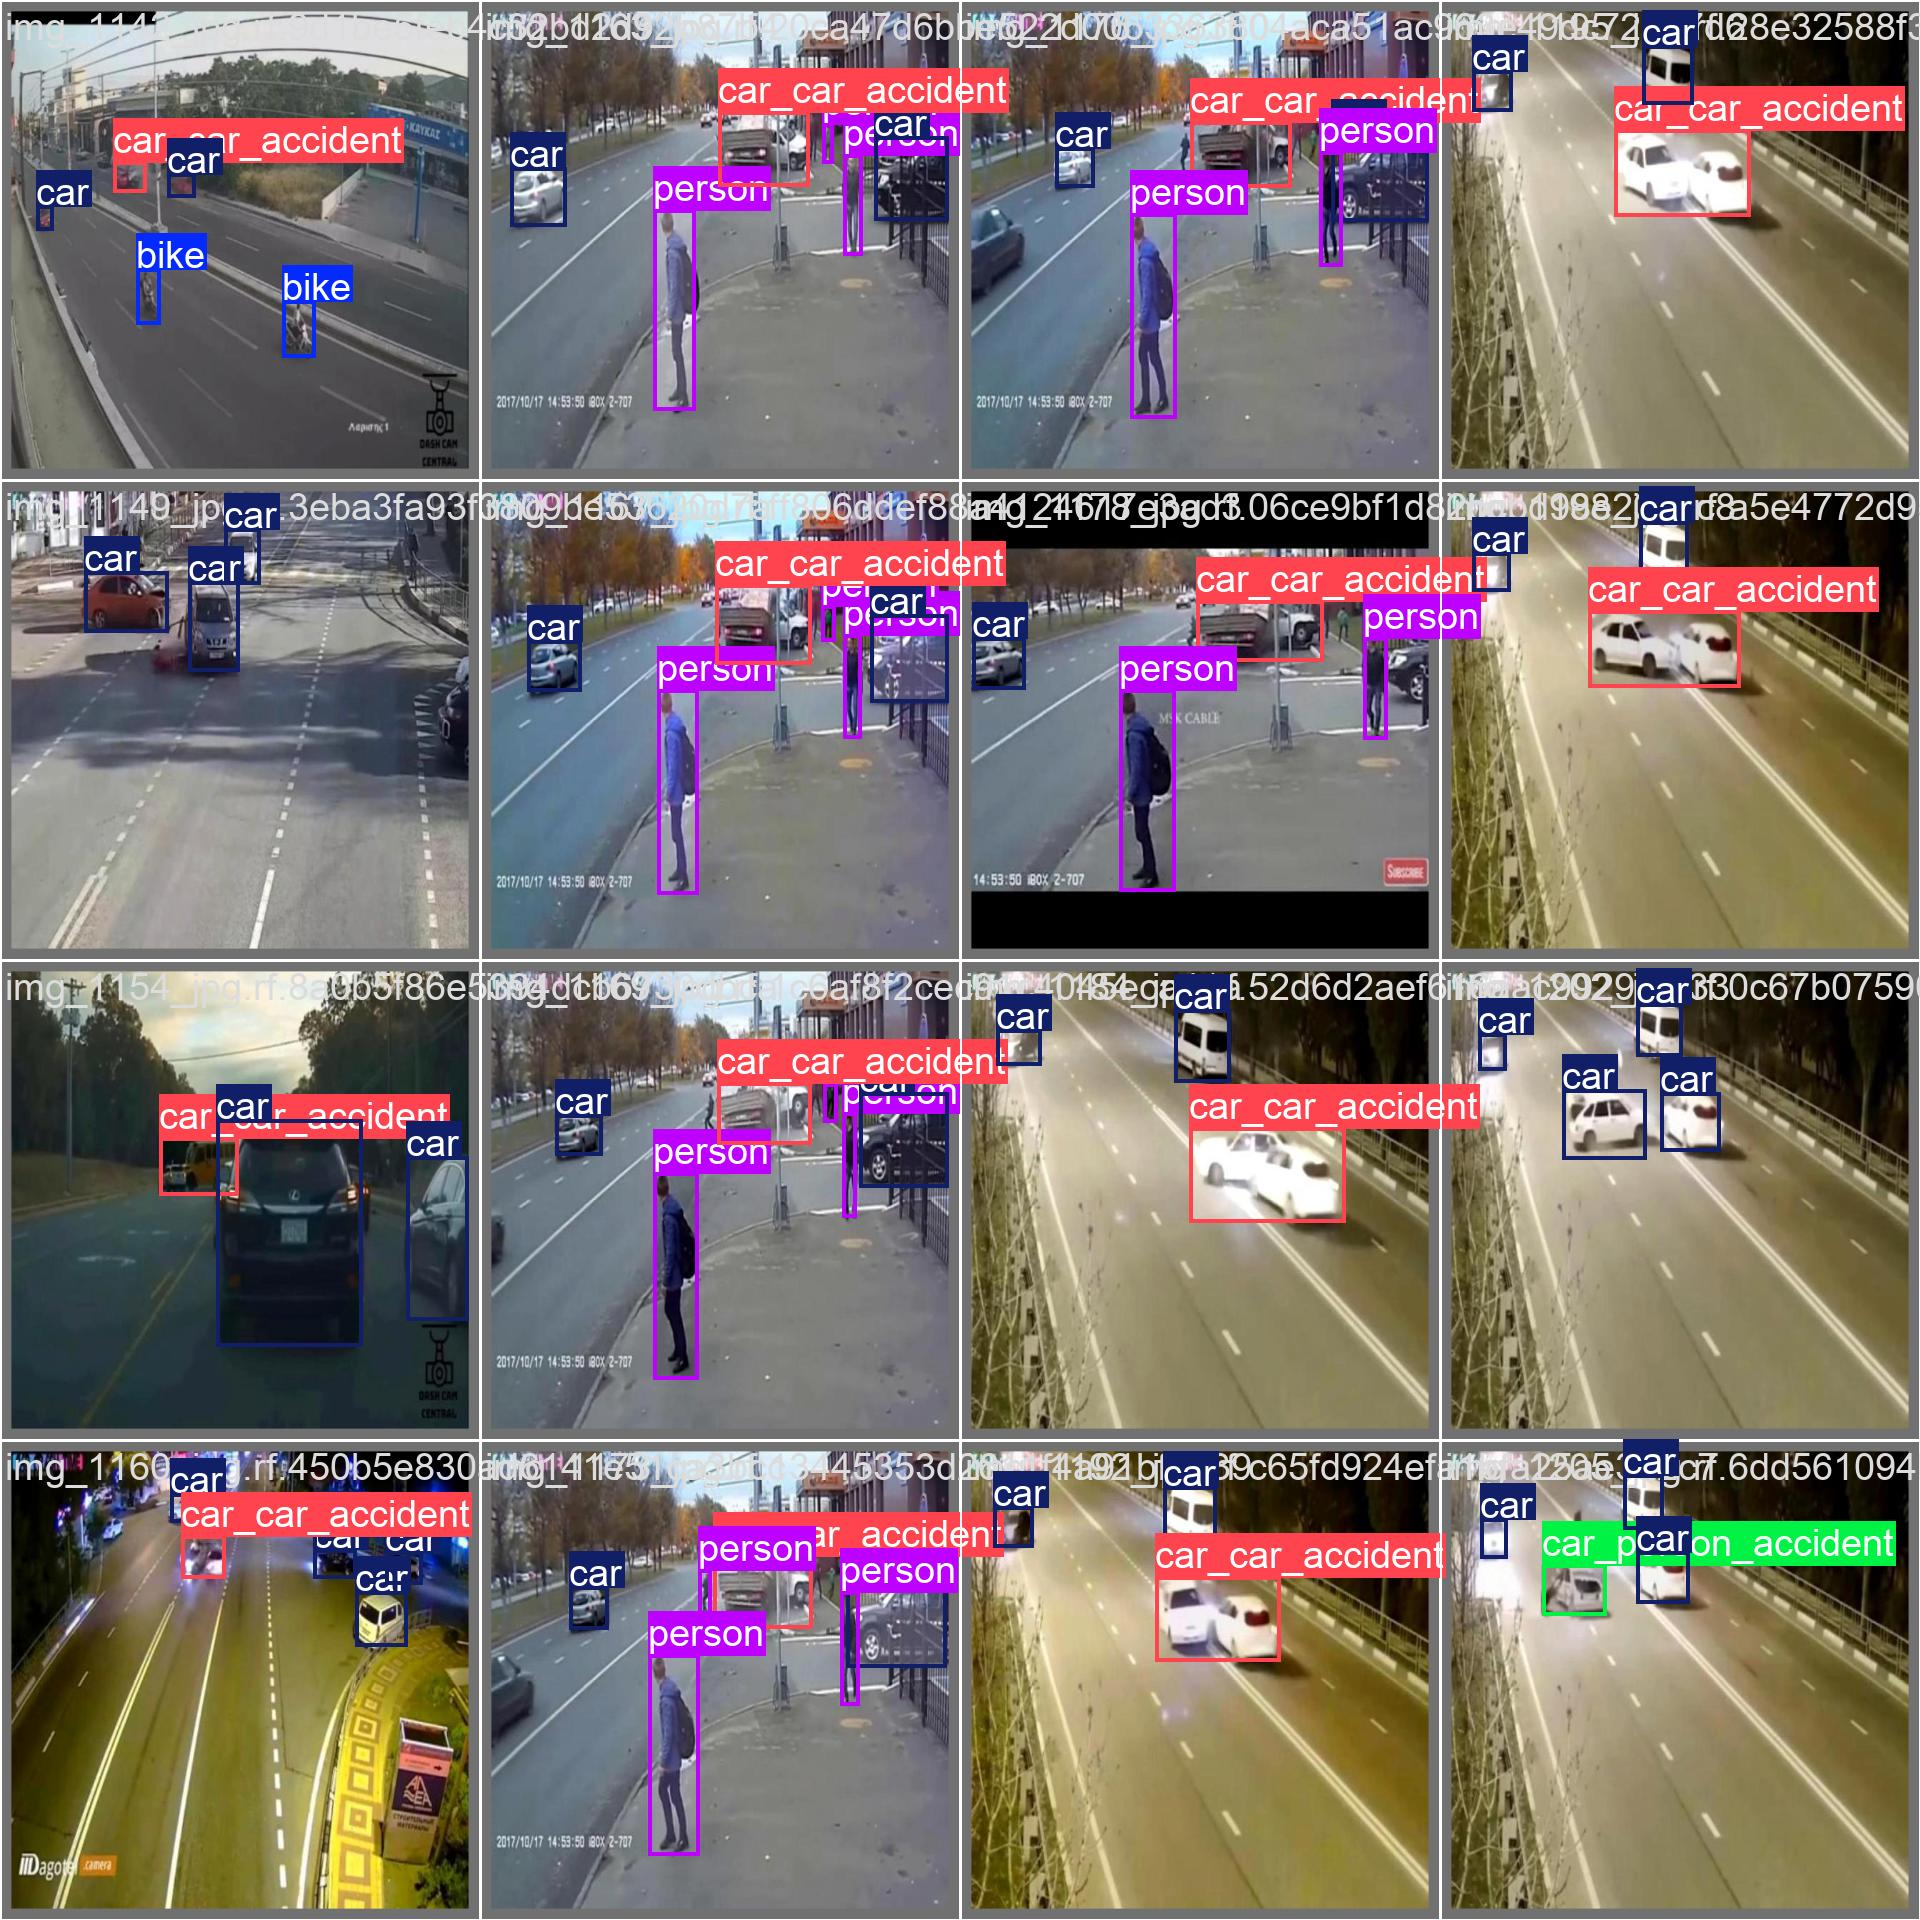
\includegraphics[width=\linewidth]{results/detection/yolo26_baseline/val_batch2_labels.jpg}\end{minipage}
\par\vspace{4pt}
\begin{minipage}{0.32\textwidth}\centering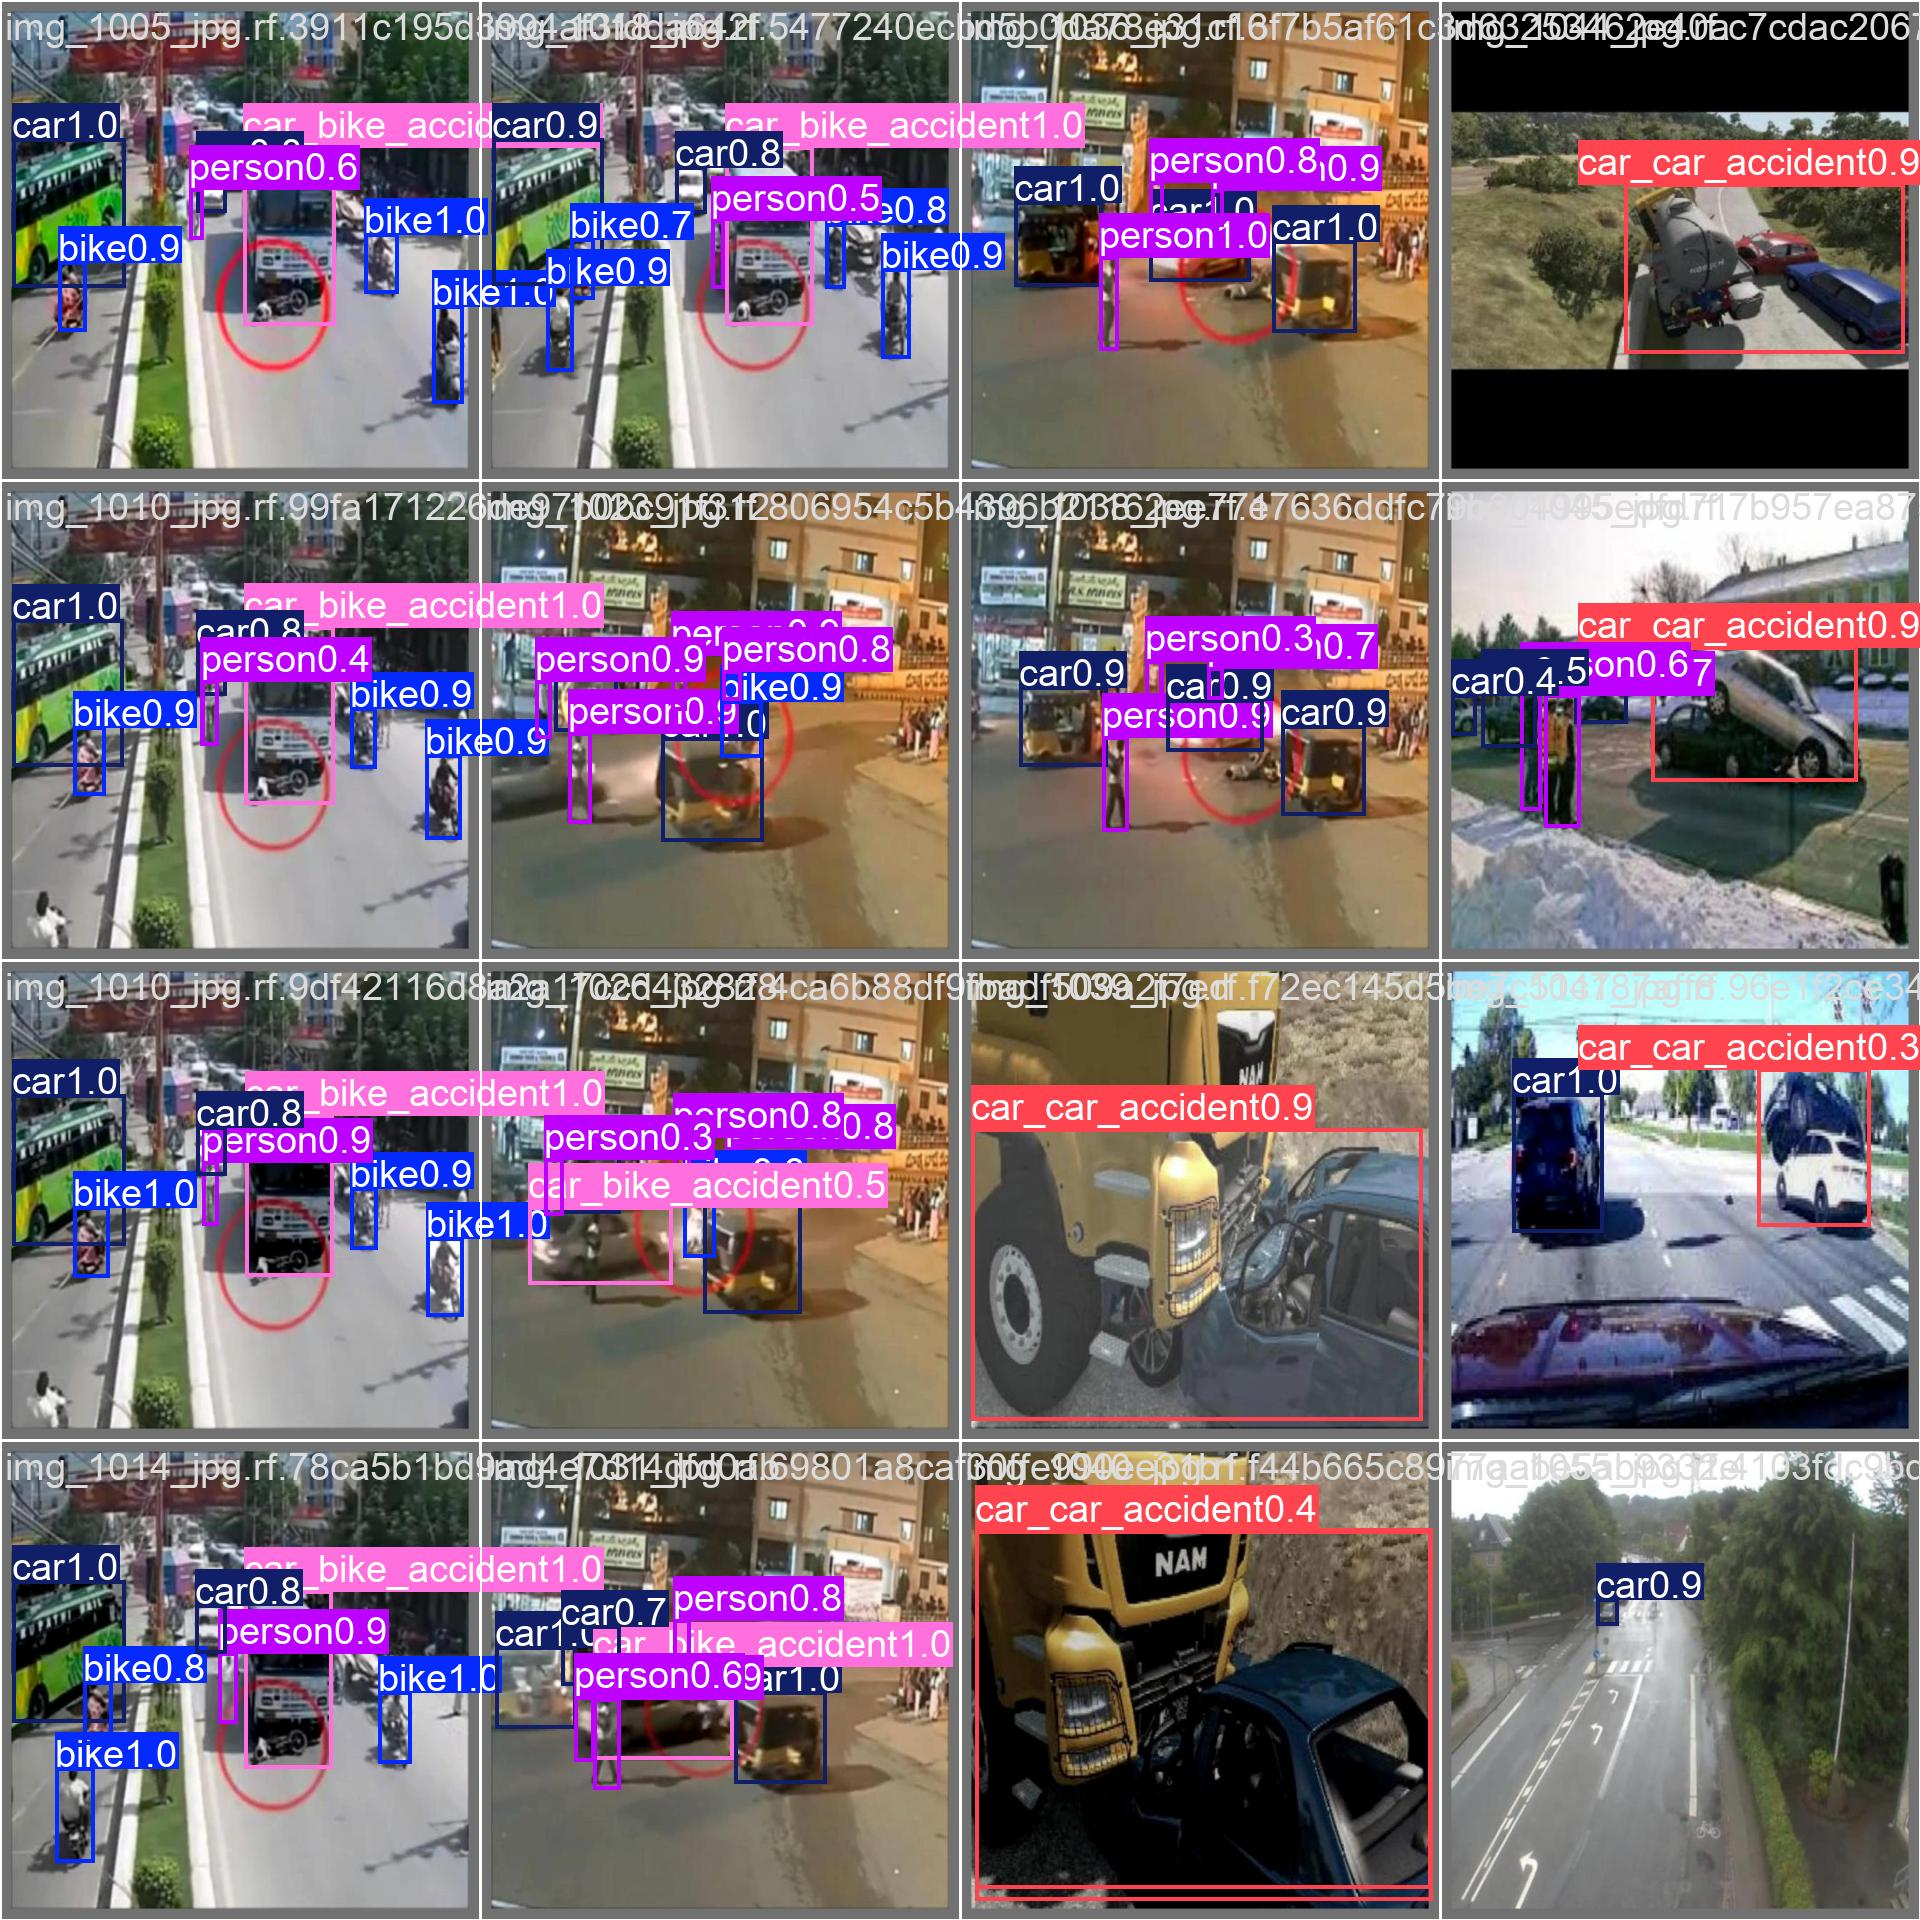
\includegraphics[width=\linewidth]{results/detection/yolo26_baseline/val_batch0_pred.jpg}\end{minipage}
\begin{minipage}{0.32\textwidth}\centering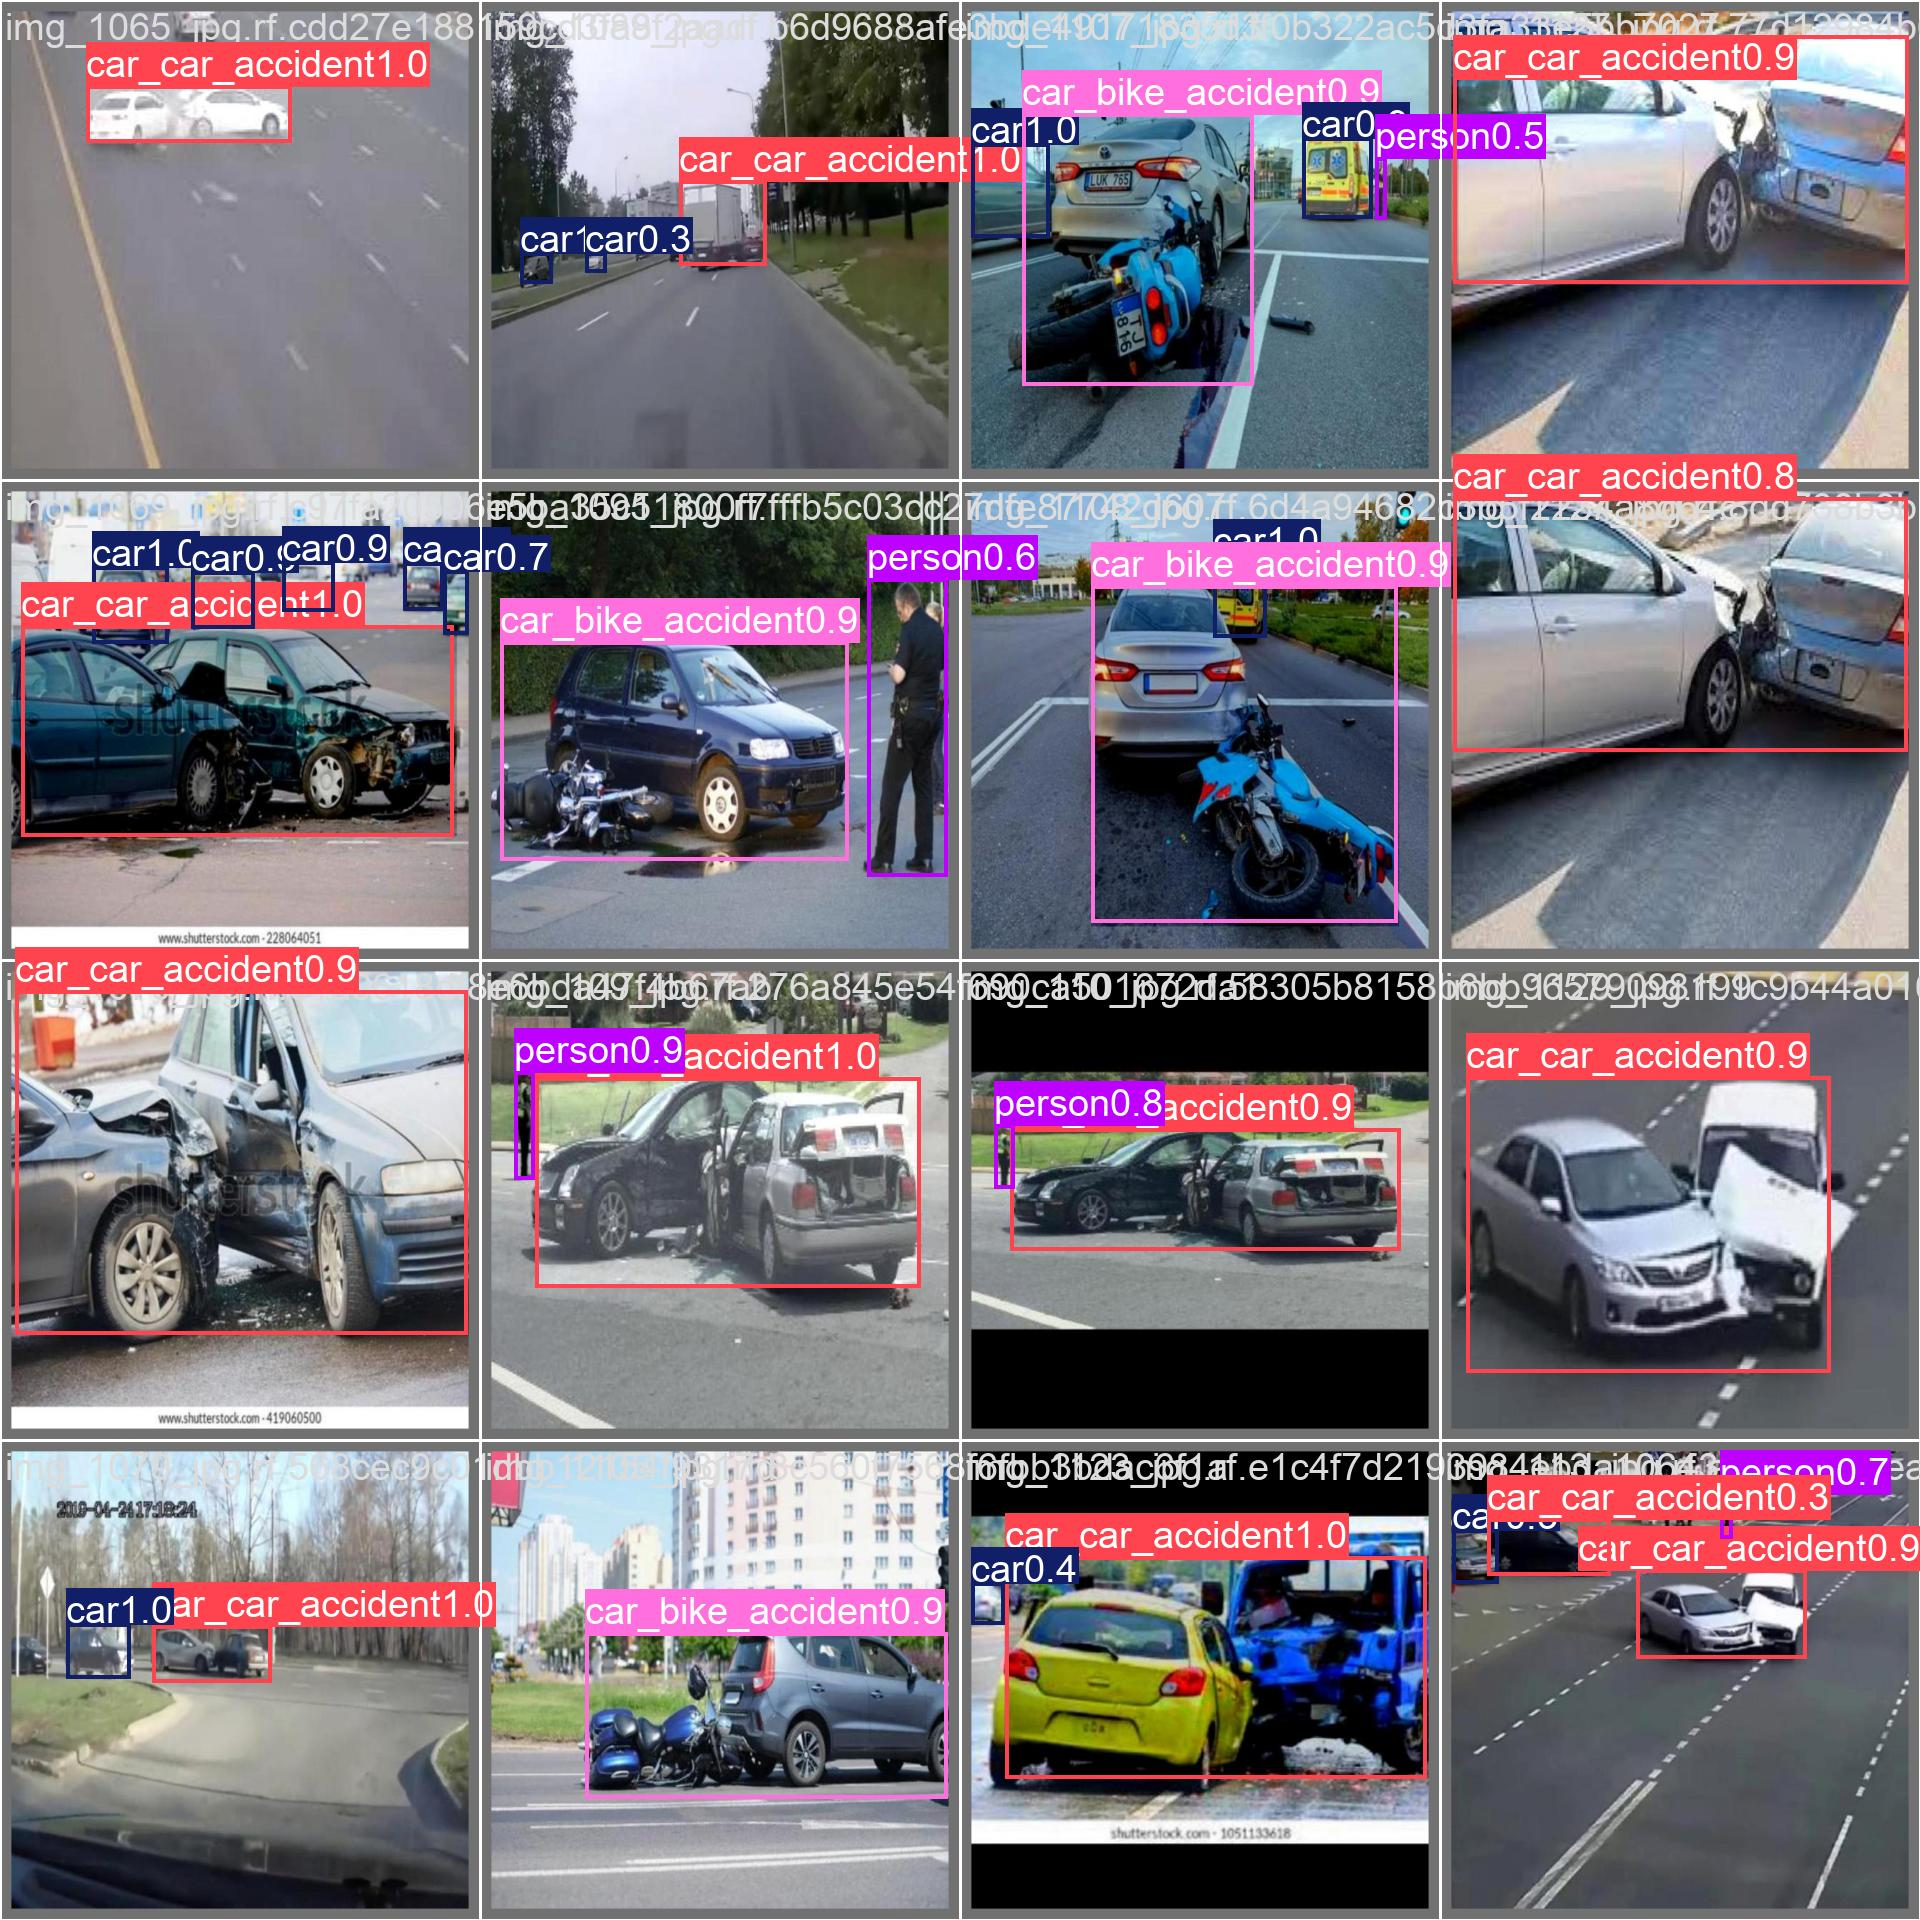
\includegraphics[width=\linewidth]{results/detection/yolo26_baseline/val_batch1_pred.jpg}\end{minipage}
\begin{minipage}{0.32\textwidth}\centering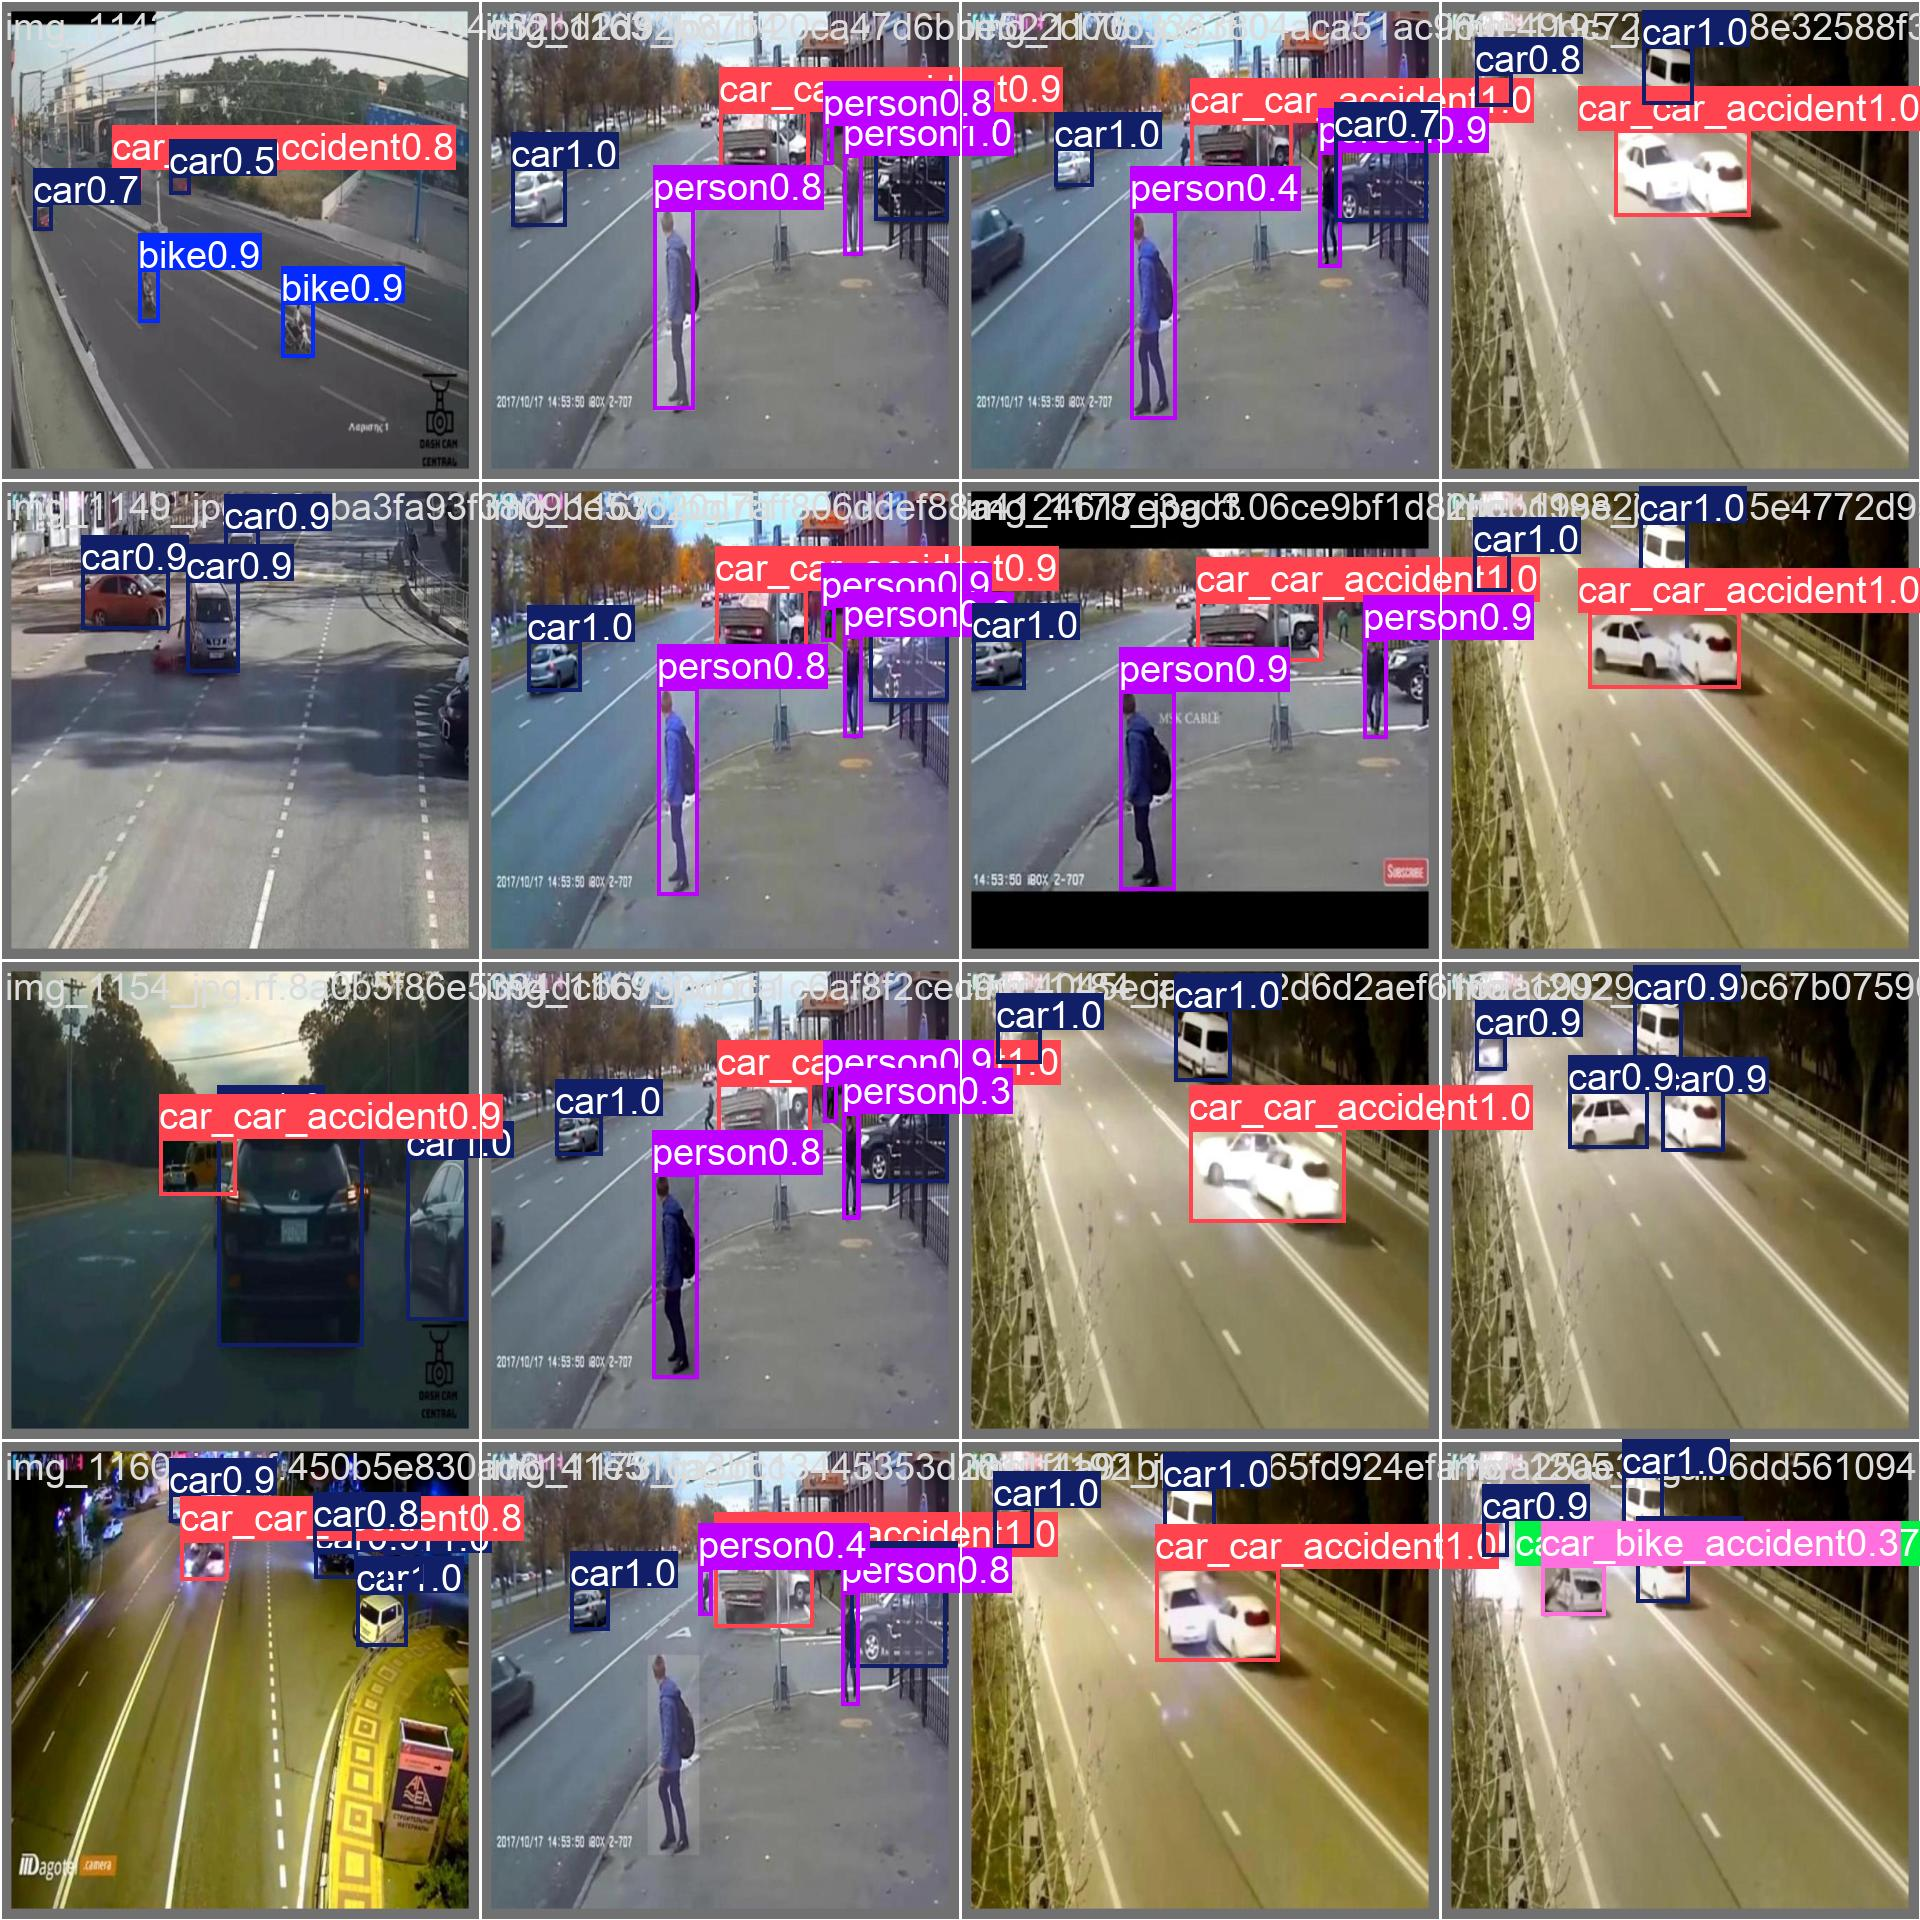
\includegraphics[width=\linewidth]{results/detection/yolo26_baseline/val_batch2_pred.jpg}\end{minipage}
\caption{All saved validation batches for Accident Detection: ground-truth labels above and predictions below.}
\end{figure}
\section{Accident Severity Training and Validation Previews}
\begin{figure}[t]\centering
\begin{minipage}{0.32\textwidth}\centering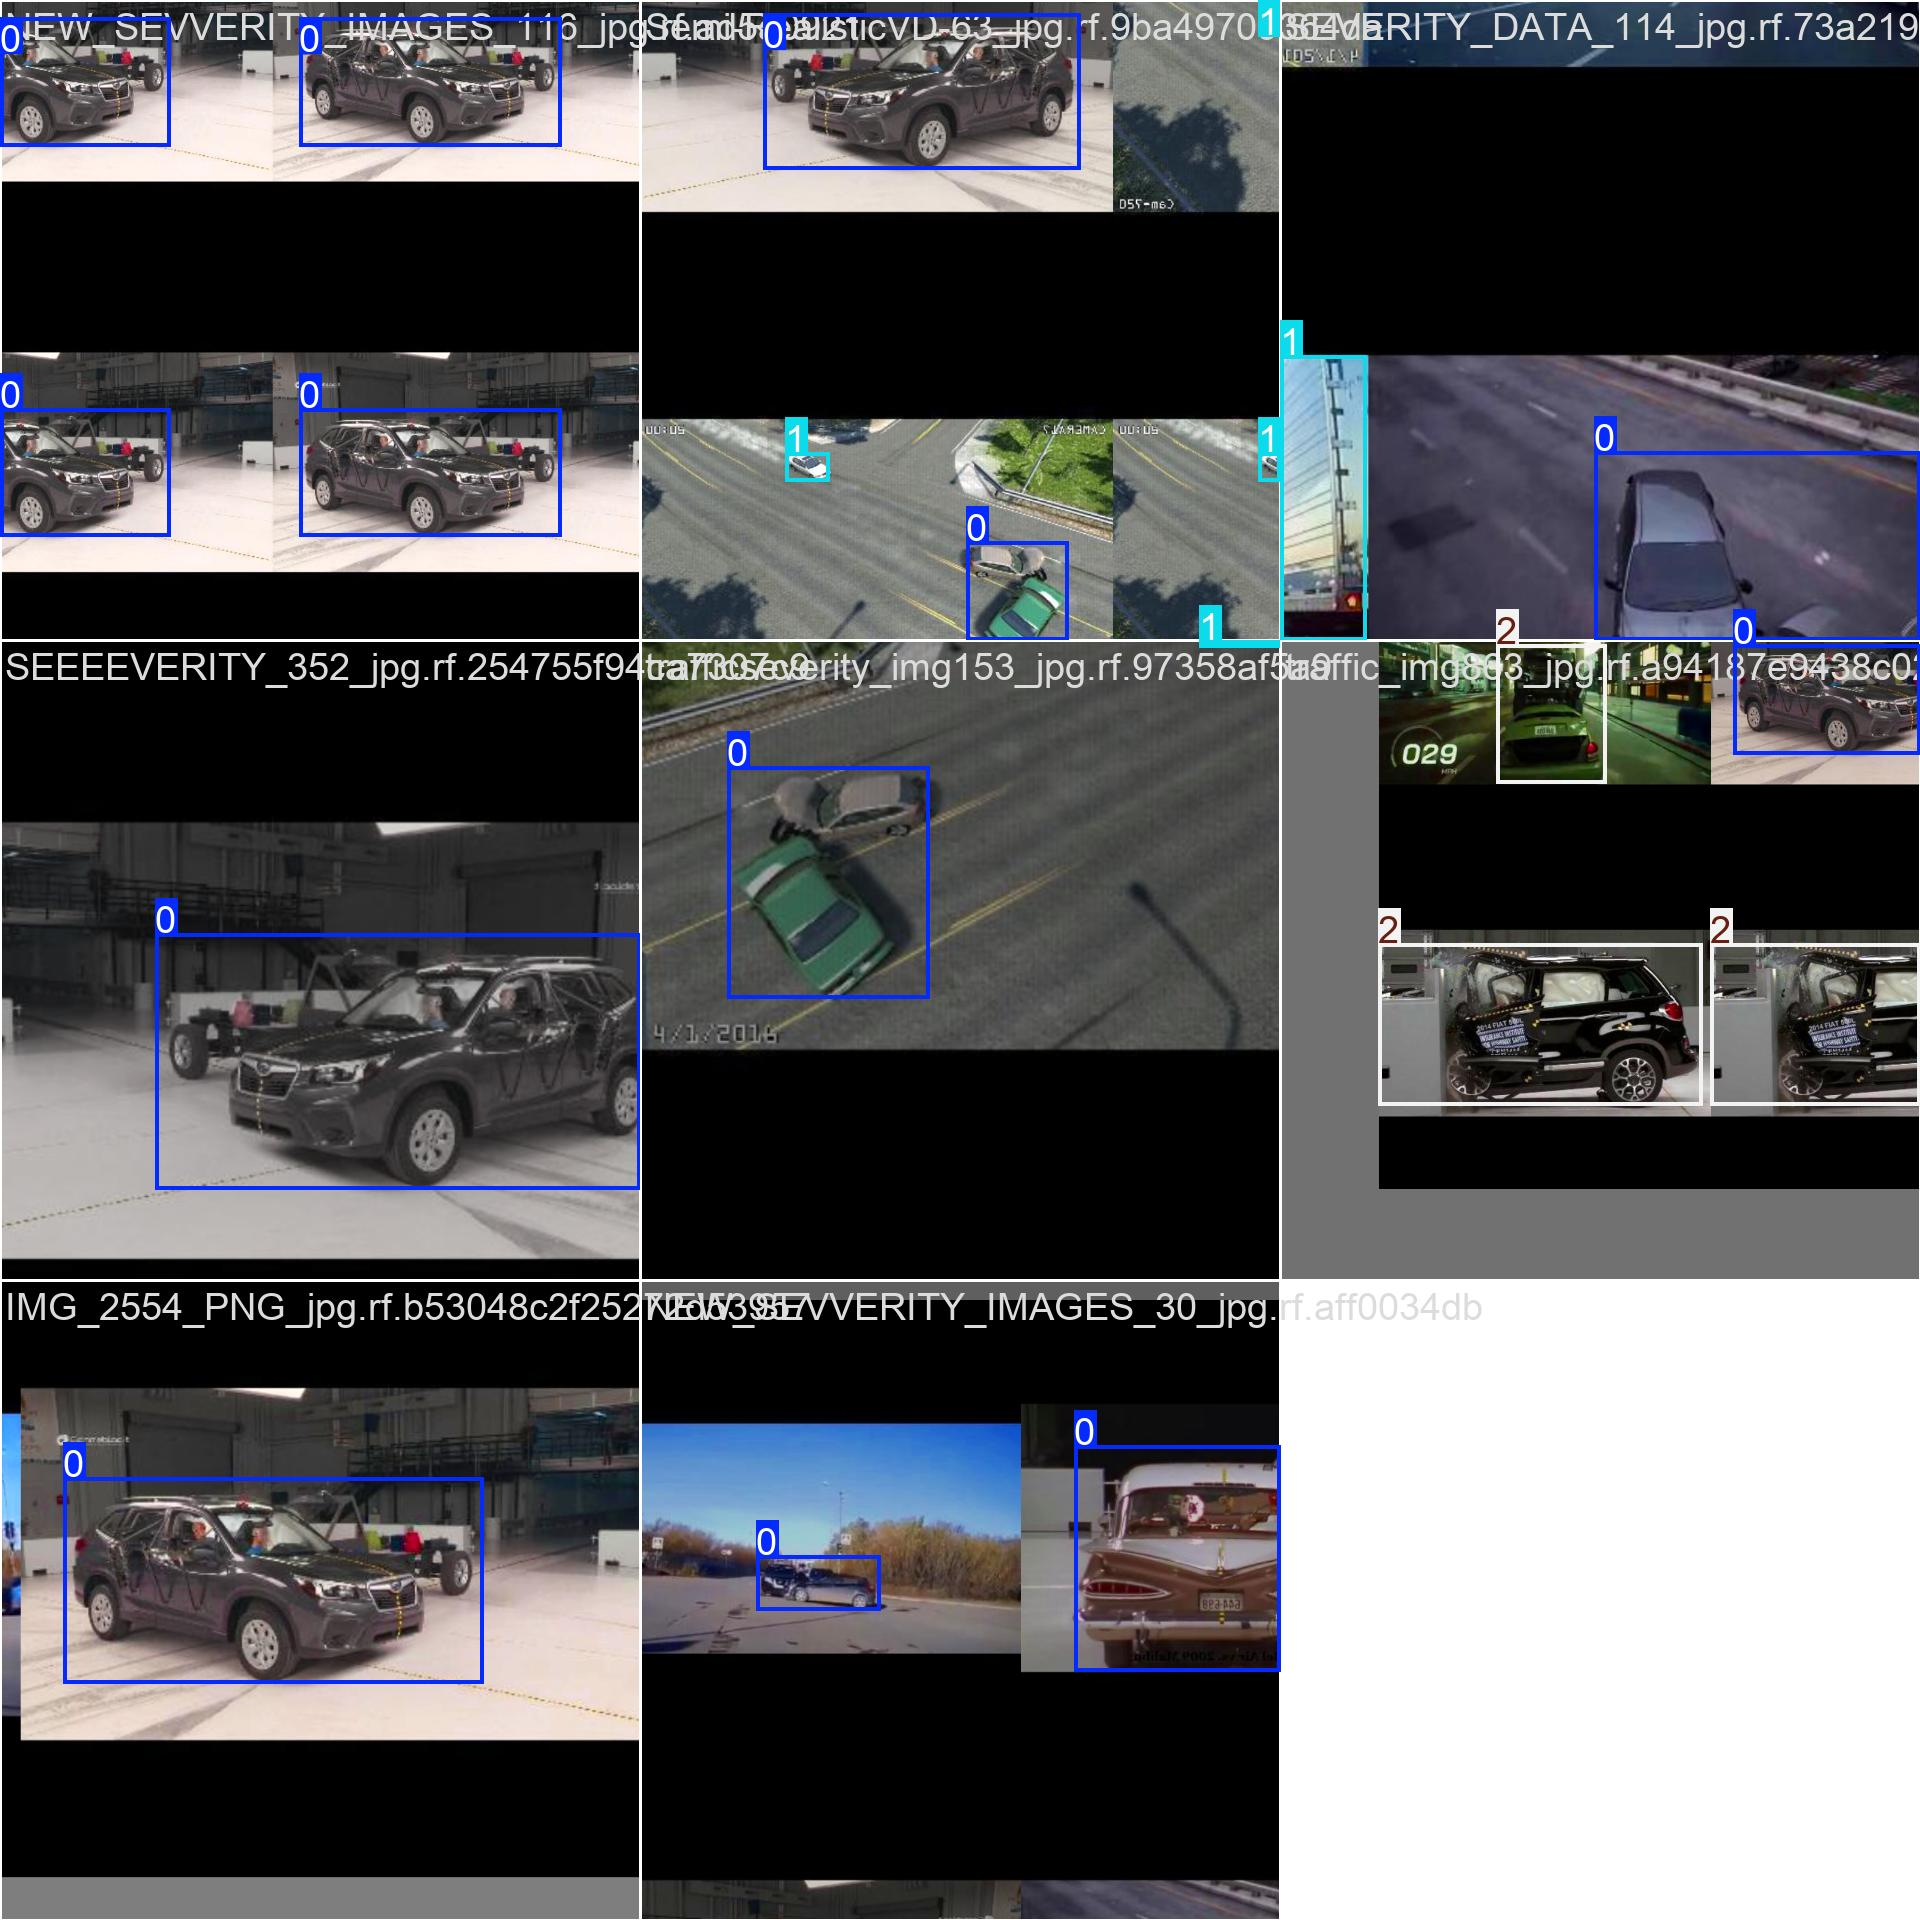
\includegraphics[width=\linewidth]{results/detection/accident_severity-2/train_batch0.jpg}\end{minipage}
\begin{minipage}{0.32\textwidth}\centering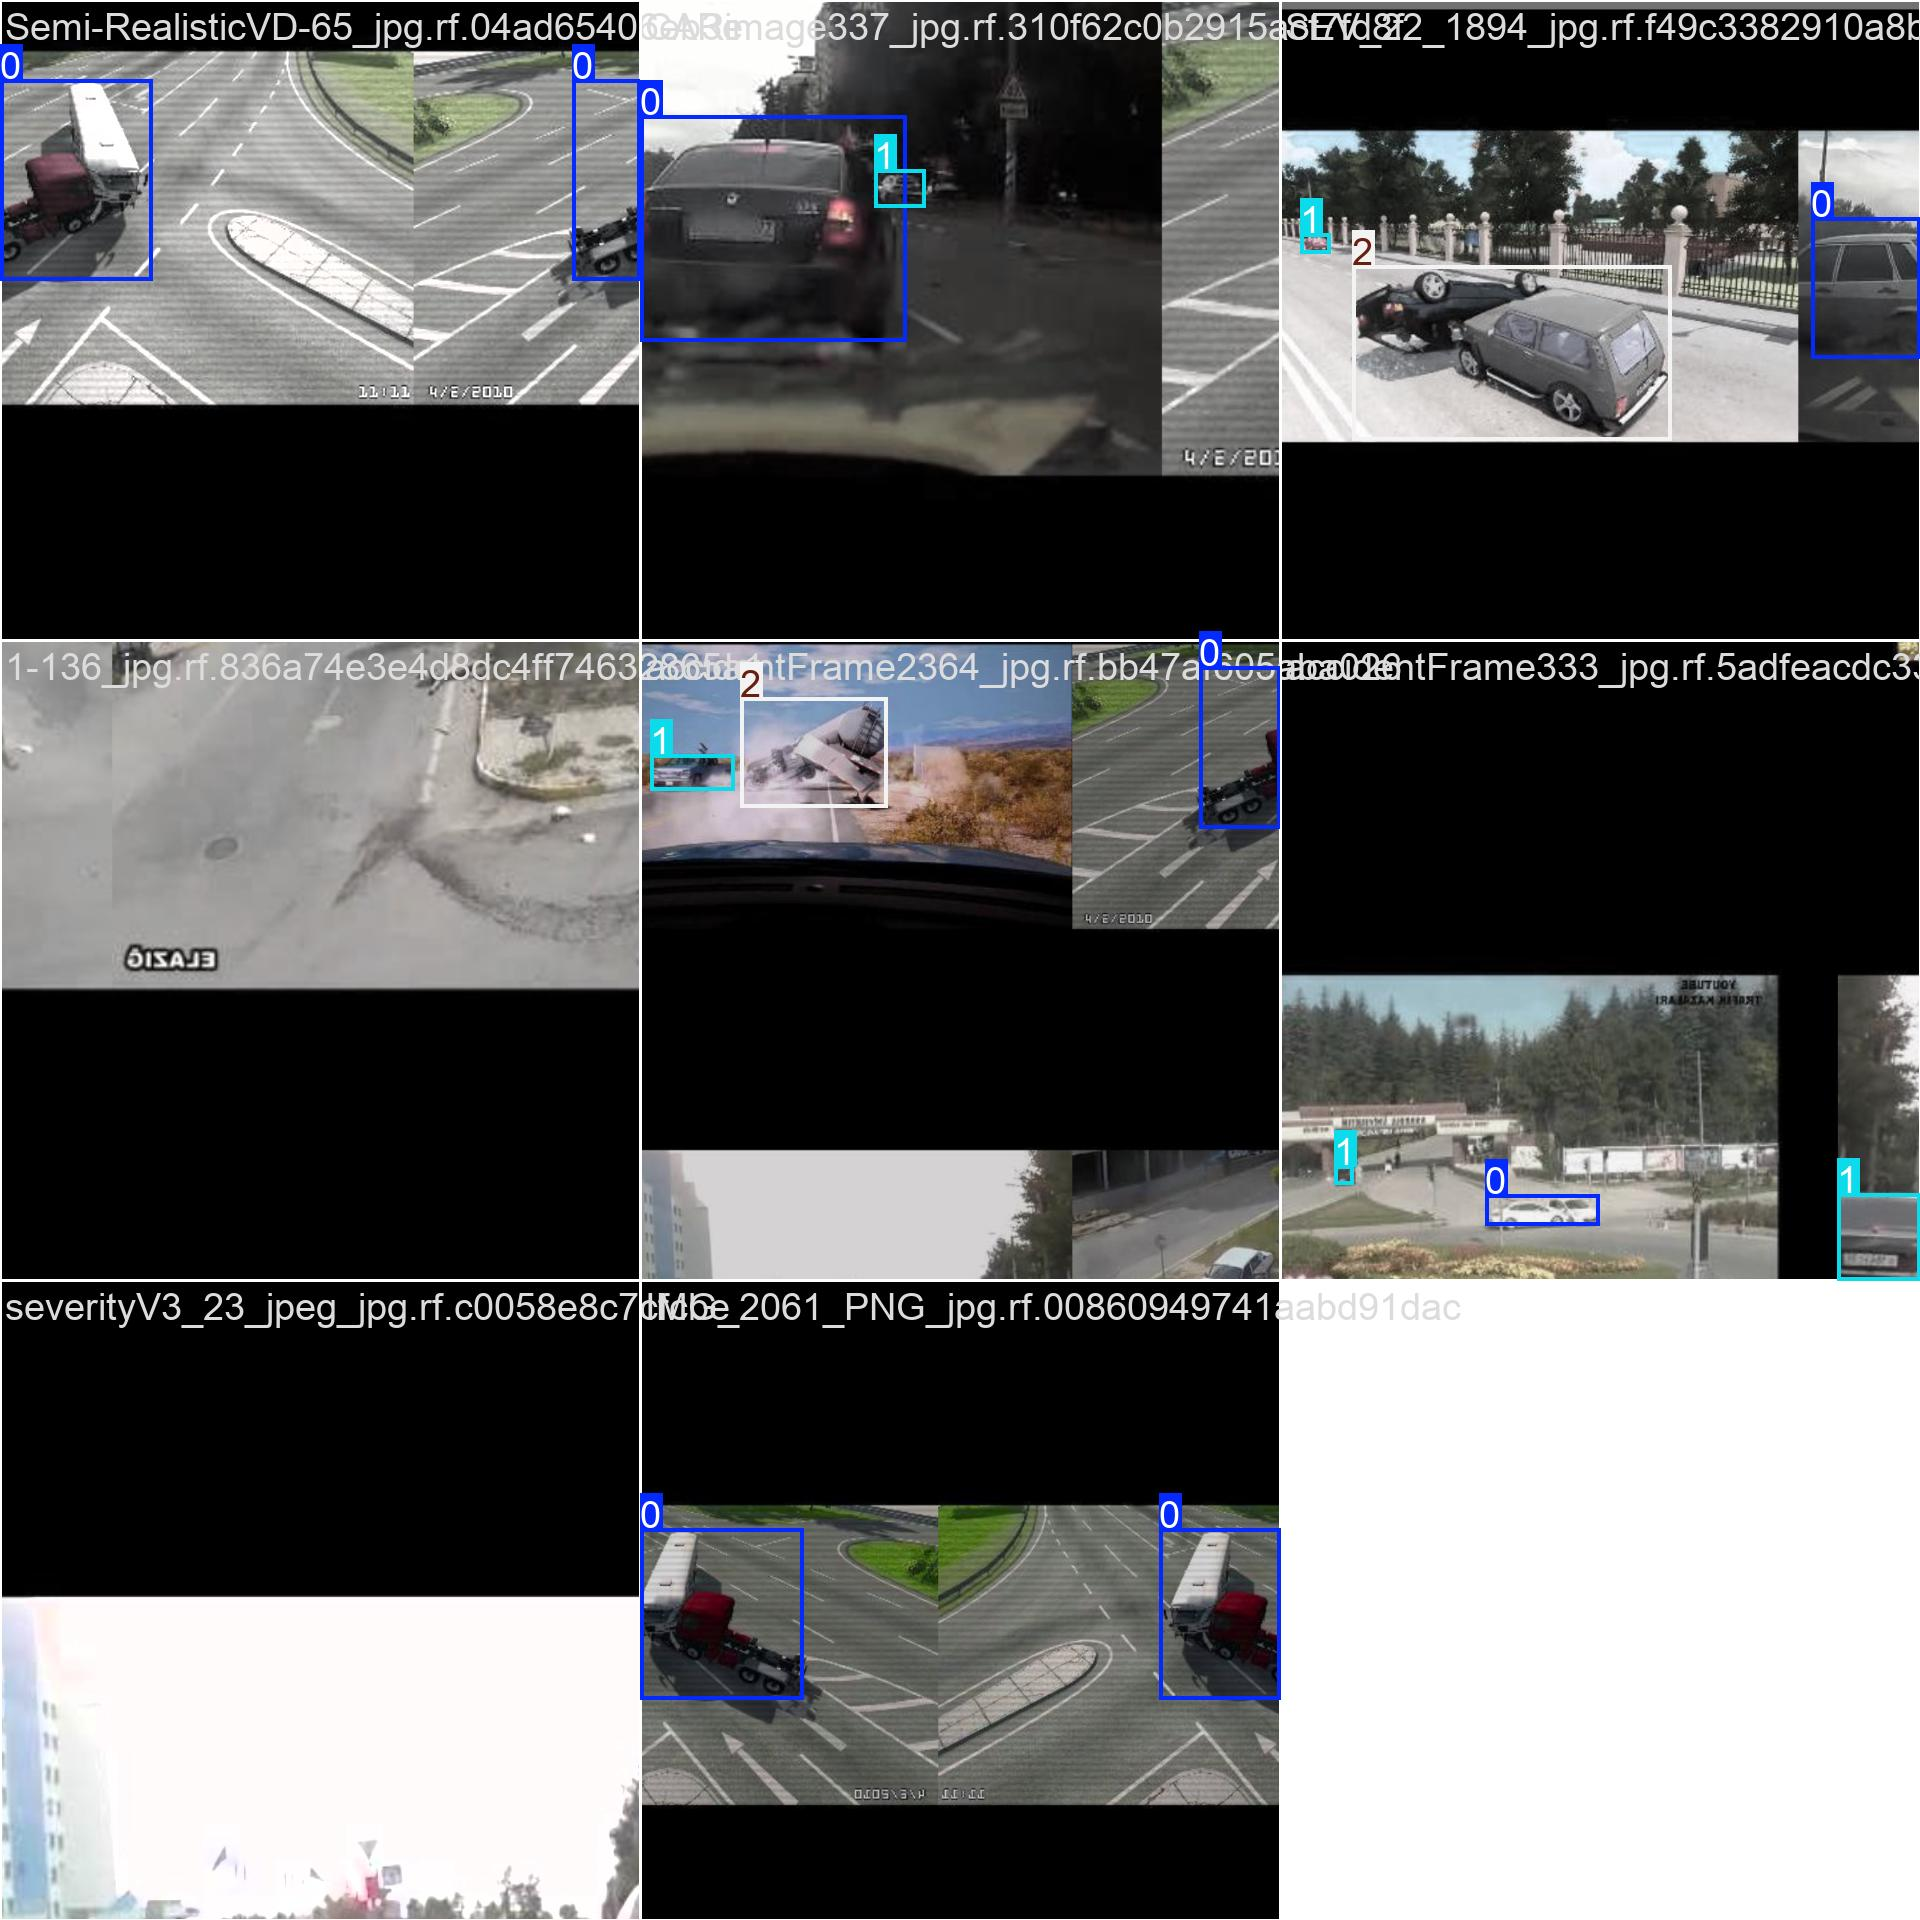
\includegraphics[width=\linewidth]{results/detection/accident_severity-2/train_batch1.jpg}\end{minipage}
\begin{minipage}{0.32\textwidth}\centering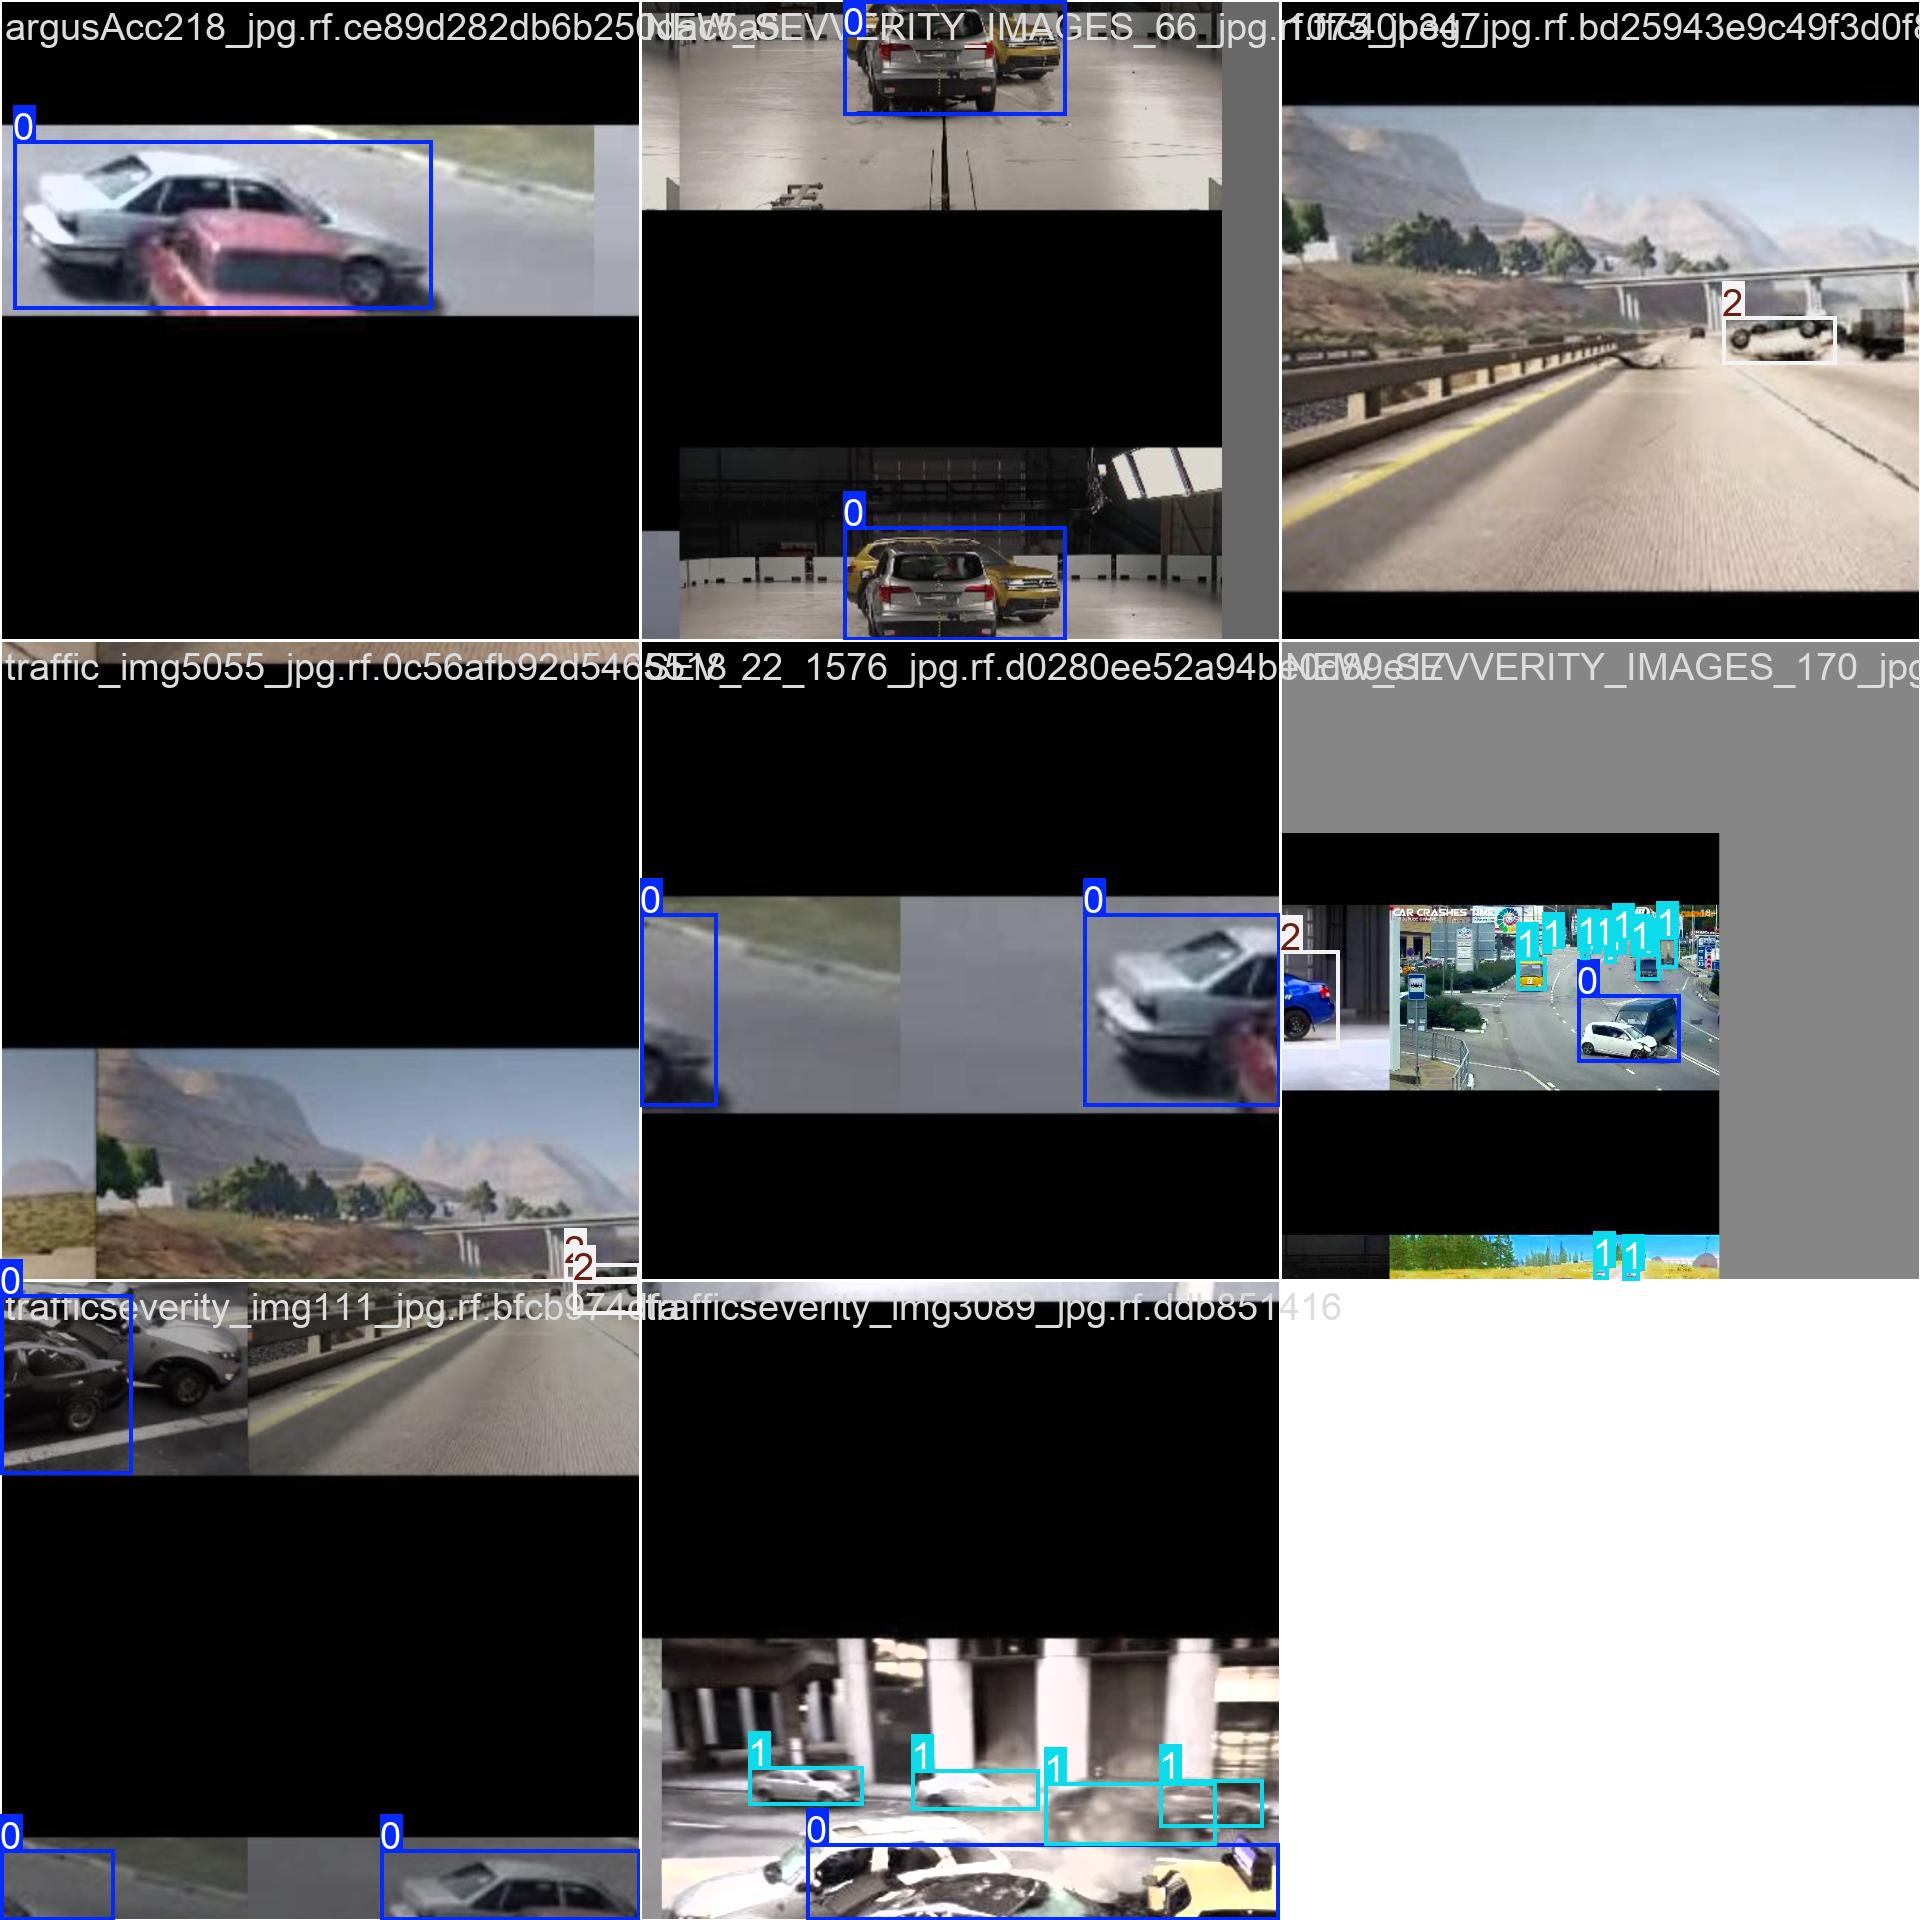
\includegraphics[width=\linewidth]{results/detection/accident_severity-2/train_batch2.jpg}\end{minipage}
\caption{Saved training-batch previews for Accident Severity.}
\end{figure}
\begin{figure}[t]\centering
\begin{minipage}{0.32\textwidth}\centering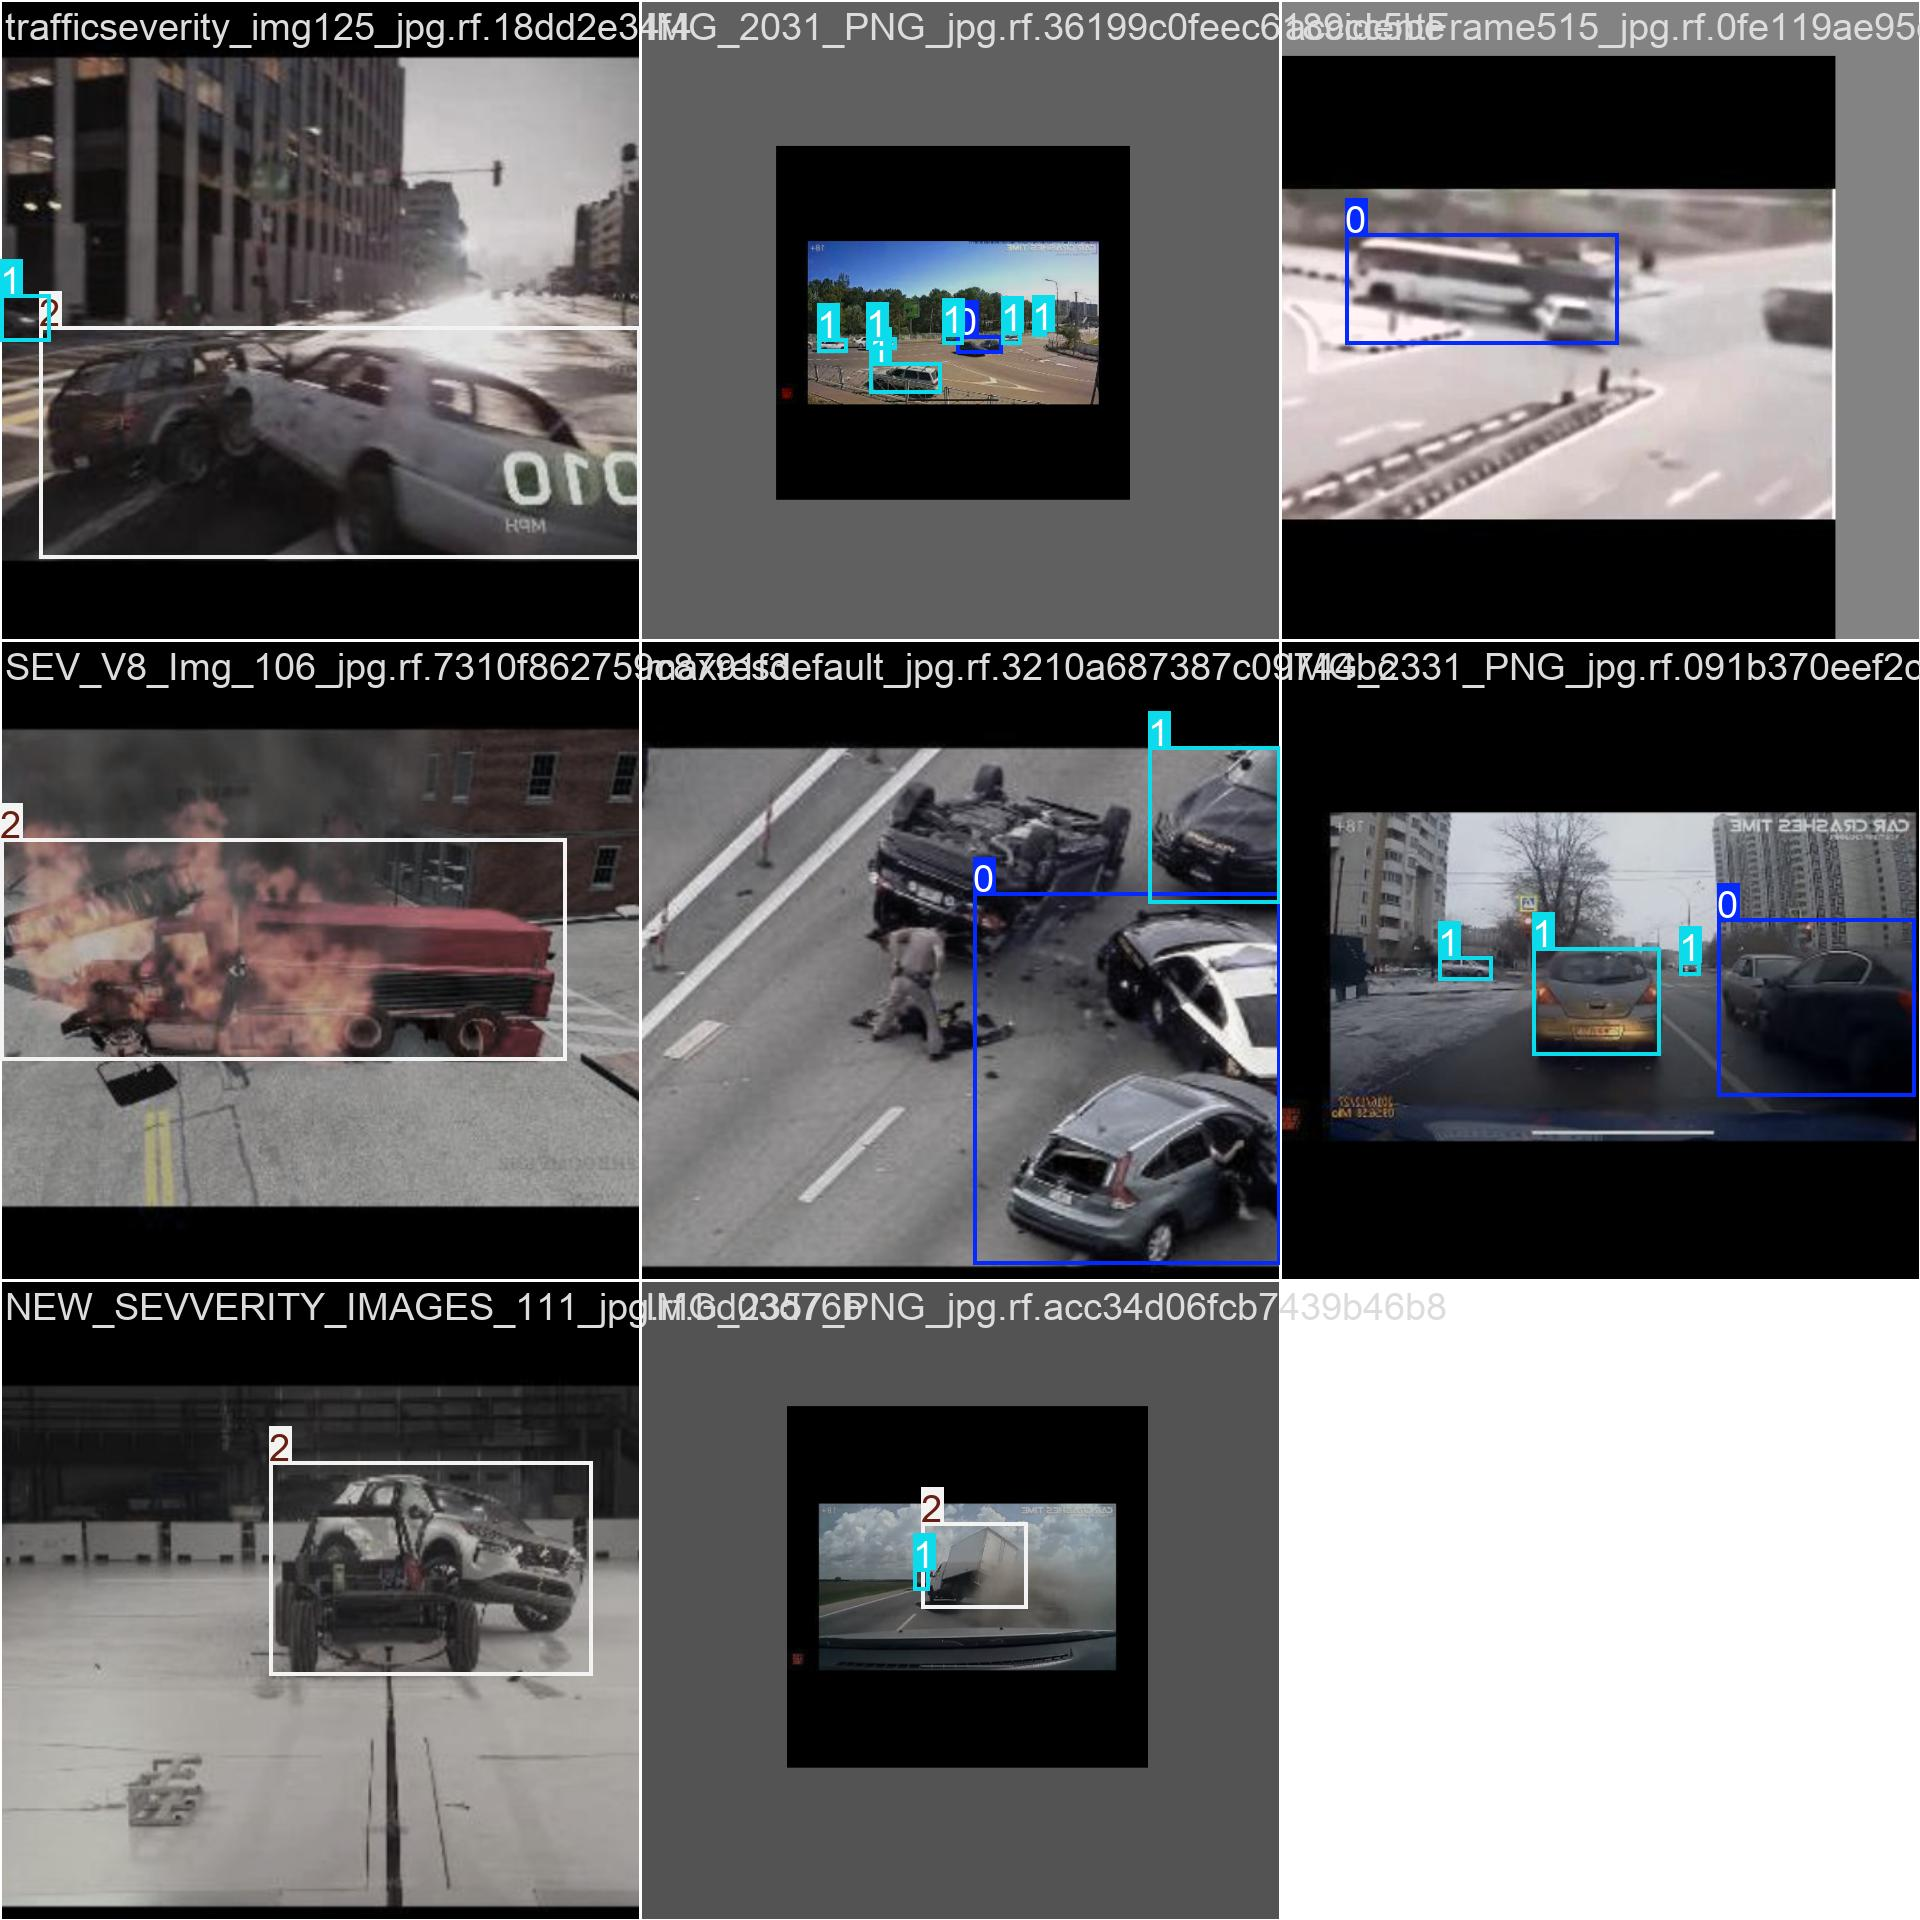
\includegraphics[width=\linewidth]{results/detection/accident_severity-2/train_batch40050.jpg}\end{minipage}
\begin{minipage}{0.32\textwidth}\centering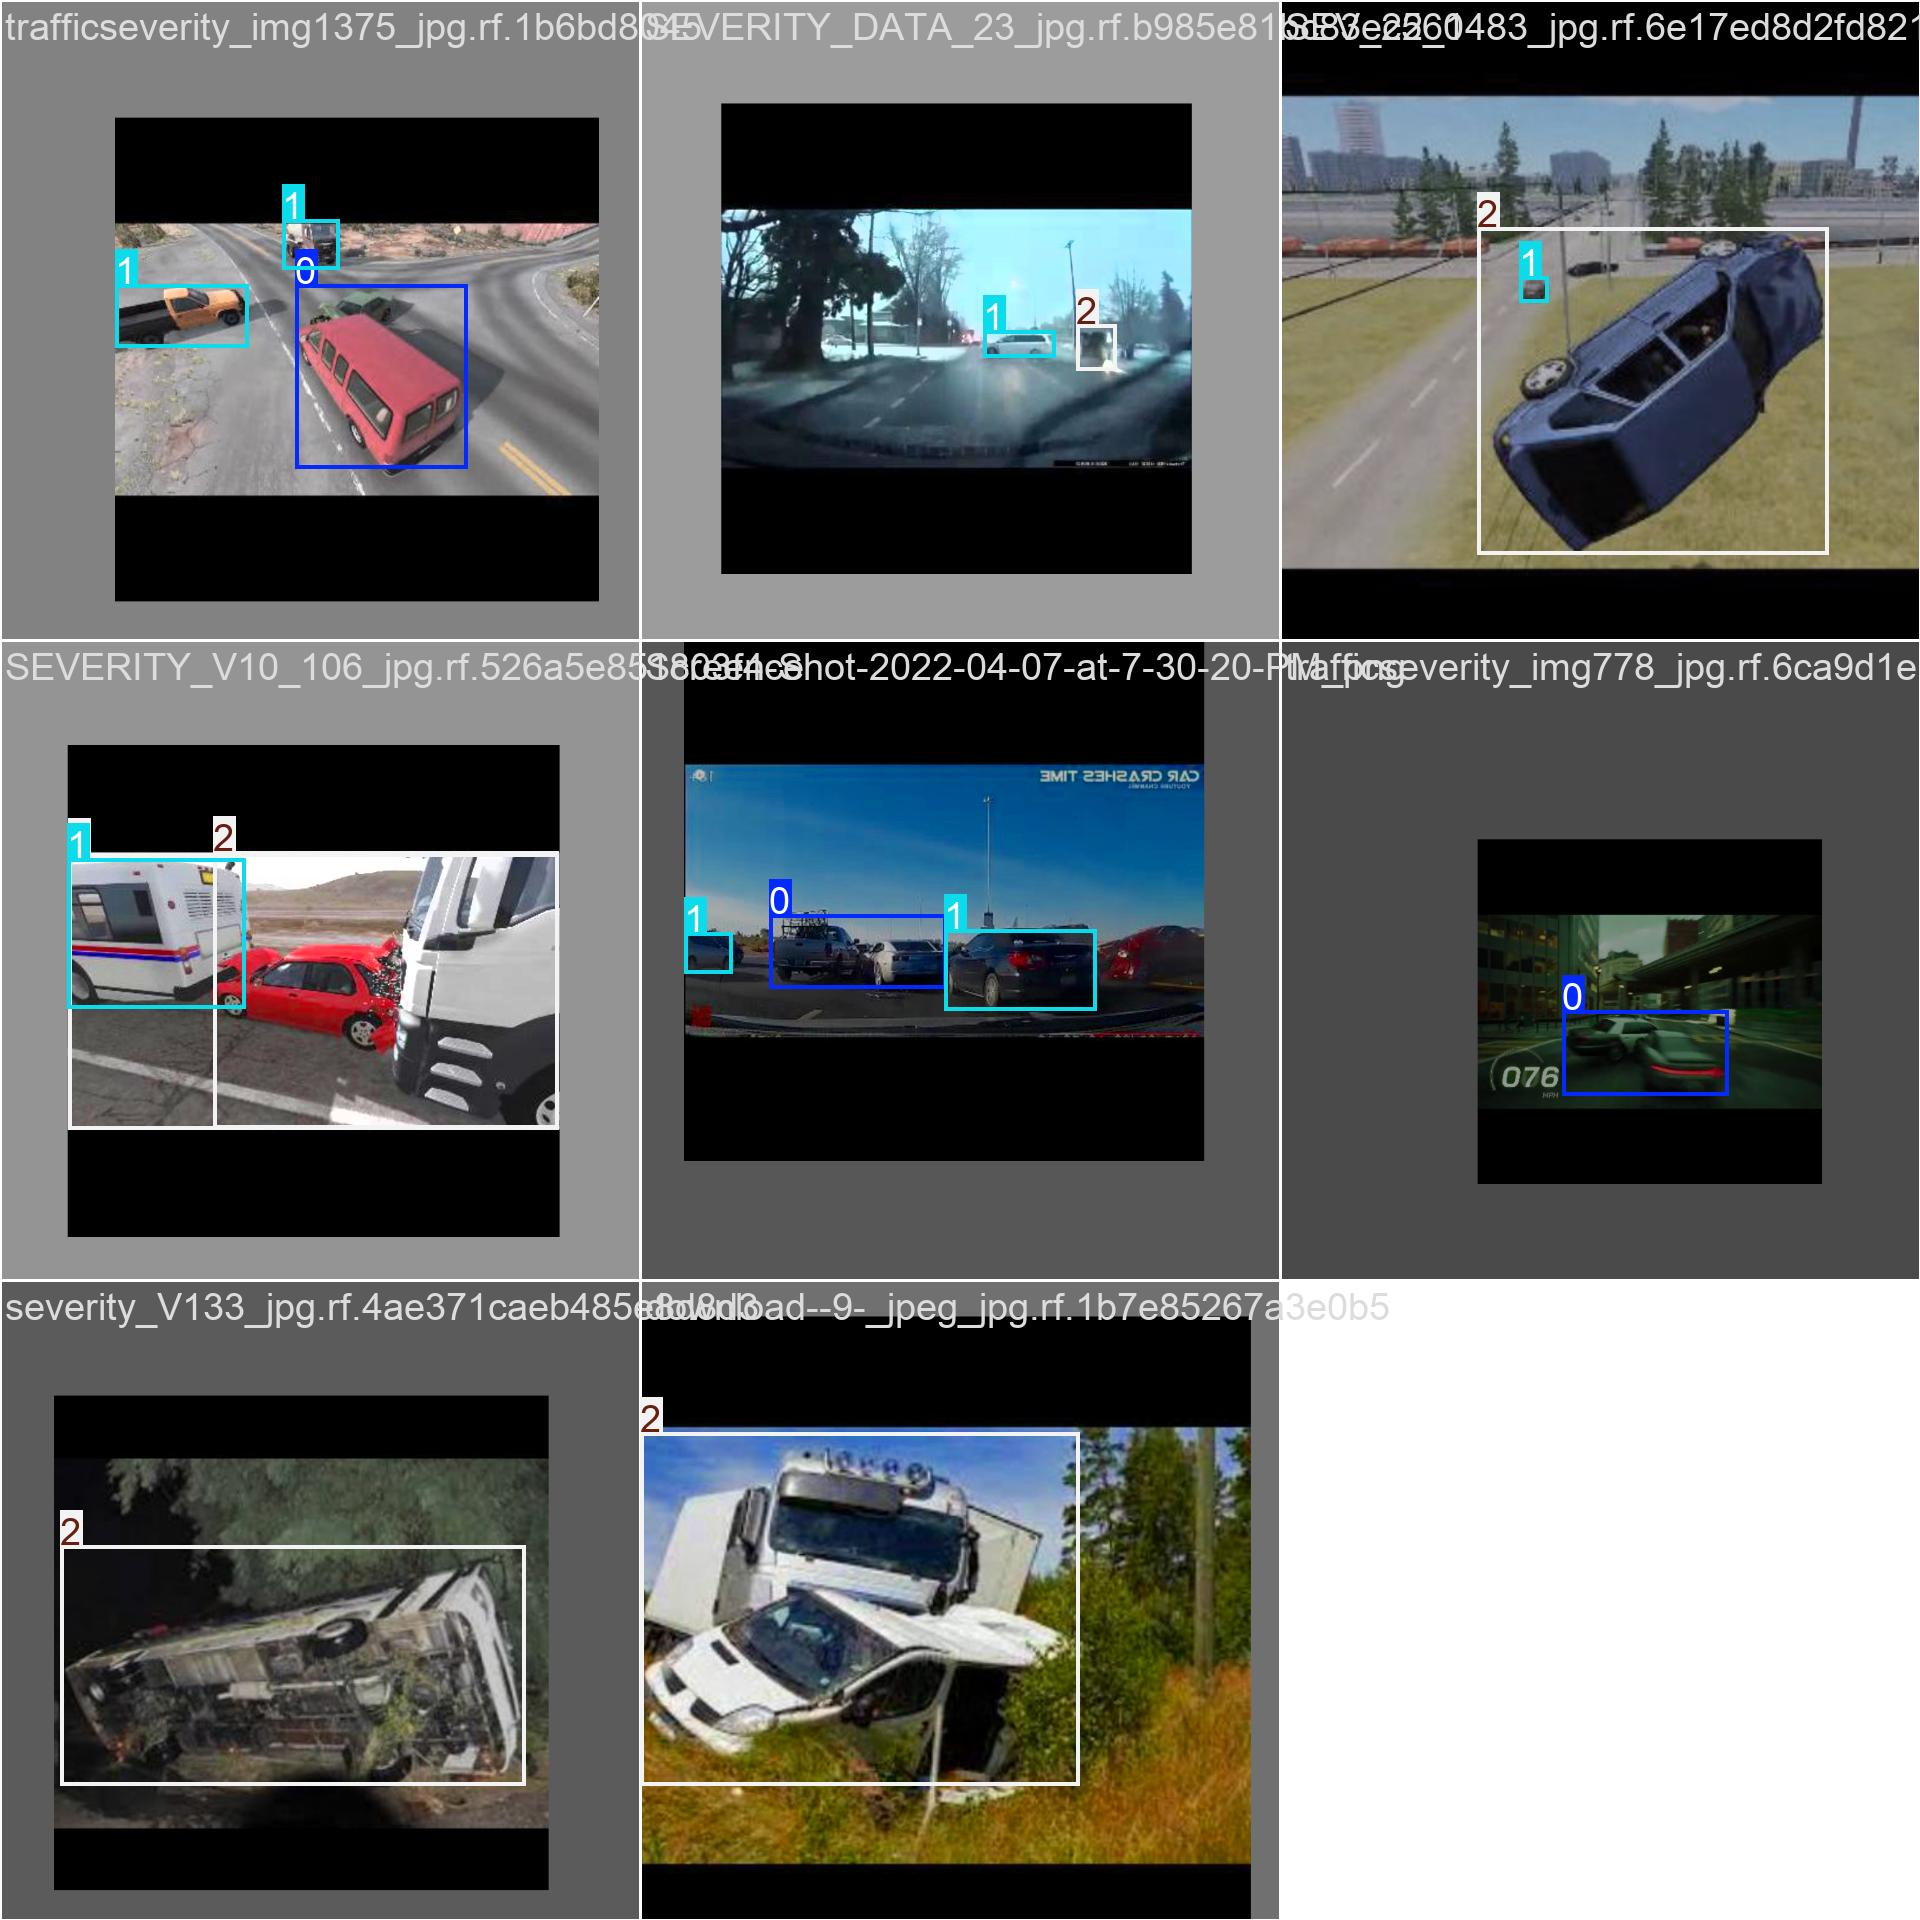
\includegraphics[width=\linewidth]{results/detection/accident_severity-2/train_batch40051.jpg}\end{minipage}
\begin{minipage}{0.32\textwidth}\centering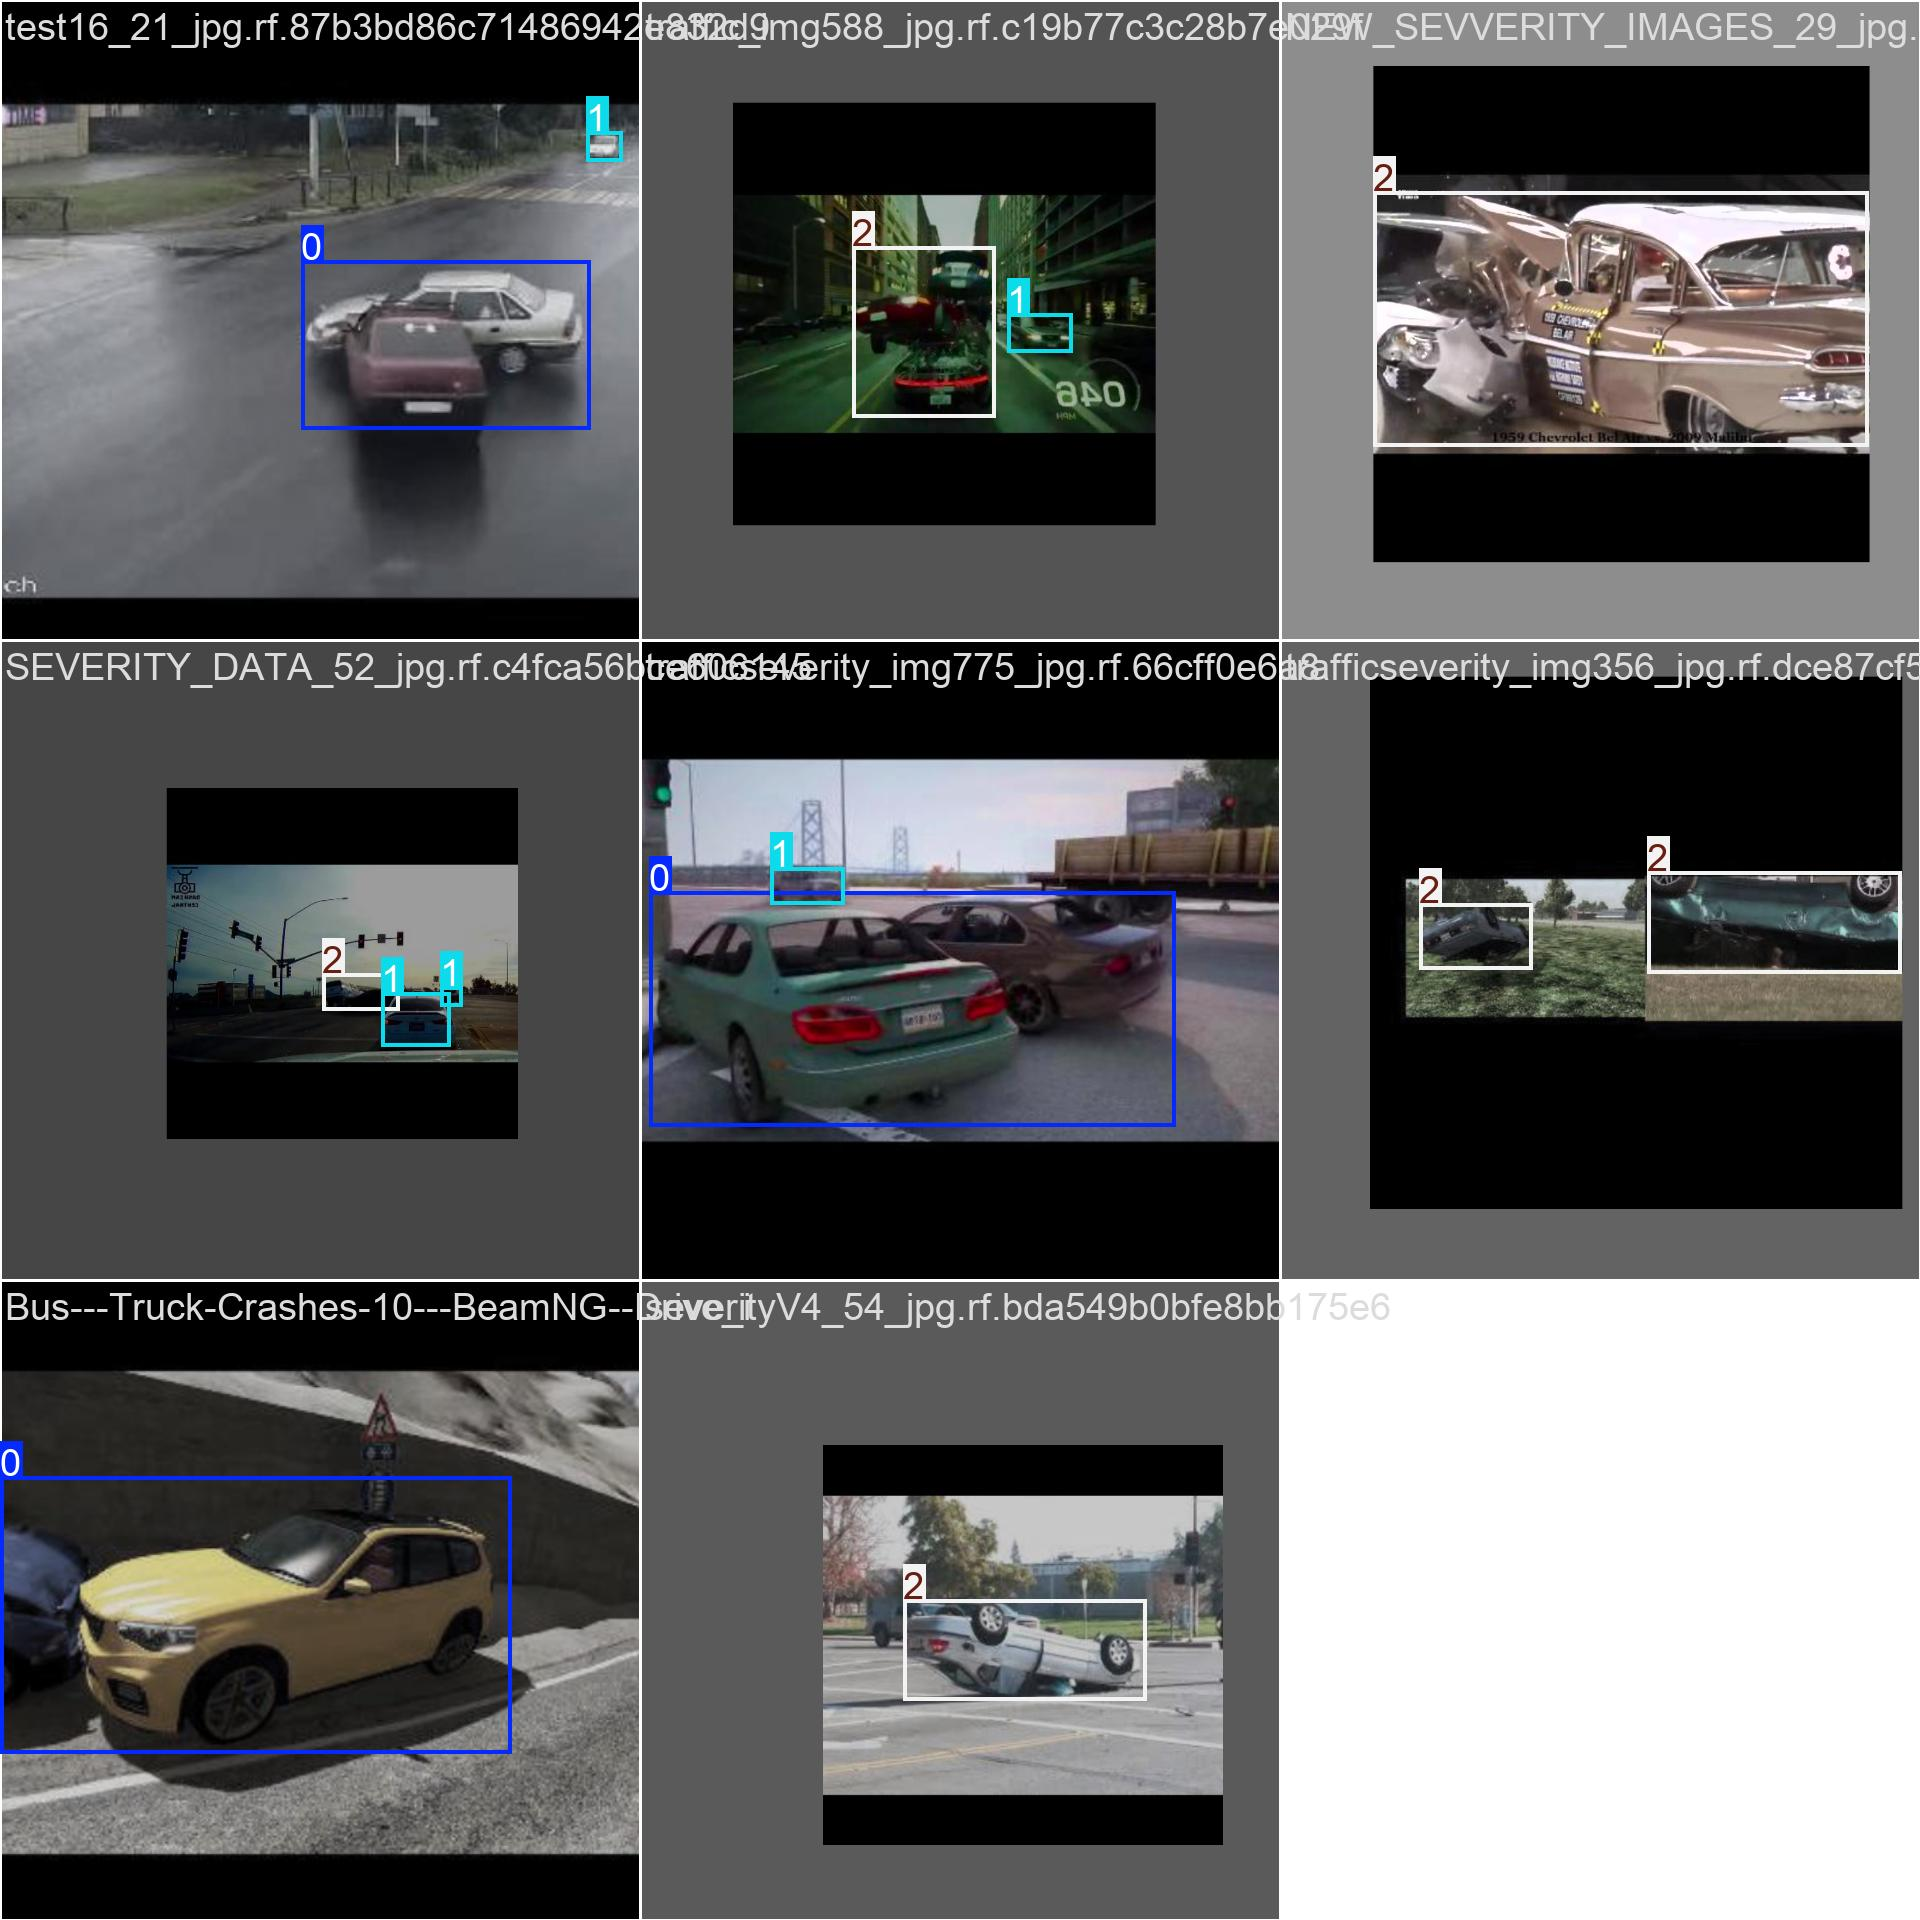
\includegraphics[width=\linewidth]{results/detection/accident_severity-2/train_batch40052.jpg}\end{minipage}
\caption{Saved training-batch previews for Accident Severity.}
\end{figure}
\begin{figure}[t]\centering
\begin{minipage}{0.32\textwidth}\centering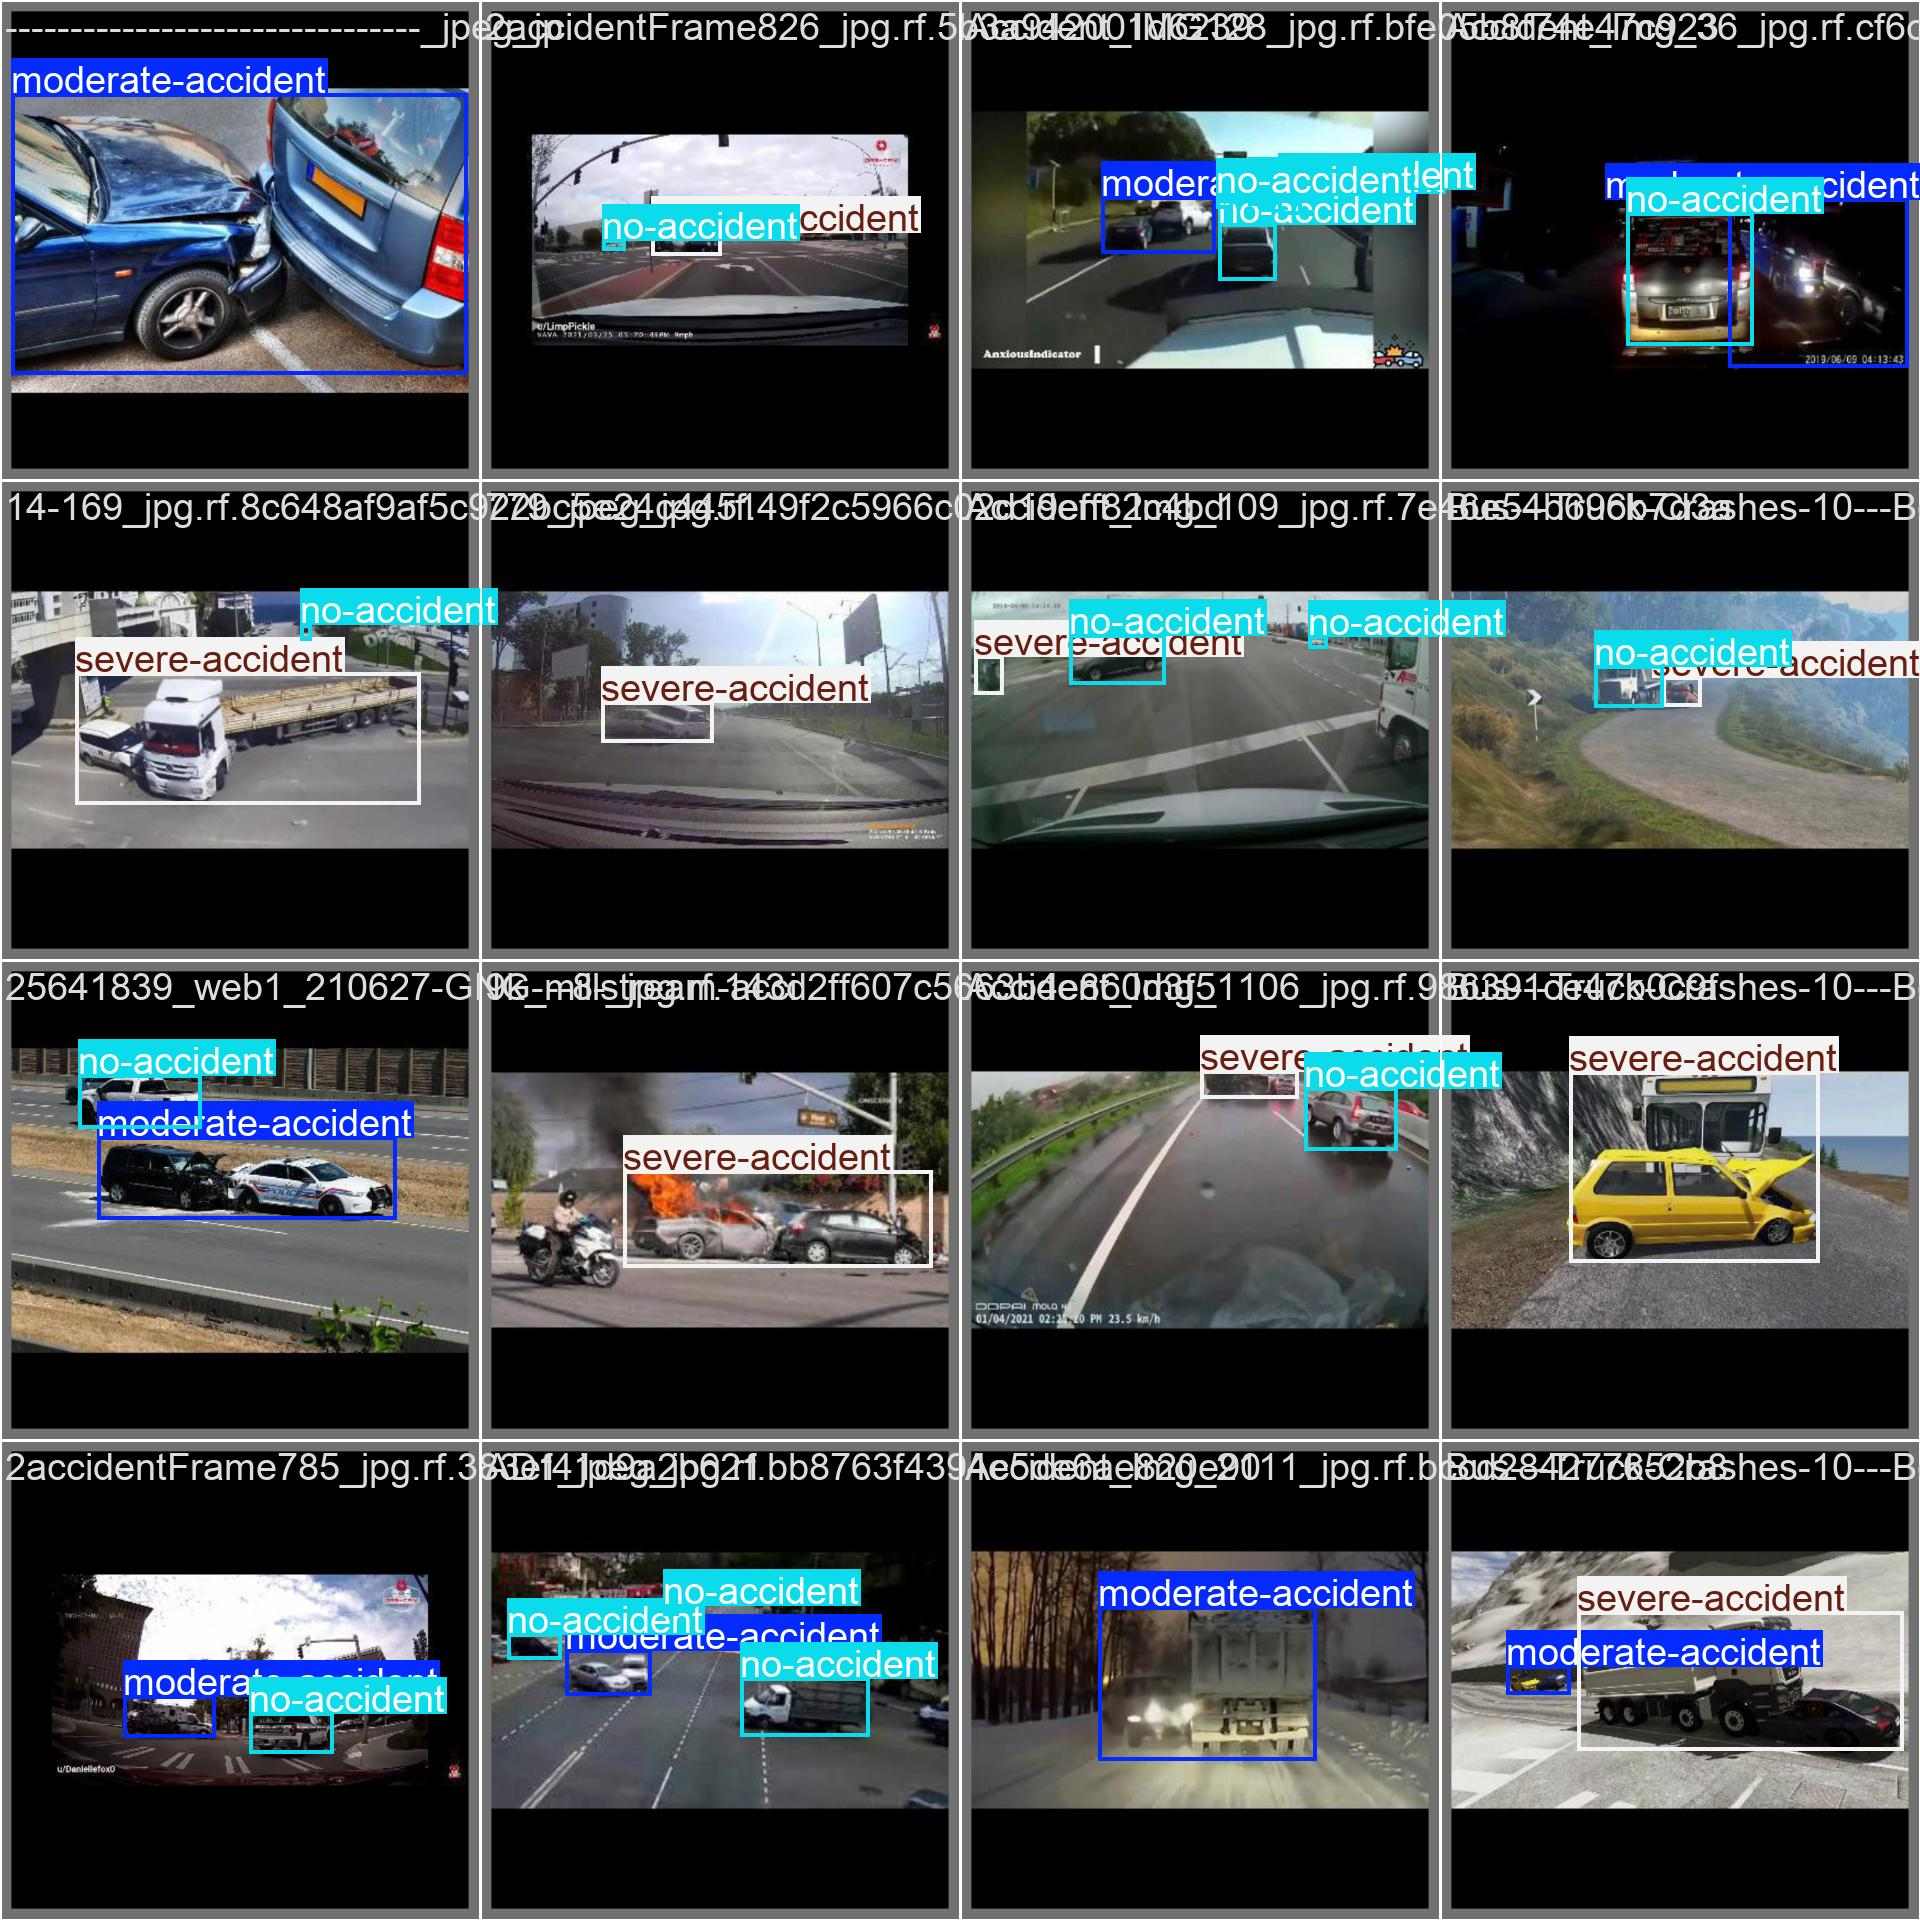
\includegraphics[width=\linewidth]{results/detection/accident_severity-2/val_batch0_labels.jpg}\end{minipage}
\begin{minipage}{0.32\textwidth}\centering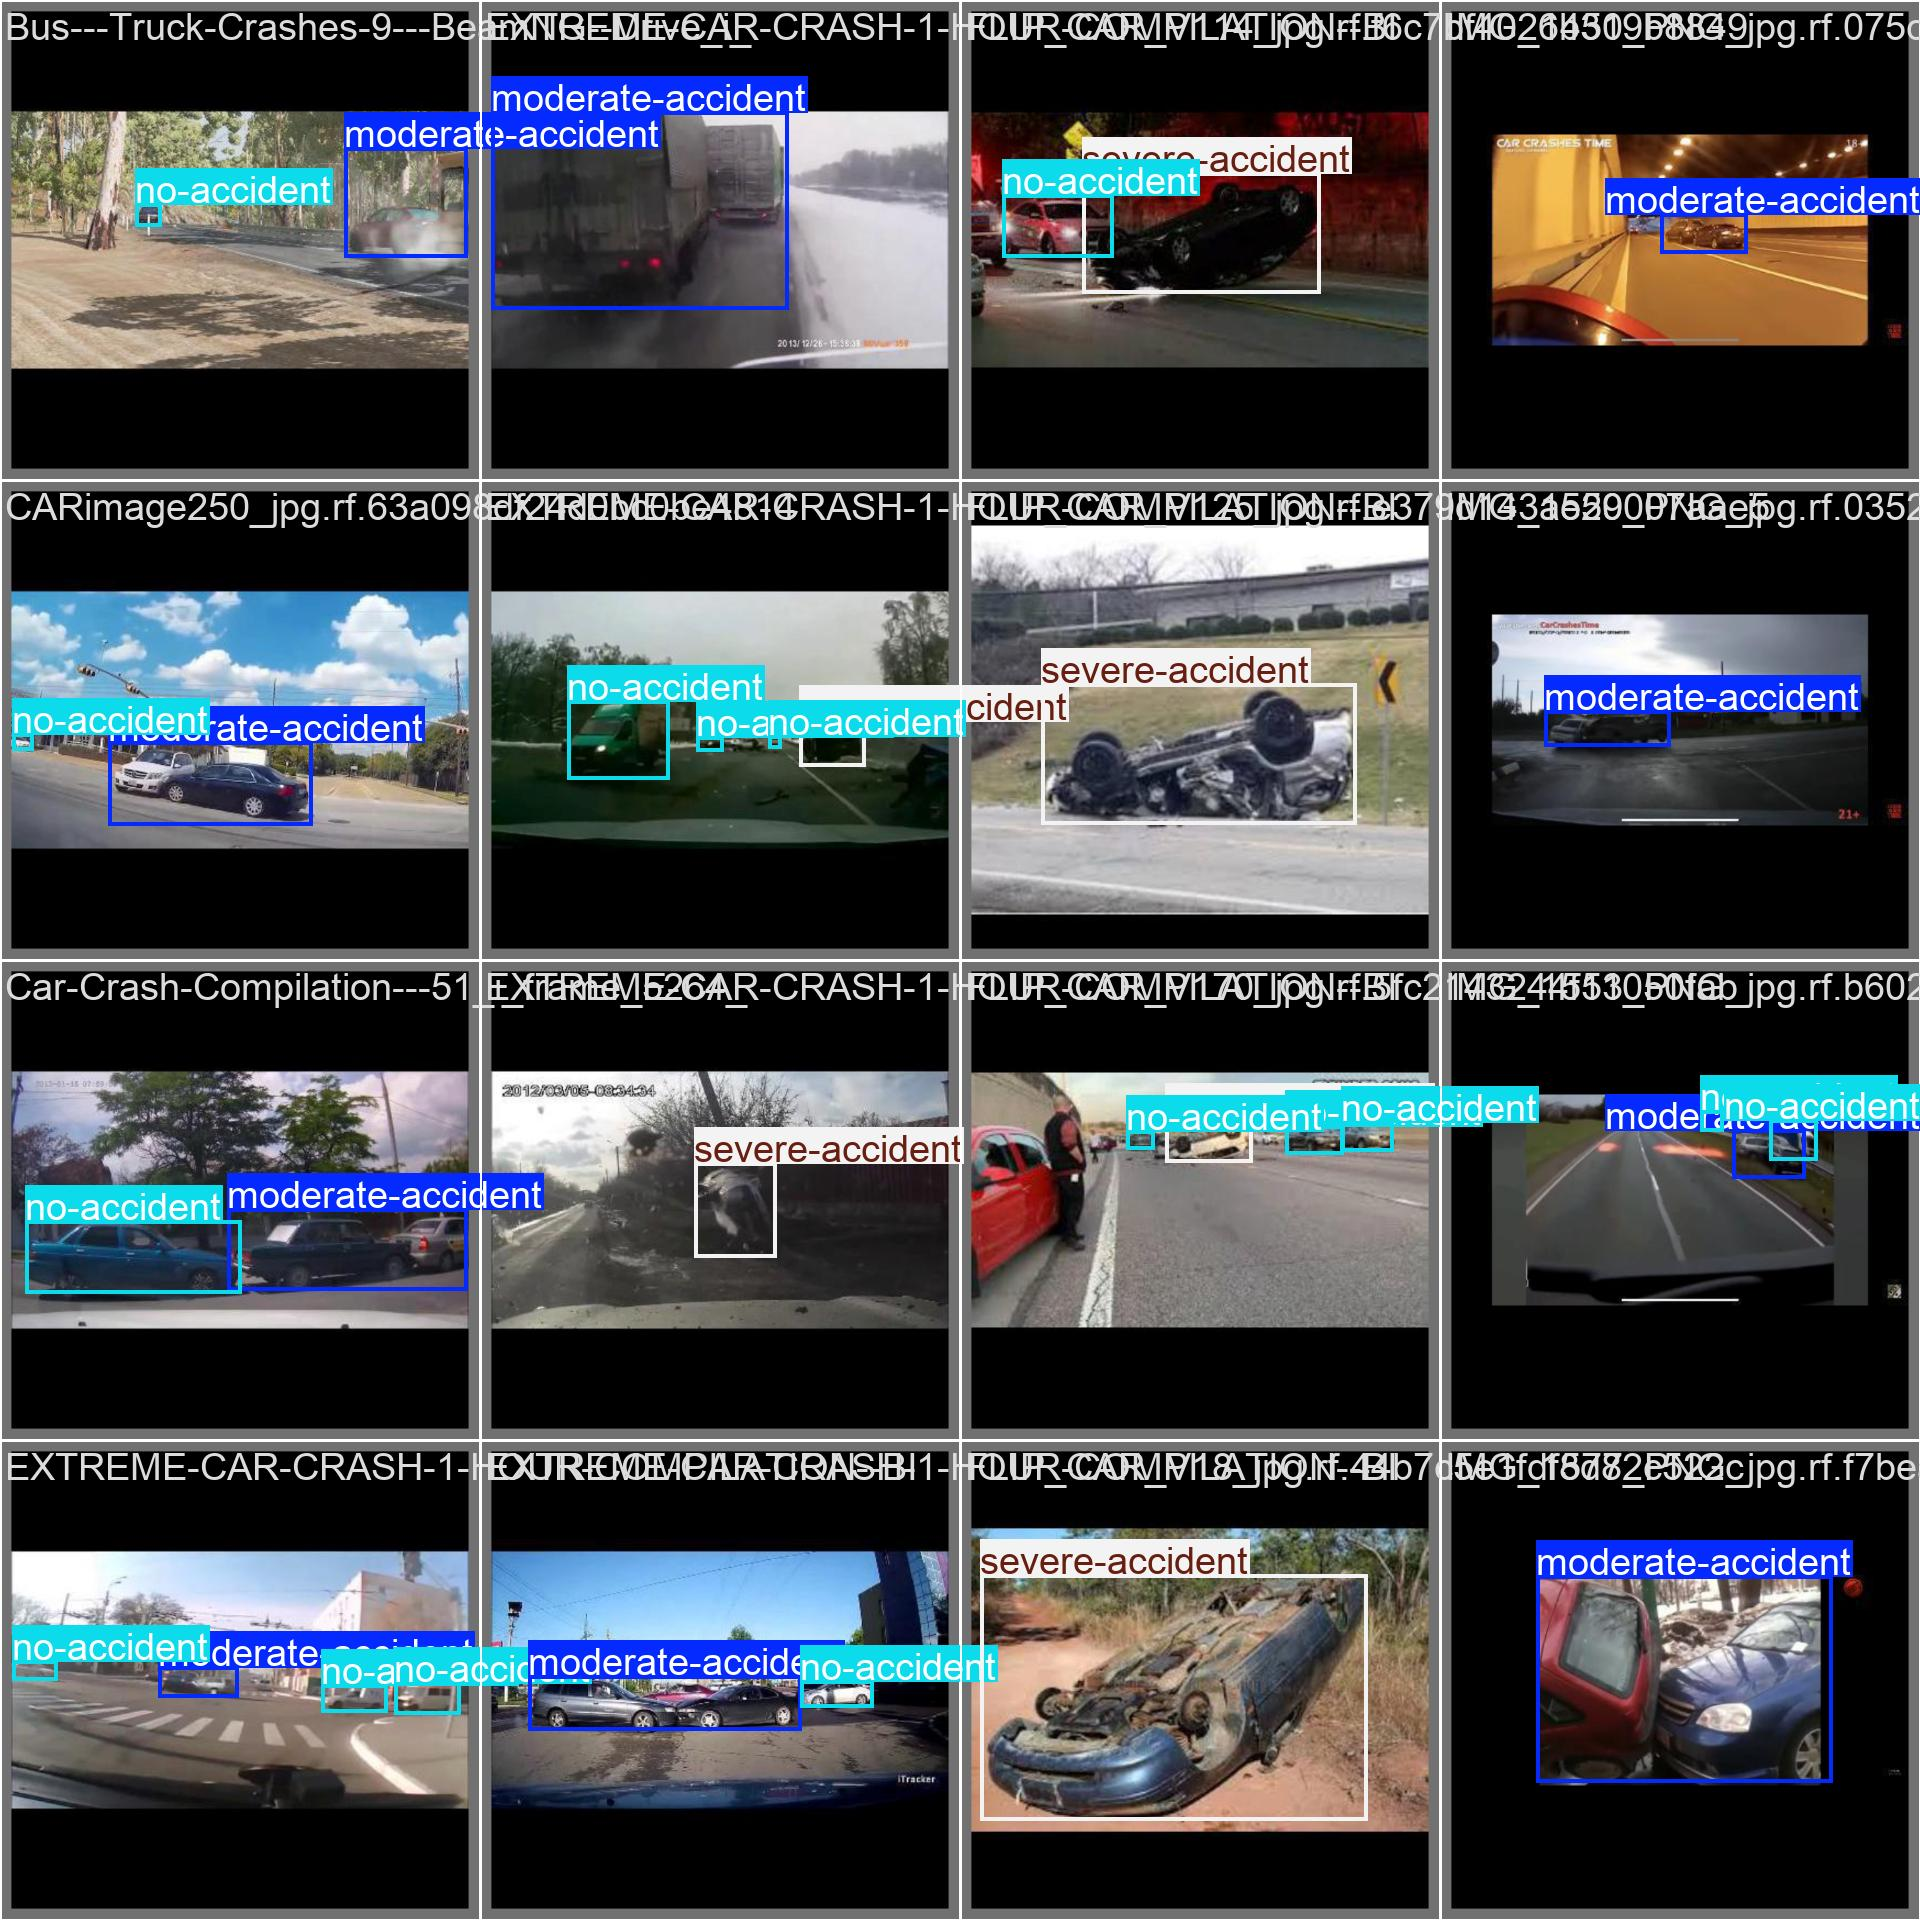
\includegraphics[width=\linewidth]{results/detection/accident_severity-2/val_batch1_labels.jpg}\end{minipage}
\begin{minipage}{0.32\textwidth}\centering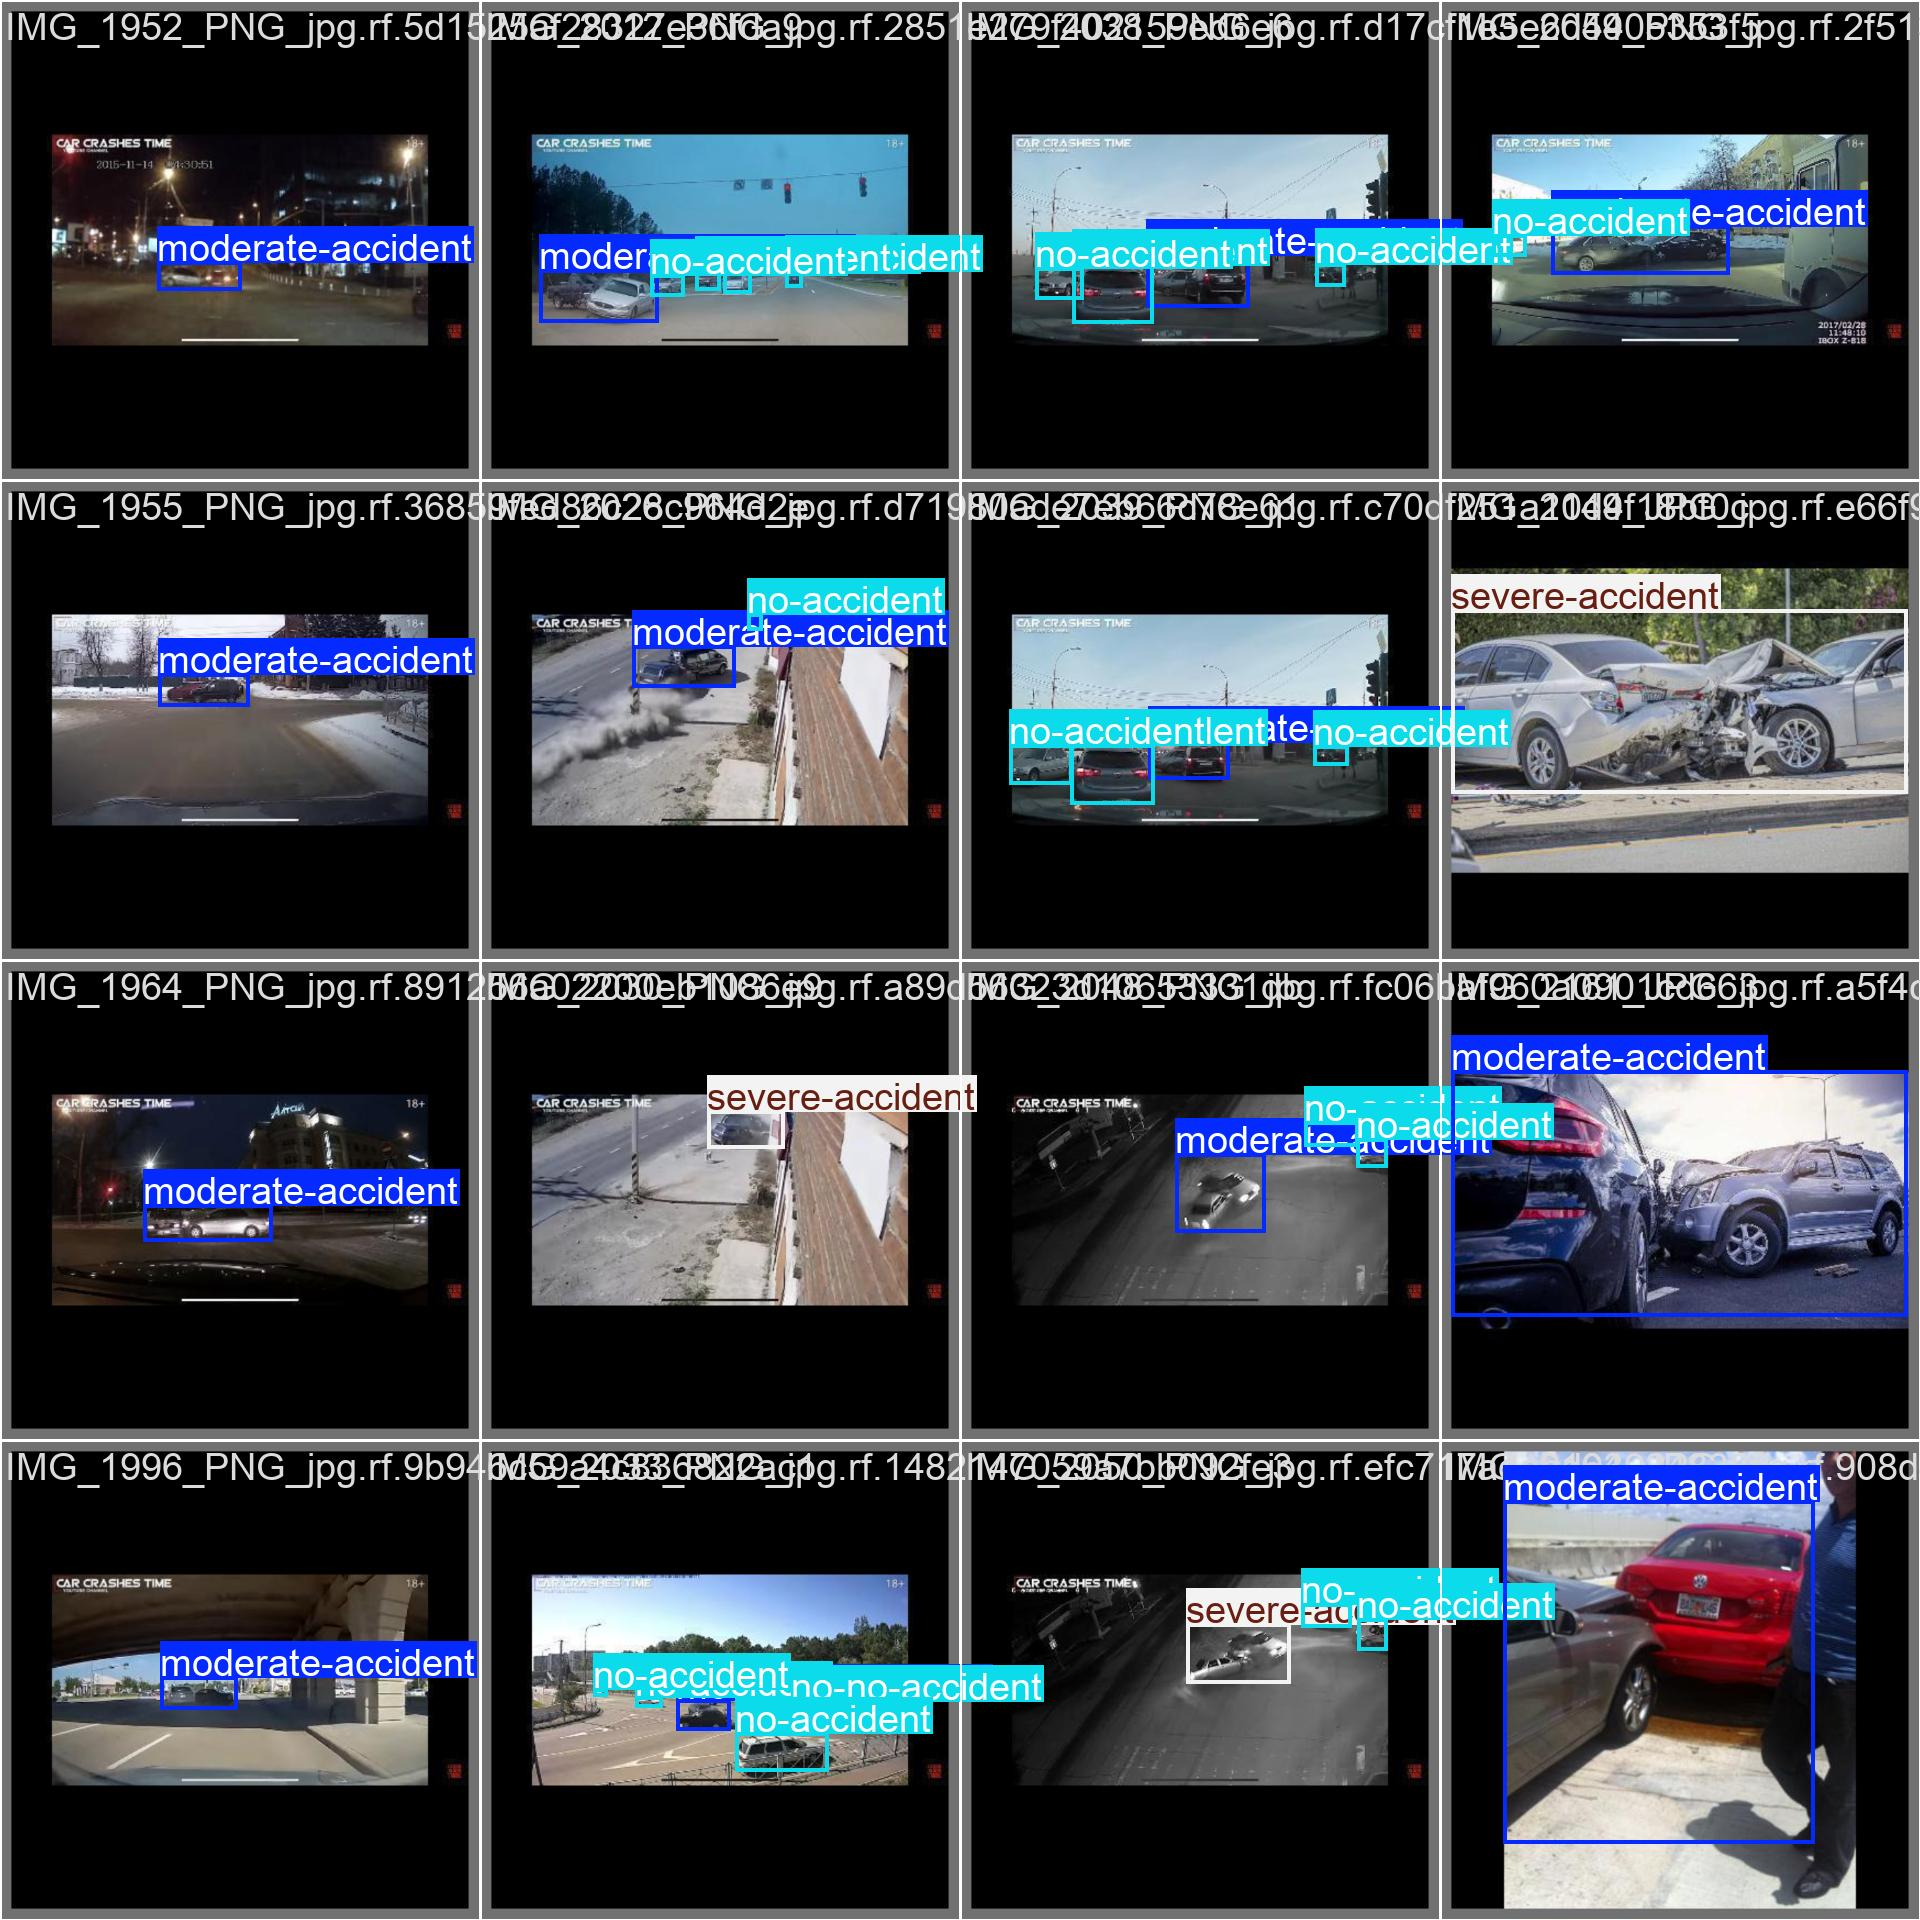
\includegraphics[width=\linewidth]{results/detection/accident_severity-2/val_batch2_labels.jpg}\end{minipage}
\par\vspace{4pt}
\begin{minipage}{0.32\textwidth}\centering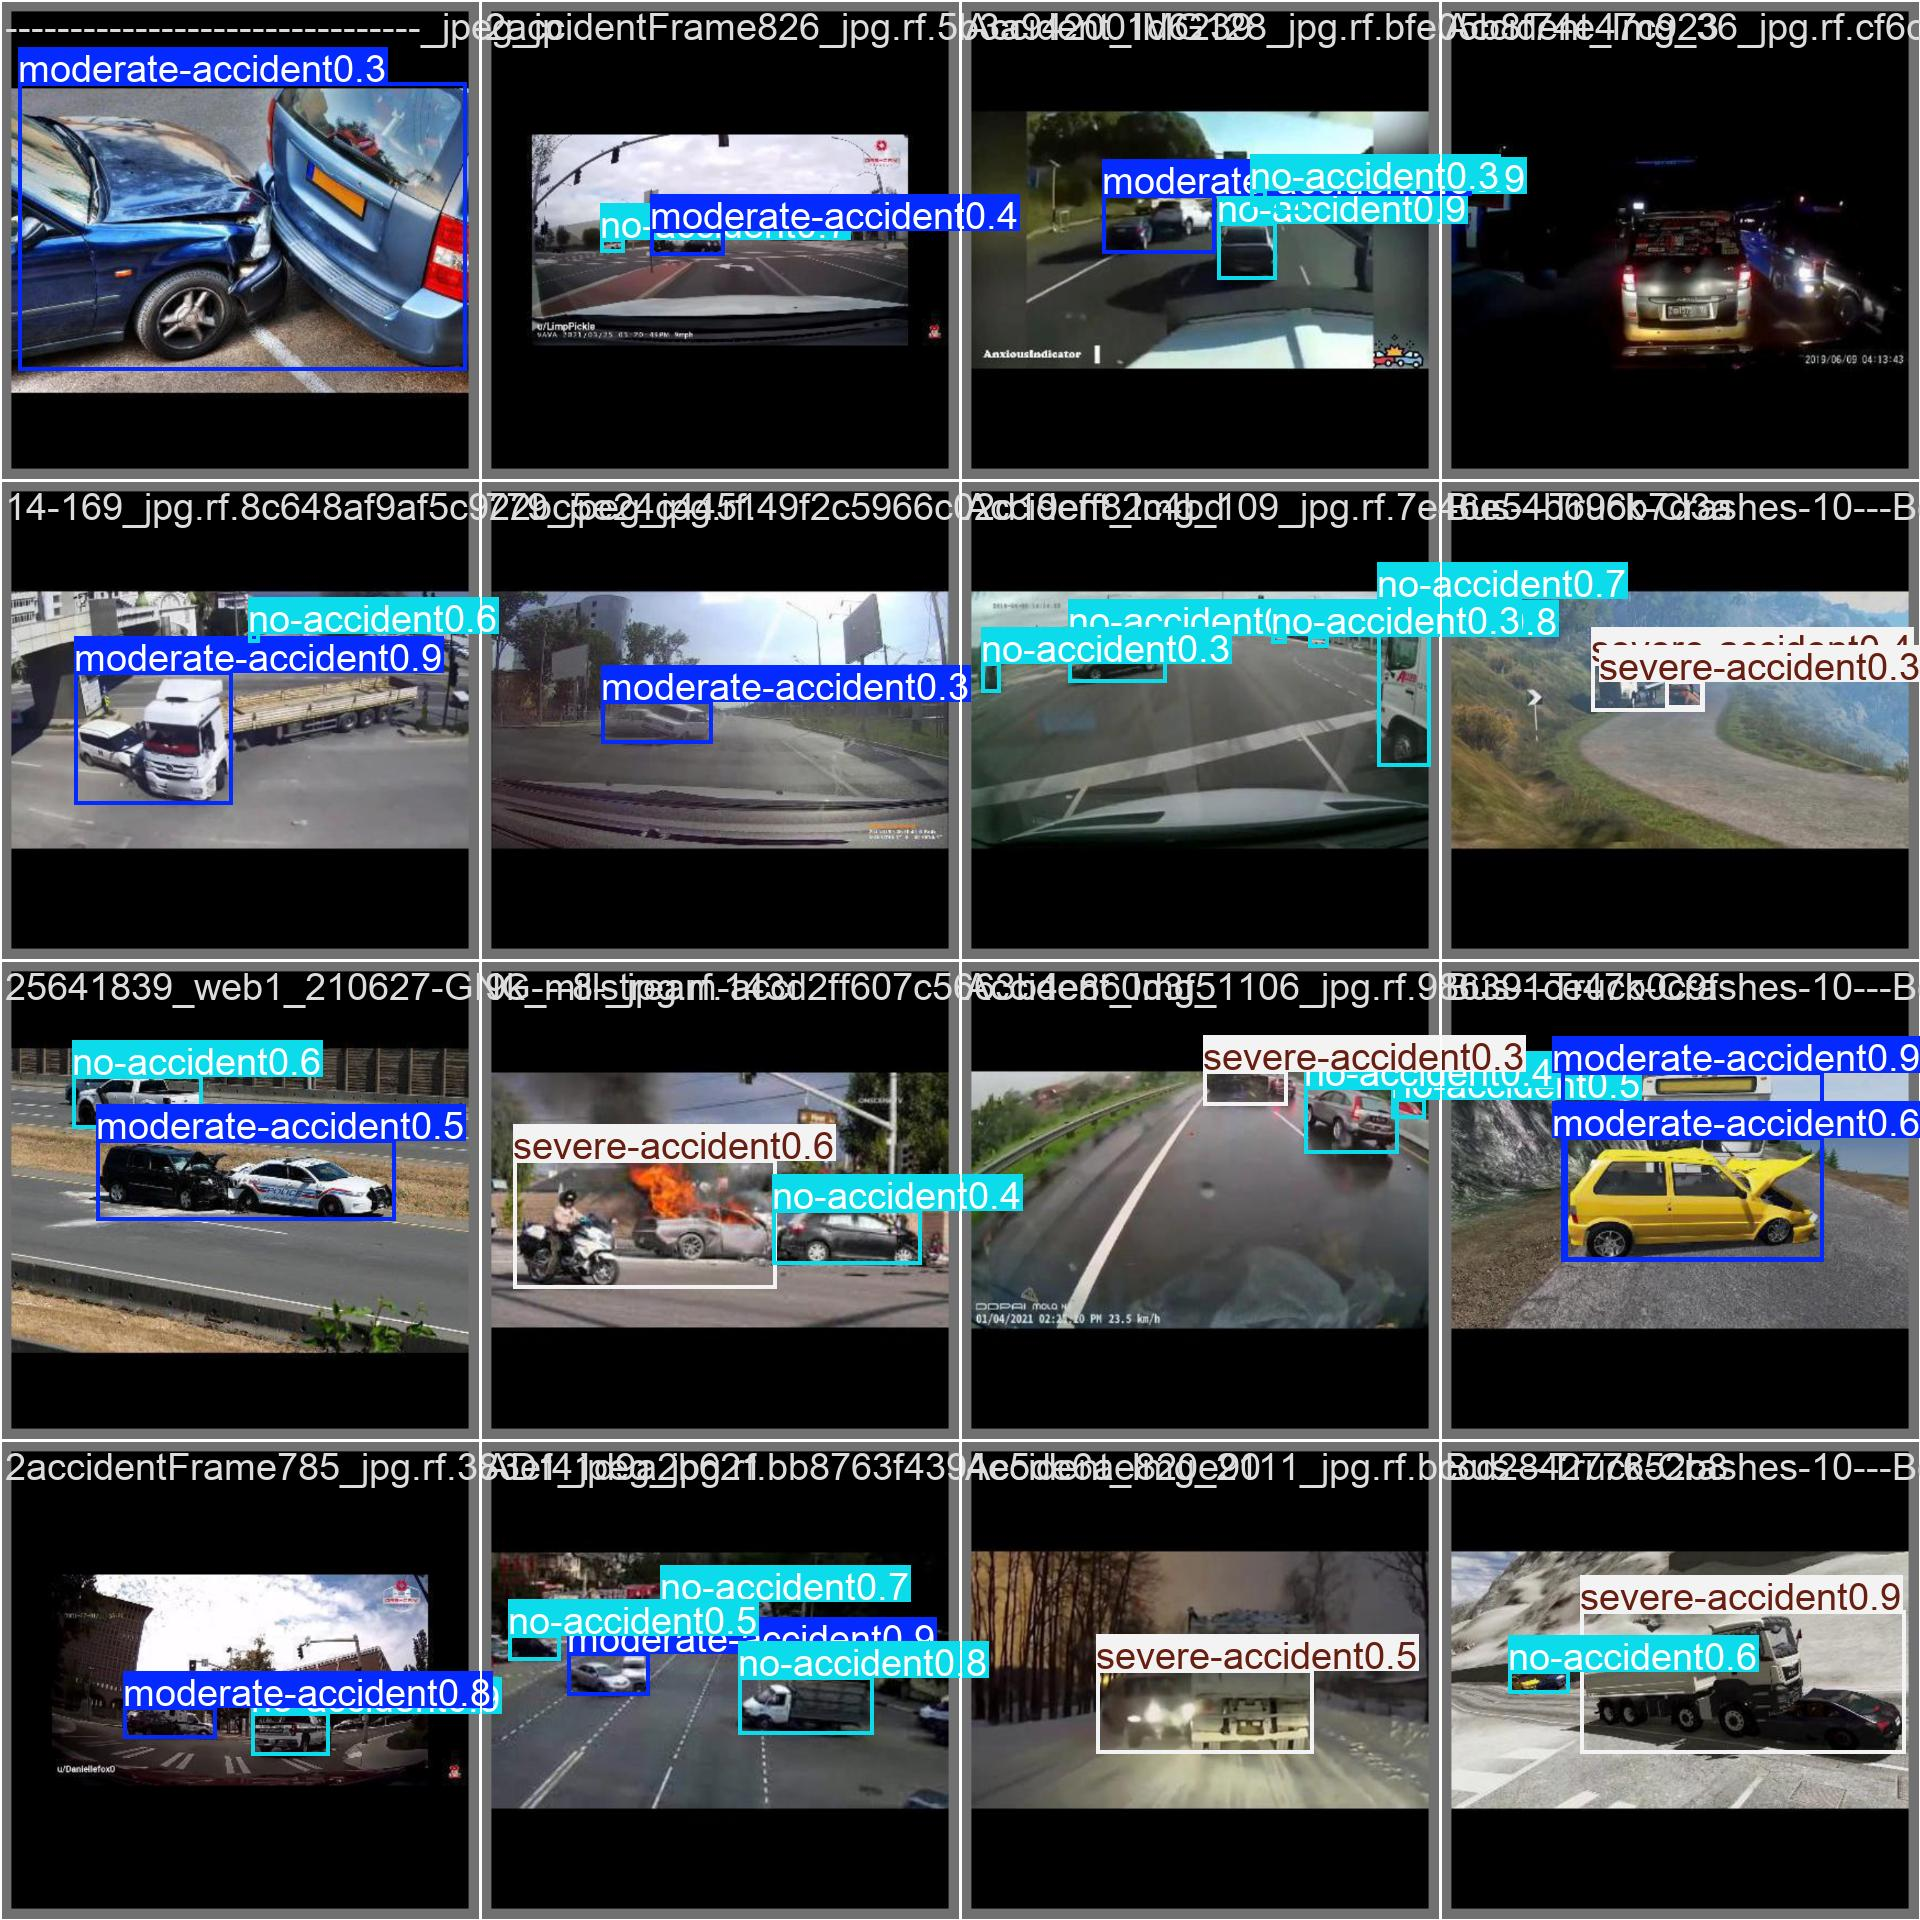
\includegraphics[width=\linewidth]{results/detection/accident_severity-2/val_batch0_pred.jpg}\end{minipage}
\begin{minipage}{0.32\textwidth}\centering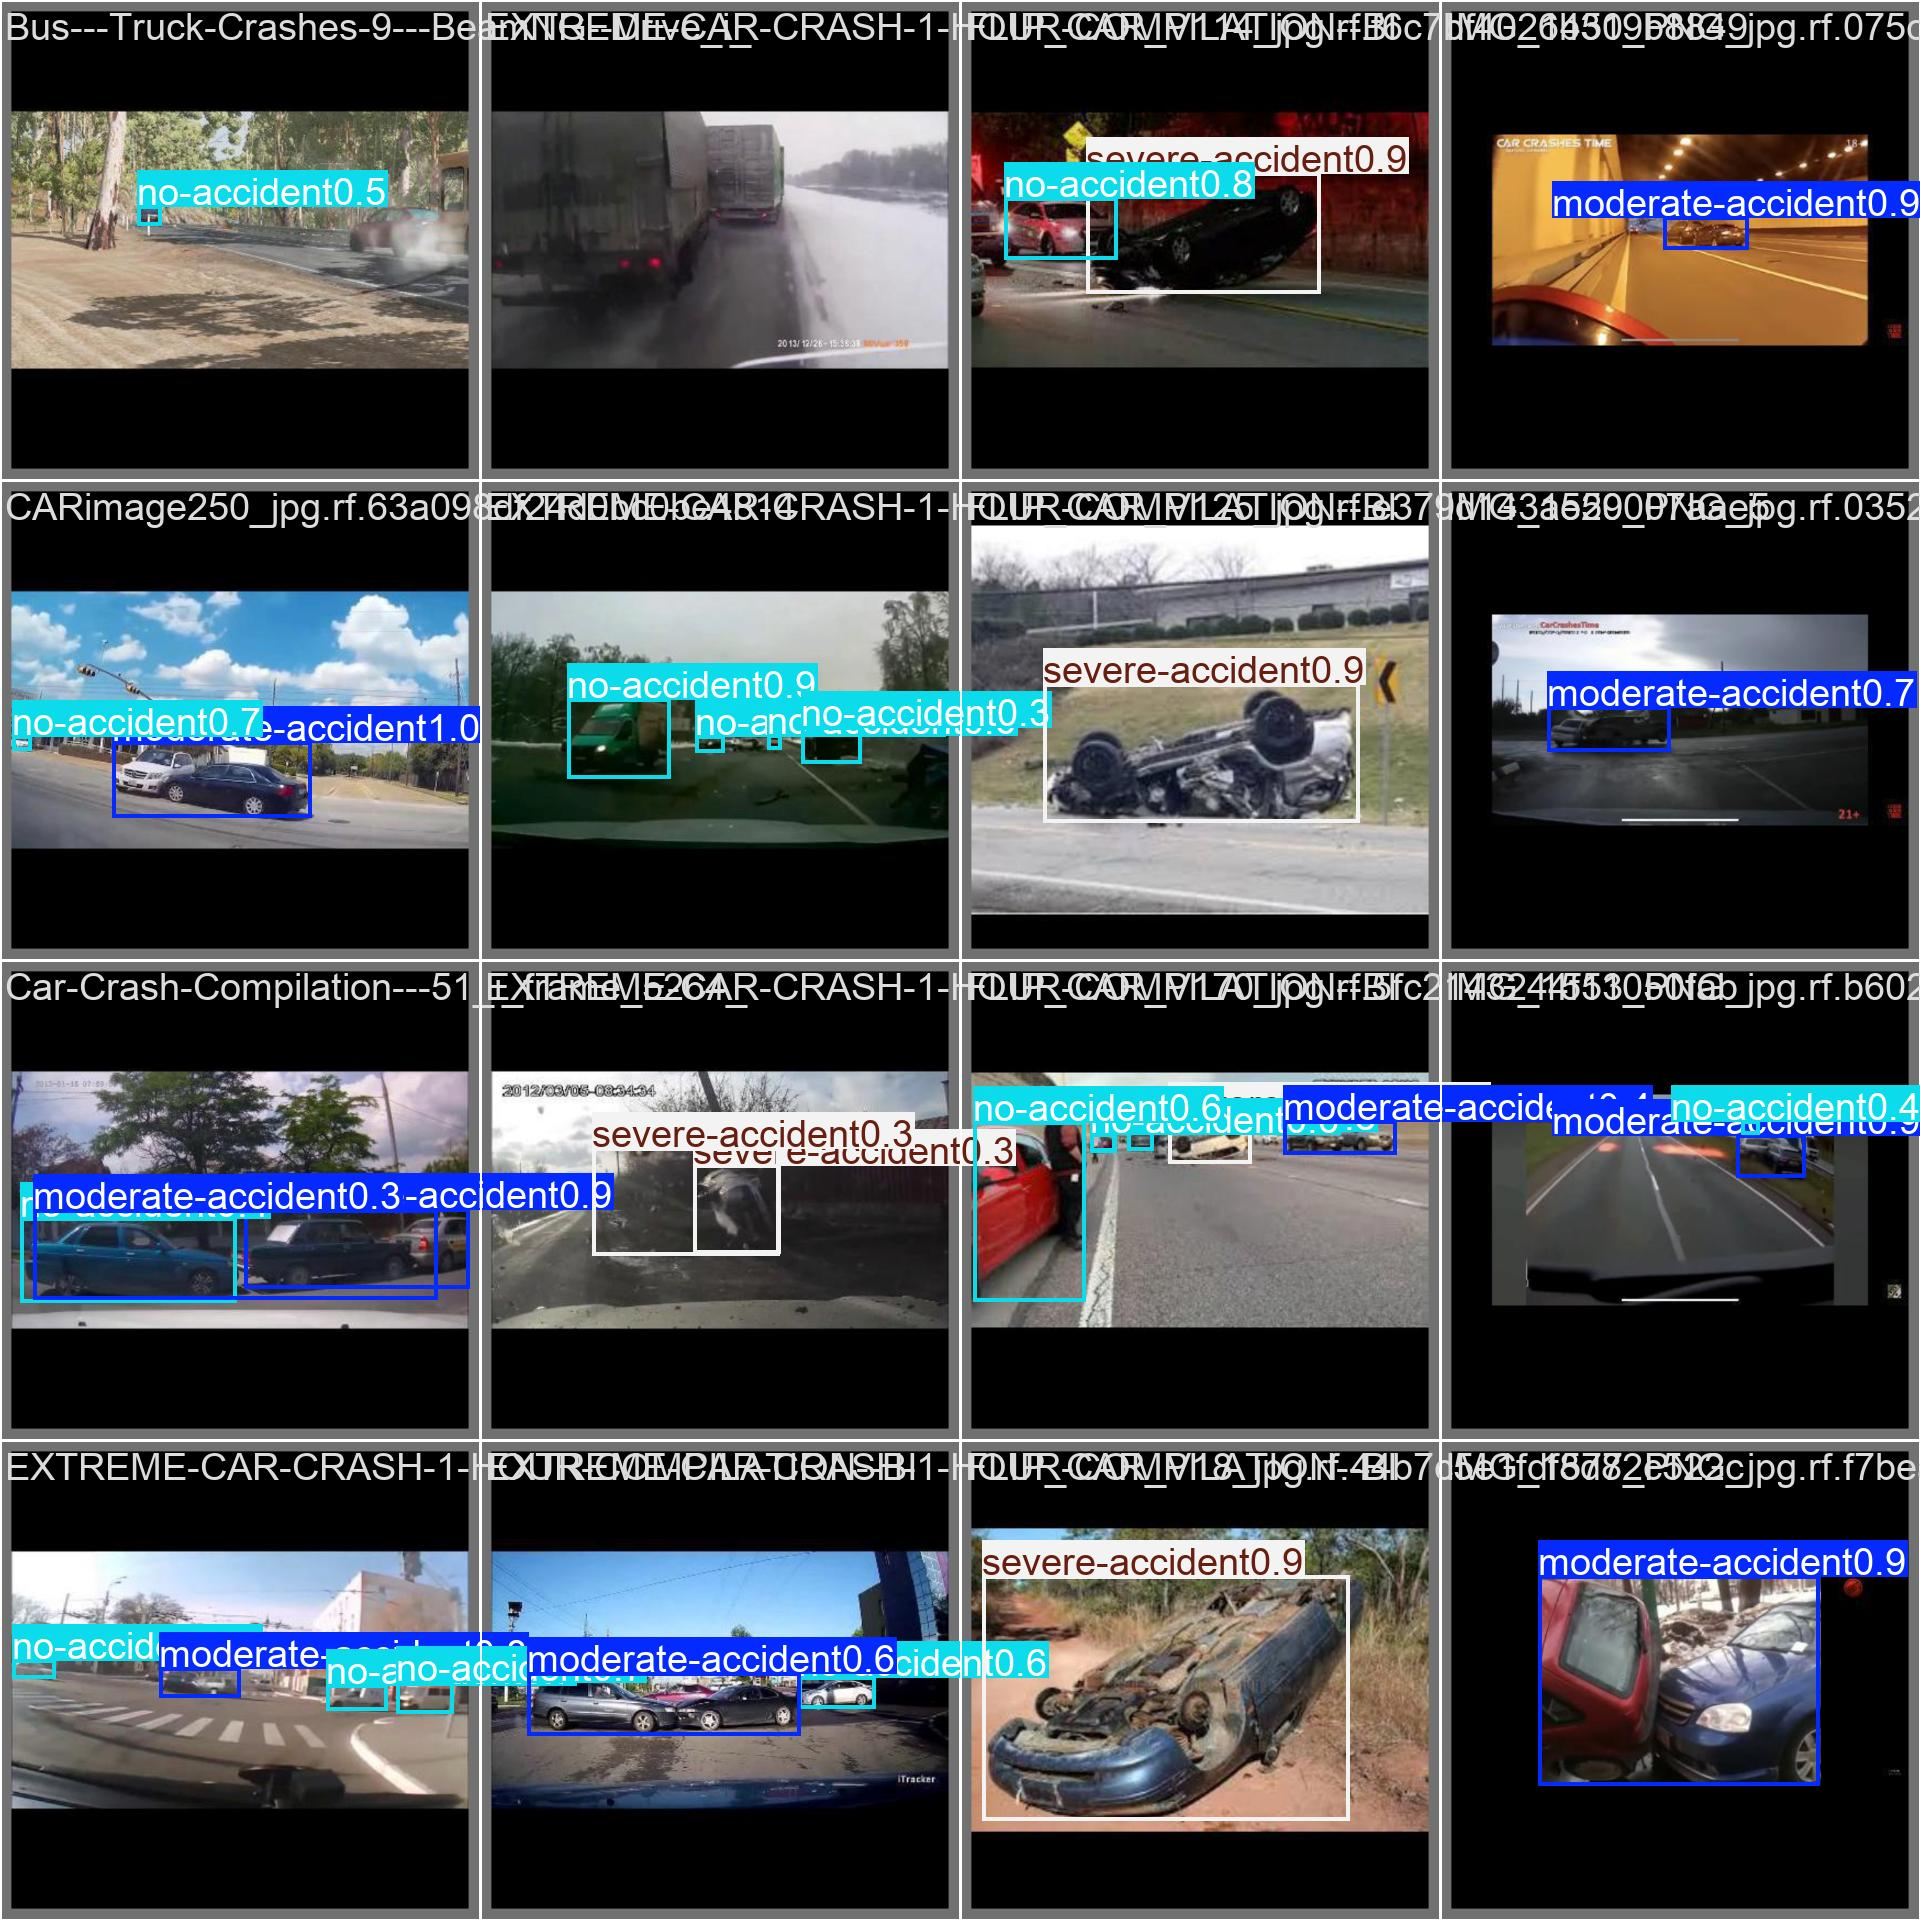
\includegraphics[width=\linewidth]{results/detection/accident_severity-2/val_batch1_pred.jpg}\end{minipage}
\begin{minipage}{0.32\textwidth}\centering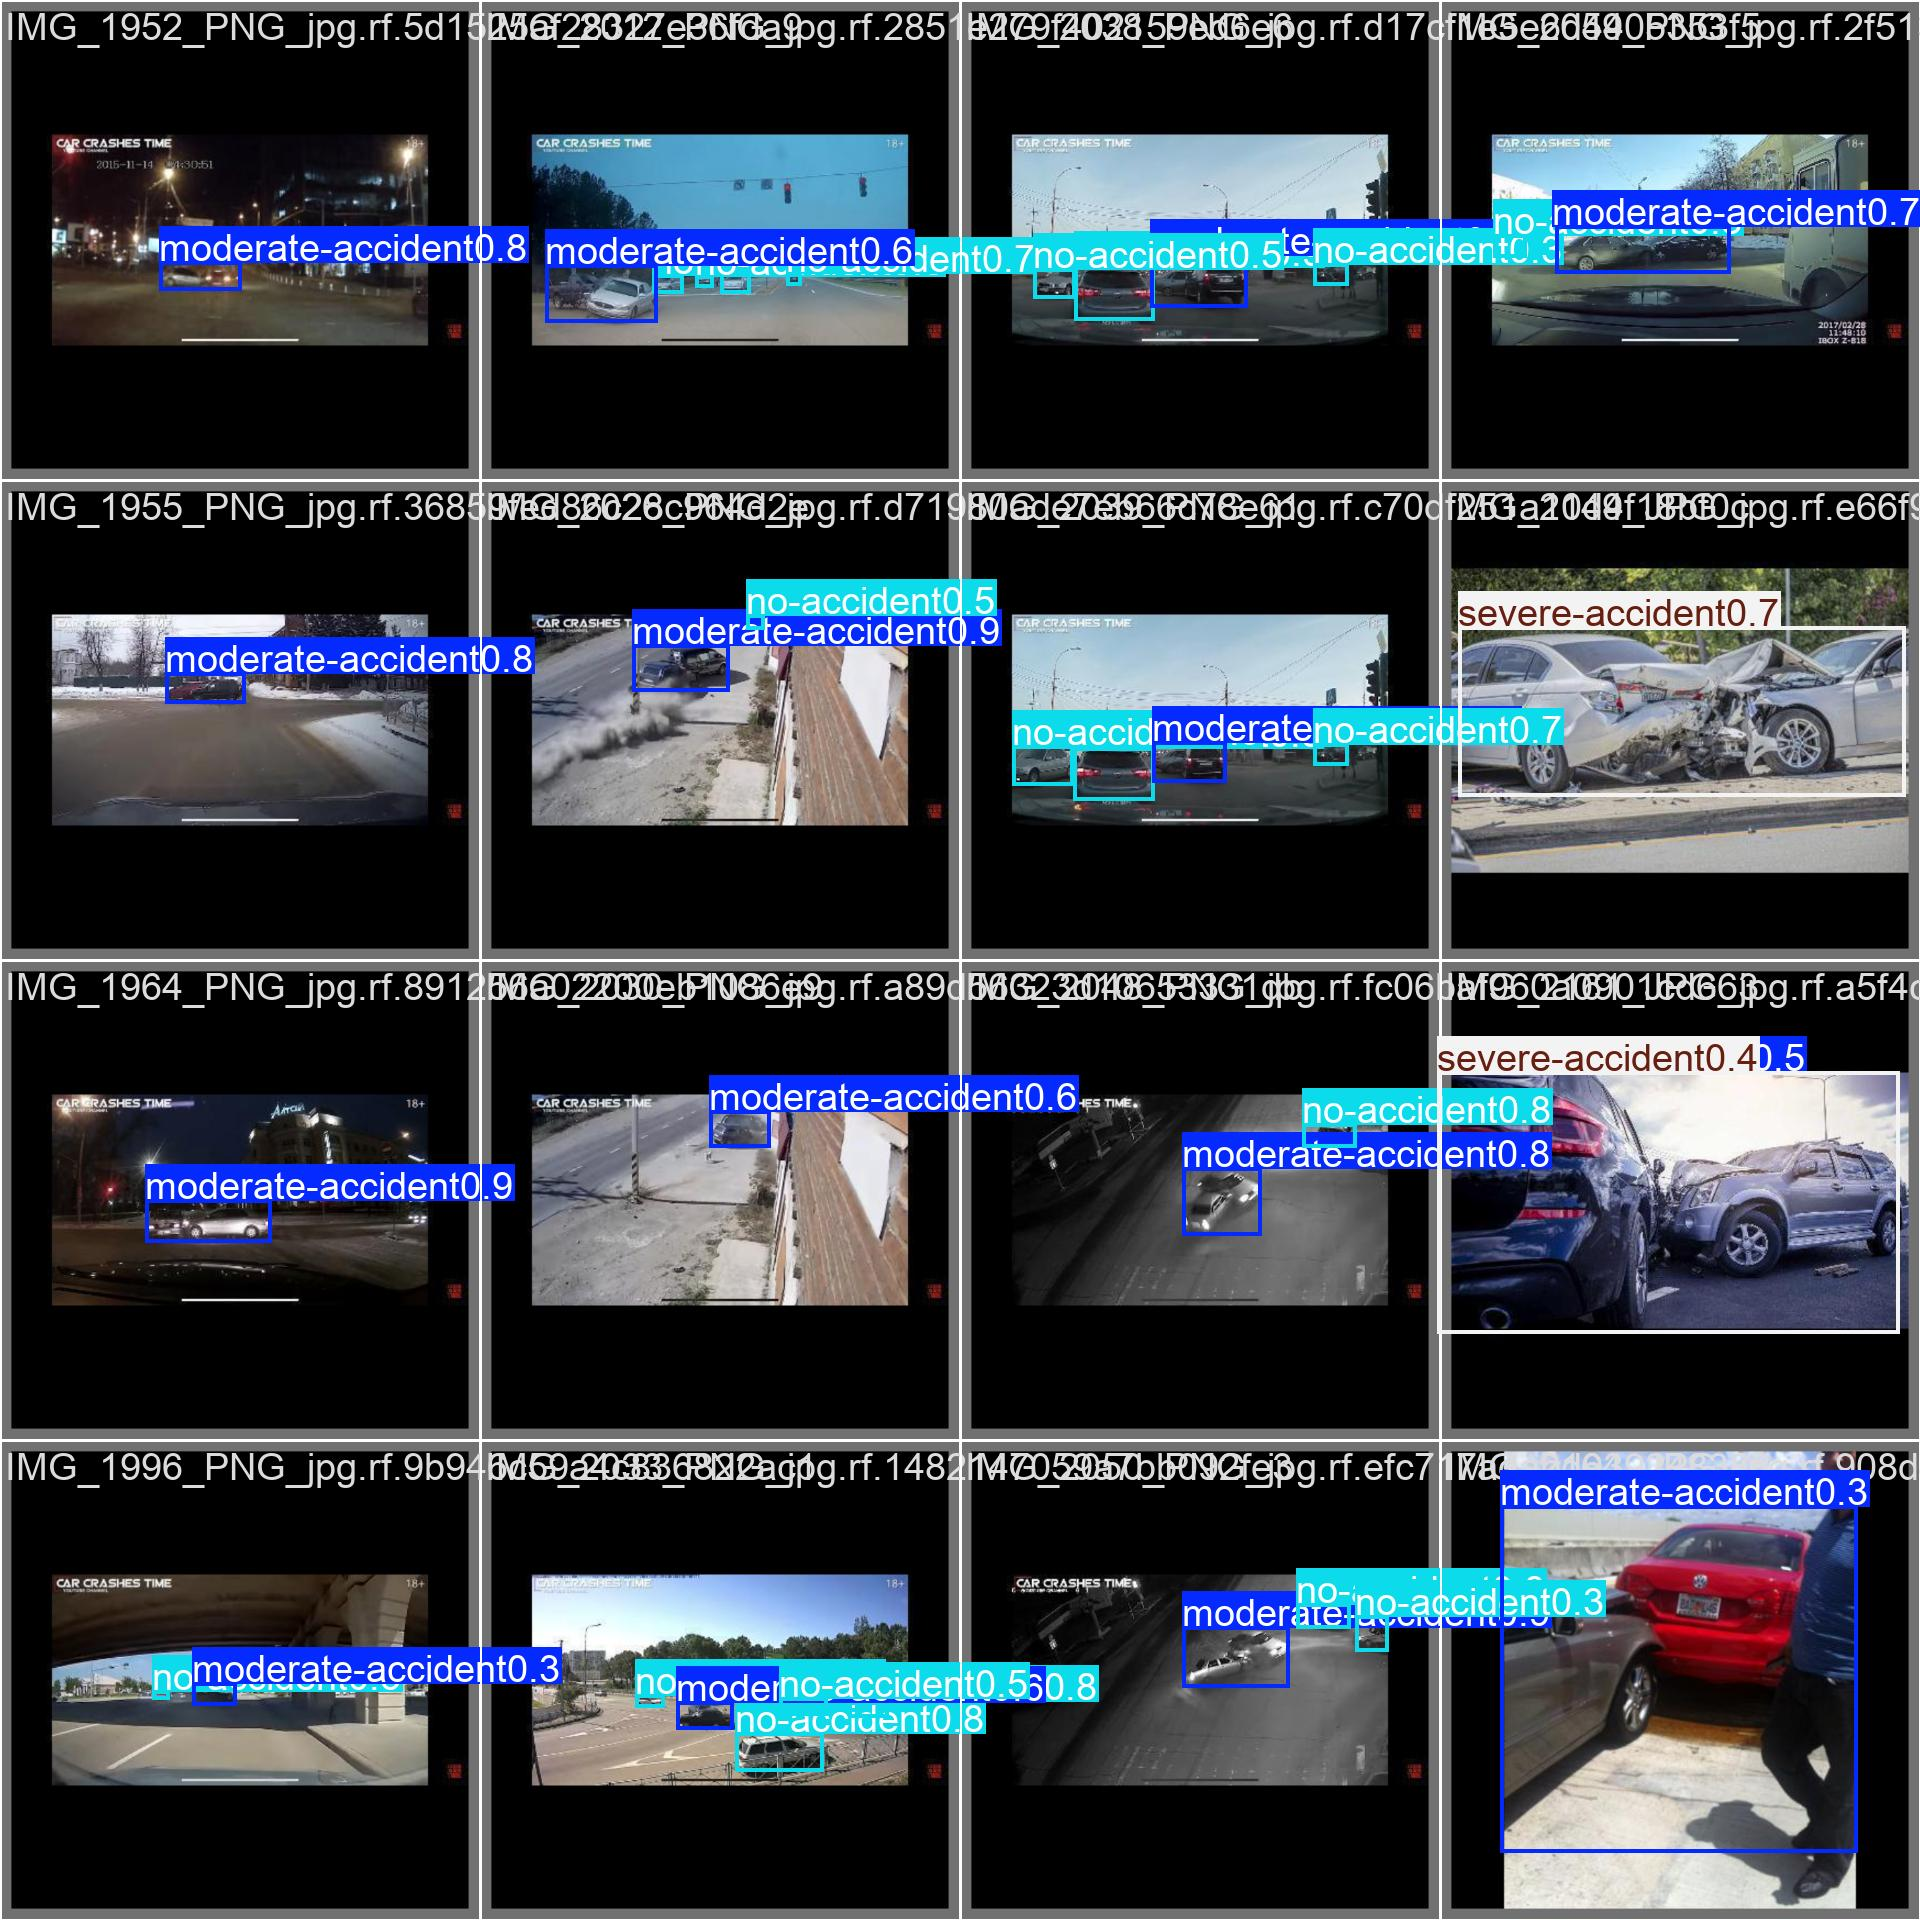
\includegraphics[width=\linewidth]{results/detection/accident_severity-2/val_batch2_pred.jpg}\end{minipage}
\caption{All saved validation batches for Accident Severity: ground-truth labels above and predictions below.}
\end{figure}
\section{Night Traffic Training and Validation Previews}
\begin{figure}[t]\centering
\begin{minipage}{0.32\textwidth}\centering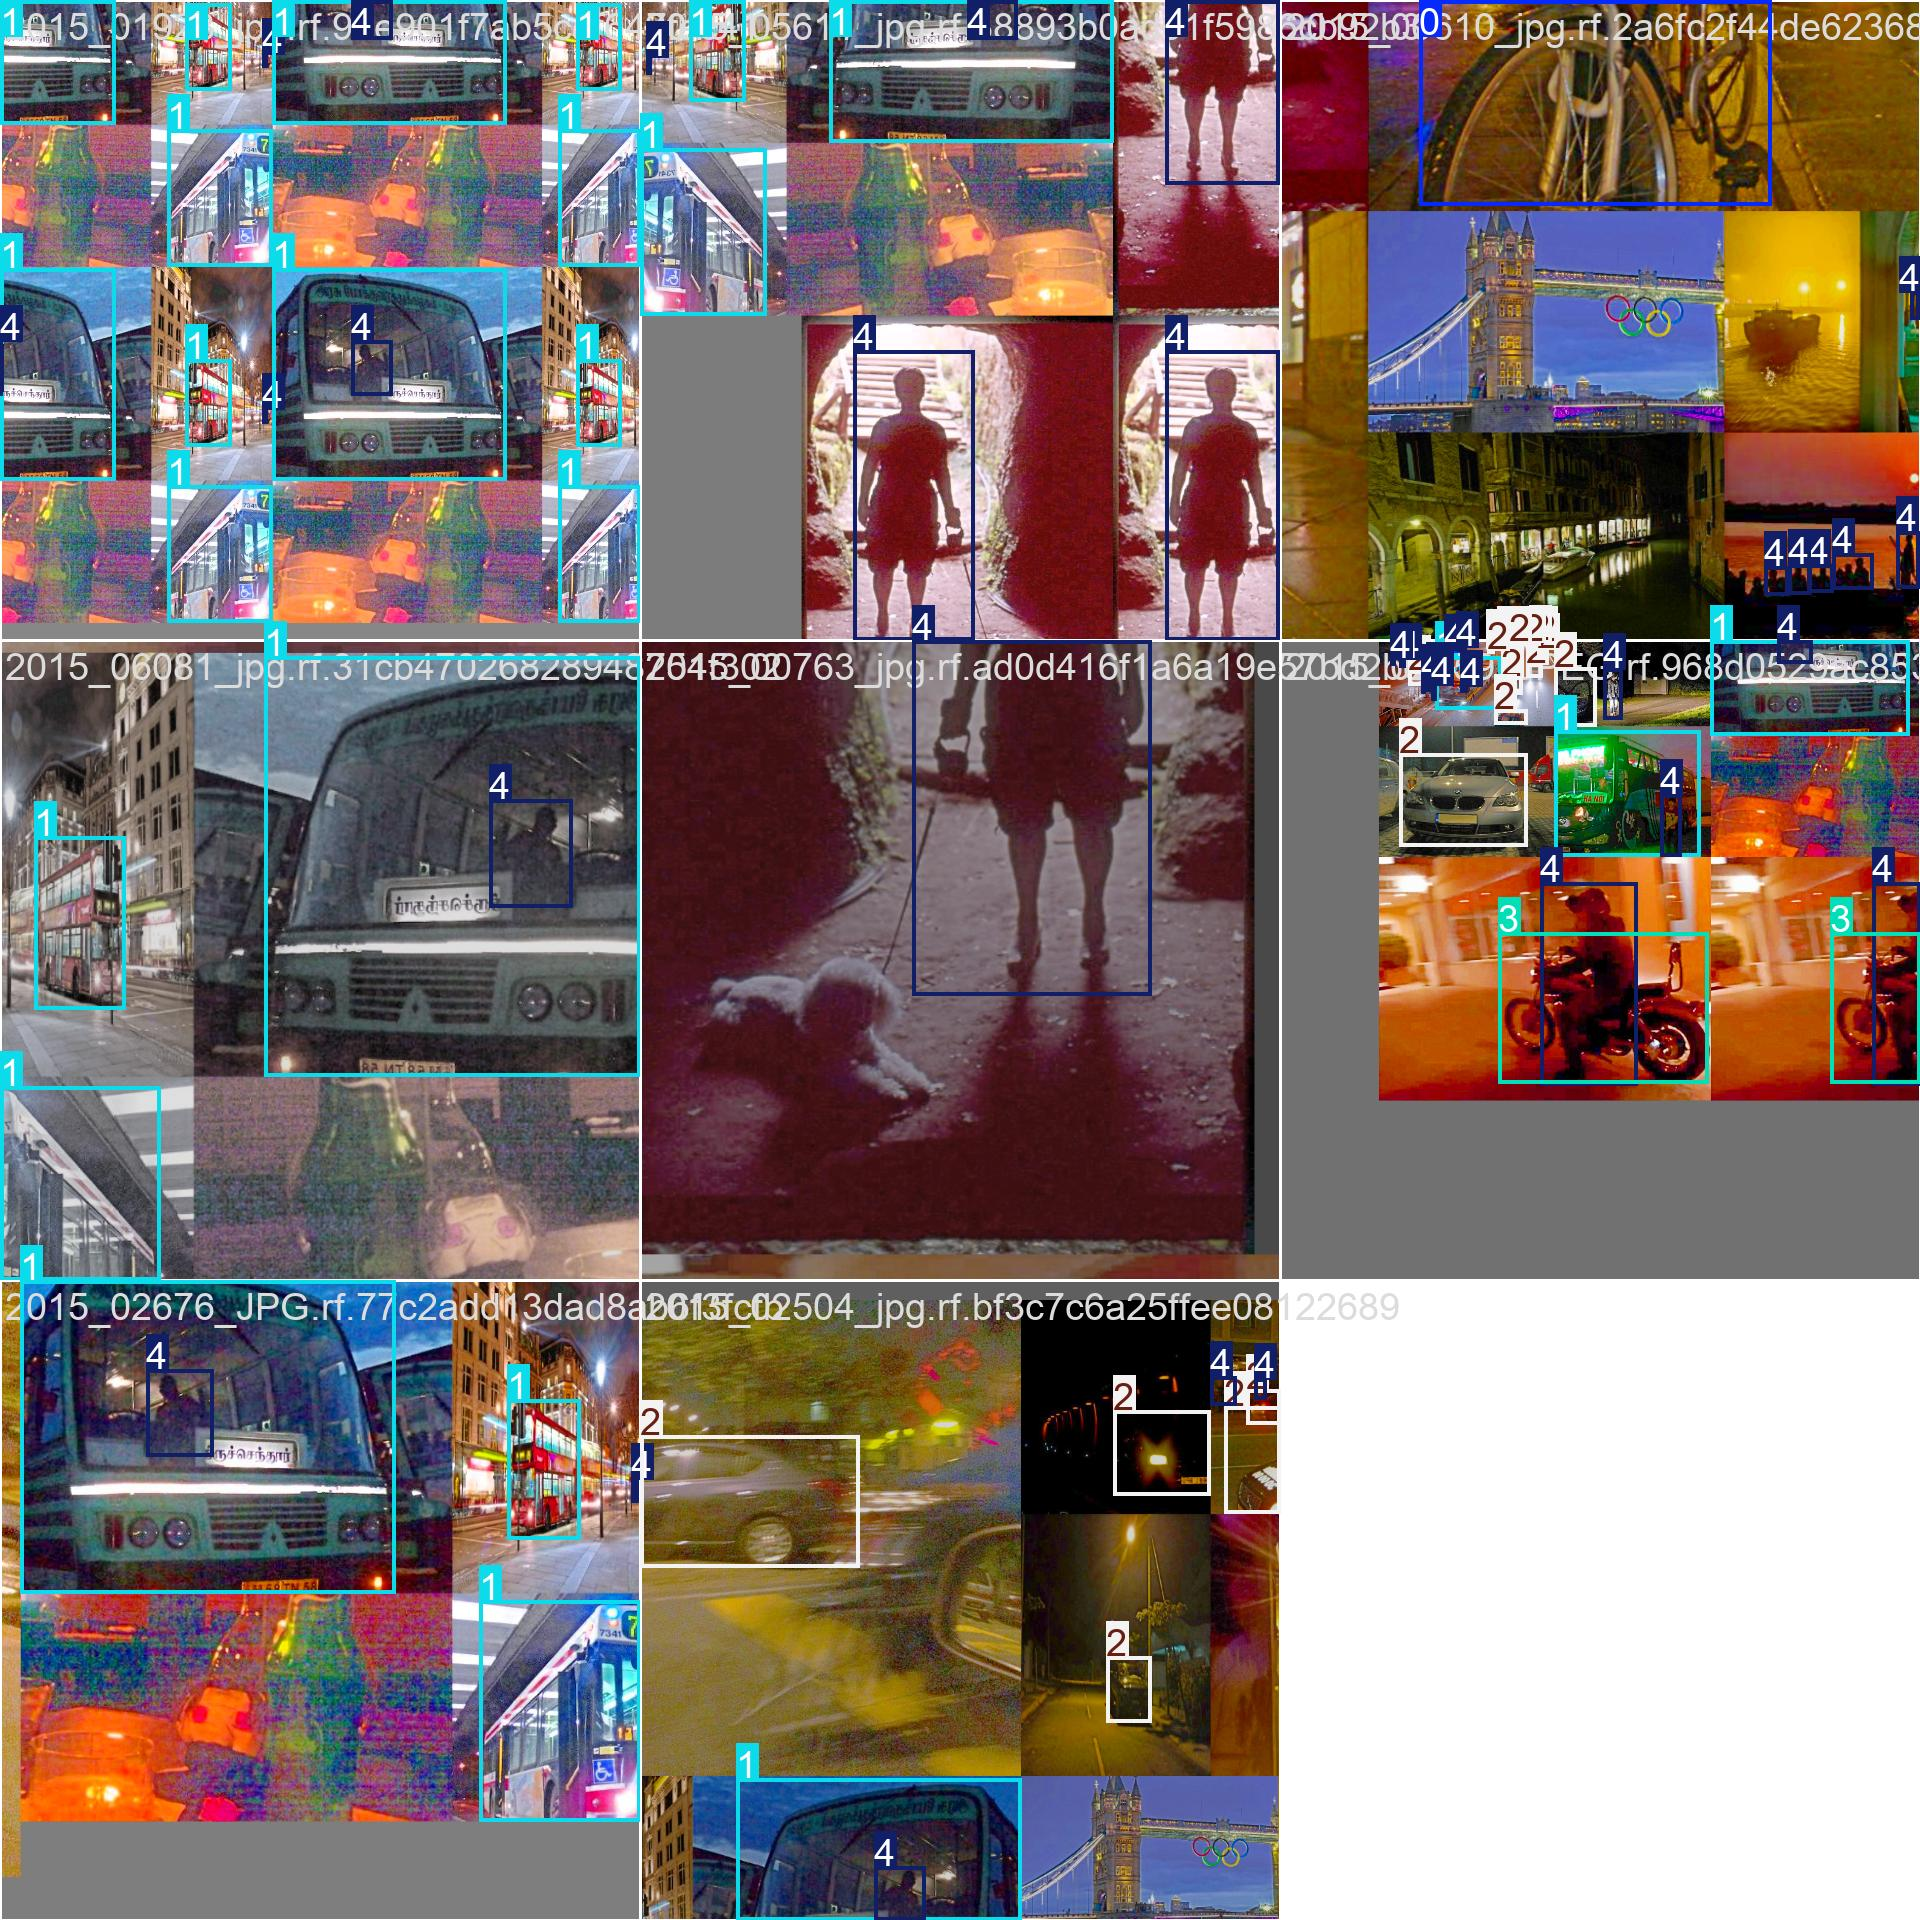
\includegraphics[width=\linewidth]{results/detection/night_traffic-2/train_batch0.jpg}\end{minipage}
\begin{minipage}{0.32\textwidth}\centering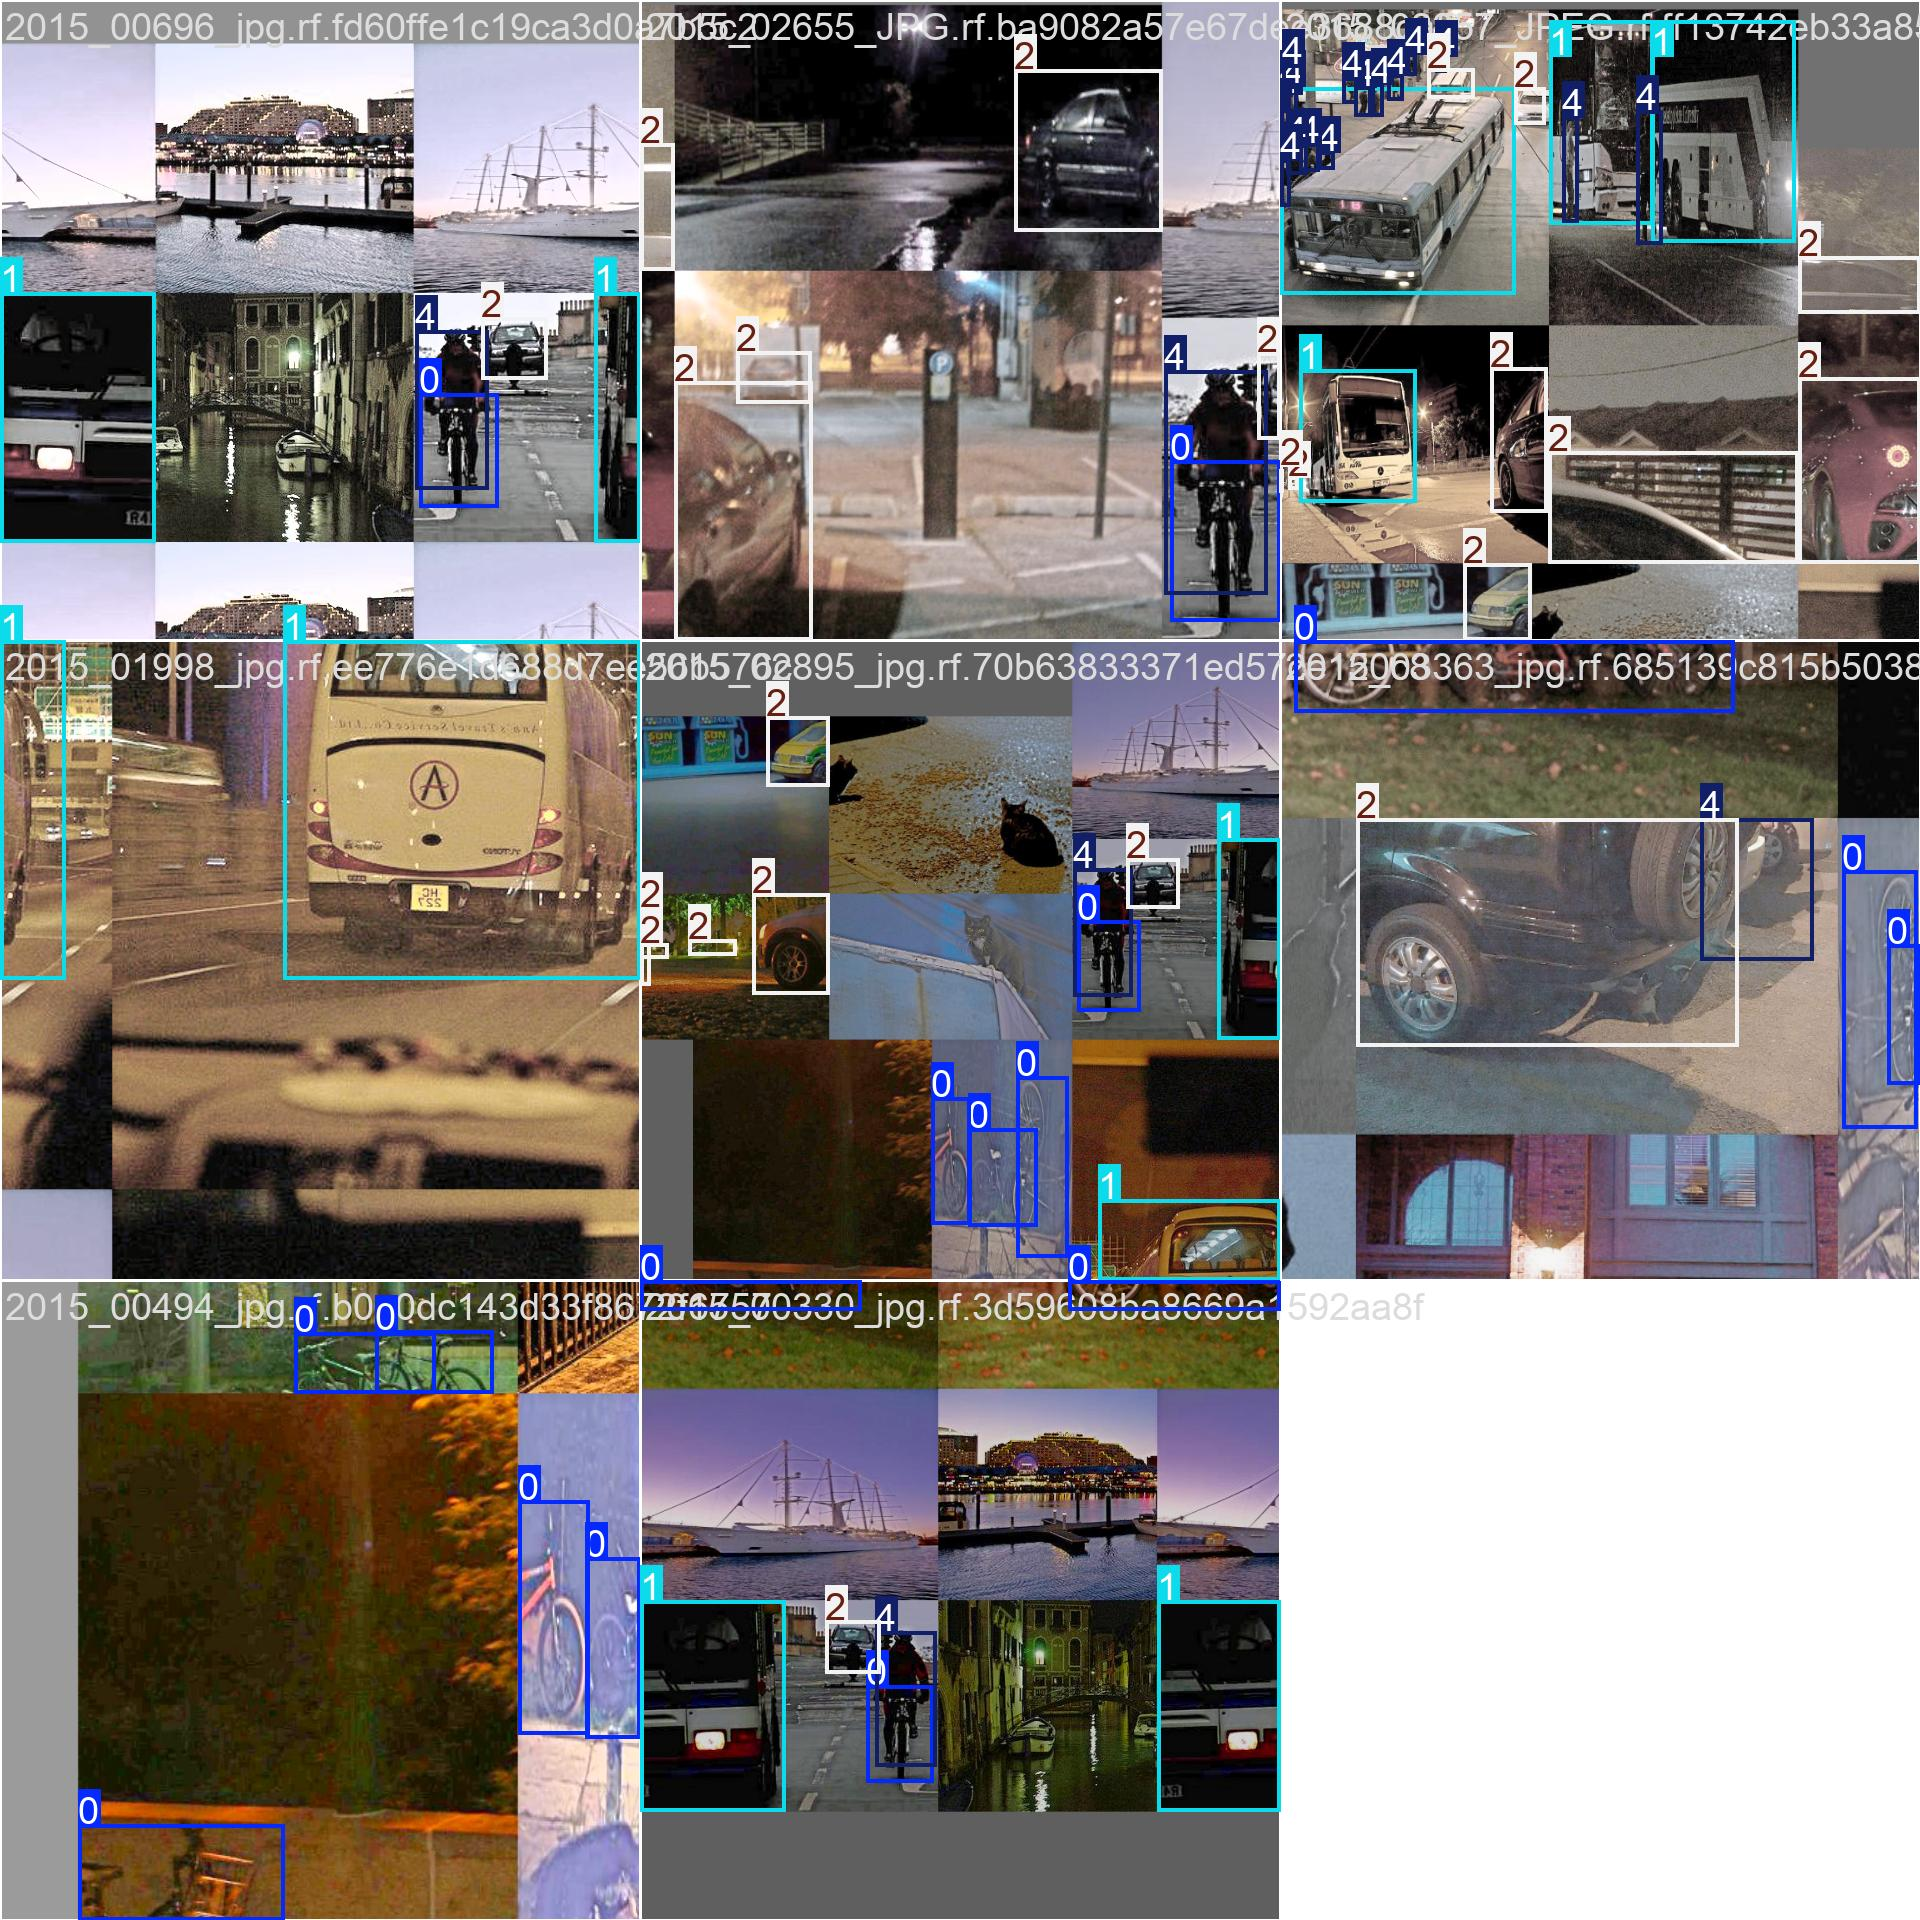
\includegraphics[width=\linewidth]{results/detection/night_traffic-2/train_batch1.jpg}\end{minipage}
\begin{minipage}{0.32\textwidth}\centering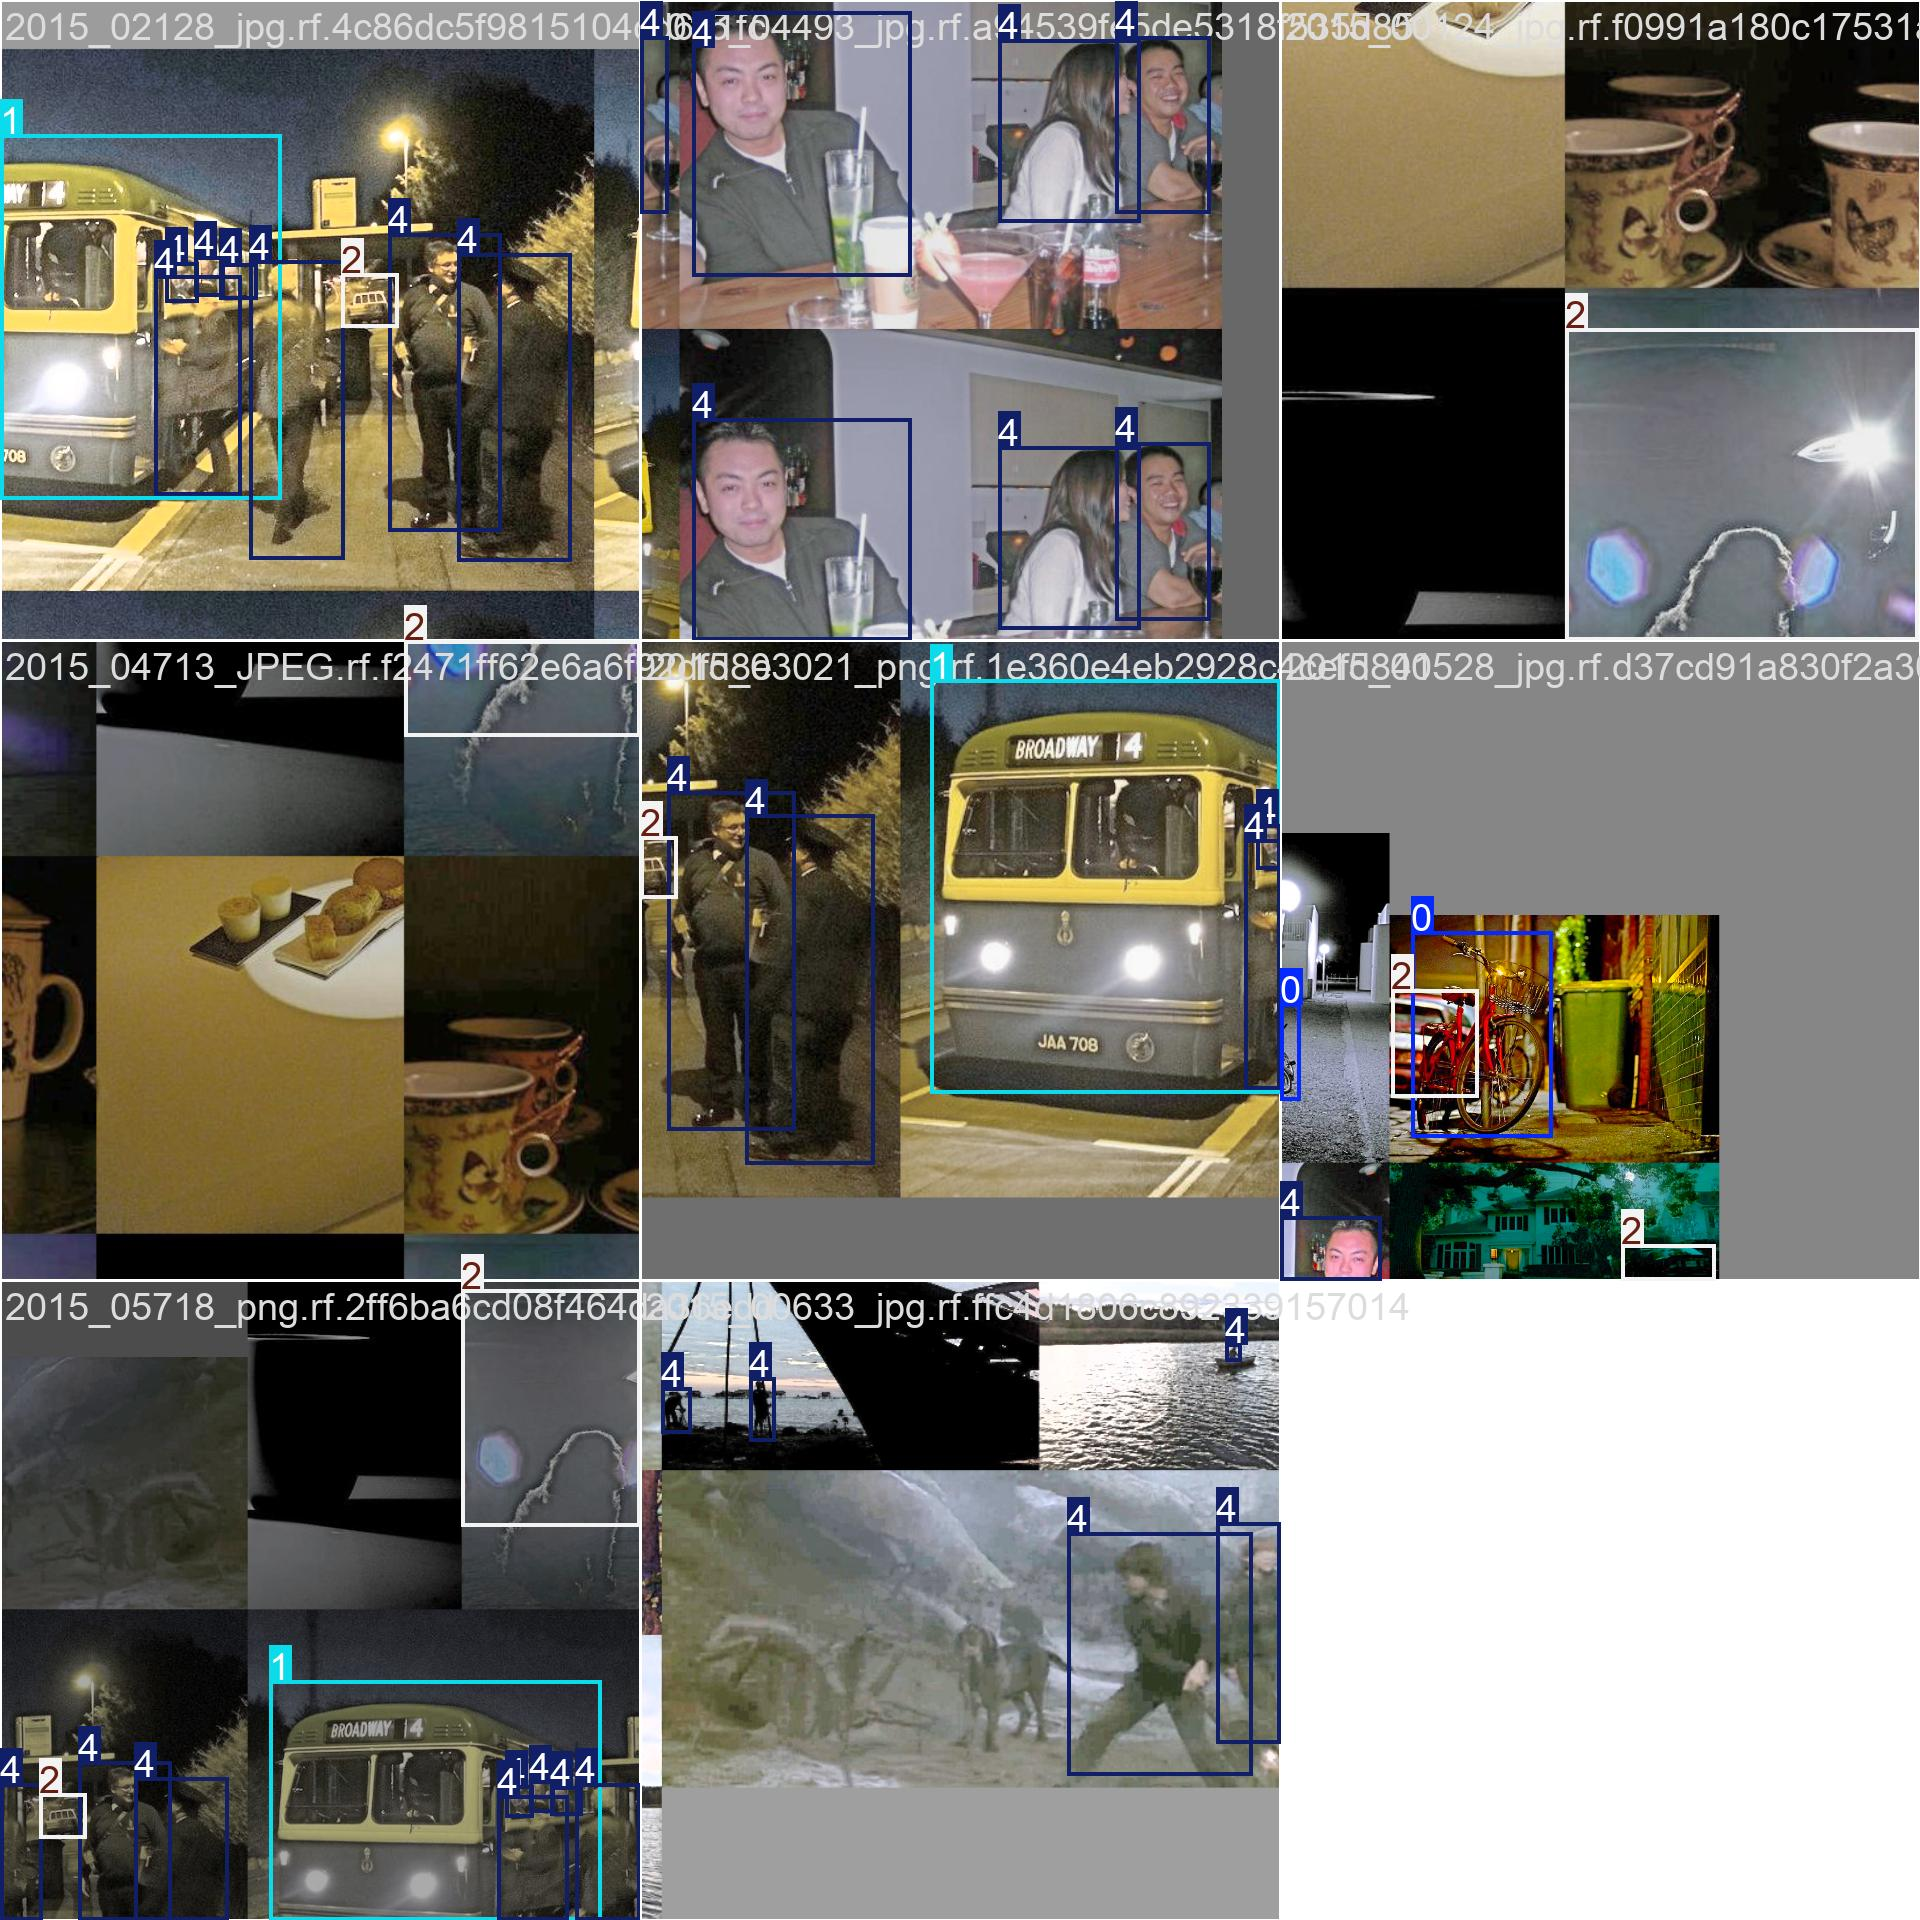
\includegraphics[width=\linewidth]{results/detection/night_traffic-2/train_batch2.jpg}\end{minipage}
\caption{Saved training-batch previews for Night Traffic.}
\end{figure}
\begin{figure}[t]\centering
\begin{minipage}{0.32\textwidth}\centering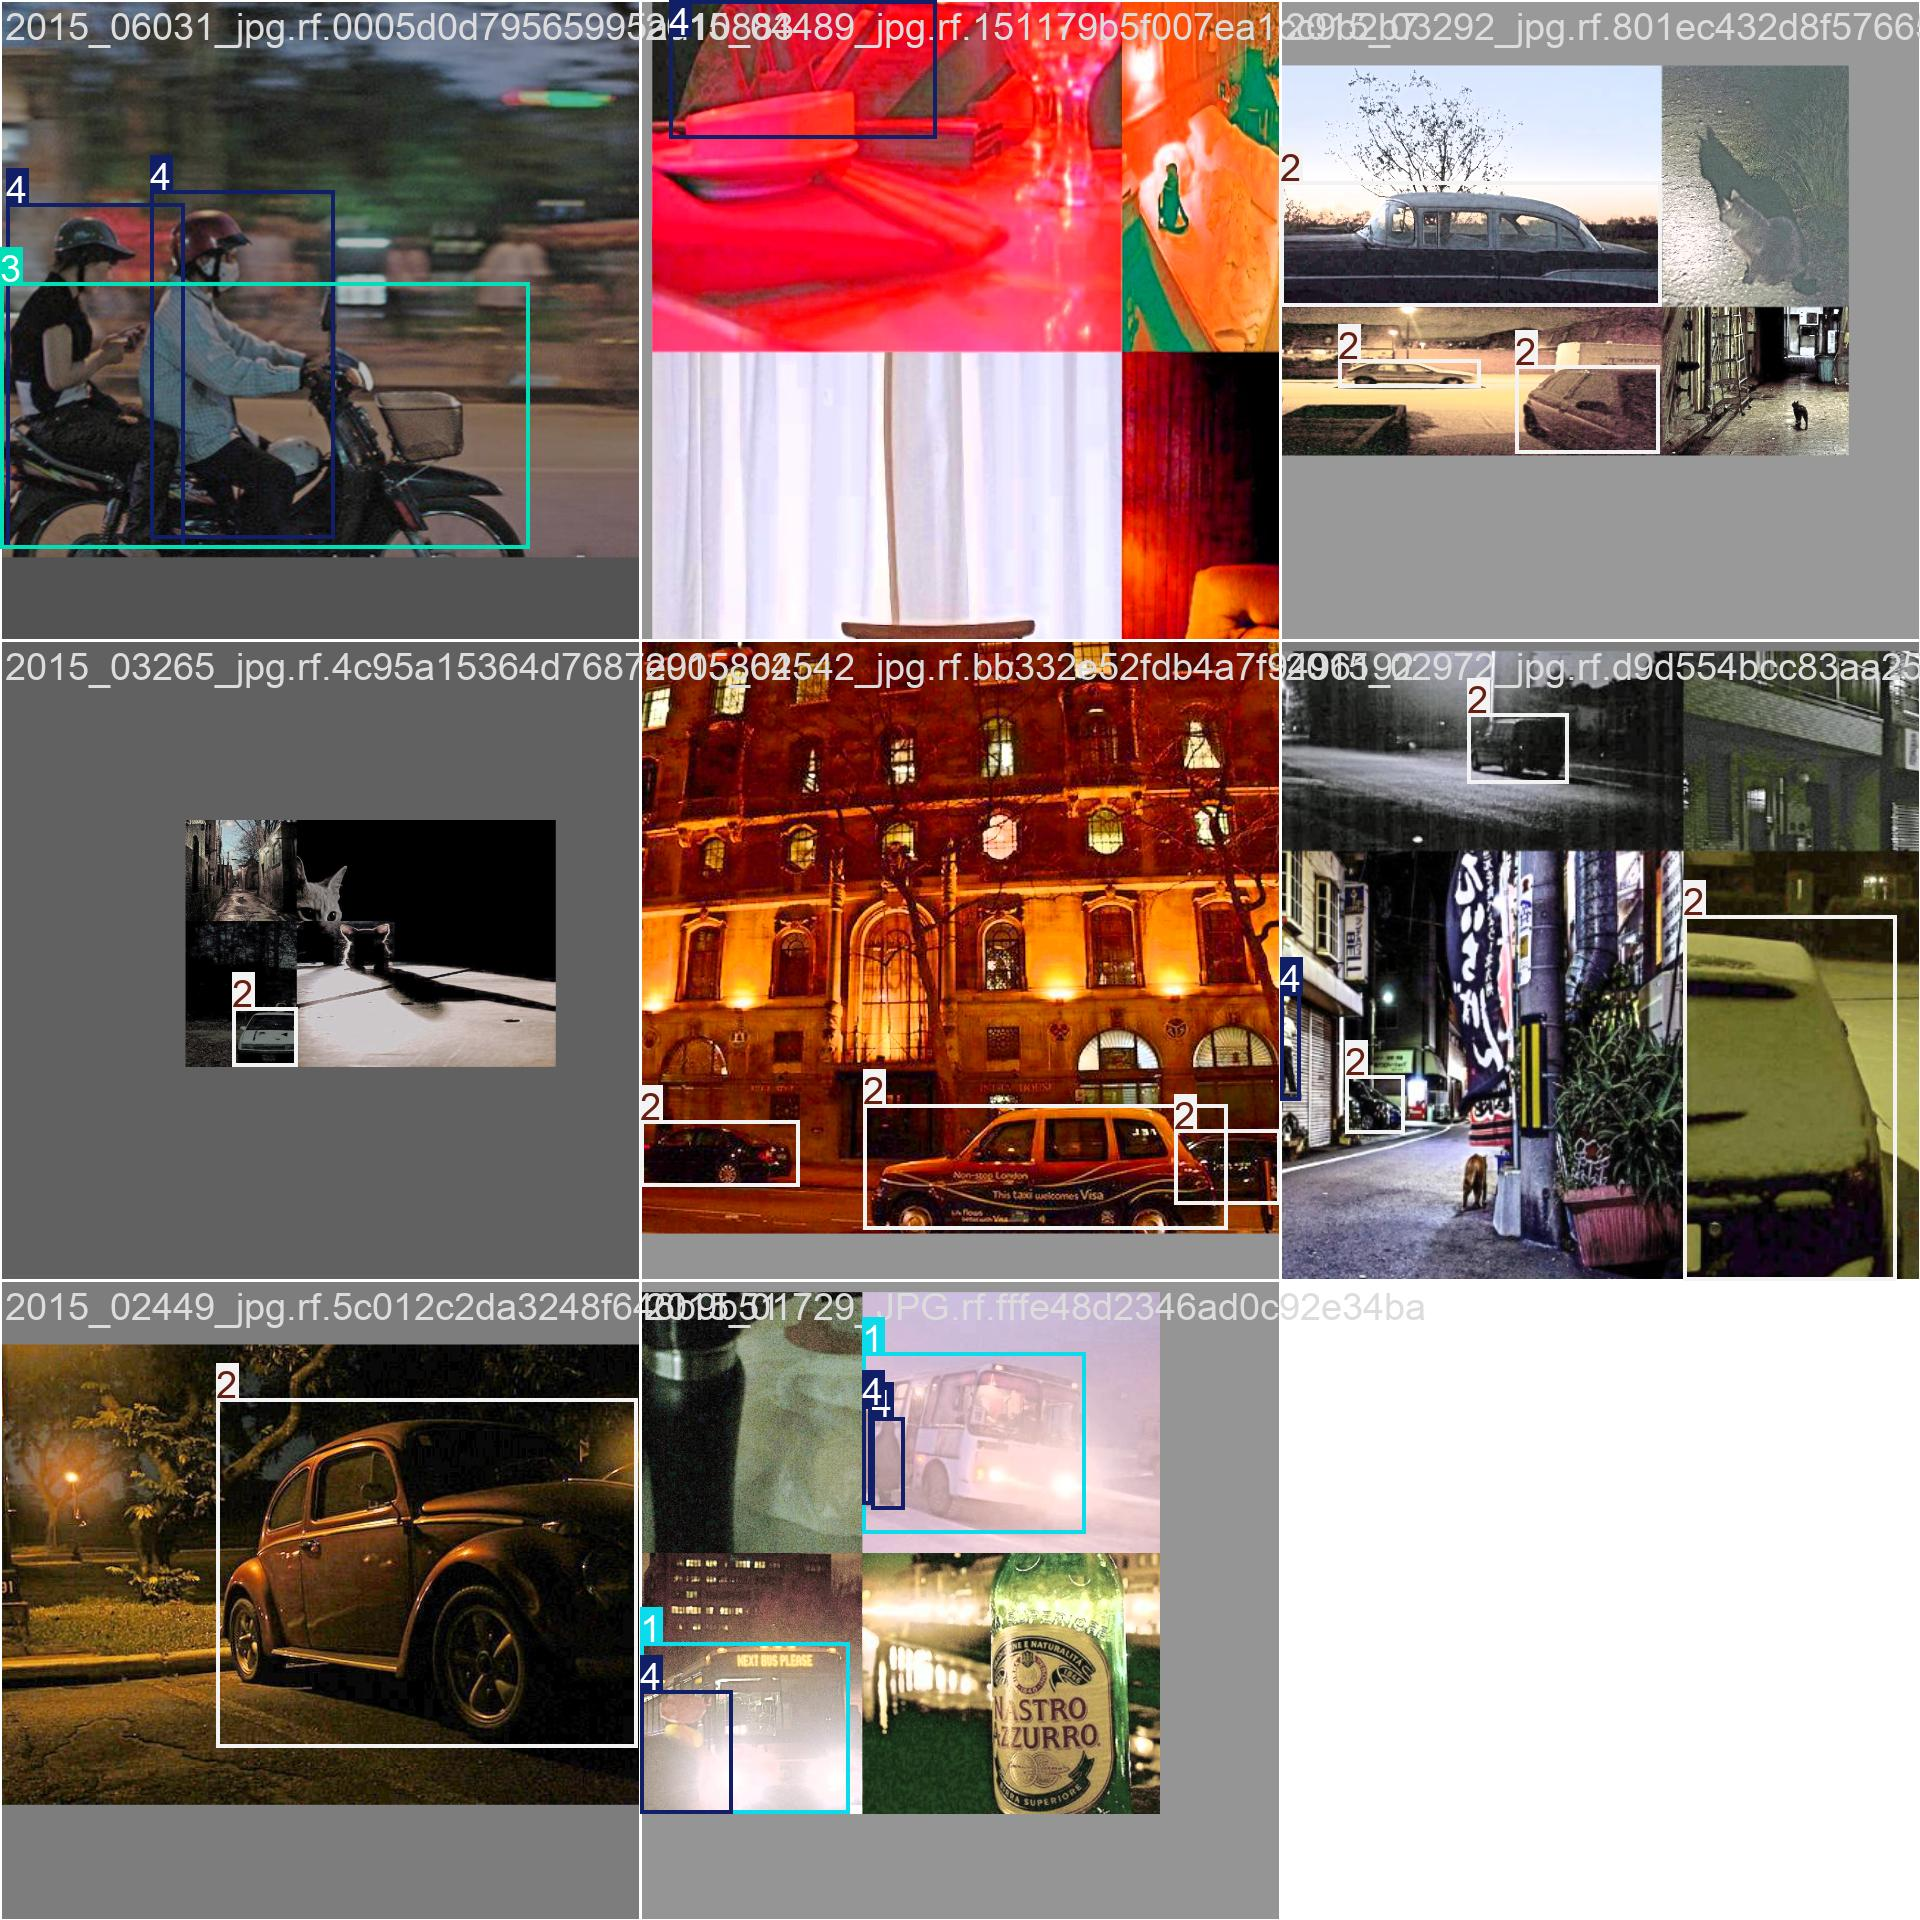
\includegraphics[width=\linewidth]{results/detection/night_traffic-2/train_batch79200.jpg}\end{minipage}
\begin{minipage}{0.32\textwidth}\centering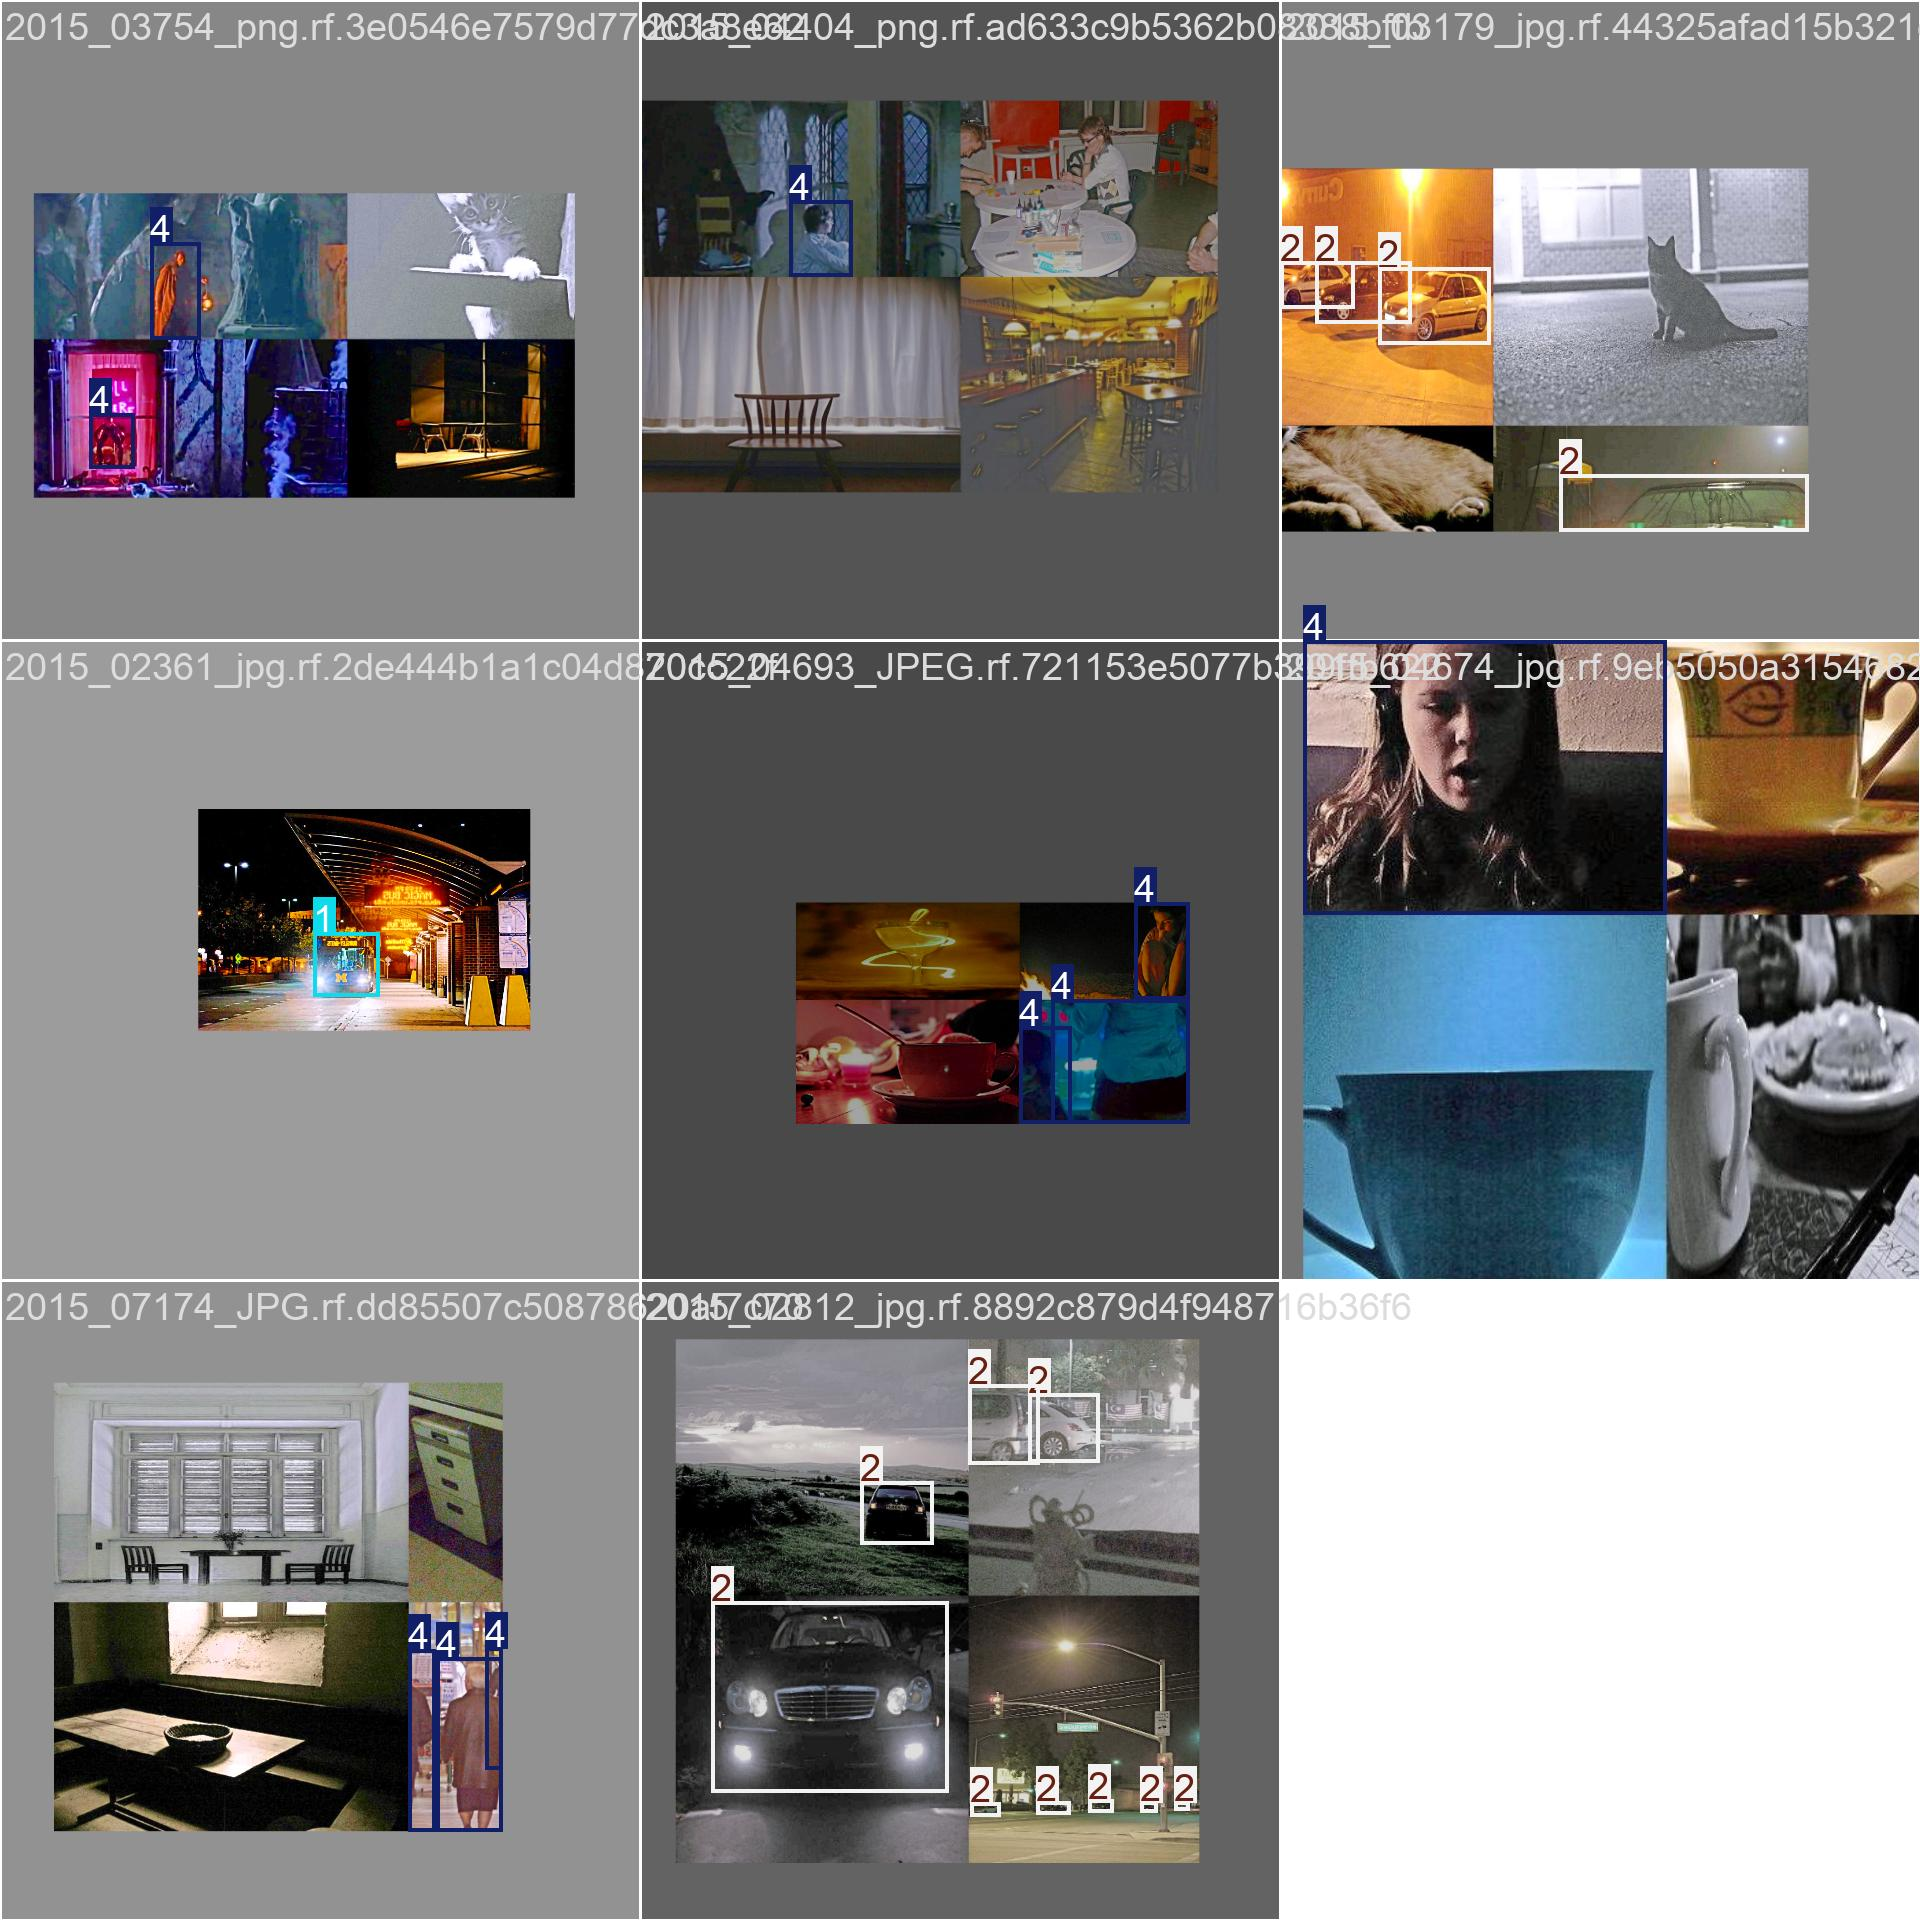
\includegraphics[width=\linewidth]{results/detection/night_traffic-2/train_batch79201.jpg}\end{minipage}
\begin{minipage}{0.32\textwidth}\centering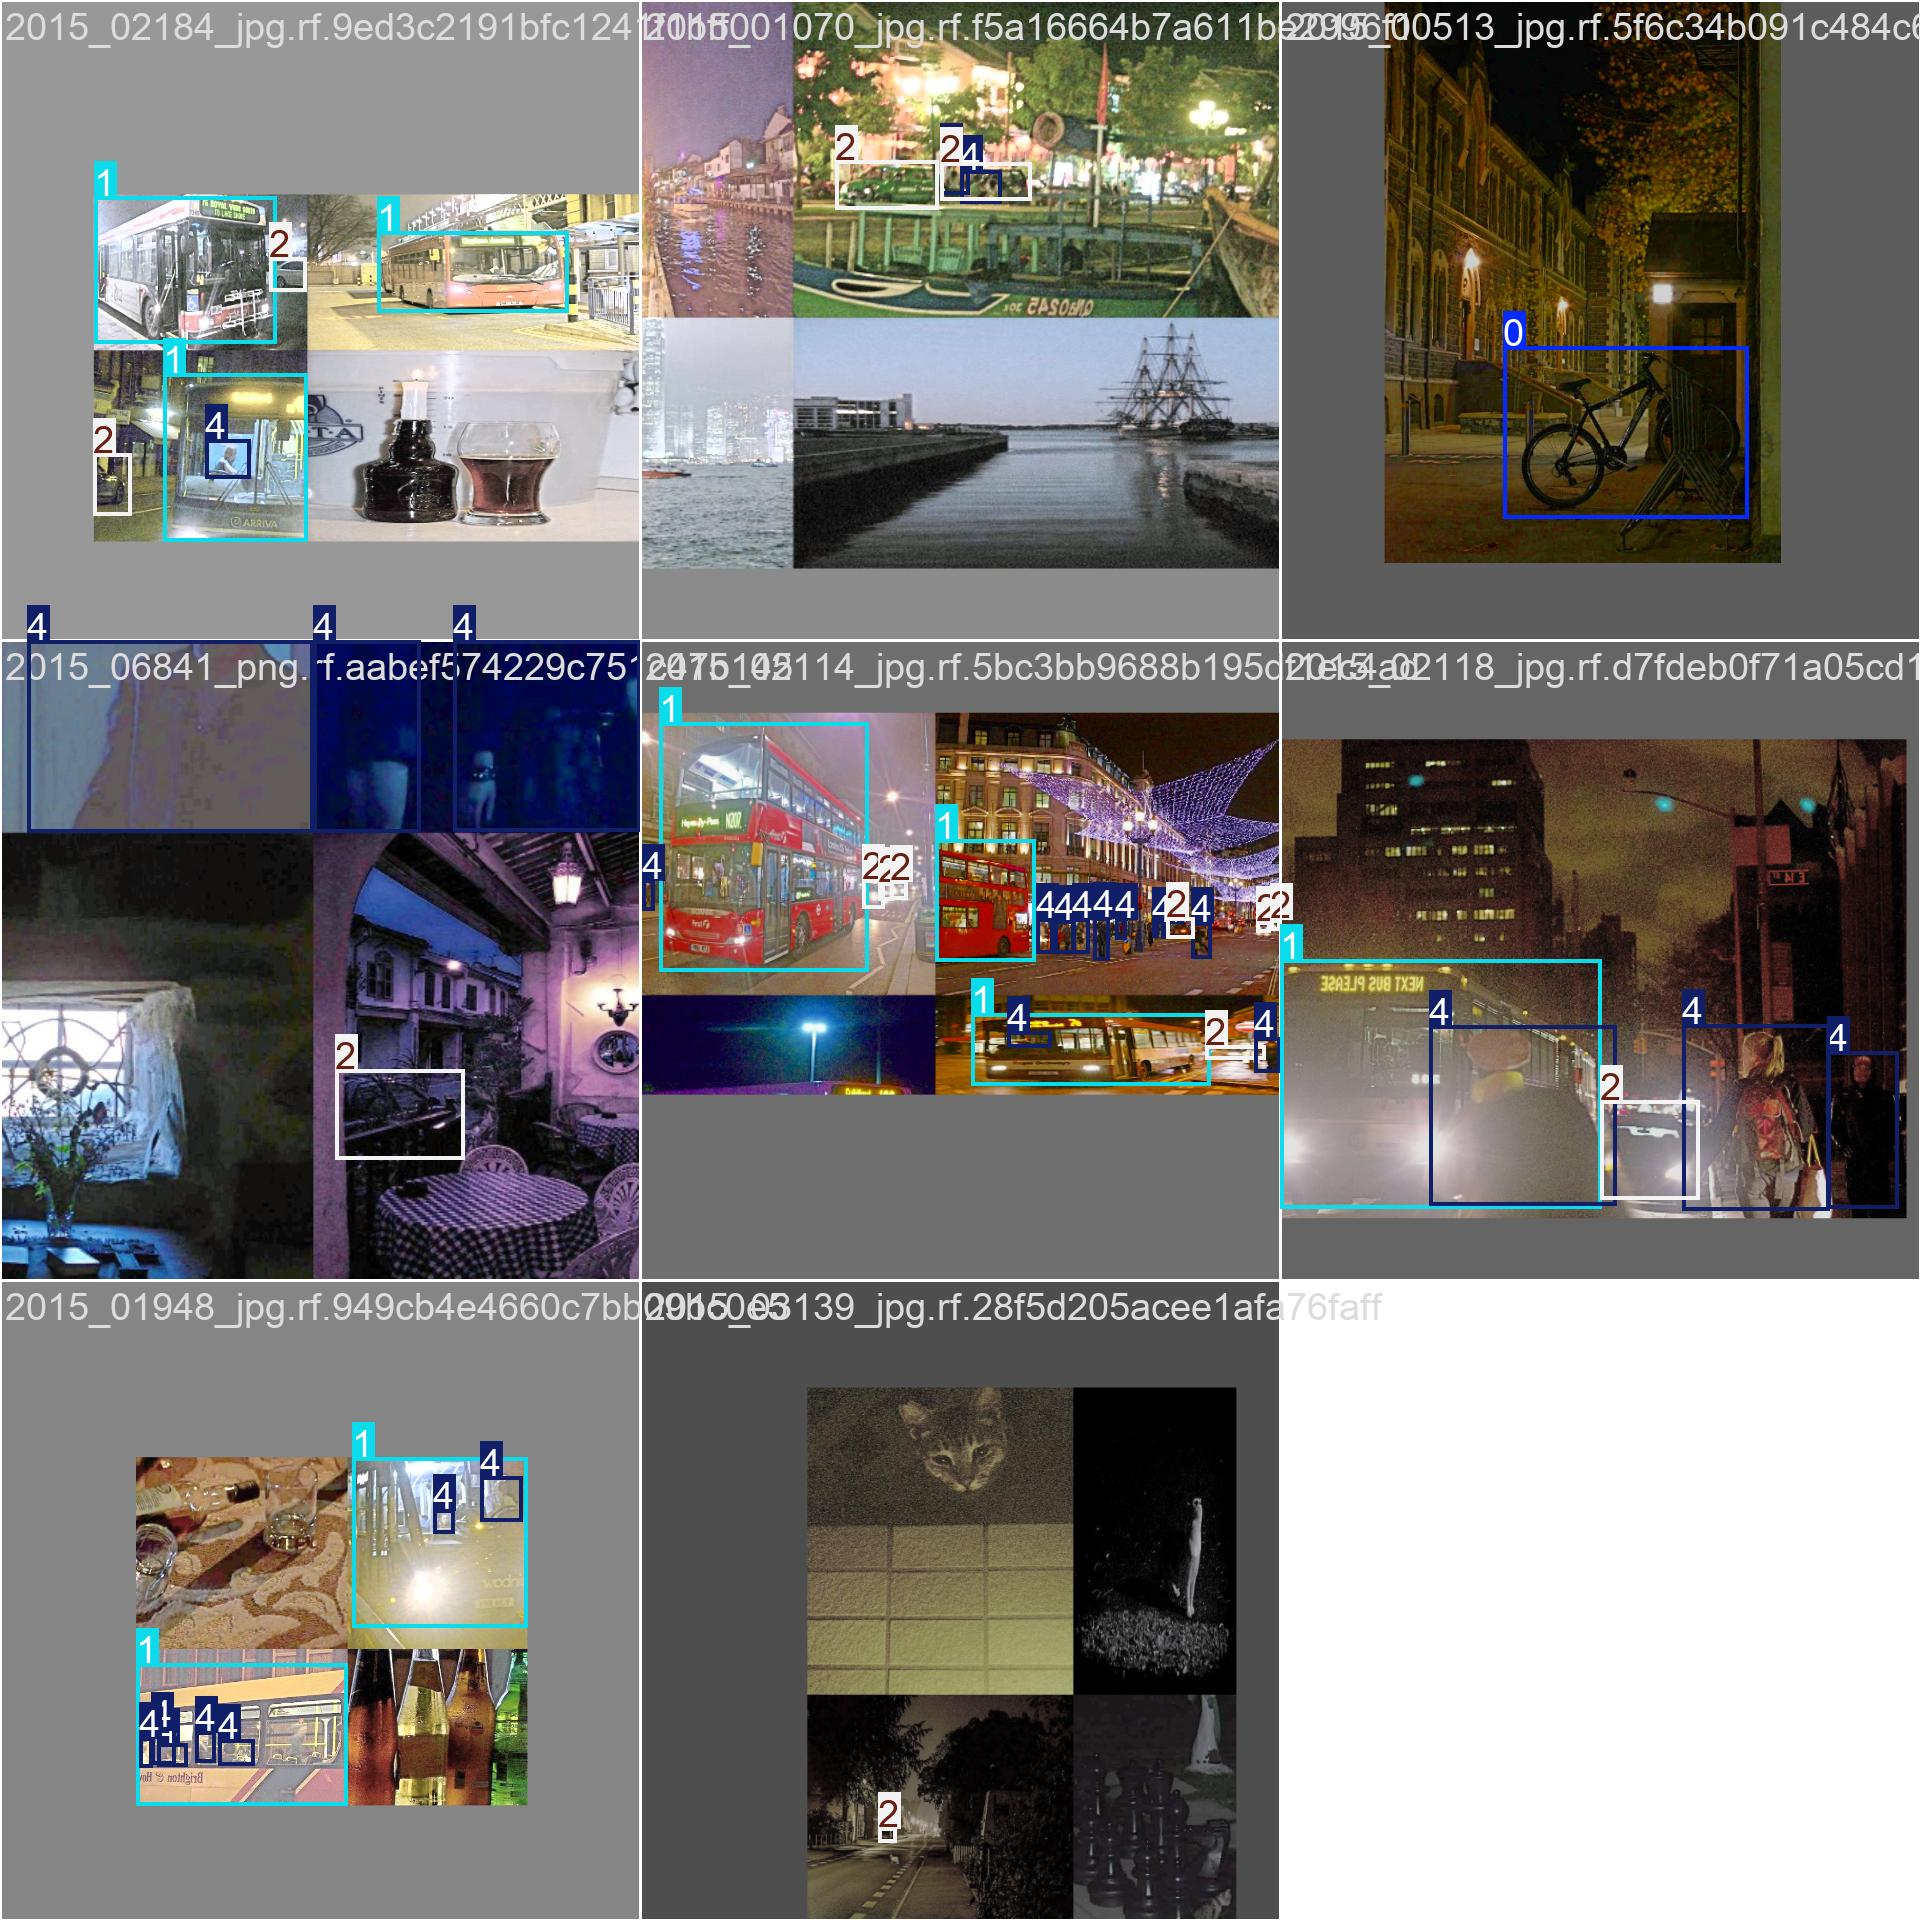
\includegraphics[width=\linewidth]{results/detection/night_traffic-2/train_batch79202.jpg}\end{minipage}
\caption{Saved training-batch previews for Night Traffic.}
\end{figure}
\begin{figure}[t]\centering
\begin{minipage}{0.32\textwidth}\centering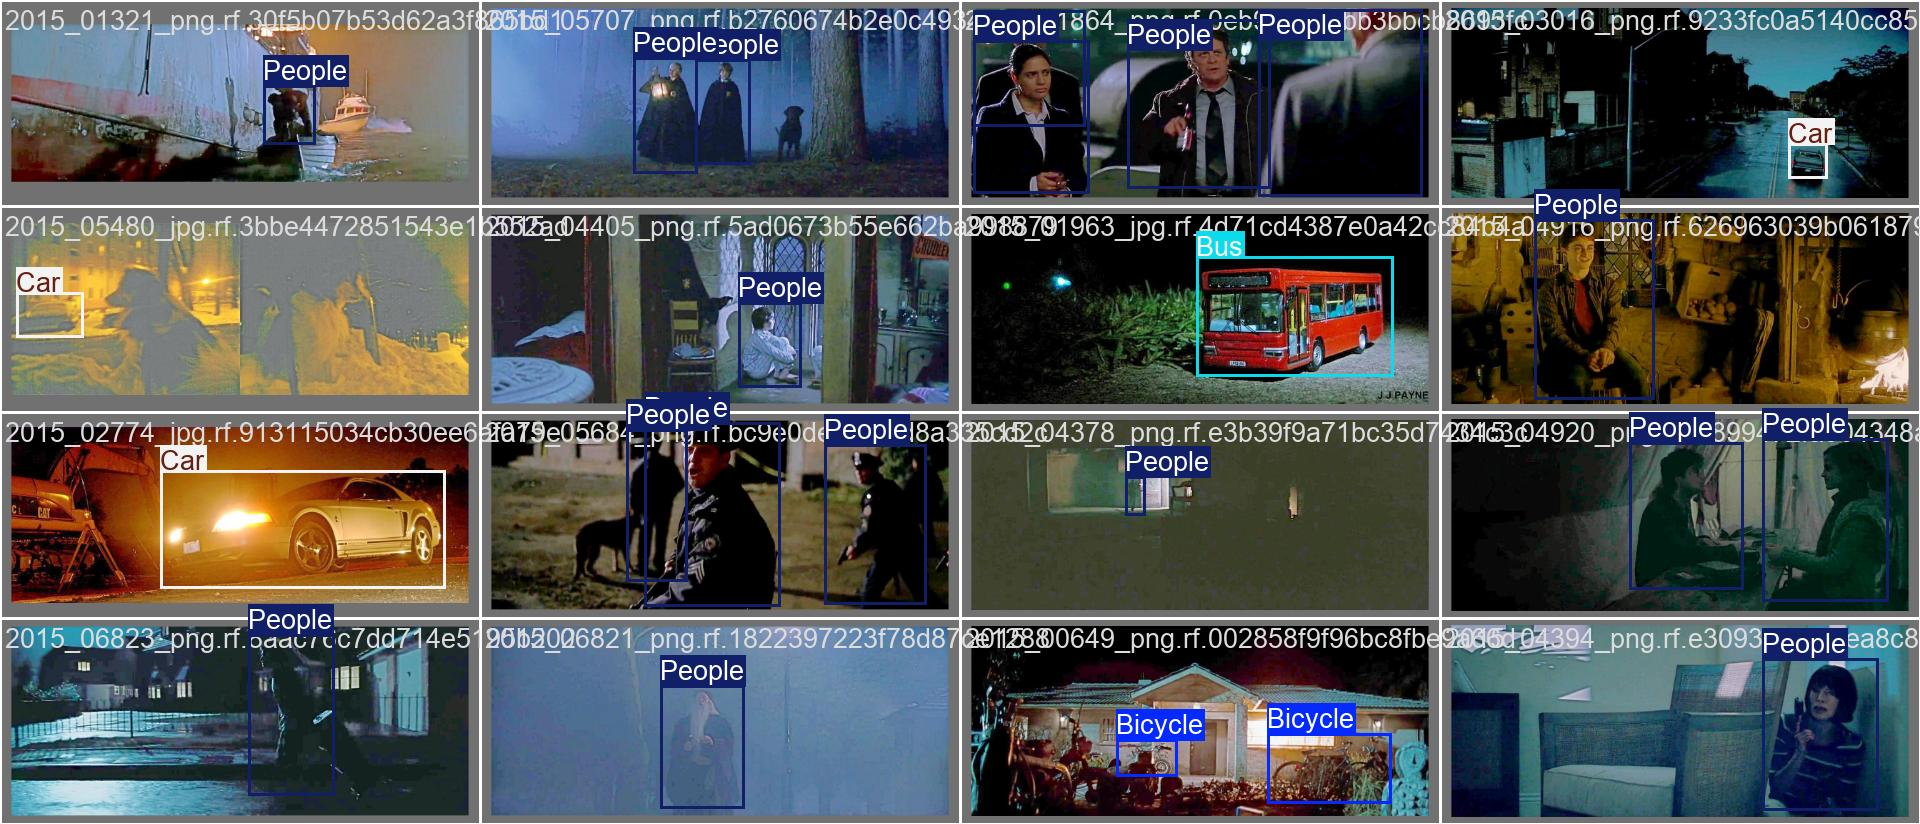
\includegraphics[width=\linewidth]{results/detection/night_traffic-2/val_batch0_labels.jpg}\end{minipage}
\begin{minipage}{0.32\textwidth}\centering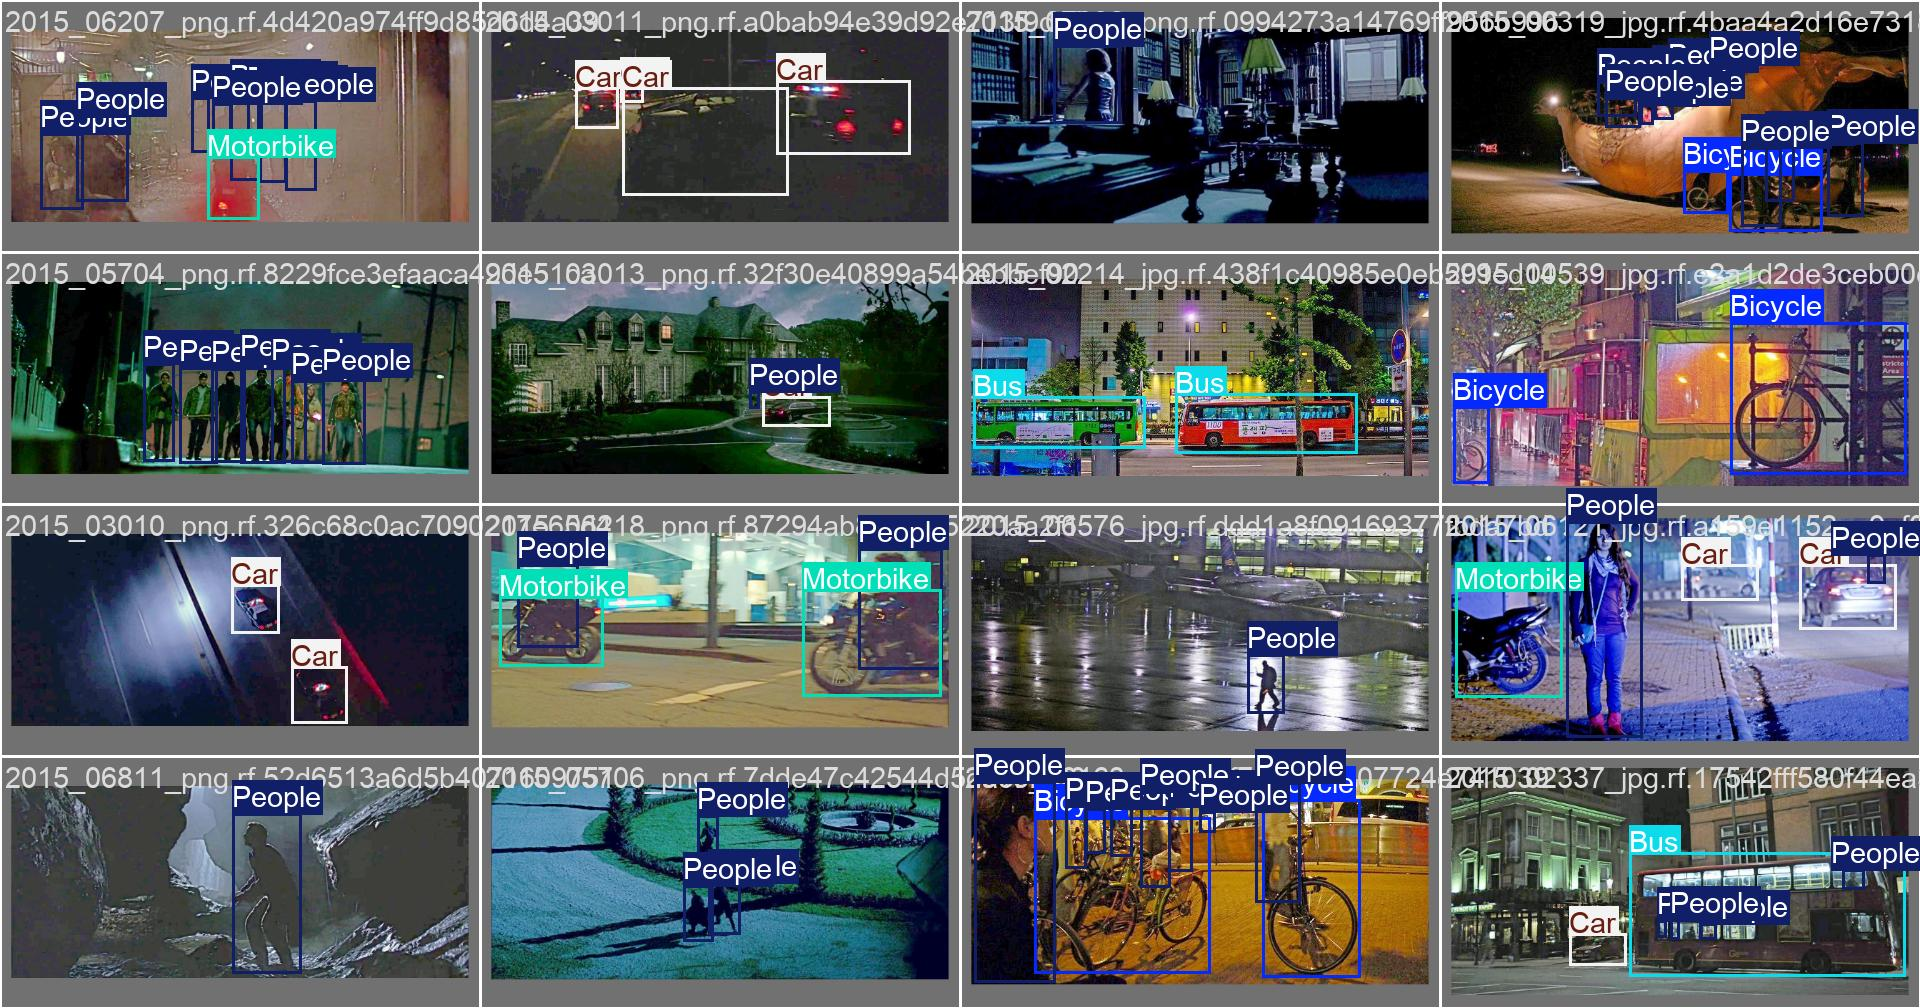
\includegraphics[width=\linewidth]{results/detection/night_traffic-2/val_batch1_labels.jpg}\end{minipage}
\begin{minipage}{0.32\textwidth}\centering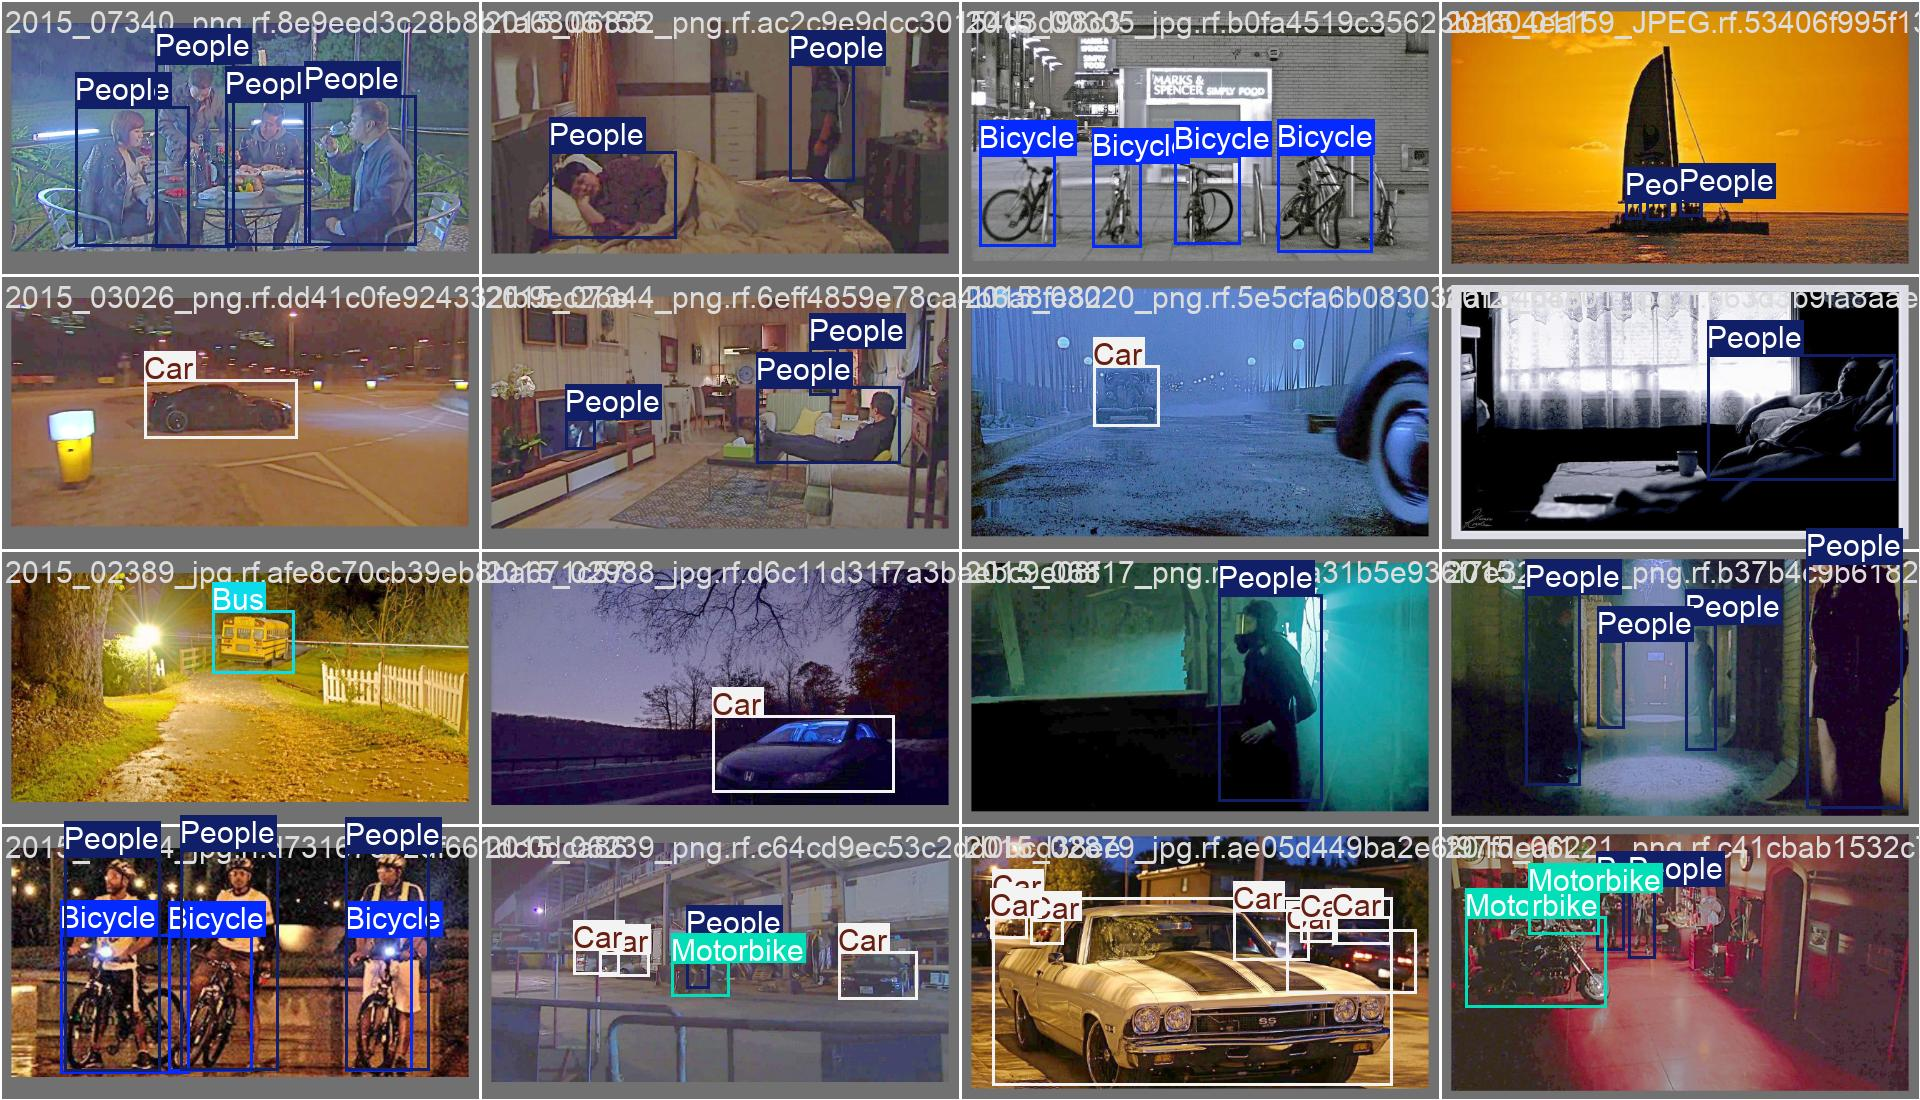
\includegraphics[width=\linewidth]{results/detection/night_traffic-2/val_batch2_labels.jpg}\end{minipage}
\par\vspace{4pt}
\begin{minipage}{0.32\textwidth}\centering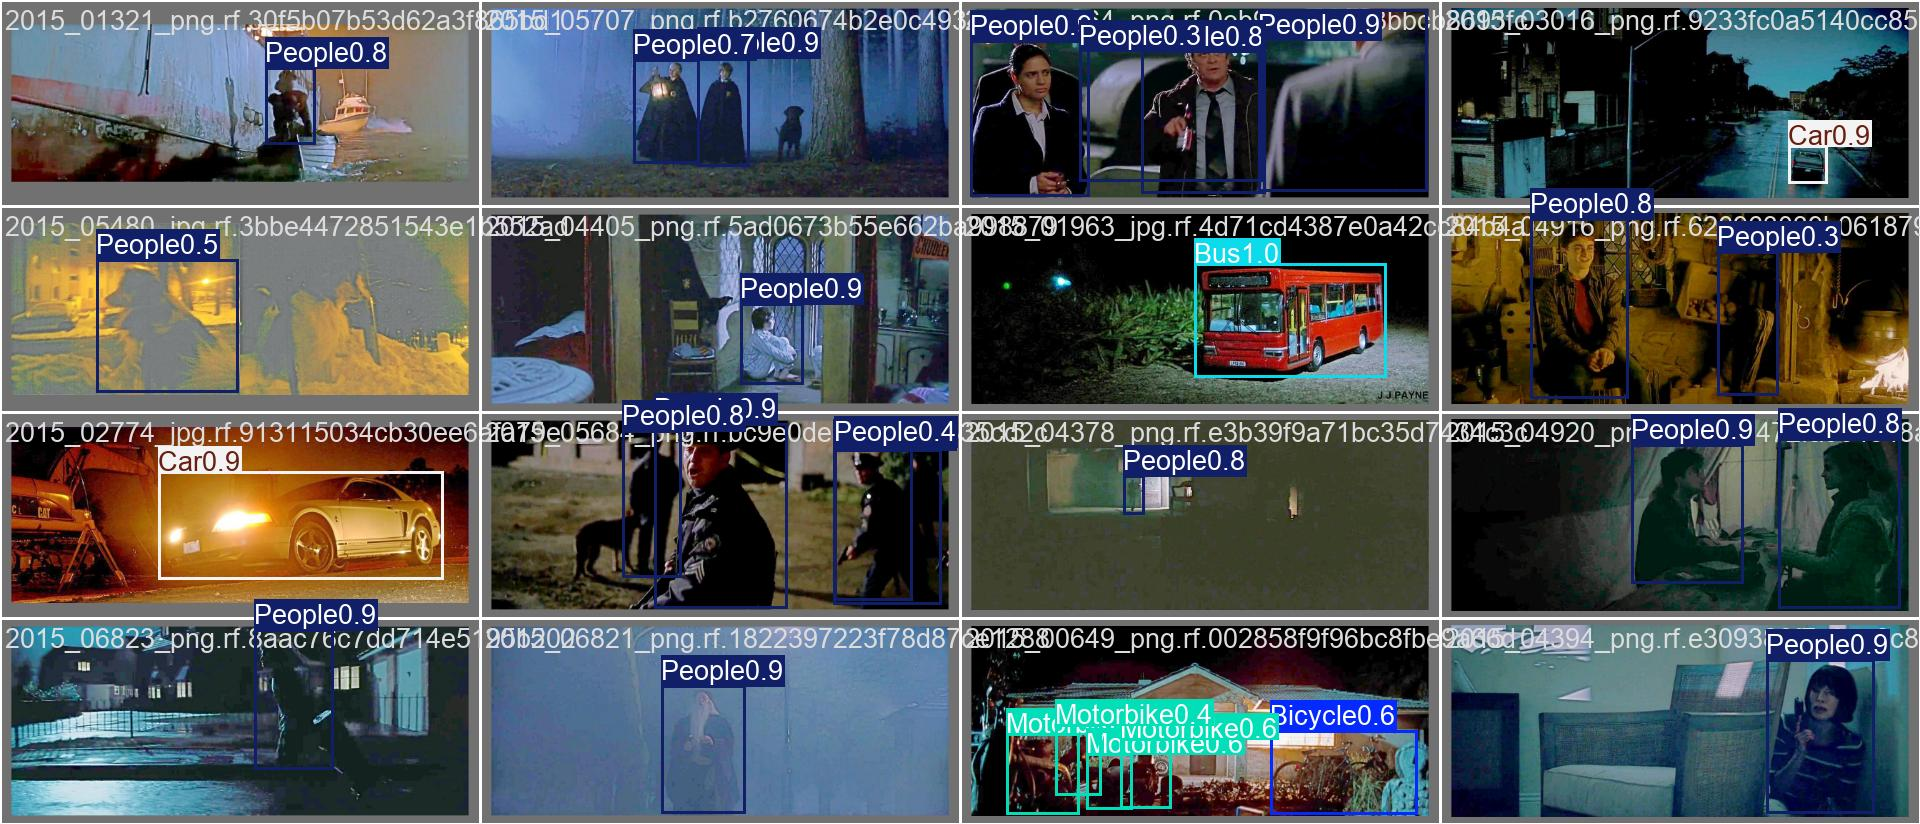
\includegraphics[width=\linewidth]{results/detection/night_traffic-2/val_batch0_pred.jpg}\end{minipage}
\begin{minipage}{0.32\textwidth}\centering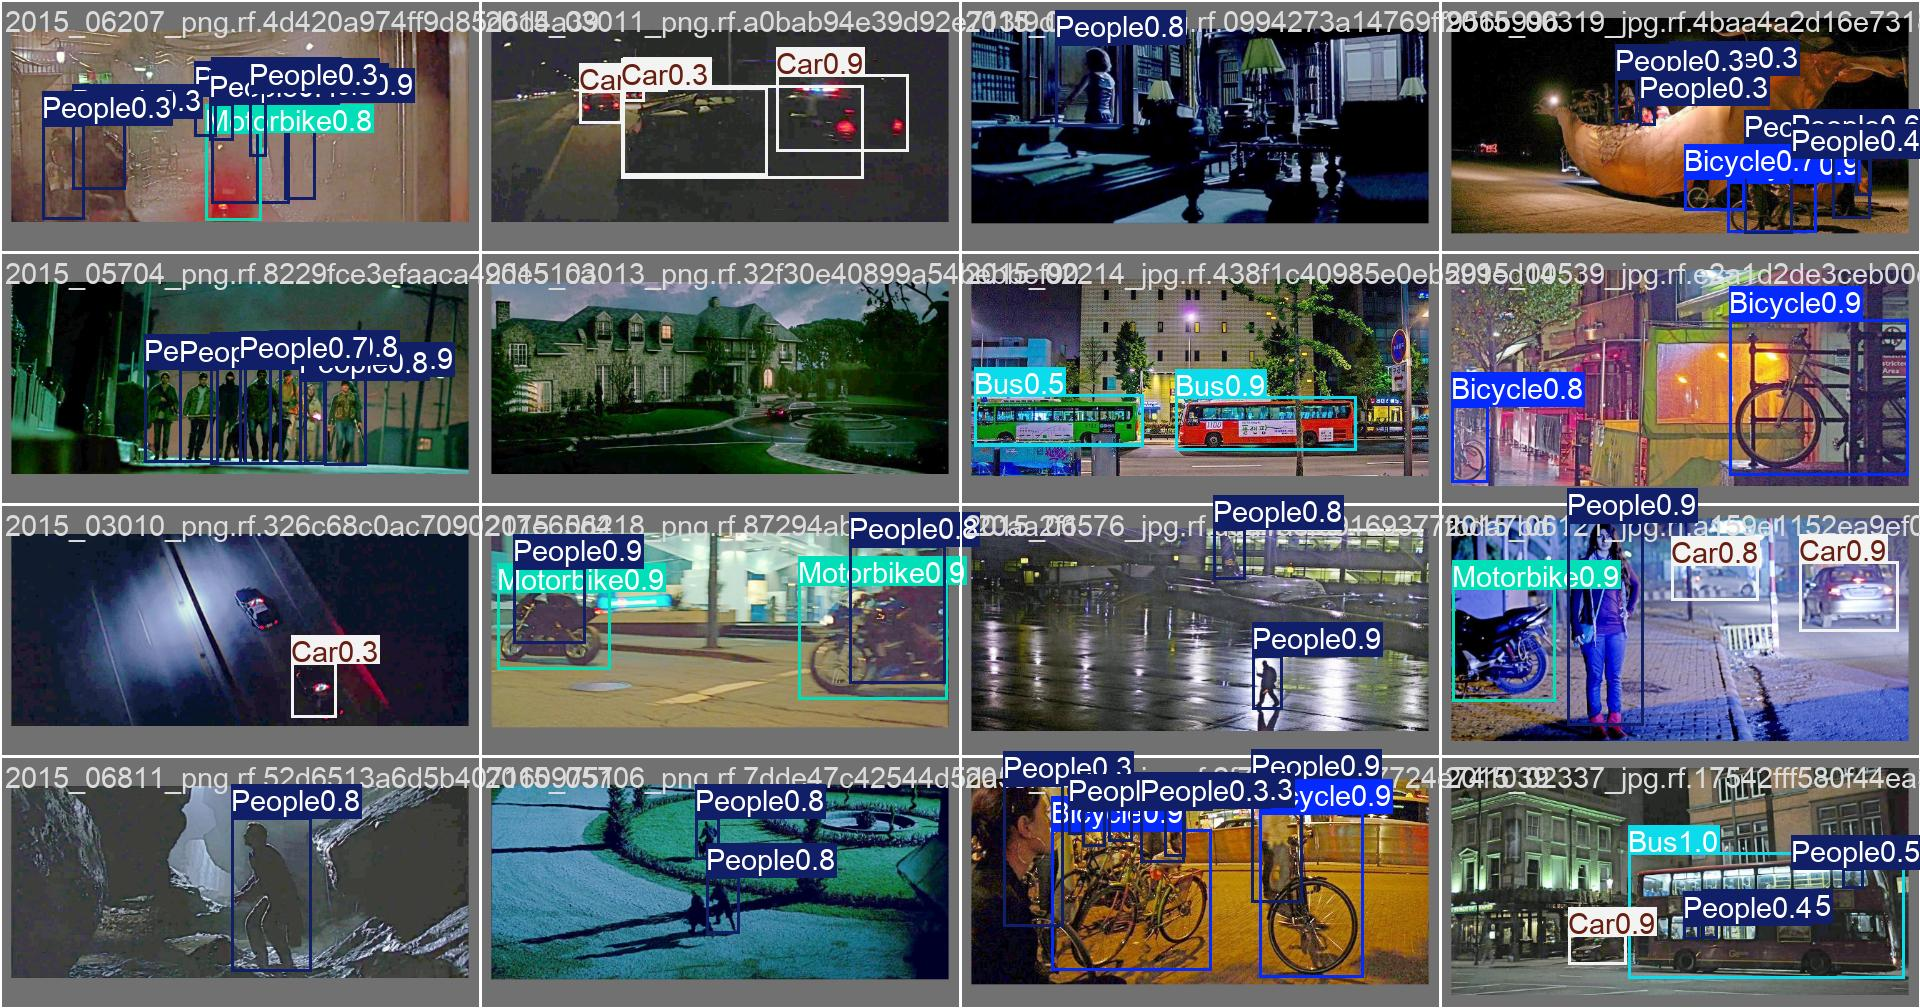
\includegraphics[width=\linewidth]{results/detection/night_traffic-2/val_batch1_pred.jpg}\end{minipage}
\begin{minipage}{0.32\textwidth}\centering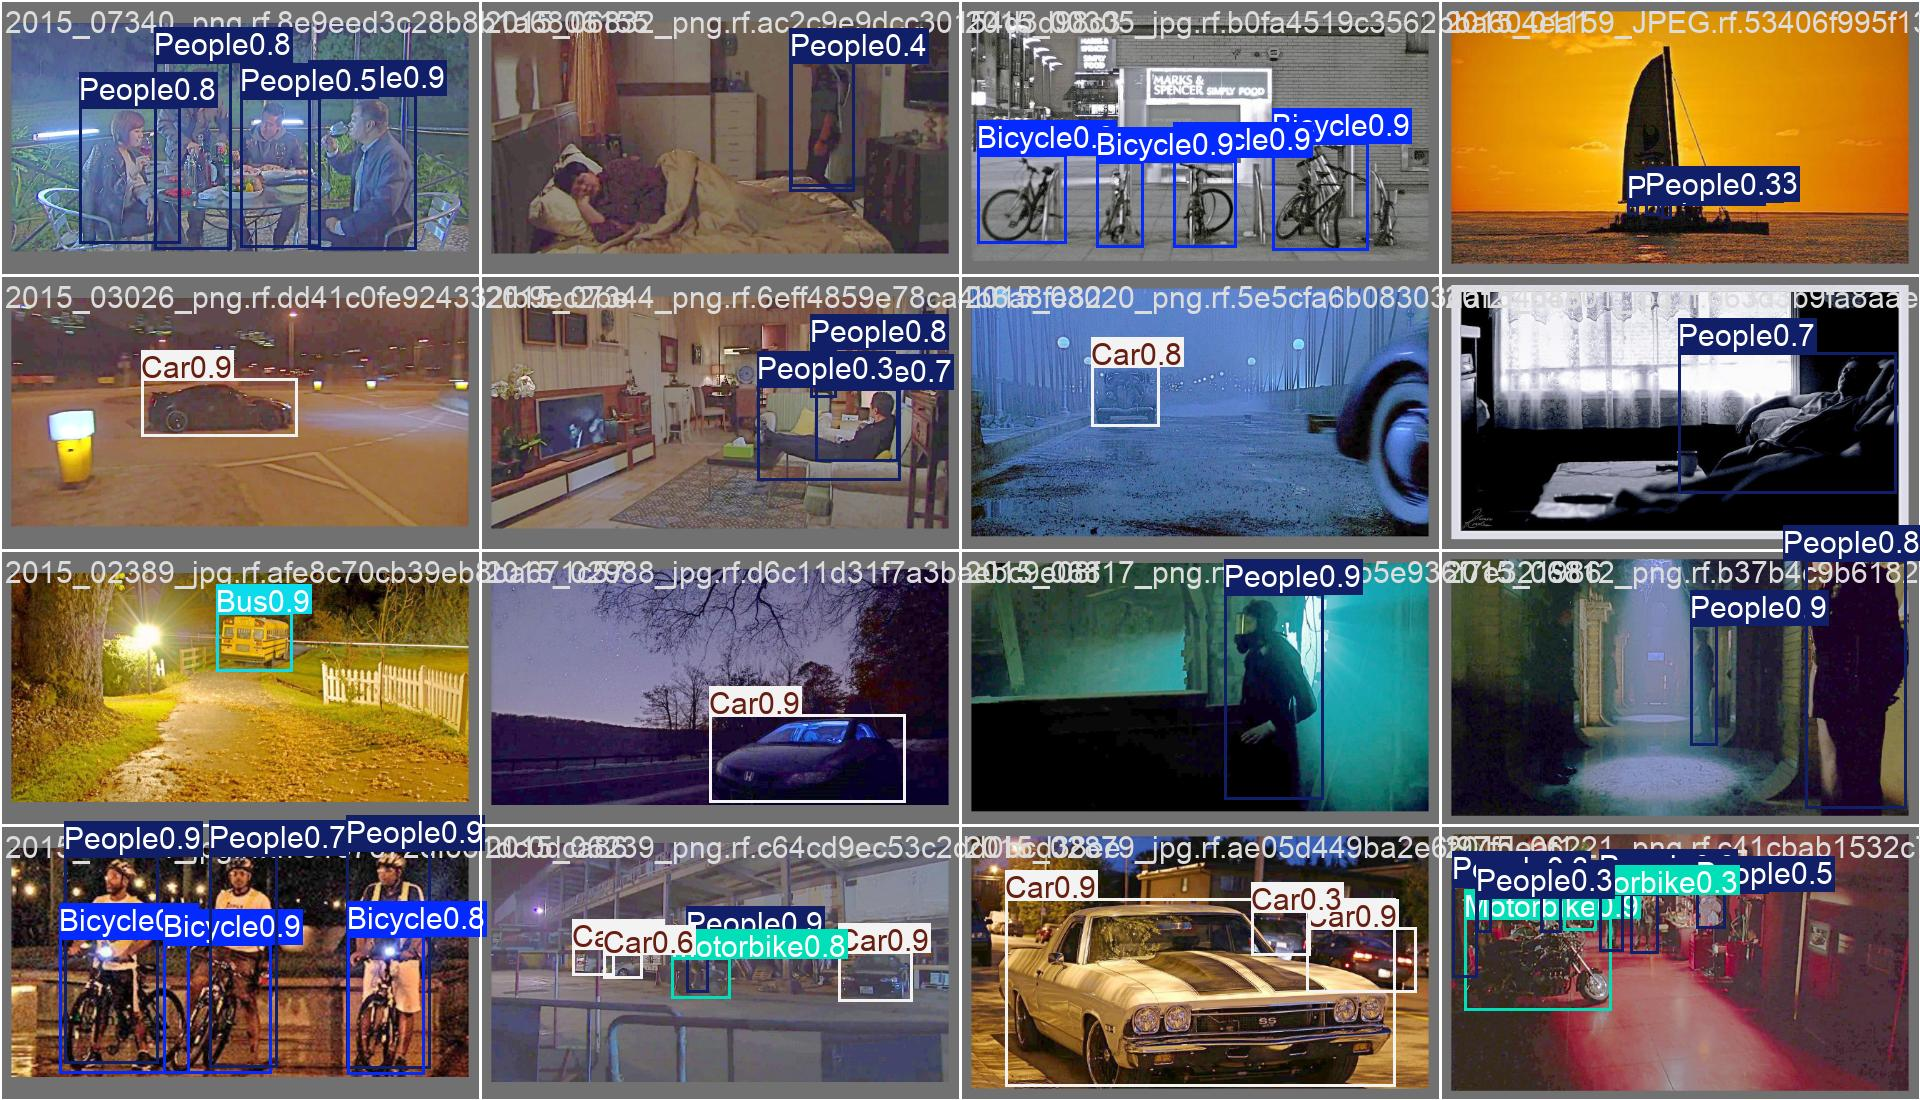
\includegraphics[width=\linewidth]{results/detection/night_traffic-2/val_batch2_pred.jpg}\end{minipage}
\caption{All saved validation batches for Night Traffic: ground-truth labels above and predictions below.}
\end{figure}
\section{Reproducibility and Artifact Checklist}
The saved folders contain model arguments, 100-epoch CSV logs, checkpoints, training curves, class curves, confusion matrices, label plots, training mosaics, and validation mosaics. Preserve the source commit, data licenses, dataset YAMLs, exact split manifest, checkpoint hashes, package versions, hardware details, and evaluation commands when archiving. The absolute dataset paths in saved arguments refer to an earlier location; the present project path requires confirmation before a fresh run can be described as reproduction. No new training or independent model evaluation was performed for this report.

\begin{thebibliography}{99}\small
\bibitem{who2023} World Health Organization, \emph{Global Status Report on Road Safety 2023}. Geneva, Switzerland: WHO, 2023.
\bibitem{repository} P. Aditya, G. S. Harsha, and M. Pallavi, ``AI Smart Accident Detection System,'' project source code, training runs, and generated result artifacts, supplied local repository, inspected Oct. 2026.
\bibitem{projectreport} P. Aditya, G. S. Harsha, and M. Pallavi, ``AI-Based Road Accident Detection, Severity Assessment and Emergency Alert System for Nearby Hospitals,'' capstone project presentation, Amrita Vishwa Vidyapeetham, supplied PDF, 2026.
\bibitem{fang2024} J. Fang, J. Qiao, J. Xue, and Z. Li, ``Vision-based traffic accident detection and anticipation: A survey,'' \emph{IEEE Transactions on Circuits and Systems for Video Technology}, vol. 34, no. 4, pp. 1983--1999, 2024, doi: 10.1109/TCSVT.2023.3307655.
\bibitem{shi2024two} L. Shi and F. Guo, ``Two-stream video-based deep learning model for crashes and near-crashes,'' \emph{Transportation Research Part C: Emerging Technologies}, vol. 166, art. 104794, 2024, doi: 10.1016/j.trc.2024.104794.
\bibitem{xu2022tad} Y. Xu, C. Huang, Y. Nan, and S. Lian, ``TAD: A large-scale benchmark for traffic accidents detection from video surveillance,'' arXiv:2209.12386, 2022.
\bibitem{zimmer2025} W. Zimmer et al., ``Towards Vision Zero: The TUM Traffic Accid3nD Dataset,'' in \emph{Proc. IEEE/CVF International Conference on Computer Vision Workshops}, 2025, pp. 852--862.
\bibitem{yu2024fine} H. Yu, X. Zhang, Y. Wang, Q. Huang, and B. Yin, ``Fine-grained accident detection: Database and algorithm,'' \emph{IEEE Transactions on Image Processing}, vol. 33, pp. 1059--1069, 2024, doi: 10.1109/TIP.2024.3355812.
\bibitem{picek2026} L. Picek, M. \v{C}erm\'ak, M. Hanzl, and V. \v{C}erm\'ak, ``ACCIDENT: A benchmark dataset for vehicle accident detection from traffic surveillance videos,'' in \emph{Proc. IEEE/CVF Conference on Computer Vision and Pattern Recognition Workshops}, 2026, pp. 685--694.
\bibitem{redmon2016} J. Redmon, S. Divvala, R. Girshick, and A. Farhadi, ``You only look once: Unified, real-time object detection,'' in \emph{Proc. IEEE Conference on Computer Vision and Pattern Recognition}, 2016, pp. 779--788.
\bibitem{redmon2018} J. Redmon and A. Farhadi, ``YOLOv3: An incremental improvement,'' arXiv:1804.02767, 2018.
\bibitem{jocher2026} G. Jocher et al., ``Ultralytics YOLO26: Unified real-time end-to-end vision models,'' arXiv:2606.03748, 2026.
\bibitem{ultralyticsval} Ultralytics, ``Model validation with Ultralytics YOLO,'' documentation, accessed Oct. 2026. [Online]. Available: \url{https://docs.ultralytics.com/modes/val/}
\bibitem{ade2024} V. A. Adewopo and N. Elsayed, ``Smart city transportation: Deep learning ensemble approach for traffic accident detection,'' \emph{IEEE Access}, vol. 12, pp. 59134--59147, 2024, doi: 10.1109/ACCESS.2024.3387972.
\bibitem{lin2014} T.-Y. Lin et al., ``Microsoft COCO: Common objects in context,'' in \emph{Proc. European Conference on Computer Vision}, 2014, pp. 740--755.
\bibitem{everingham2010} M. Everingham, L. Van Gool, C. K. I. Williams, J. Winn, and A. Zisserman, ``The Pascal Visual Object Classes (VOC) challenge,'' \emph{International Journal of Computer Vision}, vol. 88, pp. 303--338, 2010.
\end{thebibliography}

\end{document}
